%\RequirePackage{snapshot}
% !TeX encoding = UTF-8
% !TeX spellcheck = en_GB
\documentclass[12pt,
%    draft,     %taking out draft switches marginal notes off and pictures on
    ]{book} 
\usepackage{incremental_SS_Translation} 
\addbibresource{incremental_SS_Translation.bib}

% private macros for switching between chapters    
\newif \ifkalpa 
\newif\ifsarira 
\newif \ifjvara   
\newif\ifsutra
\newif\ifnidana
%
%\nidanatrue
%\kalpatrue
%\sariratrue
%\sutratrue


\title{Draft Translation of the Nepalese Version of the \emph{Suśrutasaṃhitā}}

\author{Dominik Wujastyk 
    \and Jason Birch
    \and Andrey Klebanov
    \and Lisa A. Brooks 
    \and Paras Mehta 
    \and Madhusudan Rimal
    \and Deepro Chakraborty
    \and Harshal Bhatt
    \and Jane Allred
    \and et alii}
\date{\texttt{Draft of \today}\\ \copyright\ The Authors}

\newcommand{\ignoreargument}[1]{\empty }



\ifkalpa 
    \includeonly{%chapters/translation 5-introduction,
    chapters/translation 5-introduction,
%        chapters/translation 5-08,    
} \fi
\ifsutra
\includeonly{%chapters/translation 5-introduction,
    chapters/translation 1-13,    
    %chapters/bibliography and indexes
} \fi
\ifsarira \includeonly{chapters/translation 3-03,
   % chapters/bibliography and indexes
} \fi       
\ifjvara  \includeonly{chapters/translation 6-39} \fi        
\ifnidana \includeonly{chapters/translation 2-01,
%    chapters/bibliography and indexes,
    } \fi

%
% from 
%https://tex.stackexchange.com/questions/361031/biblatex-how-to-automatically-sort-citation-by-year-sortcites-ynt-when-refere/361042#361042
\AtBeginRefsection{\GenRefcontextData{sorting=ynt}}
\AtEveryCite{\localrefcontext[sorting=ynt]}

\begin{document}
    
    \input{sanskrit-hyphenations}
        
    %\nocite{forb-1856}
    \pagecolor{cyan}
    \thispagestyle{empty}
          \maketitle

        \newpage
        \pagecolor{white}
        \tableofcontents
        
        % !TeX root = ../incremental_SS_Translation.tex

\chapter{Introduction}

What follows is a draft translation of selected chapters of the
\emph{Compendium of Suśruta} (\emph{Suśrutasaṃhitā}).  This differs
from former translations, being based on the text that survives in the
oldest known manuscripts of the work.\footnote{See \cite{wuja-2023}
    for an introduction to the Nepalese text and \cite{wuja-2021b} for
    background on the Suśruta Project, 2021--2024.}  These old manuscripts
    are located in Nepal, so we refer to this as “the Nepalese version” of
    the work, although future research may show that this old version was
    more widely known.\footnote{For more discussion of this issue, see 
    \cite[Introduction and ch.\,2]{wuja-2023}.}  
   
\section{The Nepalese Version}    

The Nepalese version has been reconstructed on the basis of three
manuscripts from Kathmandu,
    \begin{enumerate}
        \item \MS{Kathmandu KL 699} (siglum K),
        \item \MS{Kathmandu NAK 1-1079} (N), and
        \item \MS{Kathmandu NAK 5-333} (H).
    \end{enumerate}
The first of these MSS is the oldest, dated to
\CE~878.\footcite[15]{kleb-2021b}  It covers most of the \SS, but
lacks the \emph{Nidānasthāna} and the \emph{Śārīrasthāna} (see
Fig.\,\ref{fig:mss-1-visual-paradigm}).  The second is undated but is
datable on palaeographical grounds to the twelfth or thirteenth
centuries.\footcite[17--18]{kleb-2021b} It contains the
\emph{Sūtrasthāna} and \emph{Nidānasthāna} but breaks off shortly
afterwards.  The third manuscript, H, is the most complete, supporting
the text of the whole of the \SS. It is dated \CE~1513.\footnote{I
    follow the arguments of \citet[21--26]{kleb-2021b} on the
    interpretation of the colophon although, as he pointed out, some
    interpret the date as \CE\ 1573.} %
    The text of manuscript H follows K very closely but is probably
    not a direct apograph.\footcite{chak-2022} I conjecture that it
    was either copied from an intermediary that followed K very
    closely or from a ancestor of K.\footnote{“\ldots as neither my
        own research \ldots\ nor the study undertaken in Harimoto \ldots\
        could determine any linear connection between any of the Nepalese
        manuscripts of the SS, one may assume that [there exists] an older
        common ancestor of both of the manuscripts K and H.”
        \citep[21]{kleb-2021a}.}
        
        \begin{figure}[t]
            \centering
            \includegraphics[width=\textwidth]{"media/MSS 1 visual paradigm.art"}
            \caption{Coverage of the text by MSS K, N and H.}
            \label{fig:mss-1-visual-paradigm}
        \end{figure}
        
\section{The vulgate}

The version of the \SS\ that we refer to as “the vulgate” is the
version of the text that circulates in print today in multiple
editions.  The most careful and authoritative edition is that of
\citet{vulgate}.\footnote{This and the following issues have been
    discussed by \citet[2 and ch.\,3]{wuja-2023}.}  It is telling that
    this edition includes the commentary of Ḍalhaṇa (b.\ ca.\ 1175) and,
    for the \emph{Nidānasthāna}, also that of Gayadāsa (fl.\ ca.\ 1000).
    These important authors commented on a text that is, broadly speaking,
    what we call “the vulgate.”  But they both mentioned quite often that
    the manuscripts they were consulting contained other versions of the
    text and in a high number of cases, these variations match the
    Nepalese version.\footnote{E.g., see the discussion in footnote
        \ref{ancient-variants} below.}  It is possible that Gayadāsa  and Ḍalhaṇa,
        through their commentarial work on the text, participated in shaping
        “the vulgate."

The scholar Rudolph Hoernle was also aware of this cleavage in the
transmission-history of the \SS.  But with the more limited materials
available to him at the turn of the twentieth century he drew the line
a little differently.  He referred to the text of the
\emph{Śārīrasthāna} of the \SS, transmitted in the printed editions of his day, as
“the Traditional Recension."
\begin{quote}
    The recension which is found in Jīvānanda's and all other
prints,\footnote{Hoernle listed four,
    \cites{bhat-1889,gupt-1835,govi-1901,vira-nd}.} and which, in the
    sequel, will be referred to as the Traditional Recension, has in
    its favour not only all available manuscripts, but also all
    ancient commentaries on the Compendium of Suśruta, \ldots.  Or,
    shortly, the Traditional Recension is supported by the whole body
    of existing witnesses.\footcite[68]{hoer-1907}
\end{quote}
However, Hoernle was unfortunately not aware of the Nepalese
manuscripts of the \SS, which at the time he was writing were in
Nepalese libraries that had not yet been explored by scholars of the
time.  The contrast that Hoernle was drawing was between the
Traditional Recension and the \emph{Śārīrasthāna} of the \CS\ as
printed by the influential Bengali scholar, Kavirāja Gaṅgādhara Ray
(1798--1885).\footnote{\cite{gang-1868}.  Hoernle's evaluation of this
    edition was not entirely kind: “I have not been able to discover for
    it any authority whatsoever. \ldots\ it is probably that the recension
    of Gangādhar is a reconstruction of his own to meet those of the
    difficulties which he had noticed” \citep[70]{hoer-1907}.  For a full
    account of the genesis of this edition, see \cite{pecc-2022}.}

    
\section{The Translation}    
The translation follows the methods of rigorous philological care and
modern principles of translation theory.\footnote{See
    \cite[intro.]{wuja-2003} and \cite[81--83]{wuja-2021} for an
    overview.}  Major differences in sense from the vulgate text are
    marked  \diff{in this manner}, but the differences are so pervasive
    and fine-grained that most have not been explicitly marked.

The text-historical state of the \SS\ bears many resemblances to other early 
textual transmissions in South Asia.  The situation was articulated particularly 
clearly for the case of Pāli by \citet{hinu-1978}, in the opening of his chapter, 
\begin{quote}
    \ldots we cannot go back beyond the council of Aluvihāra (Ālokavihāra) under 
    Vaṭṭagāmaṇī Abhaya (29--17 B.C.) where the Pāli canon ws written down for 
    the first time in Ceylon.  This is the very starting point of our tradition 
    handed down to us by the monks of the Mahāvihāra.  About recensions of 
    the Pāli canon different from the Mahāvihāra tradition and deviating from its 
    wording\ldots\ we scarcely have any knowledge at all.
\end{quote}
Similarly, the manuscript evidence for the \SS\ that is available
today allows us to reconstruct a version of the work after it was
consolidated into a text of five parts with a sixth or “later”
(\emph{uttara}) and somewhat different part already appended to the
first five.  The prehistory of the work before this form is
tantalizingly unknown to us.  That the work was assembled from diverse
sources and that many hands were involved is without doubt. The oldest
surviving manuscript, \MS{Kathmandu KL 699}, gives us physical
evidence for the state of the text in the ninth century.  We little
insight into the formational processes affecting the text before that
time.  But what we can see plainly is that the text was edited
pervasively after that time, being influenced especially by the
commentators Jejjaṭa, Candraṭa, Gayadāsa and Cakrapāṇidatta and the
editor Candraṭa. However, a clear picture of how these later editorial
processes took place will only be possible as a result of further
research into a wider manuscript base.
            \thispagestyle{empty}
        
        \part{Part 1. Sūtrasthāna} 
                        
        % !TeX root = ../incremental_SS_Translation.tex

\chapter{Sūtrasthāna 1: The Origin of Medical Knowledge}

\section{Literature}

Meulenbeld offered an annotated overview of this chapter and a bibliography
of earlier scholarship to 2002.\fvolcite{IA}[203--204]{meul-hist} 

\section{Translation}

\begin{translation}
    
    \item[1] 
    
“Now I shall narrate the chapter on the origin of this
knowledge.\footnote{Ḍalhaṇa understood the word
    “\se{veda}{knowledge}" as specifically  “medical knowledge." He
    said that the word  “longevity" (\emph{āyur}) \ssaneng{āyur}{life,
    longevity} had been elided. %
    %    Notes Dec 8:
    %    Dominik: N's ādhyāyaṃ corruption of H's nāmādhyāyaṃ:
    % possible evidence that N was
    %created
    %after H
    %    Check: Ācārya 1931 footnote on vedotpattim
    %    Commentary Ḍalhaṇa (c. 1200 CE) notes āyur dropped from veda
    % in vedotpattim
    %
    %
    After this opening statement, later manuscripts and commentaries
    include the attribution,  “as the venerable Dhanvantari stated." 
    The absence of this statement in the early Nepalese manuscripts
    is highly significant because it removes the outer narrative
    frame of the \SS\
    \parencites[148]{wuja-2013}[\S\,3.1.2]{kleb-2021b}{rai-2019}{birc-2021}.  
    On the figure of Dhanvatari in medical literature, see \cite[IA 
    358--361]{meul-hist}.} %     <!-- Notes Dec 8:
    %    Dom: note the omission of Dhanvantari, which is in the
    % edition.
    %    On Dhanvantari, see Meulenbeld HIM, authorities associated
    % with Suśruta. He's
    % an authority on
    %surgery or toxicology-->
    
    \item[2] 
    
“Now, as is well-known, Aupadhenava, Vaitaraṇa, Aurabhra,
Puṣkalāvata, Karavīra, Gopurarakṣita, \diff{Bhoja}, Suśruta and
others addressed Lord Divodāsa, king of Kāśi, the best of the
immortals, who was in his ashram surrounded by an entourage of
sages.\footnote{On these persons, see \cite[IA 361--363,
    369\,ff.]{meul-hist}. \label{Bhoja}
    The authority Bhoja does not appear in the list
    as published in the vulgate edition \citep[1]{susr-trikamji2}, and
    was not included in \cite{meul-hist} amongst “authorities mentioned
    in the \SS.” \citeauthor{meul-hist} gathered textual evidence about
    Bhoja at \cite[IA 690--691]{meul-hist}. \citet{kleb-2021a} has
    discussed these authors in the context of an anonymous commentary on
    the \SS\ that cites them.}
    
    \nocite{emen-1969}
    
    %    Notes Dec 8:
    %    Dom: Check these names in Meulenbeld 
    %    Bhoja is an early lost authority on medicine. Not the same person as King Bhoja, 
    %commentator 
    %on the Yogasūtras.
    %    Ḍalhaṇa's comm. mentions Bhoja as also included in prabhṛtayaḥ: so the version of 
    %the text he 
    %was using did not mention Bhoja, but he was aware of him: His provenance makes it 
    %possible that 
    %he knew the Nepalese version of the SŚ
    
    \item[3]
    %O Lord, after seeing people who are assailed by the impingements of various pains 
    %caused by 
    %physical, mental and accidental diseases, who have the support of friends [but] 
    %feeling as if they 
    %were alone, and acting frantically, shouting out, we have been distressed. 
    
 “O Lord, distress arose in our minds after witnessing people
thrashing about with cries, assailed by different kinds of
\se{vedanābhighāta}{pain and injury}, feeling helpless in spite of
having friends, because of diseases arising from the body, the mind
and external sources.
    
    
    
    %    Notes Dec 8:
    %    āgantu - caused by something from outside the body
    %    abhighāta - threats, impingements 
    %    vedanābhighāta - tatpuruṣa 
    %    anātha - among a list of people who shouldn't be treated.
    %    Ḍalhaṇa- sanātha: samitra someone with a friend -->
    
    \let\uncertain\texttt
    
    \item[4] 
    
“To quell the illnesses of those who seek happiness and for our own
purpose of prolonging life, we desire \se{āyurveda}{the science of
    life} that is being taught. Welfare\ssaneng{śreyas}{welfare}, both in
this world and in the next, depends upon it. Therefore, we have come
to the Lord in pupillage." %
% reading bhagavan (voc.) and tam (it, ayurveda, masc. acc.)
    
    % we think upasannāḥ smaḥ is probably wrong, but we can't see how to improve it.
    % upapannā sma ?
    
    \item[5] 
    
The Lord said to them:
    
“Welcome to you!  My children, all of you are beyond reproach and
worthy to be taught.
    
    
    \item[6] 
    %     “As is well-known in this world, before creating people, Brahmā 
    %composed 
    %    what is called Āyurveda.\footnote{The relative pronoun \emph{yad}, that has 
    %no  
    %    correlative \citep[\P 461]{spei-1886}, is omitted.} 
    %    It is taught as part of the \emph{Atharvaveda}, in hundreds of 
    %    thousands of verses and a thousand chapters and, after observing the short 
    %    lifespan and low intelligence of people, made it again in eight parts. 
    %    %infer tat as the object of kṛtavān
    %    
    
“As is well known, Ayurveda is the name of what is said to be the
subsidiary part of the Atharvaveda.\footnote{On the careful wording
    of this statement, that makes the Atharvaveda connection “something
    that people say,” see \cite[400--401]{wuja-2022}.} Before creating
    people, Svayambhū composed it in hundreds of thousands of verses and
    a thousand chapters and, after observing the short lifespan and low
    intelligence of people, he presented it again in eight
    parts.\footnote{Svayambhū is another name for Brahmā, the creator.}
    
    \item[7] 
    
“Surgery, treatment of body parts above the clavicle, general
medicine, knowledge of spirits, care of children, and the disciplines
of antidotes, rejuvenation and aphrodisiacs. % why do some of the
% auxiliaries end in tantra? Dom: Some were disciplines that had a
%separate life outside āyurveda. The others were more particular
% to vaidyas.
    
    \item[8.1] 
    
“Now,  a collection of the characteristics of each component of
Āyurveda.
    
    \item[8.1a] 
    
“Among them, the one called surgery has the goal of extracting
various grasses, wood, stone, dust, iron,\footnote{The identity of
    the metal in such early literature is somewhat moot. For discussion,
    see \cite{wujad-2019}.} soil, bone, hair, nails, discharge of pus,
    malignant wounds and foreign bodies inside the womb, and of
    determining the application of surgical instruments, knives, caustics
    and fire by means of sixty definitions. %Ḍalhaṇa seems to read
    % duṣṭavraṇāntar, and glosses antar as madhyāt. He then reads
    %garbhaśalya (HIM - foetuses stuck in the womb). Ḍalhaṇa is aware
    % of the reading ṣaṣṭyā
    %vidhānaiḥ (following uddhraṇārtha), and says some explain it as
    % apatarpaṇādyai
    %rakṣāvidhānāntair dvivraṇīyoktair ity arthaḥ. However, mss. 699
    % and 533 read abhi° not
    %vi°
    
    \item[8.2] 
    
“The one named “the doctrine of treating body parts above the
clavicles” has the aim of curing diseases situated above clavicles
that is, diseases located in ears, eyes, mouth, nose and so on.
    
    \item[8.3] 
    
“The one called “general medicine” has the goal of curing
illnesses established in the whole body and [diseases] such as fever,
tumour, swelling, hemorrhagic disorders, insanity, epilepsy, urinary
diseases, diarrhoea and the like.
    
    \item[8.4] 
    
“The one called “knowledge of spirits” is for
appeasing demons by pacification rites and making food offerings
for those whose minds have been possessed by gods, their
enemies,\footnote{Dānavas.  The insertion marks
    (\emph{kākapada}s) below the text at this point appears to be by
    the original scribe.} Gandharvas, Yakṣas, demons, deceased
    ancestors, Piśācas, Vināyakas, \footnote{The vulgate doesn't have
        \emph{vināyaka}s but does add \emph{asura}s, probably under the
        influence of Ḍalhaṇa.}\q{Cite Paul Courtright, Ganesha book.}
        Nāgas and evil spirits that possess children. % Notes: vināyaka
        % is omitted from the vulgate. In
        % Mahābhārata, etc. It refers to
        %a class of demons.-->
    
    
    \item[8.5] 
    
“The one called “care of children” is for bearing children and
purifying defects in a wet-nurse's milk, and curing diseases that
have arisen from bad breast milk and demons.
    
    \item[8.6] 
    
“The one called “the discipline of toxicology” is for
    [knowing] the signs of poison from snake and insect bites and for
    neutralising various combinations of poisons.\footnote{The scribal
    insertion marks (crosses) above the line at this point in MS K appear to
    be in a later hand and their referent is lost in the damaged part of the
    folio.  Although MSS \MScite{Kathmandu NAK 1-1079} and \MScite{Kathmandu 
    NAK 5-333} include \se{lūtā}{spiders} and
    \se{sarīsṛpa}{creepy-crawlies} in the list, it does seem that MS K had
    a shorter list, and the vulgate edition adds \se{mūṣika}{rodents}.}
    
    \item[8.7] 
    
“The one called “the discipline of rejuvenation” is maintaining
youth, bringing about a long life and mental vigour and for curing
diseases.
    
    % Got to here 2021-01-13
    
    \item[8.8] 
    
“The one called the “discipline of aphrodisiacs”
brings about the increase, purity, accumulation and  production
of semen for those whose semen is minimal, bad, depleted, and dry
[respectively] and for inducing an erection.
    
    \item[9] 
    
“In this way, this Āyurveda is taught with eight components."
    
“Among these [components], tell us which is for whom."
    
    \item[10] 
    
They said,  “After you have \sse{alaṅkṛtvā}{made accessible}made the
whole knowledge of surgery accessible, teach it to us,
Lord”.\footnote{For discussion of the text-critical significance of
    this passage, see \cite{hari-2013}. I have read the passage as
    including the word \dev{alaṅkṛtvā} in the sense “make accessible”
    (\cite[cf.][94]{moni-sans}, \emph{sub} \dev{alaṃ vijñātum}.}
    
    \item[11]  “So be it," he said.
    
    \item[12] 
    
They then said,  “After probing our opinion, we are unanimous: Suśruta
will question you. We too will take in what is being taught to him."
    
 \item[13] 
 
“So be it," he said.

\subsection{In praise of surgery}    
    \item[14--16] 

“Now, as is well-known, the aim of Āyurveda is eliminating the
disease of one who has been assailed by disease and protecting the
healthy; Āyurveda is, “where they find a long life,” or “that by
which long life is known.” You should take in its best
\se{aṅga}{component}, which is being taught without conflicting with
tradition, perception, inference or analogy.
    
    \item[17] 
    
“For this component is first, the most important, because it is
referred to first; it cures wounds and joins together the most
important thing, Yajña's head. For, just as it has been said of old,
`the head that had been cut off by Rudra was joined again by the two
Aśvins.'
    
    \item[18] 
    
    “And also, of the eight disciplines of Āyurveda, alone is the best
because of the quick action of its \se{kriyā}{procedures}, its
application of blunt instruments, knives, caustics and fire, and
it is common to all disciplines.
    
    \item[19] 
    
"Therefore, it is eternal, meritorious, leads to heaven,
brings renown, bestows a long life, and affords a livelihood.
    
    \item[20] 
    
“This is what Brahmā said: `Prajāpati learned it. From him, the
Aśvins. From the Aśvins, Indra. From Indra, I. In this world, I will
transmit it to students, for the benefit of people.'
    
  \item[21]   
  
“There a verse about this:   
    \begin{sloka}
        For I am Dhanvantari, the first god, the remover of old age,
pain and death of mortals. Having understood surgery, the
best of the great knowledge systems, I arrived on earth again
to teach it here.\footnote{Note that this verse about the
    origin of surgery is the first place that the name
    “Dhanvantari” is introduced in the Nepalese version of the
    work. Dhanvantari is here identified with Brahmā, the creator
    of the world. For discussion, see \cite{birc-2021}.}
    \end{sloka}    
    
    % draft tr.
    
    \item[22] 
    
“In this context, as far as this discipline is concerned, a
\se{puruṣa}{human being} is called an amalgam of the five elements
and the embodied soul.  This is where \se{kriyā}{procedures} apply.
This is the locus.”
    
“Why?”
    
“Because of the duality of the world, the world is twofold: the
stationary and the moving. Its \se{ātmaka}{nature} is twofold,
depending on the preponderance of Agni and
Soma.\footcite[See][]{wuja-2004}  Alternatively, it can be considered
as being fivefold.  The multitude of beings in it are fourfold: they
are termed “sweat-born, stone-born, caul-born and
egg-born”.\footnote{This fourfold classification of beings is
    paralleled with closely-related vocabulary in  \emph{Bhelasaṃhitā}
    4.4.4 \parencites[206]{kris-2000}[81]{mook-1921}.}  Where they are
    concerned, the human being is the main thing; others are his support.
    Therefore, the \se{puruṣa}{human being} is the locus.
    
    \item[23--26]  

“Diseases are said to be the conjunction of the person and
\se{duḥkha}{suffering}. There are four of them: invasive, bodily,
mental and inherent.  The invasive ones are caused by an injury.  The
bodily ones are based on food, caused by
\se{vaiṣamya}{irregularities} in wind, bile, phlegm and
blood.\footnote{Note that four humoral substances are assumed here.}
    
“The \se{mānasa}{mental} ones, caused by 
    \se{icchā}{desire} and 
    \se{dveṣa}{hatred}, 
    include:  
    \se{krodha}{anger}, 
    \se{āśoka}{grief}, 
    \se{dainya}{misery}, 
    \se{harṣa}{overexcitement}, 
    \se{kāma}{lust}, 
    \se{viṣāda}{depression},
    \se{īrṣyā}{envy},
    \se{asūyā}{jealousy},
    \se{mātsarya}{malice}, 
    and
    \se{lobha}{greed}.
    
“The \se{svābhāvika}{inherent} ones are hunger, thirst, old age, death, 
    sleep and  those of the \se{prakṛti}{temperament}.
    
“These too are \se{adhiṣṭhāna}{located} in the mind and body.

\item[27]    

“\se{lekhana}{Scarification},
    \se{bṛṃhaṇa}{nourishment},
    \se{saṃśodhana}{purification},
    \se{saṃśamana}{pacification},
    \se{āhāra}{diet} and
    \se{ācāra}{regimen}, 
    properly employed, bring about their cure.
    
    
    \item [28] 
    
“Furthermore, food is the  \se{mūla}{root} of living beings as well as
of \se{bala}{strength}, \se{varṇa}{complexion} and \se{ojas}{vital
    energy}. It \se{āyatta}{depends on} the six \se{rasa}{flavours}.
Flavours, furthermore, have substances as their
\se{āśrayin}{substrate}.  And substances are
\se{oṣadhī-}{remedies}.\footnote{Pāṇini 6.3.132 provides that the
    final vowel of the noun \emph{oṣadhi} may be lengthened
    (\emph{$\rightarrow$oṣadhī}) under certain conditions.  These
    conditions require that the word be used in a Vedic mantra and not in
    the nominative.  Neither condition is met in this passage, yet the
    author uses the form \emph{oṣadhī}. This form is in fact not uncommon
    in medical literature as well as in epics, purāṇas, smṛtis, and other
    parts of Sanskrit literature.} There are two types:
    \se{sthāvara}{stationary} and \se{jaṅgama}{moving}.
    
    
    
    \item [29]  
    
“Of these, there are four types of stationary ones:
\se{vanaspati}{fruit trees}, \se{vṛkṣa}{flowering trees},
\se{oṣadhi}{herbs} and
\se{vīrudh}{shrubs}.\footnote{Ca.sū.1.71--72 also describes these
    four types of medicinal plant in similar terms but with slightly
    differing names: \emph{oṣadhi} is a plant that ends after
    fruiting, \emph{vīrudh} is a plant that branches out,
    \emph{vanaspati} is a tree with fruit, and \emph{vānaspatya} is a
    tree with fruit and flowers.} Amongst these, the “fruit trees”
    have fruit but no flowers.\footnote{The MSS agree in reading
        \emph{phalavantyaḥ} “having flowers” which is grammatically
        non-standard. This form is also found in the 
        \emph{Viṣṇudharmottarapurāṇa} (1.92.27,
        \cite[1.92.27][56r]{sarm-1912}).}  The “flowering trees” have
        flowers and fruit.  The “herbs” die when the fruit is ripe.
        “Shrubs” put out shoots.
    
    % \citep{ober-2003} didn't have anything on phalavantyo that I could find quickly.
    
    
    \item[30]  
    
“As is well known, moving remedies are also of four types: those
\se{jarāyuja}{born in in a caul}, those \se{aṇḍaja}{born from eggs},
those \se{svedaja}{born of sweat}, and \se{udbhid}{shoots}. Amongst
these, those born in a caul include \se{paśu}{animals}, humans, and
\se{vyāla}{wild animals}.  Birds, \se{sarīsṛpa}{creepy-crawlies} and
snakes are “born of eggs.” \se{kṛmi}{Worms}, \se{kunta}{small
    insects} and \se{pipīlika}{ants} and others are born of
sweat.\footnote{The word \emph{kunta}, though marked as “lexical” in
    most dictionaries, is in fact found in literature, commonly as a
    compound with \emph{pipīlika}; the compound sometimes seems to be
    understood a type of ant (\emph{tatpuruṣa} compound) rather than as a
    pair of insects (\emph{dvandva} compound).}  Shoots include
    \se{indragopa}{red velvet mites} and \se{maṇḍūka}{frogs}.\footnote{On
        \emph{indragopa}, see \cite{lien-1978}.}|
    
    \item[31] 
    
“In this context, among the stationary remedies, \se{tvak}{skin},
\se{patra}{leaves}, \se{puṣpa}{flowers}, \se{phala}{fruits},
\se{mūla}{roots}, \se{kanda}{bulbs}, \se{kṣīra}{sap},
\se{niryāsa}{resin}, \se{sāra}{essence}, \se{sneha}{oil}, and
\se{svarasa}{juice extract}\footnote{On \se{svarasa}{juice extract}
    see CS 1.1.73, 1.4.7; Ḍalhaṇa on \Su{4.10.12}{450}.} are useful;
    among the moving remedies \se{carman}{pelt}, hair, nails, and
    \se{rudhira}{blood} and so forth.
    
    \item[32] 
    
“And \se{pārthiva}{earth products} include gold and
silver.\footnote{The flow of concepts in the treatise seems to be
    interrupted here.}
    
    \item[33] 
    
“The \se{kālakṛta}{items created by time} are \se{samplava}{clusters}
as far as wind and \se{nivāta}{no wind}, heat and shade, darkness and
light and the cold, hot and \se{varṣā}{rainy seasons} are concerned.
The divisions of time are the \se{nimeṣa}{blink of the eye}, a
\se{kāṣṭhā}{trice}, \se{kalā}{minutes}, \se{muhūrta}{three-quarters
    of an hour}, a \se{ahorātra}{day and night}, a \se{pakṣa}{fortnight},
a \se{māsa}{month}, a \se{ṛtu}{season}, a \se{ayana}{half-year}, a
\se{saṃvatsara}{year}, and \se{yuga}{yuga}.\footnote{These units are
    presented at \Su{1.6.5}{24} and discussed by
    \citet[\S\,59]{haya-2017}.}
    
    
    \item[34] 
    
“These naturally cause 
    \se{sañcaya}{accumulation}, 
    \se{prakopa}{irritation}, 
    \se{upaśama}{pacification} 
    and 
    \se{pratīkāra}{alleviation} of the \se{doṣa}{humours}. And they have
    \se{prayojanavat}{practical purposes}.
    
   
    
    \item[35] 
    
“There are verses about this:
     \begin{sloka}
        This fourfold category is taught by physicians as a cause for the agitation and 
        quelling of bodily diseases.%
        %
        \footnote{On the topic of the “group of four,” the commentator Ḍalhaṇa
        considered them to be “food, behaviour, earthen products and items 
        created by
        time.”  He referred to the author of the lost commentary entitled 
        \emph{Pañjikā},
        and to Jejjaṭa \citep[IA, 372--3, 192]{meul-hist}.  In his view, these early
        commentators  do not agree that the \se{caturvarga}{fourfold grouping} 
        refers
        to the quartet of \se{sthāvara}{stationary}, \se{jaṅgama}{moving},
        \se{pārthiva}{earthen products} and \se{kālakṛta}{items created by 
        time} \citep[9a]{vulgate}.}
    \end{sloka}
    

    \item[36] 
    
    \begin{sloka}
        There are two kinds of invasive diseases. Some certainly\footnote{The
        text uses an archaic interjection here, \emph{ha}.} 
        affect (\emph{ni$\surd$ pat}) \index{nipat@ni$\surd$ pat}
        the
        mind, others the body. Their \se{kriyā}{treatment} is of two kinds too.
    \end{sloka}
    
    \item[37]
    
    \begin{sloka}
        For those that affect the body there is \se{śārīravad}{physical} 
        therapy, whereas for those that affect the mind there is the 
        \se{varga}{collection} of desirable sensory experiences like sound that 
        bring \se{sukha }{comfort}.    
    \end{sloka}
    %Those that affect the body have therapy that is  
    %\se{śārīravat}{physical}, whereas for those of the mind it is 
    
    \item [38] 
    
“\se{evam}{Along these lines}, this brief explanation of the 
    \se{catuṣtaya}{four factors}
    is given: \begin{itemize}
        \item    
        \se{puruṣa}{human being},
        \item
        \se{vyadhi}{disease},
        \item
        \se{oṣadhi}{remedies},
        \item
        \se{kriyākāla}{the time for therapies}.
    \end{itemize}
“In this context, 
    \begin{itemize}
        \item from the mention of the word “human,” the collection of 
        substances that arise from it, such as the elements, and the 
        \se{vikalpa}{particulars} of its major 
        and minor \se{aṅga}{parts} such as 
        \se{tvak}{skin}, 
        \se{māṃsa}{flesh}, 
        \se{sirā}{ducts}, 
        \se{snāyu}{sinews}, 
        \se{asthi}{bones} and 
        \se{sandhi}{joints}
        are meant.
        \item
        From the mention of “diseases,” all diseases 
        caused by
        wind, bile, phlegm,
        \se{sannipāta}{congested humours},
        \se{āgantu}{external factors} and 
        \se{svabhāva}{inherent factors} are \se{vyākhyāta}{intended}.
        \item
        From the mention of “remedies,”
        there is the teaching of 
        substances,
        tastes, 
        potencies,
        post-digestive tastes.
        \item
        From the mention of 
        “\se{kriyā}{procedures},”
        \se{karman}{therapies} such as oiling
        and 
        \se{chedya}{excision} are taught.
        \item
        From the mention of the word “time,” every single teaching about the times for
        procedures is meant.        
    \end{itemize}
  
    
    \item[39]
    
 “There is a verse about this:
    \begin{sloka}
        This seed of medicine has been declared in brief.  Its explanation will be given in one 
        hundred and twenty chapters.\footnote{This is the number of chapters in the first 
        five sections of the work, namely the  \emph{Sūtra-, Nidāna-, Śārīra-, Cikitsā-} 
        and \emph{Kalpa-sthāna}s. These have 46, 16, 10, 40 and 8 chapters respectively.  The 
        \emph{Uttaratantra} has 66 chapters.}
\end{sloka}

%[There are verses on this:]\q{is this bha
%really in the MSS?}

\item [40] 

“There are one hundred and twenty chapters in five
\se{adhyāya}{sections}.\footnote{On \emph{viṃśa} in the sense of
    “greater by 20” see P.5.2.46 \emph{śadantaviṃśateś ca}.}  In that
    regard, having divided them, according to their subject matter, into
    the Ślokasthāna, the Nidāna, the Śārīra, the Cikitsita and the Kalpa,
    we shall mention this in the Uttaratantra.\footnote{The end of this
        sentence reads oddly.  The vulgate edition adds an object: “[we shall
        mention] the remaining topics [in the Uttara]” which smooths out the
        difficulty, but this is supported in none of the Nepalese MSS.  At
        the start of the Uttaratantra \citep[1.3--4ab]{vulgate} there is
        indeed a statement that picks up the point about there being 120
        chapters.}


\item[41]    

“There is a verse about this:
\begin{sloka}
    Someone who reads this eternal proclamation of the King of
    Kāśī, that was declared by Svayambhu, will have good karma on earth, will
    be respected by kings and upon death will achieve the world of Śakra.
\end{sloka}

\end{translation}    

            \thispagestyle{empty}
        % !TeX root = incremental_SS_Translation.tex

\chapter{Sūtrasthāna 2: The Initiation of a Student}


\section{Literature}

%\volcite{IA}[204]{meul-hist}, \cite{prei-2007}, \cite[82--83, {\emph{et 
%passim}}]{wujad-2012}. 
\cites[IA, 204]{meul-hist}{prei-2007}[82--83]{wujad-2012}. 

\section{Translation}

\begin{translation}    
    \item [1] 
    
\end{translation}



% % % % % % % % % % % % % % % % % % % % % % % SS 1.28

            \thispagestyle{empty}
        % !TeX root = incremental_SS_Translation.tex

\chapter{Sūtrasthāna 3: The Table of Contents}


\section{Literature}
%\cites[IA, 204]{meul-hist}{prei-2007}[82--83, \emph{et 
%passim}]{wujad-2012}. 

\section{Translation}

\begin{translation}    
    \item [1] 
    
    \item [54]
    \footnote{\cite[167]{bron-how}.}
    
\end{translation}



% % % % % % % % % % % % % % % % % % % % % % % SS 1.28

            \thispagestyle{empty}
        % !TeX root = ../incremental_SS_Translation.tex
\chapter{Sūtrasthāna 10: Diagnosis}
\label{kṣārapāka}

\begin{translation}
    \label{visikhapravesaniyam}
    
    
    \item[11]
    \footnote{See p.\,\pageref{kṣārapāka2} below.}
    content
\end{translation} % diagnosis
            \thispagestyle{empty}
        % !TeX root = ../incremental_SS_Translation.tex
\chapter{Sūtrasthāna 11: Preparing and using caustics}
\label{kṣārapāka}

\begin{translation}
    \item[7]
    \footnote{See p.\,\pageref{karṇika} below.}
    \item[11]
    \footnote{See p.\,\pageref{kṣārapāka2} below.}
    content
\end{translation} % preparing caustics
\thispagestyle{empty}        % !TeX root = incremental_SS_Translation.tex

%  Hello, Lisa!

\chapter{Sūtrasthāna 13:  On Leeches}


\section{Literature} 


Meulenbeld offered an annotated overview of this chapter and a bibliography
of studies on Indian leeches and their application.\footcite[IA, 209; IB,
324, n.\,131]{meul-hist}

A Persian version of this chapter of the \SS\ was included in \emph{Sikandar
    Shāh's Mine of Medicine} (\emph{Ma`din al-\underbar{sh}ifā' i
    Sikandar-\underbar{Sh}āhī}) composed in 1512 by Miyān Bhūwah b.
\underline{Kh}awāṣṣ \underline{Kh}ān.\footcites[96--109]{sidd-1959}
{azee-1971} [231--232]{stor-1971} [IB, 324,
n.\,128]{meul-hist}[8--9]{spez-2019}

More recently Brooks has examined this chapter and leech therapy more 
broadly terms of leeches and classification, multispecies agencies, and the 
tactile and intersensory dynamics of leech therapy.\footcite{%
    broo-2020,
    broo-2020b,
    %broo-2018,
    broo-2020c,
    broo-2021}

\section{Translation}

\begin{translation}    
\item [1] 
    And now we shall explain \diff{the chapter} about leeches.
    
\item [2]The leech is for the benefit of kings, rich people, 
delicate people,
children, the elderly, fearful people and women.  It is said to be the most
gentle means for letting blood. 

\item [3]

In relation to that, one should let blood that is corrupted by wind, bile or
phlegm with a horn, a leech, or a \gls{alābu}, respectively.   Or, each kind
can be made to flow by any of them in their particular way.\footnote{This
    sentence is hard to construe grammatically, although its meaning seems
    clear. In place of \dev{viśeṣastu}, Cakrapāṇidatta and Ḍalhaṇa both read
    \dev{viśeṣatas}, which helps interpretation (\cite[95]{acar-1939},
    \cite[55]{vulgate}). It is noteworthy that the critical syllable \dev{stu} is
    smudged or corrected in both \MScite{Kathmandu NAK 1-1079} and in 1-1146, a
    much later Devanāgarī manuscript.\MSsilent{Kathmandu NAK 1-1146}
      
There is an insertion in the text, printed in parentheses in the
vulgate at \Su{1.13.4}{55} as  \dev{viśeṣatastu visrāvyaṃ
śṛṅgajalaukālābubhirgṛhṇīyāt}.  This insertion is not included in the
earlier edition of the vulgate, but is replaced by
\dev{snigdhaśītarūkṣatvāt} \citep[54]{susr-trikamji2}. Ḍalhaṇa noted that,
“this reading is discussed to some extent by some compilers
(\dev{nibandhakāra}), but it is definitely rejected by most of them,
including Jejjhaṭa.” }



\item [4]
And there are the following about this:

\begin{sloka}
    A cow's horn is praised for being unctuous, \diff{smooth}, and very
sweet.  Therefore, when wind is troubled, that is good for
bloodletting.\footnote{The vulgate replaced “smooth” with “hot.”}
\end{sloka}

\item [5]

\begin{sloka}
    A horn shaped like a half-moon,
    with a large body the length of seven fingers , should first be placed on the 
    incision.  A strong person should 
    suck with
the mouth.\footnote{This passage is not found in the vulgate, but it is
    similar to the passage cited by Ḍalhaṇa at \Su{1.13.8}{56} and attributed to
    Bhāluki.  Bhāluki was the author of a \emph{Bhālukitantra} that may have
    predated Jejjaṭa and might even have been one of the sources for the \SS\
    \pvolcite{IA}[689--690 \emph{et passim}]{meul-hist}. The editor Ācārya was
    aware of this reading in the Nepalese manuscripts; see his note 4 on
    \Su{1.13.5}{55, note 4}.}
\end{sloka}

\item[6]

\begin{sloka}
    A leech lives in the cold, is sweet and is born in the water. So when
someone is afflicted by bile, they are suitable for
bloodletting.\footnote{Note that the particular qualities (\emph{guṇa}s) of
    the leech in this and the following verses counteract the quality of the
    affliction.  See \cite[113, table 1]{broo-2018}.}
\end{sloka}

\item[7]

\begin{sloka}
    A \gls{alābu} is well known for being pungent, dry and sharp.  So
when someone is afflicted by phlegm it is suitable for bloodletting.

\end{sloka}
\item[8]

In that context, at the scarified location one should let blood using a horn
wrapped in a covering of a thin bladder, or with a \gls{alābu} with a flame
inside it because of the suction.\footnote{There are questions about the
    wrapping or covering of the horn.  Other versions of the text, and the
    commentator, propose that there may be two coverings, or that cloth may be a
    constituent. 
%    Comparison with contemporary horn-bloodletting practice by
%    traditional Sudanese healers suggests that a covering over the top hole in
%    the horn is desirable when sucking, to prevent the patient's blood entering
%    the mouth \citep{pbs-2020}.  
    Our understanding of this verse is that the
    bladder material is used to cover the mouthpiece and then to block it, in
    order to preserve suction in the horn for a few minutes while the blood is
    let. }

\item[9]

Leeches are called “\emph{jala-āyu-ka}” because their \se{āyu-}{life}
is in \se{jala}{water}.\footnote{The lexeme \emph{-āyu-} is known almost 
exclusively from the \emph{Ṛgveda}.} “Home” (\emph{okas}) means 
“{dwelling};” their home is water, so they are called 
“\se{jalaukas}{water-dwellers}.”

\item[10]

There are twelve of them: six are venomous and just the same number are 
non-venomous. 

\item[11]
Here is an explanation of the venomous ones, together with the therapy:
\begin{itemize}
    \item \se{kṛṣṇā}{Black}
    \item \se{karburā}{Mottled}
    
    \item \se{alagardā}{Sting-gush}\footnote{Treating \dev{gardā} as
    \dev{galdā} and translating as in RV 8.1.20, with \citet[1023, verse 20
    and cf.\ commentary]{jami-2014}. But if \dev{garda} is to be taken from
    $\surd$\dev{gard} then we might have “crying from the sting.”}
    
    \item \se{indrāyudhā}{Rainbow} 
    
    \item \se{sāmudrikā}{Oceanic} \item
\diff{\se{govandanā}{Cow-praising}}\footnote{The manuscripts all read
    \dev{govandanā} against the vulgate's \dev{gocandanā}.}
\end{itemize}

Among these, 
\begin{itemize}
    \item The one called a Black is the colour of kohl and has a broad head;

    \item The one called Mottled is like the \gls{varmimatsya}, long with a
\se{chinna}{segmented}, humped belly.
    
    \item  The one called Sting-gush is hairy, has large sides and a black mouth.
    
    \item  The one called Rainbow is coloured like a rainbow, with vertical stripes.
    
    \item  The one called Oceanic is slightly blackish-yellow, and is covered with
    variegated flower patterns. 
    
    \item The one called Govandana is like a cow's testicles, having a bifurcated 
    appearance on the lower side, and a tiny mouth. 
       
\end{itemize}
When someone is bitten by them, the symptoms are: a swelling at the site of 
the
bite, excessive itching and fainting, fever, a temperature, and vomiting. In
that context the \se{mahāgada}{Great Antidote} should be applied in drinks 
and
\se{ālepana}{liniments}, etc.\footnote{Ḍalhaṇa and the vulgate included 
errhines
    in the list of therapies, and Ḍalhaṇa added that “etc.” indicated sprinkling and
    immersion too.   The “Great Antidote” is described in the Kalpasthāna, at
    \Su{5.5.61--63ab}{578}.} A bite by the Rainbow leech is not treatable.  
    These
    venomous ones have been explained together with their remedies.

\item[12]

Now the ones without venom.\footnote{The translations of the names of these 
leeches are slightly whimsical, but give a sense of the original; \dev{sāvarikā} 
remains etymologically puzzling.} 
\begin{itemize}
    \item \se{kapilā}{Tawny}
    \item \se{piṅgalā }{Ruddy}
    \item \se{śaṅkumukhī }{Dart-mouth}
    \item \se{mūṣikā }{Mouse}
    \item \se{puṇḍarīkamukhī}{Lotus-mouth}
    \item \se{sāvarikā }{Sāvarikā}
\end{itemize}
Among these,
\begin{itemize}
    \item The one called Tawny has sides that look as if they are dyed with
realgar and is the colour of glossy mung beans on the back.\footnote{The
    compound \dev{snigdhamudgavarṇṇā} is supported by all the manuscript
    witnesses and is translated here.  Nevertheless, the reading of the
    vulgate, that separates \dev{snigdhā}, f., “slimy” as an adjective for the
    leech, seems more plausible: “it is slimy and the colour of a mung
    bean.”}
    
    \item The one called Ruddy is a bit red, has a round body, is yellowish, and 
    moves fast.
    
    \item The one called Dart-mouth is the colour of liver, drinks fast and has a long 
    mouth.
    
    \item The one called Mouse is the colour and shape of a mouse and has an 
    undesirable smell.
    
    \item The one called Lotus is the colour of mung beans and has a mouth that looks 
    like a lotus.
    
    \item The one called Sāvarikā has the colour of a lotus leaf and is eighteen 
    centimetres long.  But that one is used when the purpose is an animal. 
\end{itemize}
The non-venomous ones have been explained.

\item [13]

Their lands are Yavana, Pāṇḍya, Sahya, Potana and so on.\footnote{This
    passage is discussed by \citet[109--110, 388--389]{kart-2015}.  At the time
    of the composition of the \SS, Yavana would most likely have referred the
    Hellenistic Greek diaspora communities in Bactria and India
    \parencites[136--137]{law-1984}{mair-2013}{mair-2014}. Unproblematically,
    the Pāṇḍya country is the extreme south-eastern tip of the Indian
    subcontinent \citep[E8, p.\,20 \emph{et passim}]{schw-1978}, and Sahya
    refers to the Western Ghats \citep[D5--7, p.\,20 \emph{et
    passim}]{schw-1978}.  The vulgate reading “Pautana” is not a known toponymn.
    Potana was the ancient capital of the Aśmaka Mahājanapada mentioned in Pali
    sources and in inscriptions at Ajāntā and elsewhere, and identified by
    \textcites[142, 179]{law-1984}[18]{gupt-1989} with Pratiṣṭhāna, modern
    Paithan on the Godavari river.  The recurring ancient epithet describing the
    Aśmaka kingdom is that it was on the Godāvarī, and Paithan is flanked to the
    south west and south east by this river.
    
    Some scholars have identified the name with modern Bodhan in Telangana
\parencites[189]{sirc-1971}[E6, p.\,14, 140 \emph{et
passim}]{schw-1978}[102]{sen-1988}, but this implausible identification
is traceable to a speculative suggestion by \citet[89, n.\,5,
143]{rayc-1953} based on a variant form “Podana” found in some early
manuscripts of the \emph{Mahābhārata}: “This name reminds one of Bodhan
in the Nizam's dominions,” “possibly to be identified with Bodhan.”
    
         Ḍalhaṇa on \Su{1.13.13}{57} anachronistically identified “Yavana”
as the land of the Turks (\dev{turuṣka}) and “Pautana” as the
Mathurā region.  He also noted, as did Cakrapāṇidatta
\citep[97]{acar-1939}, that this passage was not included by some
authorities on the grounds that the habitats of poisonous and
non-poisonous creatures are defined by other criteria.}  Those in
particular have large bodies and are strong, they drink rapidly,
consume a lot, and are without venom.

\item [14]

In reference to that, venomous leeches are those originating in decomposing
venomous insects, frogs, urine, feces and in polluted water.\footnote{The
    vulgate on \Su{4.13.14}{57} includes fish in this list.}  Non-venomous
    ones originate in decomposing \gls{padma}, \gls{utpala}, \gls{kumuda},
    \gls{saugandhika}, \gls{śevāla} and in pure waters.

\item[15]
There is a verse on this:

\begin{sloka}
    These ones move about in sweet-smelling habitats that abound in water.
Tradition teaches that they do not behave in a confused manner or lie in the
mud.\footnote{Ḍalhaṇa on \Su{1.13.14}{57} discussed why non-venomous 
leeches
    would not “behave in a confused manner” (\dev{saṅkīrṇacārin}), saying that
    they do not “eat a diet that is contra-indicated because of poison etc.”
    (\dev{viṣādiviruddhāhārabhujaḥ}).  On the use of the term \dev{viruddha} in
    the sense of “incompatible,” see \Su{4.23.4}{485}. Ḍalhaṇa there noted that
    such foods are explained in the chapter on wholesome and unwholesome 
    foods
    (\dev{hitāhitādhyāya}, \Su{1.20}{94--99}).}
\end{sloka}

\item[16]

They can be caught with a fresh hide or one may catch them by other 
means.\footnote{“Fresh hide” (\dev{ārdracarman}) may suggest that the 
animal skin still 
includes
meat or blood that is attractive to a leech.

   Ḍalhaṇa on \Su{1.13.15}{57} quoted “another treatise”
(\dev{tantrāntaravacanāt}) that said that autumn is the time to collect
leeches.  He also explained that “other methods” of collecting leeches
included smearing a leg or other limb with cream, butter or milk, etc.,
or using a piece of flesh from a freshly killed animal.

The Nepalese witnesses all read \dev{gṛhītvā} “having (been)
caught” for the vulgate's \dev{gṛhṇīyāt} “one may grasp (by other means).” 
The Nepalese reading is hard to construe and we have emended to the 
vulgate's reading.}


\item [17] 

Then these should be put into a large new pot furnished with mud
and the water from lakes or wells. One should provide what they need to eat.
One should grind up \gls{śevāla}, \gls{vallūra}, and aquatic tubers, and one
should give them grass and aquatic leaves to lie on, and every three days
water and food.
%\footnote{In NIA, \dev{jalabhakta} refers to rice that is
%    fermented overnight.  See also Rājaśekhara ch. 18 p. 265.
%    
%\url{https://archive.org/details/BivY_kavya-mimamsa-of-raj-shekhar-commentary-by-ganga-sagar-rai-chowkhamba-vidya-bhawan-varanasi/page/n343/mode/2up?view=theater}
%     But this seems implausible in the context of leeches, that need fresh water.  The 
%    vulgate dissolved the compound, removing the ambiguity.}  
After seven nights one should transfer them to a different pot.

\item[18]

And on this:

\begin{sloka}
    One should not \diff{nurture} those that are thick in the middle, that are
injured,\footnote{\emph{Pace} Ḍalhaṇa on \Su{1.13.18}{57} who glossed
    \dev{parikliṣṭa} “injured” as \dev{amanojñadarśana} “disagreeable
    looking.”} or \diff{small}, those that are not born in the proper habitat,
    those that will not attach, that drink little or those that are venomous.
\end{sloka}

\item[19] 

First of all, if the patient  has an ailment that is treatable by bloodletting
with leeches, get them to sit or lie down.  Then, dry \diff{any 
    \se{avakāśa}{place} that is diseased} with powders of earth and 
    cow-dung.\footnote{\Dalhana{1.13.19}{57} read
    \dev{arujam} (n.), against the vulgate's \dev{arujaḥ}; \Cakra{this 
    verse}{98}
    read \dev{arujaḥ}. Both commentators specified that the \SS\ said this 
    procedure
    should only be applied when there is no wound or opening, for fear of
    exacerbating the condition.  The Nepalese text is saying, differently, that the
    desiccating powders should be applied to a diseased wound. }  
    
    
Then the leeches, free from impurities, with their bodies smeared with
\gls{sarṣapa} and \gls{rajanī}, moving about in the middle of a cup of water,
should be made to attach to the site of the ailment.  Now, for one that is not
attaching, one should provide a drop of milk or a drop of blood. Alternatively,
one should make some \se{śastrapada}{marks with a
    knife}.\footnote{\label{pada-leeches}On \dev{pada} as a “mark,” “imprint,” 
    or
    “place of application,” cf.\ \Su{4.1.29}{399}, \Su{5.4.15}{571}, etc.  See
    footnote \ref{pada-snakes}.} And if it still will not attach, make a different 
    one
    attach.

\item [20]
 
One can know that it is attached when it fixes on, making its mouth like a 
horse's hoof and hunching its neck. Then, one should cover it with a wet
cloth and keep it there.
 
 \item[21]
 
Now, if one knows, from the arising of pricking and itching at the
bite, that clean blood is being taken, one should take it off.  Then,
if it does not release because of the scent of blood one should sprinkle its
mouth with powdered \gls{saindhava}.
    
\item[22]

Then one should coat it with \gls{śālitaṇḍulakāṇḍana}, rub its mouth with
sesame oil and salt and cause it to vomit by holding its tail in the left
hand and very slowly rubbing it with the thumb and finger of the right hand
in the proper direction, as far as the mouth, until it is properly purged.\footnote{The 
expression \dev{śālitaṇḍulakāṇḍana}, “rice-grain chaff” could be read as “\gls{śāli}, 
\gls{taṇḍula} and \gls{kāṇḍana}” but this seems unlikely in the context.} 
A properly purged leech placed in a goblet of water moves about, wanting to
eat.  If it sinks down, not moving, it is badly purged; one should make it vomit
once again.  

A badly purged leech develops an incurable disease called 
Indrapada.\footnote{At
    this point, the Nepalese witnesses read \dev{indrapada}/\dev{indrāpada}, 
    but the
    vulgate reads \dev{indramada}, a term that is found in other texts such as 
    the
    \cite{Manasollasa} 6.641 (vol.\,1, 87), where it is a fever affecting fish, and
    the \cite{Garudapurana} 1.147.3 (tr.\ \volcite{2}[425]{garuda}) where it is
    fever affecting clouds; see further \cite{broo-inpress}.} 
    
\item[23]
    
    \begin{sloka}
        \diff{One that protects its deflated head with its body, suddenly curls up
    and makes the water warm is traditionally said to have
    Indrapada.}\footnote{At this point, witness H, the latest MS, reads
    \dev{indrapada} as before, but the older witnesses K and N have muddled
    readings, \dev{idamadaḥ} and \dev{idramadaḥ}.  The scribes may have 
    been
    responding to a \dev{-pada/-mada} confusion about the name of this
    condition.}
    \end{sloka}
\diff{Thus, one should keep such a one as before.}\footnote{The vulgate
    includes “well purged” as the object in this sentence, which makes better
    sense.}

\item[24]

\diff{After observing the proper or improper flow of the blood, one
    should rub  the opening made by the leech with honey.\footnote{In the
        Nepalese witnesses, the object of this passage is \dev{jalaukāmukham}
        “the mouth of the leech,” that we have interpreted, perhaps freely, as
        “opening made by the leech.” Logically and as transmitted in the vulgate,
        this passage should be about managing the wound on the patient that has
        been made by the leech.}  Alternatively, one may bind it up and smear it
        with ointments that are astringent, sweet, oily and cold.}
            
%    The
%    vulgate expands this passage with several other techniques.}

\item[25]
And about this there is the following:
\begin{sloka}
     \diff{When the leeches have just drunk, one should pour ghee on it.
    And one should pour on to the blood things that are capable of
    stopping the blood.}
\end{sloka}

\item[26]

\begin{sloka}
    Someone who knows habitats, the capture, feeding and bloodletting of
leeches is worthy to treat a king.
\end{sloka}

\end{translation}



% % % % % % % % % % % % % % % % % % % % % % % SS 1.28
 % leeches
            \thispagestyle{empty}
        % !TeX root = ../incremental_SS_Translation.tex

\chapter{Sūtrasthāna 14:  On the Properties of Blood}


\subsection{Previous scholarship}

Meulenbeld offered both an annotated summary of this chapter as well as a
study specifically on the place of blood in Ayurvedic
theory.\footnote{\volcite{IA}[209--201]{meul-hist}  and \cite{meul-1991}.
    Meulenbeld's footnotes on this chapter in
    \volcite{IB}[325\,ff.]{meul-hist} refer often to ``Hoernle's note.'' 
    This appears to be a reference to Hoernle's copious notes to his
    translation of this chapter \citep[87--98]{hoer-1897}. \citet{meul-1990}
    also discussed Sanskrit veterinary texts in the light of their standard
    theory of four humours, including blood.}

\subsection{Translation}

\begin{translation}    
\item [1] Now we shall declare the chapter about blood.

\item [2]

    %\cite[33]{adri-1984} -> Author 1999: 33
    
\item [3] Food is of four types.\footnote{Ḍalhaṇa on \Su{1.14.3}{59} said
    that the four types of food are those that can be drunk, licked, eaten
    and chewed(\dev{peyalehyabhojyabhakṣya}). The main text of the \CS\ is
    explicit about these categories at \Ca{4.3.4(1)}{308}:
    \dev{pānāśanabhakṣyalehya/} “things drunk, eaten, chewed or licked.”
    \citet{yagi-1994} discussed the distinction between \dev{bhakṣya} and
    \dev{bhojya}; for further Indological background on foods, see the
    studies by \citet{oliv-1995,oliv-2001} and the classic reference works by
    \citet{acha-1994,acha-1998}. The long, final adhyāya of the
    \SS's sūtrasthāna (ch.\,46) is a treatise on food in āyurveda.} It is endowed 
    with six tastes and is made
    of the five elements.\footnote{\emph{Idem}, Earth, water, fire, air,
        space} It has either two or eight potencies, and is endowed with many
        qualities. \footnote{Ḍalhaṇa related these qualities to the twenty
            standard \dev{guṇa} of āyurveda; see, e.g., their listing by Vāgbhaṭa,
            translated by \citet[207]{wuja-2003}. }
            \se{rasa}{Chyle} is the most intangible essence of this food that is
            properly transformed. It is of the nature of fire.
                
Chyle is situated in the heart. From the heart, it enters into the
twenty-four arteries—ten upward arteries, ten downward, and four
sideways—and doing so day after day owing to the reaction of past
activities that are caused by the invisible,\footnote{\dev{adṛṣṭa}
    (unseen): Doing any righteous or unrighteous action produces good merit
    and demerit respectively. This good merit and demerit are called
    \dev{adṛṣṭa} (invisible) because it cannot be directly known but can only
    be assumed through logical deduction.} it satisfies the entire body,
    enlivens it, prolongs it,\footnote{In the sense of prolonging its
        lifespan} and makes it grow. The motion of the entity that flows
        throughout the body should be understood by inference. That motion causes
        deterioration and growth.
    
With regards to the chyle that flows through all the limbs, humours, body tissues, 
and impurities of the body, the question arises, “Is it moist or is it fiery?” It is 
understood to be moist because of its fluidity while flowing\footnote{The vulgate 
emends \dev{anusaraṇe} to \dev{anusaraṇa-} against the Nepalese MSS. This is 
logical because mobility would seem to be one of the attributes.  Although it is 
awkward, we read \dev{anusaraṇe} as a locative absolute ``while flowing.''} and 
due to attributes such as mobility, lubrication, enlivening, satisfaction, and 
supporting.\footnote{The duality being discussed here is that of the essential 
qualities of Fire and of Soma (\emph{agni} and \emph{soma}). See further 
discussion by \citet{wuja-2004} and \citet{ange-2021}.}
    
\item [4]  
That watery chyle is then reddened after reaching the liver and spleen.

  
\item [5]
There are verses about this.

\begin{sloka}
Experts know that blood is the untransformed fluid that is reddened by the pure fire element within the bodies of living beings. %[by them??].
% Transcription of vulage has the verse divided into two IDs. They have to be combined into one.
\end{sloka}

\item [6]

\begin{sloka}
It is only due to chyle that women's blood called menses exists. It increases from the twelfth year and decreases after the fiftieth year. 
\end{sloka}

\item [7]

The menstrual blood, however, is called fiery.\footnote{Ḍalhaṇa commented that this is to distinguish the menstrual blood from regular blood that is gentle.} That is due to the embryo being fiery and moist.\footnote{Ḍalhaṇa commented here that the embryo is called such 
because the menstrual blood is fiery and the semen is gentle (\dev{saumya}). On  the fiery/moist distinction (\dev{āgneya/saumya}), see \cite{wuja-2004,ange-2021}.}

%\footnote{\dev{agnīṣomīya} is a 
%particular Vedic sacrifice which is related to the deities of fire (\dev{agni}) and 
%moon (\dev{soma}). Ḍalhaṇa commented that the embryo is called such 
%because 
%the menstrual blood is fiery and the semen is gentle (\dev{saumya}). The word 
%\dev{saumya} is derived from the word \dev{soma}, where it means that 
%which 
%has the qualities of the moon, i.e. that which is gentle. }

\item [8]

Others state that the embryo as constituted of the five elements and the preceptors call it the living blood. 

\item [9]
There are verses about this.
\begin{sloka}
That is because blood exhibits the qualities of earth, etc. such as a fleshy smell, 
fluidity, redness, pulsation and thinness.
\end{sloka}

\item [10]

\begin{sloka}
Blood is formed from chyle, flesh from blood, lymph from flesh, bone from lymph, marrow from bone, semen from marrow, and progeny from semen. 
\end{sloka}

\item [11]

There, the essence (chyle) of food and drink is the nourisher of these body tissues.


\item[12]

There is a verse about this.

\begin{sloka}
A living being should be known as born from chyle. One should diligently preserve\footnote{All three manuscripts have \dev{rakṣeta} which is an incorrect form. \dev{rakṣet} is the correct form.} chyle by administering food and drink, being nicely disciplined with food\footnote{\dev{āhāreṇa} - The third case is used. The semantic property of the third case used here is unclear. Unclear regarding if there is any rule in the \emph{Aṣṭādhyāyī} justifying this usage.}.
\end{sloka}

\item[13]

The verbal root \emph{rasa} means movement.\footnote{\cite[109]{bhis-1907}} Because it keeps moving day after day, it is called \emph{rasa} (chyle).\footnote{In the list of verbal roots of Pāṇini, the verbal root \dev{rasa}(\emph{rasa}) means taste and moistening. It does not mean movement.}    

\item[14]

Chyle stays in every body tissue for 2548 ((25*100)+48) \emph{kalās} and nine \emph{kāṣṭhas}. As such, it becomes semen after a month. For women, it becomes menses.  

\item[15] 
Here are verses about this.

\begin{sloka}
According to similar and dissimilar treatises, the quantity of \emph{kalās} in 
this group\footnote{The duration of chyle in all the body tissues as a whole.} 
is 18,090.

%\item[15ef-gh]

This is the particular transformation period regarding chyle that lasts for a person with mild fire\footnote{Perhaps this refers to the digestive fire.}. For a person with developed fire, one should know it to last for the exact same time\footnote{Although the vulgate does not have this verse, there is an argument presented in Ḍalhaṇa's commentary on \Su{1.14.16}{63} that for a person with intense fire, chyle becomes semen after eight days, and for a person with mild fire, chyle becomes semen after a month. Ḍalhaṇa said that this opinion is refuted by Gayadāsa Ācārya in many different ways. Ḍalhaṇa continued that the proper understanding is that for a person with a strong fire, chyle becomes blood in a little less than a month, and for a person 
with a mild fire, chyle becomes blood in a little more than a month.}
%This particular transformation in chyle comes to an end due to the mild fire. Also, in the same duration of time, that\footnote{The end of transformation of chyle} is to be known due to the grown/big/manifest fire.

%OR

%This particular transformation in chyle forms the end due of the mild fire. Also, in the same duration of time, that of the intense fire is to be known.
\end{sloka}

\item[16]

Resembling the expanse of sound, flame, and water, that entity moves along in a minute manner throughout the  entire body\footnote{Ḍalhaṇa comments \citep[63]{vulgate} that the expanse of sound indicates the sideways movement of chyle, the expanse of flame indicates the upward movement of chyle, and the expanse of water indicates the downward movement of chyle.}.

\item[17]

The aphrodisiac medicines, however, being used like a purgative due to their excessively strong characteristics, evacuate the semen.      

\item[18]

Just as it cannot be said that the fragrance in a flower bud is present in it or not, but 
accepting that there is the manifestation of existing entities\footnote{This is the 
doctrine of pre-existence of the effect (\dev{satkāryavāda}, \textit{satkāryavāda}) 
first propounded by Sāṅkhya philosophers.}, it,\footnote{fragrance} however, is not 
experienced only due to its intangibility. That same entity is experienced at another 
time in the blossomed flower. In the same way regarding children also, the 
manifestation of semen happens because of the advancement of 
age\footnote{Since chyle becomes semen in a month's time, a question arises "Why 
then is semen absent in young children?". The reply is given in this passage.}. For 
women, the manifestation is different as rows of hair, menses, etc. 

\item[19]

That very essence of food does not nourish very old people due to their decaying bodies.

\item[20]

These entities are called body tissues (\emph{dhātu-s}) because they bear the body\footnote{The etymological meaning of the Sanskrit word \dev{dhātu} (\emph{dhātu}) is "that which bears [the body]". Thus, the body tissues are called \emph{dhātu-s} because they bear the body. This means that the body tissues are the elements that make up the body and sustain it.}. 

\item[21]

Their decay and growth are due to blood. Therefore, I will speak about blood. 
In that regard: The blood that is foamy, tawny, black, rough, thin, quick-moving, and non-coagulating is vitiated by air. The blood that is dark green, yellow, green, brown, sour-smelling, and unpleasant to ants and flies is vitiated by bile. The blood that is orange, unctuous, cool, dense, slimy, flowing, and resembling the colour of flesh-muscles is vitiated by phlegm. The blood having all these characteristics is vitiated by the combination of all three of them. The blood that is extremely black is vitiated by blood\footnote{\citet[64]{vulgate} quote Cakrapāṇidatta in a footnote: "This is the symptom when the blood vitiated in one part of the body vitiates the blood in another part."} just as bile. The blood that has the combined characteristics of vitiations of two humours is vitiated by two humours.

\item[22]

The blood that is of the colour of insect cochineal, not thick, and not discoloured should be understood to be in its natural state. 

\item[23]

I will speak of the types of blood that should be let out in another section. 

\item[24]

Now, I speak of those that should not be let out.
The swelling appearing in all the limbs of the body of a weak person that happens due to consuming sour food. The swellings of people with jaundice, piles, large abdomen, emaciation, and those of pregnant women.

\item[26]

In that regard, one should quickly insert the surgical instrument that is simple, not very close, fine, uniform, not deep, and not shallow. 

\item[26a] 
One should not insert the instrument into the heart, lower belly, anus, navel, waist, groins, eyes, forehead, palms, and soles.

\item[26b]

In the case of swellings filled with pus, one should treat them in the same way as stated earlier.

\item[27-27a]

There, when the swelling is not pierced properly, when phlegm and air have not been sweated out, after having a meal, and due to thickness, the blood does not ooze out or oozes out less.
Here is a verse regarding it.

\item[28ab-cd]

\begin{sloka}
Blood does not ooze out of humans when in contact with air, passing stool or urine, and when intoxicated, unconscious, fatigued, sleeping, or in cold surroundings.
\end{sloka}

\item[29] 

That vitiated blood when not taken out increases the disease.

\item[30]

The blood that is let by an ignorant physician in cases of very hot surroundings, profuse perspiration, and excessive piercing, flows excessively. That profuse bleeding causes the appearance of acute headache, blindness, and partial blindness, or it quickly causes subsequent wasting, convulsions, tremors, hemiplegia, paralysis in a limb, hiccups, coughing, panting, jaundice, or death.  

\item[31ab-cd]

The physician should let out the blood when the weather is not very hot or cold, when the patient is not perspiring or heated up, and after the patient has had a sufficient intake of gruel. 

\item[32ab-cd]

After coming out properly, when the blood stops automatically, one should know that blood to be pure and drained properly.

\item[33ab-cd]

The symptoms of the proper drainage of blood are the experience of lightness, alleviation of pain, a complete end of the intensity of the disease, and satisfaction of the mind.

\item[34ab-cd] 

Defects of the skin, tumours, swellings, and all diseases caused by blood never arise for those who regularly drain their blood.

\item[35]

	When the blood does not flow out, the physician should rub cardamom and camphor on the opening of the boil with three or four or all among crêpe ginger (Cheilocostus speciosus), butterfly gardenia (Ervatamia coronaria Stapf), \gls{pāṭhā}, \gls{bhadradāru}, \gls{viḍaṅga}, \gls{citraka}, the three spices (black pepper, long pepper, and dry ginger), \se{āgāradhūma}{soot from the chimney}, turmeric, sprouts of \gls{arka}, and fruit of the \gls{naktamāla}, according to availability, with excessive salt. By doing so, the blood flows out properly.

\item[36]

When there is an excessive flow of blood, the physician should sprinkle the 
opening of the boil with dry powders of \gls{lodhra}, liquorice, \gls{priyaṅgu}, 
\gls{pattāṅga}, red chalk, \gls{rasāñjana}, seashell, barley, \gls{māṣa}, 
wheat, and resin of the Sāla tree, and then press it with the tip of a finger. 
One should tightly bind it with powdered barks of Sāla, \gls{sarja}, \gls{arjuna}, \gls{arimeda}, \emph{granthi}, \gls{dhava}, and \emph{dhanvana} (Camelthorn), or a linen cloth\footnote{\cite[66]{vulgate} has \dev{kṣaumeṇa vā dhmāpitena} - "with linen reduced to ashes". Presumably, it is this ash that is also referred to in item 40.}, or \emph{vadhyāsita}, or bone of cuttlefish, or powdered lac, along with the binding materials mentioned. 
After the piercing, the physician should pierce it again. 
The physician should serve cool clothing, food, a dwelling place, a bath, cooling 
ointments, and plastering. Or, one can cauterize
%\footnote{Cauterization: The use of 
%heat to destroy tissues or close minute bleeding vessels.(Reference: 
%https://medical-dictionary.thefreedictionary.com/cauterization)} 
it with heat. Or, as 
mentioned, one should give a decoction of \emph{kākolī}, etc. sweetened by sugar and honey to drink. 
Or, one should consume the blood of black buck, deer, ram, buffalo, rabbit, or pig, accompanied by milk, green gram soup and meat soup\footnote{Based on Ḍalhaṇa's comment as found in \cite[66]{vulgate}}. 
The physician should treat the pains as mentioned. 

\item[36a]

Here are verses about this.

\item[37ab-cd]

\begin{sloka}
When blood flows out due to the decay of body tissue, fire becomes weak\footnote{This refers to the digestive fire.} and the wind becomes highly agitated because of that endeavour.
\end{sloka}

\item[38ab-cd]

\begin{sloka}
The physician should serve the patient food that is not very cold, light in digestion, unctuous, increases blood, slightly sour or not sour at all. 
\end{sloka}

\item[39ab-cd]

\begin{sloka}
This is the four-fold method of hindering blood: joining, coagulation, 
haemostasis.
%\footnote{Deliberate arrest of bleeding by local compression or 
%clamping of bleeding vessels...(Reference: 
%https://medical-dictionary.thefreedictionary.com/haemostasis)}, 
and cauterization.  
\end{sloka}

\item[40ab-cd]

\begin{sloka}
The astringent substance joins the opening, the cold substance coagulates the blood, the ash stops the blood, and cauterization contracts the blood vessel.
\end{sloka}

\item[41ab-cd]

\begin{sloka}
If the blood does not coagulate, the physician should employ joining. If the blood does not stop by joining the opening then he should employ haemostasis.
\end{sloka}

\item[42ab-cd]

\begin{sloka}
The physician should endeavour by employing these three methods according to the procedure. If these methods are unsuccessful then cauterization is highly desirable.
\end{sloka}

\item[43ab-cd]

\begin{sloka}
If the blood remains impure, the disease does not aggravate. The physician should 
then make the blood pure\footnote{Ḍalhaṇa comments \citep[66]{vulgate} that 
one should purify the blood again by sedation, etc.}\q{Can't be “sedation”} and not 
drain blood in excess.
\end{sloka}

\item[44ab-cd]

\begin{sloka}
Blood is the basis of the body. It is sustained by blood only.
\end{sloka}

\item[44ef]

\begin{sloka}
Blood is called life. One should therefore save blood.
\end{sloka}

\item[45ab-cd]

\begin{sloka}
If the air in the person who underwent blood-letting is aggravated due to a cold shower, etc., the swelling with pricking pain should be sprinkled with lukewarm clarified butter.   
\end{sloka}

\end{translation}

 % blood
            \thispagestyle{empty}
       % !TeX root = ../incremental_SS_Translation.tex

\chapter{Sūtrasthāna 16: Repairing Pierced Ears}

\section{Previous literature}

Meulenbeld offered an annotated overview of this chapter and a
bibliography of earlier scholarship to
2002.\fvolcite{IA}[211--212317]{meul-hist}  A book on this topic, arising
out of the present project, with edition, translation and discussion of
the Nepalese transmission is published by \cite{wuja-2023}.


\section{Translation}

\begin{translation}    
  
\item [1] 

Now we shall expound the method for piercing the ear.\footnote{The topic of 
    \se{kaṛnavyadha}{piercing the ear} is not discussed in the \emph{Carakasaṃhitā}
    (\cite[IB, 326, n.\,175]{meul-hist}), but it is mentioned in some texts that
    followed the \emph{Suśrutasaṃhitā}, such as the \emph{Kaśāpyasaṃhitā} \citep[IIA,
    30]{meul-hist}. Also, the instrument for piercing the ear is described in the
    \emph{Aṣṭāṅgahṛdayasaṃhitā} \Ah{1.26.26}{321}. In the versions of the text known
    to Ḍalhaṇa \citep[76]{vulgate} and Cakrapāṇidatta \citep[125]{acar-1939}, the
    heading of this chapter is “the method of piercing and joining the ear”
    (\dev{karṇavyadhabandhavidhi}), instead of the Nepalese version's “the method of
    piercing the ear” (\dev{karṇavyadhavidhi}). The topic of joining the ear
    (\dev{karṇabandha}) is discussed in passages 17--20 of the Nepalese version.
    However, it appears that only subsequent redactors reflected its importance by
    including it in chapter headings.

 The Nepalese version also omits the opening remark on Dhanvantari that appears in
subsequent versions of the text. For a discussion of the frame story in the
Nepalese version, see \cite{birc-2021}. 

When commenting on this statement, Ḍalhaṇa \citep[76]{vulgate} and
Cakrapāṇidatta \citep[125]{acar-1939} observed that only the ears of healthy
people should be pierced, and they quoted the lost authority Bhoja to affirm
this: “When piercing the ears of children who are free of disease at these
times, their ear flaps and apertures, as well as limbs, increase” (\Su{1.16.1}{76}).

Some texts use the adjective \dev{karṇa-vedhanī} rather than \dev{°vyadhanī}.}

\item [2] 

One may pierce a child's ears for the purpose of preserving and decorating. During the
bright fortnight, when the child is in the sixth or seventh month, on renowned
days, half days, hours and constellations, the physician, with a calming presence,
sits the boy, who has received a benediction and the recitation of a
blessing,\footnote{The causative form \dev{vyadhayet} is known in Classical
    Sanskrit \citep[166]{whit-root}.

The compound \dev{kṛtamaṅgalasvastivācanaṃ} “who has received a benediction and
the recitation of a blessing” is an emendation based on the similar text at
\Su{3.2.25}{346}.  Cf.\ also \Su{3.10.8, 24}{388, 390} that have slightly
different formulations.} on the lap of a wet-nurse.\footnote{The versions of
    1.16.3 known to Cakrapāṇidatta \citep[126]{acar-1939} and Ḍalhaṇa
    \citep[76]{vulgate} have the additional compound \dev{kumāradharāṅke} (“on the
    lap of one who holds the child”) after \dev{dhātryaṅke}. The gender of
    \dev{kumāradhara} is made clear by  Ḍalhaṇa's gloss “a man who holds the child.”
    Also, both versions add \dev{bālakrīḍanakaiḥ pralobhya} (“having enticed with
    children's toys”) to indicate that the child should be tempted with toys to stay
    on the assistant's lap. According to Ḍalhaṇa on \Su{1.16.3}{76}, the toys include
    replica elephants, horses, bulls and parrots. Ḍalhaṇa further mentions that others
    read \dev{bhakṣyaviśeṣairvā} (“or by special treats”) before
    \dev{bālakrīḍanakaiḥ}, but we see no trace of these small kindnesses in our
    witnesses.} Then, he should pull the ear with his left hand 
    and pierce straight through with his right hand at a naturally-occurring
    cleft.\footnote{The versions of 1.16.3 of Cakrapāṇidatta \citep[126]{acar-1939}
        and Ḍalhaṇa \citep[76]{vulgate} add that this naturally-occurring cleft is
        illuminated by a ray of sunshine  (\dev{ādityakarāvabhāsite}).

The syntax of this slightly long sentence is unusual because of the dual
object \dev{tau} “the two (ears)” at the start of the sentence, which is remote
from the main verb.  The other singular accusatives referring to the ear being
pierced are governed by absolutives.} For a boy, do the right ear first; for a
girl, do the left one. Use a needle on a thin ear; an \seEngOnly{ārā}{awl} on a thick
one.\footnote{Ḍalhaṇa on 1.16.3 \citep[76]{vulgate} clarifies that the awl is a
    shoe-maker's knife for piercing leather.  He also cites the authority of “the
    notes of Lakṣmaṇa” (\emph{Lakṣmaṇaṭippaṇaka}) on the issue of the thickness of the
    needle. \textit{The Notes of Lakṣmaṇa} is not known from any earlier or
    contemporary sources and was presumably a collection of glosses on the \SS\ that
    was available to Ḍalhaṇa in twelfth-century Bengal. See \citet[IA,
    386]{meul-hist}.}
        
\item [3]  
    
One may know that it was pierced in the wrong place if there is excess blood or
too much pain. The absence of side-effects is a sign that it has been pierced in the right
place.\footnote{At this point, \MScite{Kathmandu KL 699} is missing a folio, so
    the rest of this chapter is constructed on the basis of witnesses
    \MScite{Kathmandu NAK 5-333} and \MScite{Kathmandu NAK 1-1079}.}
    
\item [4] 
 
In this context, if an ignorant person randomly pierces a \seEngOnly{sirā}{duct}
there will be fever, burning, \seEngOnly{śvayathu}{swelling}, pain, 
\seEngOnly{granthi}{lumps},
\seEngOnly{manyāstambhā}{paralysis of the nape of the neck}, 
\seEngOnly{apatānaka}{convulsions},
headache or sharp pain in the ear.\footnote{This passage is significantly
    augmented in Cakrapāṇidatta's and Ḍalhaṇa's versions, to outline the specific
    problems caused by piercing three ducts called \dev{kālikā}, \dev{marmikā} and
    \dev{lohitikā} (1.16.4 \citep[126]{acar-1939} and 1.16.5 \citep[77]{vulgate}
    respectively). In fact, the order of the problems mentioned in the Nepalese
    version has been retained in the other versions and divided between each duct.
    Cakrapāṇidatta's commentary on 1.16.4 \citep[126]{acar-1939} cites several verses
    attributed to Bhoja on the problems caused by piercing these three ducts in the
    ear flap: `\dev{lohitikā}, \dev{marmikā} and the black ones are the ducts
    situated in the earflaps.  Listen in due order to the problems that arise when
    they are pierced. Paralysis of the nape of the neck and convulsions, or sharp pain
    arise from piercing \dev{lohitikā}. Pain and lumps are thought to arise from
    piercing \dev{marmikā}. Piercing \dev{kālikā} gives rise to swelling, fever and
    burning.'}
    
\item[5]     
    
Having removed the \se{vartti}{wick} because of the accumulation of humours or
an unsatisfactory piercing at that location,\footnote{In addition to these
    reasons, Ḍalhaṇa at \Su{1.16.6}{77} added “because of piercing with
    a painful, crooked and unsatisfactory needle”
    (\dev{kliṣṭajihmāpraśastasūcīvyadhāt}) and “because of a wick that is too
    thick” (\dev{gāḍhataravartitvāt}). Ḍalhaṇa was aware of the reading in the
    Nepalese version because in his commentary on \Su{1.16.6}{77} he noted that
    some read “because of the accummulation of humours” rather than “because of
    piercing with a painful, crooked and unsatisfactory needle or because of a
    wick that is too thick.” On the concept of humoral
    \se{samudāya}{accumulation}, see the important analysis by \citet{meul-1992}.}
    he should smear it with barley, liquorice, 
    \gls{mañjiṣṭhā},
    and the root of the 
    \gls{gandharvahasta},
    thickened with honey and ghee. And when it has healed well, he should pierce
    it again.\footnote{The description of the drug is ambigious: the word “root”
        could be taken with each plant, or just with the last.  The vulgate reads just
        “castor oil root” so we assume that is the traditional interpretation.}
    
\item[6] 
    
He should treat the properly-pierced ear by sprinkling it with raw sesame
oil.   After every three days one should make a thicker
\seEngOnly{varti}{wick} and do the very same sprinkling.\footnote{Describing
    ear and nose operations similar to those here, Celsus described the use of a
    quill (Latin \emph{pinna}) where the Sanskrit authors use a cotton wick
    (\emph{De Medicina} VII \P10--11, \volcite{3}[366--367]{spen-1935}).}
    %\footnote{The manuscripts support the reading
    %    \dev{sthūlatarīṃ} that is either a non-standard form or a scribal
    % error.}
    
\item[7] 
    
Once the ear is free from humours or side-effects, one should put in a light
\se{pravardhanaka}{dilator} in order to enlarge it
enough.\footnote{Cakrapāṇidatta on 1.16.6 \citep[127]{acar-1939} and Ḍalhaṇa
    on 1.16.8 \citep[77]{vulgate} pointed out that the dilator can be made of
    wood, such as that of the \gls{apāmārga}, the  \gls{nimba} and  \gls{kārpāsa}.
    Ḍalhaṇa added that it can also be made of \seEngOnly{sīsaka}{lead} and should
    have the shape of the \gls{dhattūra} flower. The manuscripts have variant
    readings for \dev{laghupravardhanakamāmuñcet} at this point that include a
    scribal emendation, none of which construe plausibly. It is possible that the
    unusual verb form \dev{ā}+$\surd$\dev{muc} puzzled the scribes and caused the
    implausible scribal readings and emendations.}
    
\item[8]
    
\begin{em}
A person's ear enlarged in this way can split in two, either as a result of the 
humours\footnote{Ḍalhaṇa on 1.16.9  \citep[77]{vulgate} notes that the word \dev{doṣa} 
here can refer to either a humour, such as \seEngOnly{vāta}{wind}, as we have 
understood it, or a 
disease generated from a humour.} or a blow.\\ Listen to me about the 
\seEngOnly{sandhāna}{ways of joining} 
it can have. 
    \end{em}
    
\item[9]
    
Here, there are, in brief, fifteen ways of mending the ear flap.\footnote{The Nepalese version 
uses the word \dev{sandhāna} to refer to joining a split in an ear flap, which is consistent 
with the terminology in the verse cited above (8). However, 1.16.10 of Ḍalhaṇa's version 
\citep[77]{vulgate} uses the term \dev{bandha} here and at the very beginning of the 
chapter (i.e., 1.16.1) to introduce the topic of repairing the ear.}  They are as follows:
    \se{nemīsandhānaka}{Rim-join}, \se{utpalabhedyaka}{Lotus-splittable}, 
    \se{vallūraka}{Dried Flesh}, \se{āsaṅgima}{Fastening}, \se{gaṇḍakarṇa}{Cheek-ear}, 
    \se{āhārya}{Take away}, \se{nirvedhima}{Ready-Split}, \se{vyāyojima}{Multi-joins}, 
    \se{kapāṭasandhika}{Door-hinge}, \se{ardhakapāṭasandhika}{Half door-hinge}, 
    \se{saṃkṣipta}{Compressed}, \se{hīnakarṇa}{Reduced-ear},
    \se{vallīkarṇa}{Creeper-ear}, \se{yaṣṭīkarṇa}{Stick-ear}, and \se{kākauṣṭha}{Crow's lip}.\footnote{For an artist's impression of these different kinds of joins in the ear flap, see \cite[290]{majn-1975} (reproduced as Figure 3.2 in \cite[154]{wuja-2003}).}
    
    In this context, among these, 
%    \begin{description}[nosep] %[itemsep=0pt]
% \item[\mdseries``Rim-join'':]
%        both flaps are wide, long, and equal.
%        
%\item[\mdseries``Lotus-splittable'':]
%        both flaps are round, long, and equal.
%        
%\item[\mdseries``Dried flesh'':]
%        both flaps are short, round, and equal.
%        
%\item[\mdseries``Fastening'':]
%        one flap is longer on the inside.
%        
%\item[\mdseries``Cheek-ear'':]
%        one flap is longer on the outside.\footnote{For an artist's impression of this join, 
%see \cite[291]{majn-1975} (reproduced as Figure 3.3 in \cites[155]{wuja-2003}).}
%        
%\item[\mdseries``Take-away'':]
%        the flaps are missing, in fact, on both sides.
%        
%\item[\mdseries``Ready-split'':]
%        the flaps are like a \se{pīṭha}{dais}.
%        
%\item[\mdseries``Multi-joins'':]
%        one flap is small, the other thick, one flap is equal, the other unequal.
%        
%\item[\mdseries``Door-hinge'':]
%        the flap on the inside is long, the other is small.
%        
%\item[\mdseries``Half door-hinge'':]
%        the flap on the outside is long, the other is small.
%    \end{description}
%
\begin{longtable}{rp{.65\textwidth}}
 Rim-join: & 
both flaps are wide, long, and equal.\\

Lotus-splittable: & 
both flaps are round, long, and equal.\\

Dried flesh: & 
both flaps are short, round, and equal.\\

Fastening: & 
one flap is longer on the inside.\\

Cheek-ear: & 
one flap is longer on the outside.\footnote{For an artist's impression of this join, see 
\cite[291]{majn-1975} (reproduced as Figure 3.3 in \cites[155]{wuja-2003}).}\\
    
Take-away: & 
    the flaps are missing, in fact, on both sides.\\
    
    Ready-split: & 
    the flaps are like a \se{pīṭha}{dais}.\\
    
    Multi-joins: & 
    one flap is small, the other thick, one flap is equal, the other unequal.\\
    
    Door-hinge: & 
    the flap on the inside is long, the other is small.\\
    
    Half door-hinge: & 
    the flap on the outside is long, the other is small.
\end{longtable}
These ten options for \seEngOnly{sandhi}{joins} of the ear should be
bound.  They can mostly be explained as resembling their
names.\footnote{Cakrapāṇidatta on 1.16.9–13 \citep[128–129]{acar-1939} and Ḍalhaṇa
    on \Su{1.16.10}{77–78} provide examples of how the names of these joins describe
    their shapes. For example, the \se{nemīsandhānaka}{rim-join} is similar to the
    join of the \se{cakradhārā}{rim of a wheel}.}  The five from
    \se{saṃkṣipta}{compressed} on are incurable.\footnote{Ḍalhaṇa on
        \Su{1.16.10}{77–78} mentions that some do not read the statement that only five
        are incurable, and they understand the causes of unsuccessful joins given below
        (i.e., heat, inflammation, suppuration and swelling) as also pertaining to the
        first ten when they do heal.}  Among these, “Compressed” has a dry ear canal and
        the other flap is small.   “Reduced ear” has flaps that have no base and have
        wasted flesh on their edges. “Creeper-ear” has flaps that are thin and uneven.
        “Stick-ear” has \seEngOnly{granthita}{lumpy} flesh and the flaps are stretched thin 
        and
        have \seEngOnly{stabdha}{stiff} \seEngOnly{sirā}{ducts}.  “Crow-lip” has a flap 
        without flesh
        with \seEngOnly{saṃkṣipta}{compressed} tips and little blood. Even when they are 
        bound
        up, they do not heal because they are hot, inflamed, 
        \seEngOnly{srāva}{suppurating}, or
        swollen.\footnote{The version of 1.16.11–13 known to Ḍalhaṇa \citep[78]{vulgate}
            has four verses (\dev{śloka}) at this point that are not in the Nepalese
            manuscripts. The additional verses iterate the types of joins required for ear
            flaps that are missing, elongated, thick, wide, etc. All four verses were probably
            absent in the version of the \emph{Suśrutasaṃhitā} known to Cakrapāṇidatta. He
            cites the verses separately in his commentary, the \emph{Bhānumatī}
            \citep[128–129]{acar-1939}, introducing each one as 'some people read' (\dev{ke
            citpaṭhanti}). However,  in Trikamajī Ācārya's edition of the \emph{Sūtrasthāna}
            of the \emph{Bhānumatī}, the root text is largely identical to the one commented
            on by Ḍalhaṇa (\cite{vulgate}), even in instances like this where Cakrapāṇidatta's
            commentary indicates that he was reading a different version of the
            \emph{Suśrutasaṃhitā}. See further the discussion on p.\,\pageref{skinflap}
            above.} 
            %            \q{The vulgate verses missing in the Nepalese version here
            %                are worth noting because they are explicit about a skin-flap
            % graft remaining
            %                connected to the site of removal.}
            %
            \item[10]
    
    % 15
A person wishing to perform a join of any of these should therefore have
supplies specially prepared according to the recommendations of the
“Preparatory Supplies” chapter.\footnote{\emph{Suśrutasaṃhitā}
    \Su{1.5}{18–23}, probably verse 6 especially, that lists the equipment and
    medications that a surgeon should have ready.}  And in this regard, he should
    particularly gather\footnote{The reading in the Nepalese manuscripts of
        \dev{viśeṣataścāgropaharaṇīyāt} has been emended to
        \dev{viśeṣataścātropaharet} to make sense of the list of ingredients, which is
        in the accusative case. Also, the repetition of \dev{agropaharaṇīyāt} in the
        Nepalese version suggests that its second occurrence, which does not make good
        sense here, is a dittographic error.} \gls{surāmaṇḍa}, milk,
        water, \gls{dhānyāmla}, and
        \se{kapālacūrṇa}{powdered earthenware crockery}.\footnote{The term
            \dev{kapālacūrṇa} is unusual. Ḍalhaṇa \citep[79]{vulgate} defines it as the
            powder of fragments of fresh earthen pots and Cakrapāṇidatta
            \citep[129]{acar-1939} as the powder of earthenware vessels.}
    
Next, having made the woman or man tie up the ends of their hair, eat lightly
and be firmly held by qualified attendants, the physician considers the
\seEngOnly{bandha}{joins} and then applies them by means of
\seEngOnly{chedya}{cutting}, \seEngOnly{bhedya}{splitting},
\seEngOnly{lekhya}{scarification}, or
\seEngOnly{vyadhana}{piercing}.\footnote{There are syntactic difficulties in
    this sentence.  We have %    It appears that a verb has
    %dropped out of this sentence in the Nepalese version because each word of
    % the
    %sentence is in the accusative case with no apparent verb. Therefore, we
    % have
    adopted the reading in Ḍalhaṇa's version \citep[78]{vulgate}, which has
    \dev{ca kṛtvā} following \dev{suparigṛhītaṃ}. It is likely that a verb,
    such as \dev{kṛtvā}, dropped out of the Nepalese transmission.}  Next, he
    should examine the blood of the ear to know whether it is
    \seEngOnly{duṣṭa}{tainted} or not. If it is tainted by wind, the ear
    should be bathed with \gls{dhānyāmla} and water; if tainted by choler,
    then cold water and milk should be used; if tainted by phlegm, then
    \gls{surāmaṇḍa} and water should be used, and then he should scarify it
    again.
       
After arranging the join in the ear so that it is neither proud, depressed, nor
uneven, and observing that the blood has stopped, one should anoint it with
honey and ghee, bandage each ear with \gls{picu} and 
\se{plota}{gauze}, and
bind it up with a thread, neither too tightly nor too loosely.  Then, the
physician should sprinkle earthenware powder on it and  provide
\se{ācārika}{medical advice}. And he should supplement with food as taught in  the
“Two Wound” chapter.\footnote{\emph{Suśrutasaṃhitā} \Su{4.1}{396–408}.}
    
    \smallskip
\item[11]
\begin{em}
        One should avoid rubbing, sleeping during the day, exercise, overeating,
        sex, getting hot by a fire, or the effort of speaking.
    \end{em}
\smallskip

\item[12]
    
    % 17
One should not make a join when the blood is too pure, too copious, or too
thin.\footnote{1.16.17 of Ḍalhaṇa's version \citep[79]{vulgate} reads “impure”
    for the Nepalese “too pure,” which would appear to make better medical sense.
    Emending the text to \dev{nāśuddha-} for \dev{nātiśuddha-} in the Nepalese
    version would yield the same meaning as Ḍalhaṇa's version.} For when the
    ear is tainted by wind, then it is \seEngOnly{raktabaddha}{obstructed by
        blood}, unhealed and will peel. When tainted with choler, is becomes
    \se{gāḍha}{pinched}, \seEngOnly{pāka}{septic} and red.  When tainted by
    phlegm, it will be \seEngOnly{stabdha}{stiff} and itchy.  It has excessively
    copious \seEngOnly{srāva}{suppuration} and is \seEngOnly{śopha}{swollen}.  It
    has a small amount of \se{kṣīṇa}{wasted} flesh and it will not
    grow.\footnote{In his edition of \emph{Suśrutasaṃhitā}, Ācārya \citep[79 n.
        1]{vulgate} includes in parentheses the following treatment for these
        conditions, which according to a footnote is not found in the palm-leaf
        manuscript he used: 'One should sprinkle it with raw sesame oil for three days
        and one should renew the cotton bandage after three days' (\dev{āmatailena
        trirātraṃ pariṣecayettrirātrācca picuṃ parivartayet}).}
    
\item[13] When the ear is properly healed and there are no complications,  one may
very gradually start to expand it.  Otherwise, it may be \se{saṃrambha}{inflamed},
burning, septic or painful.  It may even split open again.
    
\item [14]
    
Now, massage for the healthy ear, in order to enlarge it.
     
One should gather as much as one can the following: a \gls{godhā}, %{godhā}{Varanus 
%bengalensis, Schneider}{Daniel 1983:58},
\seEngOnly{pratuda}{scavenging} and \seEngOnly{viṣkira}{seed-eating} birds, and
\seEngOnly{ānūpaudaka}{creatures that live in marshes or water},\footnote{For such
    classifications, see the analyses by \citet{zimm-1999} and \citet{smit-1994}.}
    fat, marrow, milk, and sesame oil, and white mustard oil.\footnote{Ḍalhaṇa's
        version of \Su{1.16.19}{79} includes ghee. However, 
        Ḍalhaṇa's
        remarks on this passage and Cakrapāṇidatta's on 1.16.18 \citep[130]{acar-1939}
        indicate that they knew a version of this recipe, perhaps similar to the Nepalese
        one, that did not include ghee. Ḍalhaṇa also noted that others simply read four
        oils, beginning with fat and without milk, whereas Cakrapāṇidatta said that some
        say it is made with four oils and milk.}
%        \q{think more about the compound structure
%            here?} 
Then cook the oil with an \seEngOnly{prativāpa}{admixture} of the
        following: \gls{arka}, %{purple     calotropis},
        %{Calotropis gigantea, (L.) R. Br.}{ADPS 52, AVS
        % 1.341, NK \#427, Potter 57, ID 306},
        \gls{alarka}, %{white calotropis}, %{Calotropis procera, (Ait.) R. Br.}{NK
        % \#428,
        % GIMP 46b, ID 306},
        \gls{balā}, %{country mallow}, %{Sida cordifolia, L.}{ADPS 71, NK \#2297},
        \gls{atibalā}, %{`strong Indian mallow'}, %{Abutilon indicum, (L.) Sweet;
        % Sida
        % rhombifolia, L.?}{NK \#11, IGP ,4 1080; NK \#2300},
        %\plant{Indian sarsaparilla}{anantā}{Hemidesmus indicus, (L.) R.
        %  Br. \textnormal{and} Cryptolepis buchanani, Roemer \&
        %  Schultes}{ADPS 434, AVS 3.141, NK \#1210},
        %the \skt{Indian sarsaparillas}{sārive}
        \gls{anantā}, %{country sarsaparilla}, %{Hemidesmus indicus, (L.) R.
        % Br.}{ADPS
        % 434,AVS 3.141--5, NK \#1210}
        %and
        %\plant{black creeper}{pālindī}{Ichnocarpus frutescens, (L.)
        %    R.Br. \textnormal{or} Cryptolepis buchanani, Roemer \&
        %    Schultes}{AVS 3.141, 3.145, 3.203, NK \#1283, \#1210, ADPS
        %    434}),
        %
        %%\plant{prickly chaff-flower}{apāmārga}{Achyranthes aspera,
        %%    L.}{GJM 524f., IMP 1.39, ADPS 44f., IMP 3.2066f., Dymock 3.135},
        %\plant{Withania}{aśvagandhā}{Withania somnifera (L.) Dunal}{IMP
        %    5.409f., Dymock 2.566f., Chevallier 150.},
        \gls{vidārī}, %{beggarweed}, %{Desmodium gangeticum (L.) DC}{Dymock 1.428,
        % GJM
        % 602, cf.\ NK \#1192; ADPS 382, 414 and IMP 2.319, 4.366 are confusing},
        %\plant{giant potato}{kṣīraśukla  $\rightarrow$ kṣīravidārī}{Ipmoea
        % mauritiana,
        %    Jacq.}{ADPS 510, AVS 3.222, IMP 3.1717ff.},
        \gls{madhuka}, %{liquorice}
        and \gls{jalaśūka}.%
        %         hornwort (\dev{jalaśūka} $\rightarrow$
        %        \dev{jalanīlikā}\footnote{Ceratophyllum demersum, L. %(IMP 2371,
        % AVS
        %            % 2.56,
        % IGP 232).
        %            This name is not certain. In fact, Ḍalhaṇa on 1.16.19
        %            \citep[79]{vulgate} notes that some people interpret it as a
        %            poisonous, hairy, air-breathing, underwater creature.}).%
        %items having the `sweet' savour (\dev{madhuravarga}\footnote{The
        %items which exemplify the `sweet' savour \label{kakolyadi}
        % (\dev{madhuravarga}) are enumerated at SS.1.42.11.})
        %and `milk
        %flower'(\dev{payasyā}  $\rightarrow$ \dev{vidārī}\footnote{Pueraria
        %tuberosa (Willd.) DC.
        %(ADPS
        %    510, IMP 1.792f., AVS 4.391; not Dymock 1.424f. See GJM
        % supplement 444,
        %    451, IMP 1.187, but IMP 3.1719 = Ipmoea mauritiana, Jacq.).
\footnote{The version of of this verse known to Ḍalhaṇa (\Su{vulgate}{79})
            adds several ingredients to this admixture, including \gls{apāmārga},
            \gls{aśvagandhā}, \gls{kṣīraśuklā}, \gls{madhuravarga} and \gls{payasyā}.
            Also, it has \gls{vidārigandhā} instead of \gls{vidārī}. When commenting
            on 1.16.19, Ḍalhaṇa \citep[79]{vulgate} noted that some do not read
            \gls{madhuravarga} and \gls{payasyā}. Therefore, at his time there were
            other versions of this recipe circulating, with fewer ingredients, as seen
            in the Nepalese version.}
            This should then be deposited in a well-protected spot.
    

\smallskip
    
\item[15]% 20
    \begin{em}
The wise man who has been sweated should rub the \seEngOnly{mardita}{massaged} 
ear with
it. Then it will be free of complications, and will enlarge properly and be
strong.\footnote{For these aims (i.e., healing and enlarging the ear), the text
    known to Ḍalhaṇa \citep[79]{vulgate} had an additional verse and a half describing
    an \seEngOnly{udvartana}{ointment for rubbing the ear} and 
    \gls{taila} cooked
    with various medicines for massage. Cakrapāṇidatta \citep[131]{acar-1939} did not
    comment on these verses, nor verse 15 of the Nepalese version, and so the version
    of the \emph{Suśrutasaṃhitā} known to him may not have included them.}
    \end{em}
    
\item[16]
    % 22cd-23
        \begin{em}
Ears which do not enlarge even when sweated and oiled,  should be scarified  at the
\seEngOnly{apāṅga}{edge of the hole}, but not outside it.\footnote{Dalhaṇa's version of
    \Su{1.16.23}{79--80} added another hemistich that stated more explicitly that the
    scarification should not be done on the outside of hole as it will cause
    derangement.}
        \end{em}
    
\item[17]
          \begin{em}
    In this tradition, experts know countless repairs to ears.  So a physician
who is \seEngOnly{suniviṣṭa}{very intent} on working in this way
\seEngOnly{yojayed}{may repair} them.\footnote{After verse 17, the 1938
    edition of Ācārya \citep[80]{vulgate} has in parentheses nineteen verses
    on diseases of the ear lobes,  treatments and complications. It is
    possible that these verses were in some of the witnesses used by Ācārya to
    construct the text as they occur in other manuscripts, such as 
    \MScite{Hyderabad Osmania 137-3(b)}. However, Cakrapāṇidatta
    \citep[132]{acar-1939} and Ḍalhaṇa \citep[80]{vulgate} stated that some
    read about the diseases of the ear lobes in this chapter whereas others
    read about them in the chapter on \se{miśrakacikitsa}{various treatments}
    (SS 5.25), which does indeed begin with a discussion of the disease
    \dev{paripoṭa}.  Ḍalhaṇa went on to say that some believe that these
    verses were not composed by sages and, therefore, do not read them.}
        \end{em}
    
\item[18]
    % 25
           \begin{em}
    If an ear has grown hair, has a nice hole, a firm join, and is strong and
even, well-healed, and free from pain, then one can enlarge it
slowly.\footnote{The order of verses 17 and 18 is reversed in Ḍalhaṇa's
    version \citep[80]{vulgate}.}
        \end{em}
    
\item[19]
    
    %28, 29.
   \begin{em}
        Now I shall describe the proper method of making a repair when a nose
is severed. First, take from the trees a leaf the same size as the
man's nose and hang it on him.
   \end{em}
    
\item[20] 

\begin{em}
    Next, having cut a \se{vadhra}{slice of flesh},\footnote{The version of
    1.16.28b known to Ḍalhaṇa \citep[81]{vulgate} reads “\se{baddham}{bound,
    connected}” instead of “\se{vadhra}{slice of flesh}.” This is a critical
    variant from the surgical point of view.  If the slice remains connected,
    it will have a continuing blood supply.  This is one of the effective
    techniques that so astonished surgeons witnessing a similar operation in
    Pune in the eighteenth century \citep[see][67--70]{wuja-2003}.} with the
    same measurements, off the cheek, the end of the nose is then
    scarified.\footnote{Or 1.16.20 could be mean, `\ldots\ off the cheek, it
        is fixed to the end of the nose, which has been scarified.' Unfortunately,
        the Sanskrit of the Nepalese version is not unambiguous on the important
        point of whether or not the flap of grafted skin remains connected to its
        original site on the cheek. However, Ḍalhaṇa \citep[81]{vulgate} clarified
        the meaning of the vulgate here by stating that one should supply the word
        “flesh” when reading “connected,” thus indicating that he understood the
        flesh to be connected to the face.} %
        %
        Then the \seEngOnly{apramatta}{undistracted} physician, should quickly
        put it back together so that it is \seEngOnly{sādhubaddha}{well
            joined}. \label{well-joined}
\end{em}  


\item[21] 
    % 30.
\begin{em}
Having carefully observed that it has been sewn up properly, he should then
fasten it along with two tubes.\footnote{Ḍalhaṇa noted that the two tubes
    should be made of \seEngOnly{nala}{reed} or the stalk of the leaf of the
    \gls{eraṇḍa} plant (on \Su{1.16.21}{81}). They should not be made of lead or betel
    nut because the weight will cause them to slip down.} Having caused it to be
    raised,\footnote{The Sanskrit term \dev{unnāmayitvā} in 1.16.21 is
        non-Pāṇinian.} the powder of \gls{pattāṅga},\footnote{\label{pattanga} For
            \dev{pattāṅga} (sappanwood), there are manuscript variants \dev{pattrāṅga}
            (\MScite{Kathmandu NAK 5-333}) and \dev{pattaṅga} (\MScite{Kathmandu NAK
            1-1079}).  Also, \MScite{Kathmandu KL 699} (f.\,14r:1) has \dev{pattrāṅga} in
            a verse in 1.14 (cf.\ \Su{1.14.36}{66}). The text known to Ḍalhaṇa has
            \dev{pataṅga} (\Su{1.16.29}{81}) and this term is propagated in modern
            dictionaries.} \gls{yaṣṭīmadhuka} %{liquorice} %{Glycyrrhiza glabra, L.}{AVS
            % 3.84, NK \#1136},
            and \gls{añjana} should be sprinkled on it.\footnote{Ḍalhaṇa
                glossed \dev{añjana} as \dev{rasāñjana}, \gls{rasāñjana}
                (\cite[81]{vulgate}).}
\end{em}    
\item[22] 
\begin{em}
 The wound should be covered properly with \gls{picu} and should be
moistened repeatedly with sesame oil.  Ghee should be given to the man to drink. 
His digestion being complete, he should be oiled and purged in accordance with
the instructions specific to him.\footnote{The expression \dev{svayathopadeśa}
    is ungrammatical but supported in all available witnesses.}
\end{em}
    
\item[23] %32.
\begin{em}
And once healed and really come together, what is left of that
\se{vadhra}{slice of flesh} should then be trimmed.\footnote{The vulgate
    transmission has lost the word \dev{vadhra} and replaced it with
    \dev{ardha} “half,” which makes little sense in this surgical  context.}
    If it is \seEngOnly{hīna}{reduced}, however, one should make an effort to
    stretch it, and one should make its overgrown flesh
    smooth.\footnote{Ḍalhaṇa accepted a verse following this,
        \Su{1.16.32}{81}, which pointed out that the procedure for joining the
        nose is similar to that of joining the lips without fusing the ducts. He
        noted that earlier teachers did not think this statement on the nose and
        lips was made by sages, but he included it because it was accepted by
        Jejjaṭa, Gayadāsa and others, although they did not comment on it because
        it was easy to understand. Cakrapāṇidatta also did not comment on this
        additional verse \citep[133]{acar-1939}.}

\end{em}    
    
\end{translation}    

            \thispagestyle{empty}
        % !TeX root = incremental_SS_Translation.tex
\chapter{Sūtrasthāna 28: Unfavourable Prognosis in Patients with Sores}

\section{Literature}

Meulenbeld offered an annotated overview of this chapter and a bibliography
of earlier scholarship to 2002.\fvolcite{IA}[219]{meul-hist} 

\citeauthor{gosw-2011} studied the commentaries of Ḍalhaṇa and 
Cakrapāṇidatta on this and the following adhyāyas up to 32, focussing on the 
topic of \se{ariṣṭa}{omens}.  He concluded that both 
authors were influenced by the Indriyasthāna of the \CS\ in their commentaries 
on this topic.\footcite{gosw-2011}

\section{Translation}
    
\begin{translation}    
    \item [1] Thus, living creatures and their strength,
\se{varṇa}{complexion} and \se{ojas}{energy} are rooted in food.  That
(food) depends on the six \se{rasa}{flavours}. Thus, the flavours depend
on \se{dravya}{substance}, and substances depend on medicinal herbs. 
There are two kinds of them (herbs):  stationary and 
mobile.\footnote{\Su{1.1.28}{7}, tr.\ \volcite{1}[21]{shar-1999}.}

\end{translation}
            \thispagestyle{empty}       
        % !TeX root = incremental_SS_Translation.tex


\chapter{Sūtrasthāna 46: The Rules about Food and Drink}

\section{Introduction}

\begin{translation}
    \item \item[83] \label{dusivisa}% see 5.2.27
    \footnote{This is the first place at which the term \dev{dūṣīviṣa}
         occurs in the \SS. 
         The term \dev{doṣa} was given important discussion
         by \cite{meul-1992,meul-1991,meul-2011}.  See also 
         \cite[548--550]{das-2003}.}
    \end{translation}
            \thispagestyle{empty}
        
        \part{Part 2. Nidānasthāna}
        
        %!TeX root = incremental_SS_Translation.tex

\chapter{Nidānasthāna 1: The Diagnosis of Diseases Caused 
by Wind}

% Harshal Bhatt

\section{Literature}

Meulenbeld offered an annotated overview of this chapter and a
bibliography of earlier scholarship to 
2002.\footnote{\volcite{IA}[234]{meul-hist}. \citep{rube-1954b} studied the 
wind doctrines in the \CS.}

%Existing research on this chapter to 2002:
%\volcite{IB}[354--369]{meul-hist}.

\section{Subject matter}

The present chapter describes the diseases caused by vitiated wind and
wind's mixing with other humours. Contemporary ayurvedic physicians 
consider these diseases to include rheumatism. 

\section{Translation}

\begin{translation}

\item [1] And now we shall explain the chapter about the aetiology of 
wind diseases.



\item[3] After holding the feet of Dhanvantari, the foremost of the upholders of 
righteousness who emerged out of nectar, Suśruta makes this 
enquiry.\footnote{Explain the nectar myth.}\q{add footnote here}

\item[4] 

O King! O best of orators! Explain the location and types of diseases
of the wind, whether in its natural state or disordered.\footnote{MSS H and N 
both read \dev{bhūpate} instead of \dev{kopanaiḥ} in the vulgate:  instead of 
addressing the king, the vulgate is saying “by irritations of the wind\ldots.”  
The vulgate also has Suśruta asking about \dev{karma}, whereas in the 
Nepalese version he asks only about the types of diseases. Note that 
Dhanvantari is here addressed as king, a title associated elsewhere with 
Divosdāsa.}\q{add refs to Divodāsa as king. }
%\footnote{https://doi.org/10.20935/AL2992}
.

\item[5--9] On hearing his words, the venerable sage spoke.  This
lordly wind is declared to be self-born because it is independent,
constant and omnipresent. It is worshipped by the whole world.  
Amongst all beings, it is the self of all. During creation, continued existence 
and destruction, it is the cause of beings. 

It is unmanifest though its actions are manifest; it is cold, dry,
light, and mobile.  It moves horizontally, has two attributes and is
full of \se{rajas}{dust}.\footnote{According to \Dalhana{2.1.8}{257},
    the two qualities are sound and tangibility.  The word \dev{rajas}
    could also refer to the quality of activity in the three-quality
    (\emph{guṇa}) theory, which is how Ḍalhaṇa interpreted it.  On the
    semantic field of \dev{rajas}, see \cite[14 note 26 and
    ff.]{das-2003}.} %
    %\footnote{
    %    it has power to divide
    %humours, fluids, feces etc. moving inside the body and it is the
    % cause to
    %the disease in the limbs. It carries humours, chyle, semen/7 fluids?
    % and
    %feces further in the body. The wind which is moving outside is
    % holding
    %the earth and body. (\dev{sā cāsya śaktiḥ
    %śarīradoṣamūtrapurīṣādivibhāgo'vayavasaṃsthānakā(ka)raṇaṃ
    %doṣadhātumalasaṃvahanādiśca,
    %śarīrādbahistu saṃcarato dharaṇīdhāraṇādiḥ  }  Su 1938:257)}
    %
    It has inconceivable power. It is the leader of the
    humours\footnote{\Dalhana{2.1.8}{257} interpreted \dev{netā} “leader”
        as \dev{preraka} “impeller.”} and the ruler of the multitude of
        diseases.
    
It moves fast, it moves constantly, it is located in the stomach and
in the rectum.\footnote{MS H read \dev{āśucārī}, which we have translated 
(“moves fast”), but MS N and the commentators of the vulgate read 
\dev{āśukārī}, “quick-acting.”}

\item[9cd] 

Now, learn from me the characteristics of wind as it moves inside the
body.\footnote{Ḍalhaṇa and Cakrapāṇidatta both interpreted \dev{me} as an 
ablative (\Su{2.1.8}{258}).}

\item[10] 

Wind connects the senses and the sense objects.  Unvitiated, it
maintains a state of equality between the \se{doṣa}{humours}, the
\se{dhātu}{bodily tissues} and \se{agni}{heat} and the
\se{ānulomya}{rightness} of actions.\footnote{According to
    \Dalhana{1.6.3}{23}, \dev{sampattiḥ=sampannatā}. 
    According to Ḍalhaṇa,
    Gayadāsa read \dev{indriyārthopasaṃprāptiṃ} but 
    Ḍalhaṇa did not accept
    this on the grounds that it was too verbose: \dev{gayadāsācāryastu
    imaṃ ślokaṃ `indriyārthopasaṃprāpti' ityādi kṛtvā paṭhati, sa ca
    vistarabhayānna likhitaḥ /} But witnesses H and N suggest the reading
    \dev{indriyārthopasampattiḥ}.  
    
    The expression “qualities” is used advisedly. It is almost
universal practice to refer to “balance” or “equilibrium” in such
contexts, but this misrepresents the metaphor that the Sanskrit
sources are using. As the commentators on \AH\ \Ah{1.1.20}{14}
make abundantly clear, the expression \emph{doṣasāmya} means
“equality of humours,” as in \emph{quantitative} equality, not
balance.}

\item[11] 

Just as the fire is divided into five types by name, place and their actions, similarly, one type of air is divided into five
types based on name, place, action and diseases.

\item[12] Five types of wind:

\begin{enumerate}
\def\labelenumi{\arabic{enumi}.}
\item
\begin{quote}
Vital wind (\emph{prāṇa})
\end{quote}
\item
\begin{quote}
\emph{udāna }
\end{quote}
\item
\begin{quote}
\emph{samāna}
\end{quote}
\item
\begin{quote}
\emph{vyāna}
\end{quote}
\item
\begin{quote}
\emph{apāna}
\end{quote}
\end{enumerate}

\begin{quote}
above five types of wind remain in their state of equality and hold the
body\footnote{According to Ḍalhaṇa \dev{sthāna=sāmya, yāpayanti=dhārayanti} at 2.1.12 (Su1938:259).
(All the manuscripts read \dev{prāṇodānaḥ samānaśca vyānopānastathaiva ca .
}   against the vulgate's \dev{prāṇodānau samānaśca vyānaścāpāna eva
ca . Here, the words \dev{prāṇaḥ} and \dev{udānaḥ} have undergone double sandhi.see (Oberlies2003:para1.8.4) } )}.
\end{quote}

\item[13--14ab] The wind that flows through the mouth is called the
vital wind (prāṇa), the sustainer of the body. It ingests food inside and holds the lives.\footnote{According to Ḍalhaṇa, \dev{prāṇa} also stays in throat and nose. (Su1938:259). It
mostly causes hiccups, and diseases related to breath etc.

\item[14cd--15] The wind which flows upwards inside the body, which is the best among
all five winds is called udāna.\footnote{According to Ḍalhaṇa, the places of udāna wind is not mentioned here but it flows in navel, stomach and throat. Su.1938:260} Speech, Singing and other unique acts are all invoke by the same wind. It mostly causes diseases above
the collar bone. \footnote{ Ḍalhaṇa
suggests that \dev{urdhvajatru} means body parts above the collar bone e.g. eyes, face, nose, ears and head. It also causes diseases like cough etc. }.

\item [16--17ab] The samāna wind flows in stomach and duodenum. It helps
in the digestion of food and separates the substances
produced from it e.g., chyle, impurities, urine and feces. Vitiated
samāna wind causes diseases like a chronic enlargement of spleen (gulma) with
\dev{agnisaṅga}, and diarrhea etc.

\item[17cd--18] The vyāna wind moves inside the whole body and circulates
chyle and expels sweat and blood outside the body. It helps in the
movements of limbs in every way. Contaminated vyāna wind causes all terrible
diseases related to abdomen and anus.

\item[19--20ab] Staying in the abdomen, the apāna wind propels down wind,  urine, feces, semen, womb and menstruation to come out of the body
at their proper time. Contaminated apāna wind causes terrible diseases
that occur in the bladder and anus.

\item[20cd--21ab] Irritated vyāna and apāna wind causes defect of 
semen 
and gonorrhea, while simultaneous contamination of all the five winds surely 
leads to death.  

% The diseases caused by contaminated wind staying in different places of the 
%body are being described.

\item[21cd--22ab] I shall therefore describe all the diseases caused by the 
contamination of winds staying in the various places of the body.

\item[22cd--24ab] Contaminated wind in the stomach causes disease like
vomiting, loss of consciousness, fainting, thirst, heart-seizure, pain in
lateral sides of stomach. It also causes rumbling of the bowels, acute
pain, inflated belly, pain while discharging urine and feces, suppression
of urine and pain in the loins.

\item[24cd]Contaminated wind residing in the ear causes loss of function of 
the Newa
senses.

\item[25--29] Residing in the skin,\footnote{Ḍalhaṇa and Gayadāsa both 
suggest \dev{tvak=rasa}. Gayadāsa explained that chyle stays in the skin and 
therefore, in the verse \dev{tvakstha} should be read as \dev{rasastha} as we 
read 
secondary meaning in the sentences like \dev{gaṅgāyāṃ ghoṣaḥ}.} 
contaminated 
wind causes discoloration of skin, throbbing of parts of the body, dryness, 
numbness, itching, pricking pain, swelling. It being inherent in the flesh of body 
causes swelling with pain and being inherent with the fat of the body causes 
swelling with slight pain but do not become wound.\footnote{The MS H does 
not 
read \dev{vraṇāṃśca raktago granthīn saśūlān māṃsasaṃśritaḥ .} against the 
vulgate. 
\citep[261]{vulgate}.}

Residing in the artery it causes acute pain, contraction and filling up of the 
artery.\footnote{According to Ḍalhaṇa \dev{sirākuñcanaṃ} is also known as 
\dev{kuṭilā sirā} \citep[262]{vulgate}} It stuns, vibrates and 
destroys\footnote{Ḍalhaṇa and Gayadāsa both suggest the meaning of 
\dev{hanti} for being not capable of both stretching and contraction. 
\dev{sandhigataḥ saṃdhīn hanti prasāraṇākuñcanayorasāmarthyaṃ karoti} 
\citep[262]{vulgate} 
...} 
the muscle tissues by residing in the muscle. Residing in the joints it causes 
pain 
and swelling. Residing in the bone it causes fracture and dryness of bones 
which 
also cause to acute pain and, in the marrow, it dries up marrow which may 
never 
be cured. Residing in the semen it causes non-production and distorted 
production of semen.\footnote{Ḍalhaṇa and Gayadāsa both suggest that a 
distorted production \dev{vikṛtāṃ pravṛttim} is too fast, too slow, knotty and 
discolored.} 


\item[30--31ab] Contaminated wind moves from the hand, foot, head, then it 
may be omnipresent or pervade the entire body of men and causes stiffness, 
convulsion, numbness and acute pain.

\item[31cd--32ab] Wind (5 types) mixed with other doṣas (bile etc.) in the 
places mentioned above produces mixed types of pains.

% Symptoms of diseases combined with other humours (bile etc.) of prāṇa 
%wind.
\item[34cd--35ab] Prāṇa wind surrounded by bile causes vomiting and burning 
sensation, by phlegm it causes weakness, exhaustion, laziness and bad taste. 

% Symptoms of diseases combined with other humours (bile etc.) of udāna 
%wind.
\item[35cd--36ab] Udāna wind surrounded by bile causes loss of 
consciousness, stupor, dizziness and fatigue, by phlegm it causes absence of 
perspiration, slowness of digestion, sensation of coldness.

% Symptoms of diseases combined with other humours (bile etc.) of samāna 
%wind.
\item[36cd--37ab] Samāna wind surrounded by bile causes perspiration, a 
burning sensation, heat and stupor, association with phlegm it causes erection 
in 
urine, feces and limbs.  

% Symptoms of diseases combined with other humours (bile etc.) of apāna 
%wind.
\item[37cd--38ab] Apāna wind associated with bile causes a burning sensation, 
heat and the voiding of blood with urine, with phlegm it causes a feeling of 
heaviness in the lower part of the body and coldness.

% Symptoms of diseases combined with other humours (bile etc.) of vyāna 
%wind.
\item[38cd--39ab] Vyāna wind surrounded by bile causes a burning sensation, 
tossing of the limbs and fatigue, by phlegm it causes stiffening limbs, 
uddaṇḍaka? and pain in the swelling.

\item[40--41] Persons who are of delicate nature, follow faulty diet and lifestyle, ? also afflicted with intoxicating drinks, 	sexual enjoyment, exercise causes vitiation of wind and blood.??

\item[42] Riding elephant, horse and camel, lifting great weights, consuming vegetables which are pungent, hot, sour, alkali and being frequently distressed situation causes contamination of wind. 

\item[43--44] Blood flowing in the body blocks the passage of contaminated wind which moves quickly in the body. Excessively irritated wind--being contaminated by wind and dominance of wind, it is called \dev{वातरक्त} Gout\footnote{In the medical term \dev{वातरक्त} is known as Gout. Cakrapāṇi called it \dev{आढ्यरोगः} Carakasaṃhitā sū.14.18 and ci.28.66}.

\item[45-46] Vātarakta causes -- pricking pain, dryness, loos of sensation in the feet. Contaminated Bile mixed with blood causes sharp burning sensation, excessive heat and soft swelling with red color in the feet. Contaminated Phlegm mixed with the blood causes itching in the feet. It makes feet white, cold, dry, thick and hard. All defects \footnote{Gayadāsa suggests \dev{सर्वे दुष्टाः शोणितं चापि} nominative plural instead of locative singular.} in the blood contaminated by humours (wind, bile, phlegm) manifest their symptoms in the feet.

\item[48] This disease spreads all over the body like rat poison by staying in feet or sometimes hands.

\item[49] Gout spreads in the knee and the skin bursts and starts bleeding makes it incurable. It is mitigatable if it is of a year’s old.

\item[50--51] When vitiated wind enters in the all arteries it causes
quickly convulsions again and again and because of frequent
\se{ākṣepa}{contractions} it is called \se{ākṣepaka}{convulsions}.

%types of \dev{अपतानक} are being described.
\item[52--56] Because in this situation a person often sees darkness and
fall, it calls \se{apatānaka}{spasmodic contraction} \footnote{Gayadāsa
    accepted the Nepalese reading \dev{ताम्यते} which vulgate does not read.
    Gayadāsa gives definition of \dev{अपतानक} as \dev{येनापताम्यते} means a
    situation in that a person sees the dark.} . If wind mixed with phlegm
    stays excessively in the arteries, it stiffs body like a staff and it is
    called \dev{दण्डापतानकः} epilepsy with convulsions. Vitiated wind entered
    in the arteries and bends the body like a bow, it is called
    \dev{धनुःस्तम्भ} Tetanus. When vitiated wind accumulated in the regions
    of finger, ancle, abdomen, heart, chest, and throat swiftly attack on the
    group of vain and ligaments, it gets a person’s eyes stuck, chin stuns,
    side breaks and vomiting phlegm he moves inwards like a bow and this
    situation is known as \se{antarāyāma}{emprosthotonos}. When vitiated wind
    attacks on outside ligaments, body of a person will stretch forward like
    a bow. In this situation, if the chest, hip or thigh break, wise men call
    it incurable.

\item[58] Aggravated phlegm and bile mixed with wind or only vitiated wind causes fourth convulsive disease due to trauma.

\item[59] Convulsions due to miscarriage, excessive bleeding, and injury are 
incurable \footnote{According to Ḍalhaṇa \se{ākṣepaka}{convulsion} is also 
known as 
\dev{अपतानक} (Su 1938:266). He further mentions that even if fortunately, it is 
cured, it cripples the limb.}.

\item[60--62] When excessively agitated and strong wind flows in the arteries 
which spread downward, upward, and sideways, it loses the joints and kills the 
other side of body. The best of physicians calls it \se{pakṣāghāta}{paralysis}. 
\footnote{In the ca.6.28.55 \dev{पक्षाघात} is described as 
\se{ekāṅgaroga}{monoplegia}. In that case it damages one of the limbs.  In the 
medical terms \se{apakṣāghāta}{paralysis} is known as hemiplegia.} Then half 
of his entire body becomes inefficient and unconscious. Afflicted by wind he 
suddenly falls or dies.

\item[62.1] Bile integrates with wind causes burning sensation, affliction, and infatuation. When it integrates with phlegm causes coldness, morbid swelling, and heaviness. \footnote{This verse is not available in vulgate. It deals with the symptoms when bile and phlegm mix with the wind. It is already discussed in su.2.1.38.}. 

\item[63] A \se{pakṣāghāta}{paralysis} caused by wind \footnote{Here the term 
\dev{शुद्धवात} suggests the meaning of the wind that is devoid of bile and 
phlegm.} is curable with most difficulty. It becomes curable when caused by bile 
and phlegm mix with the wind. It becomes incurable when caused by the loss of 
bodily constituents.

\item[64--66] Verses from 64--66 are not found in the Nepalese manuscripts. 
These verses discuss the term \se{āpatantraka}{spasmodic contradiction} 
which is the same as \dev{अपतानक}. Ḍalhaṇa commented on ni.1.64-66 (Su 
1938:267) that because of having the similar condition in both situations, some 
scholars do not read the \dev{अपतन्त्रक}. In the verse ni.1.59 Ḍalhaṇa 
commented that the \dev{आक्षेपक} and \dev{अपतानक} is same (Su 1938:266) and 
again he suggested that the \dev{अपतानक} and \dev{अपतन्त्रक} both are similar 
condition. Therefore, \dev{आक्षेपक}, \dev{अपतानक} and \dev{अपतन्त्रक} should be 
the same. Gayadāsa further commented that the Caraka has not read 
\dev{आक्षेपक} as \dev{अपतानक} and therefore described the \dev{अपतन्त्रक} 
separately (Su 1938:267).

\item[67] This verse also not found in the Nepalese Manuscripts. The verse 
describes \se{manyāsthambha}{rigidity of neck}. According to Ḍalhaṇa, rigidity 
of neck is a prior symptom of spasmodic contradiction. 

% \se{अर्दित}{spasm of the jaw-bones}
\item[68--72] By speaking very loudly, eating hard foods, excessively laughing 
and yawning, lifting heavy loads and sleeping in an awkward position, vitiated 
wind lodges into face painfully and produces \se{ardita}{paralysis of the 
jaw-bones} disease. In that case, half of the face and neck become curved, head 
trembles, speech hindrances, deformity occurs in the eys, eyebrows and 
cheeks.\footnote{Ḍalhaṇa suggests \dev{नेत्रादीनाम् इत्यादि शब्दात् भूगण्डादि 
उपसङ्ग्रहः}} Experts in diseases call this disease \se{ardita}{spasm of the 
jaw-bones}. 

\item[73] Spasm of the jawbones cannot be cured when it stays in a person for three years, who is very weak, stays without blinking, trembles, and constantly speaks gibberish.

\item[74] Arteries of Heel and toes stricken by vitiated wind prevents stretching 
of thighs. This disease is known as \se{gṛdhrasī}{sciatica}.

\item[75] Arteries which run to the tips of fingers from behind the roots of the 
upper arm affected by vitiated wind terminates all activities of arms and back. 
This disease is called \se{viśvañci}{paralysis of arms and back}. \footnote{Both 
the MSS N and H read \dev{विश्वञ्चि} instead of the vulgate reading 
\dev{विश्वाची}. There is no such word found in other Āyurveda texts.}

\item[76] Vitiated wind and blood in the joint of knee causes 
\se{kroṣṭukaśīrṣa}{synovitis of knee join}. In this extremely painful situation, the 
shape of swelling in knee joints seems like a head of Jackal. 

\item[77] Vitiated wind resides in the waist attacks on the arteries of thigh 
causes \se{khañja}{limpness} and when it attacks on both the thighs a person 
becomes \se{paṅgu}{lame}.

\item[78] A person who trembles at the beginning of walking or walks limping 
and whose foot joint has become loose is called \se{kalāyakhañja}{lathyrism}.

\item[79] Vitiated wind residing in the ankle-joint causes pain when one steps on uneven ground. This disease occurs is called \dev{वातकण्टक}.

\item[80] Vitiated wind mixed with bile and blood cause burning sensation in feet. 
It should be declared as \se{pādadāha}{burning sensation in feet}.

\item[81] A person whose feet tingle and become insensible due to vitiation of phlegm and wind is called \dev{पादहर्ष}.

\item[82] Vitiated wind lying in the shoulder dries the shoulder joints and it is called \dev{अंसशोष}. It also bends the arteries of shoulder, and this disease is called \dev{अवबाहुक}. \footnote{Ḍalhaṇa and Gayadāsa both have defined two diseases i.e., \dev{अंसशोष} and \dev{अवबाहुक} respectively.}

\item[83] Vitiated wind singly or mixed with phlegm cover the channel of ears causes deafness.

\item[84] Vitiated wind saturated with phlegm covering the arteries which 
conduct the sound of speech makes a person \se{akriya}{inactive}, 
\se{mūka}{dumb}. He \se{mimmira}{mumbles} through the nose and 
\se{gadgad}{stammers}.\footnote{Nepalese Manuscripts read \dev{मिर्म्मिर} 
instead of the Vulgate’s reading \dev{मिन्मिण}. Dictionary of MW suggests the 
meaning of \dev{मिर्म्मिर} = having fixed unwinking eyes which is not relevant to 
the disease of tongue.}

\item[85] Vitiated wind penetrating into the cheekbones, temporal bones, head 
and neck causes piercing pain in the ears. It is called 
\se{karṇaśūla}{ear-ache}.\footnote{In the medical terms, this disease is known 
as Otitis.}

\item[86--87] The pain that arises from the bladder or feces goes down as if it were breaking the rectum and…… ? is called \dev{तूनी}, whereas the pain, rising upward from the rectum extending up to the region of the intestines, is called \dev{प्रतितूनी}.

\item[88--89] Retention of vitiated wind inside abdomen causes distension of the 
stomach and flatulence and intense pain and rumbling inside, is called 
\se{ādhmāna}{tympanites}. Vitiated wind mixed with phlegm causes 
\dev{प्रत्याध्मान}. It rises in the stomach anda causes pain in the heart and 
sides. \footnote{There’s an addition in MS N. \dev{नाभेरधस्तात् संजातः संचारी यदि 
वाऽचलः}}

\item[90--91] A knotty stone-like tumour caused by wind appearing in the stomach having an elevated shape and stretched upward direction which obstructing the passage of faeces and urine should be known as \dev{वाताष्ठीला}. A tumour of similar shape rose obliquely in the abdomen obstructing the passage of wind, faeces and urine should be known as \dev{प्रत्यष्ठीला}. 


Names of diseases discussed in the chapter 2.1

\se{vātarakta}{Gout}
\se{ākṣepaka}{convulsion}
\se{pakṣāghāta}{paralysis of one side}
\se{ardita}{paralysis of the jaw-bones}
\se{gṛdhrasī}{sciatica}
\se{viśvañci}{paralysis of arms and back}
\se{kroṣṭukaśīrṣa}{synovitis of knee join}
\se{kalāyakhañja}{lathyrism}
\se{vātakaṇṭaka}{}
\se{avabāhuka}{}
\se{tūnī}{}
\se{pratitūnī}{}
\se{ādhmāna}{tympanites}
\se{pratyādhmāna}{}
\se{vātāṣṭhīlā}{}
\se{pratyaṣṭhīla}{}




\end{translation}
 % Harshal, vātavyādhi
            \thispagestyle{empty}
        
        \part{Part 3. Śārīrasthāna}
        
        % !TeX root = incremental_SS_Translation.tex

\chapter{Śārīrasthāna 2:  On Semen and Menstrual Fluid}

% Jane Allred

\section{Literature} 

Meulenbeld offered an annotated overview of this chapter and a
bibliography of earlier scholarship to
2002.\fvolcite{IA}[244--246]{meul-hist}  \citet[chs 6--8]{das-2003} also
studied topics of this chapter and in chapter 13 provided an overview of
the conceptual background of ayurveda on the topics discussed in this
chapter.  

\section{Translation}

\begin{translation}
    
    \item [1] We shall now explain the anatomy that is the purification of 
    \saneng{śukra}{sperm} and 
    \saneng{śoṇita}{blood}.
%    \q{JG in the light of your reflections, I removed 
%    “women's fertile”. I've put śārīram back in.}
%    
    
    \item [3]  \saneng{retas}{Semen}\footnote{The Nepalese version has
    \dev{-retāṃsi} “semen” (in the plural) as the subject of the
    sentence: “seeds are unable to produce offspring\ldots.”  In the
    vulgate, \dev{-retasaḥ} is a masculine bahuvrīhi, making “men
    whose semen has\ldots” the subject of the sentence.} is
    incompetent to produce offspring if it is [characterized by] wind,
    bile, phlegm, \saneng{śoṇita}{blood},\footnote{Note that the list
        begins with the four entities, wind, bile, phlegm and blood,
        hinting at a four-humour system \citep[see][485--486]{wuja-2000}.}
        \saneng{kuṇapa}{decomposition},
        \saneng{granthi}{clumps},\footnote{\label{granthi}Modern
            Establishment Medicine (MEM) understands that normal ejaculate
            contains coagula which, however, dissolve after about half an
            hour.  But coagula that do not dissolve may sometimes be a sign of
            an underlying disorder (see, e.g., 
            \volcite{2}[614--615]{lamm-1990}; \cite{cohe-1990}).}
            \saneng{pūtipūya}{stinking pus}, \saneng{kṣīṇa}{low volume},
            urine, or feces.
    
 \subsection{Diagnosis by humours}

 \item[4]
 
 \begin{itemize}
     \item  When the dysfunction is caused by wind, there is a colour and a type 
     of pain
     that typically goes with wind problems. 
     \item If  caused by bile the colour and the 
       pain are typical of bile afflictions.  If caused by phlegm the discolouration 
       and 
        suffering are characteristic for phlegm disease.  
        \item And if caused by  
        \saneng{śoṇita}{blood} there will be a colouration due to blood and a 
     sensation of a bile affliction. 
      Moreover, when caused by 
       \saneng{rakta}{blood} there is the \se{kuṇapa}{smell of
     decomposition}.\footnote{Note that the text mentions both \dev{śoṇita} 
     and 
     \dev{rakta}.  This raises the question of whether the author considered 
     these 
     to be different, or whether it is an artefact of textual transmission.}  \item 
     Phlegm 
            with wind causes the appearance of clumps.
         \item   Bile with \saneng{śoṇita}{blood}  causes the appearance of 
         \saneng{pūtipūya}{foul-smelling pus}. 
         \item    Bile with \se{māruta}{wind} cause a weakening of semen.
         \item       \se{sannipāta}{Humoral colligation} causes the smell of urine 
         and 
                feces.\footnote{The expression “humoral colligation,” translating 
             \item       \dev{sannipāta}, refers to the simultaneous 
             \item       disorder of three humors at the same time, a condition that 
             is difficult to 
             treat \citep[see][38 \emph{et 
             passim}]{wuja-2016}.}             
         \end{itemize}     
Cases of foul-smelling sperm, sperm with clumps, and when it reeks of
pus are hard to treat.  But when sperm contains urine or faeces there is no
treatment\sse{asādhya}{incurable}.\footnote{Note that the above
    characterizations presuppose the direct inspection of an ejaculate. 
    The process of collection is not described in the sources in this
    chapter.}
 
 \item[5]
 
 Moreover, \se{ārtava}{seasonal blood} too can become
\se{upasṛṣṭa}{afflicted}, \se{abīja}{seedless} because of the three
humours, and blood as the fourth, taken individually, in pairs or
triples or all together.\footnote{This translates the text of the oldest
    surviving witness, N, and the vulgate.  But MS H, that normally follows
    K very closely, has a negative particle, \dev{na}, reversing the sense
    of the sentence.}
 
 This can also be known by means of the humour, colour and pain.
 
 In these cases, that which displays \se{kuṇapa}{decomposition}, clumps 
 and the putrid smell of pus is \se{asādhya}{incurable}. And otherwise it is 
 \se{sādhya}{curable}.
 
 
%  %
%   Rather it is  the pain 
%  caused or the discoloration of the sperm itself that suggest one of these 
%  afflictions. 
  Among these, the kind which shows decomposition, or coagula, or 
  putrid pus is incurable. The other types, however, can be treated.  
 
 \item[6]
 
 And there is a verse on this. 
 
 \begin{sloka}
      An expert should overcome the first three of these sperm
\sse{doṣa}{pathology}pathologies with special
treatments\sse{kriyā}{treatment} such as unction and sweating,
as well as by means of a \se{uttarabasti}{urethral
    instillation}\sse{basti}{instillation}.\label{uttarabastyantam}%
\footnote{\Dalhana{3.2.6}{345} noted that “unction and sweating”
    indicates the “five treatements”: \dev{vamana, virecana, anirūha,
    anuvāsana} and \dev{uttarabasti}.  He noted that the explicit mention
    of urethral enema in the verse was for the purpose of highlighting its
    priority. However, a natural reading of the verse does not suggest
    that these distinctions were in the author's mind.}\q{find out about
        uttarabasti}
    
 \end{sloka}
 
 \subsubsection{Therapies by humour}
 
 \item[6.1] 
 
In that context, when the sperm is of the nature of wind, there is an
\se{āsthāpana}{enema} consisting of \gls{bilva}, \gls{vidārī} and
milk.\footnote{These three recipes are not present in the vulgate text
    of the \SS.} %
    In the \sse{uttarabasti}{urethral instillation}urethral
    instillations one should use sesame oil well cooked with \gls{madhūka},
    \gls{rāsnā}, \gls{devadāru}, and \gls{sarala}. One can also make
    the patient drink clarified butter with ripe \gls{dāḍima},
    \gls{mātuluṅga} fruit, \gls{saindhava}, a \saneng{kṣāra}{caustic},
    and \gls{vasukavasira}.\footnote{\dev{-vipakva} “well cooked with\ldots” 
    might be interpreted as “with ripe\ldots”.}
 
 \item[6.2]
 
 When the sperm is of the nature of bile, there is  an
\sse{āsthāpana}{enema}enema of milk cooked with curds, \gls{śrīparṇī}
and \gls{madhuka}k. %
One should also apply a \se{kalka}{paste} of \gls{sarja} and
\gls{dhava} in the vagina. %
There is an \se{anuvāsana}{oily enema} of sesame oil cooked with
\gls{madhuka}; in the same way, it should only be applied as a
urethral instillation.\footnote{By specifying “upper (i.e., urethral) instillation”
    the author is clarifying that this is not a rectal enema.}

  One should make him swallow ghee cooked with 
  \gls{kāṇḍekṣu},
  \gls{śvadaṃśtra},
  \gls{guḍūcī},
  \gls{madhuparṇī},
  \gls{bhṛṅga},
  and 
  the \gls{pañcamūla}.
  
 \item[6.3]
 
When the sperm is of the nature of phlegm, there is  an
\se{āsthāpana}{enema} consisting of a \se{kaṣāya}{decoction}  of
\gls{rājavṛkṣa}.  And one should also apply an \se{anuvāsana}{oily
    enema} of sesame oil cooked with \gls{pippalī}, \gls{viḍaṅga} and
honey; and it should only be applied as a urethral instillation. 

One should make him drink a ghee cooked with 
\gls{pāṣāṇabheda},
\gls{kāśmaryā},
\gls{āmalaka},
\gls{pippalī},
\gls{vasuka}, and 
\gls{vasira}.
 
 
\item [3.2.7]
 
  And there are verses about this.
 
 \begin{sloka}
     When there is blood in the sperm, the physician should give the person ghee 
 cooked with 
 flowers of the \gls{dhātakī},
 \gls{khadira},
 \gls{dāḍima},
 and \gls{arjuna}.
 \end{sloka}
 
 \item [3.2.8]
 
\begin{sloka}
     When it smells like a corpse, he should drink ghee cooked with the
\gls{śālasārādi}. %
\dag When clumps appear, it is cooked with stones, or also in ash from a
\gls{palāśa}.\footnote{The Nepalese text and translation of this sentence
    are uncertain. The vulgate text reads, \Su{3.2.8}{345}: \dev{granthibhūte
    śaṭīsiddhaṃ pālāśe vā 'pi bhasmani} “If clumps appear, it is cooked with
    \emph{śaṭī} or in ash from a \emph{palāśa}.”  The vulgate edition notes in a 
    footnote that some vulgate manuscripts add an extra line, \dev{snehādiśca 
    kramaḥ 
    ṣaṭsvetāsu vijānatā}. The Nepalese manuscripts read this line two verses 
    further 
    down.}


 \item[9]
 
And also, when it resembles pus, it is treated with items such as
\gls{parūṣaka} and \gls{vaṭa}.  When the sperm is deficient it should be
treated as was stated before and also as will be
described.\footnote{\Dalhana{3.2.9}{345} noted that “what was stated
    before” refers to the \dev{svayonivardhana} section, i.e., \SS\
    \Su{1.15.10}{69}, and that “what will be described” refers to \SS\
    \Su{4.26}{496}, the chapter on weakness and strength
    (\dev{kṣīṇabalīya}).}
 
 \item [10]
 
 When it looks like feces, he should be made to drink ghee together with
\gls{citraka}, \gls{uśīra} and \gls{hiṅgu}.


 
\item[10.1] 

In these six cases, a wise person should carry out the sequence that
starts with oleation.\footnote{It is difficult to know which six cases 
    the author intended.  \Dalhana{3.2.10}{}
    }\q{to what?}
\end{sloka}


 

\item[10.2--3] 

\begin{sloka}
It deteriorates as a result of not having sex with women for a long
time as well as from the use of actions, and from overusing the drugs
that are astringent, spicy and sharp, that are \se{amla}{acidic},
salty, \se{rūkṣa}{sere}, \se{śukta}{sour} or \se{paryuṣita}{stale},
and because of \se{vegāghāta}{suppressing} the impulses in vaginas and
from \se{gamana}{intercourse}.\footnote{This passage is hard to
    interpret and there are no parallels, commentary or meaningful
    alternate readings.}
\end{sloka}
   
\item[10.4]
\begin{sloka}
   
   When there is a \se{doṣa}{defect} in the \se{ārtava}{menstrual blood}
   one should advise the therapy starting with oleation.
   
   And one should use a \se{uttaravasti}{urethral instillation} exactly as was 
   described before.
    
\end{sloka}


\item[10.5]
\item[10.6]
\item[10.7]
\item[10.8]
\item[10.9]
\item[10.10]
\item[10.11]


\item[10.12]

And there is a verse about this@
\begin{sloka}
To purify the \se{ārtava}{menstrual blood}, one should apply the procedure 
that finishes with a urethral installation.    
    
\end{sloka}

From

\subsection{Therapies for menstrual blood}

\item [12cd]

For purifying the menstrual blood one should follow the procedure, the
last of which is a \se{uttarabasti}{urethral instillation}.\footnote{The
    “procedure ending with a urethral instillation” probably refers to verse
    6 above (see page \pageref{uttarabastyantam}).}
    
    
 \item[13]  
 
 One should use a \se{kalka}{paste} as well as cloths and a salutary
\se{ācamana}{lavages}.\footnote{The word \dev{ācamana}, normally
    “sipping water from the palm” is here translated “lavage” following the
    context and \Dalhana{3.2.13}{345}, who described it as “water for
    washing the vagina” (\dev{yoniprakṣālanodaka}).  This treatment may be
    intended for the condition mentioned in 12cd, but in the vulgate text
    there is a preceding half verse stating that the treatment is for the
    “four disorders of menstrual blood.”}
    
\item[14]

In case of a bad smell and the appearance of pus, or the appearance of
marrow in the blood.
\item [15]

He should drink a \se{kvātha}{decoction} of \gls{bhadraśrī} or a decoction of 
red \gls{candana}.\footnote{The name \dev{candana} may refer to several 
types of sandalwood; presumably one is meant here that is different from 
white sandalwood, i.e., perhaps Pterocarpus santalinus Linn.\ f.  The vulgate 
has an extra half-śloka here.}
 
\item[14ab]
 
 When \se{granthi}{clumps} appear, he should drink \gls{pāṭhā}, 
 \gls{tryūṣaṇa}, and \gls{vṛkṣaka}.\footnote{On \dev{granthi}, see note 
 \ref{granthi}.}
 
 \item[14a] 
 
 He should drink a a \se{niḥkvātha}{decoction} that is the
\se{surasa}{extracted juice} of  a \se{kṣāra}{caustic}, \gls{nāgara},
and \gls{hiṅgu}.
 
\item[\ldots] 
 
\item[24]

Thus a man has unblemished semen and a woman has pure menstrual blood. 
 
 \subsection{During menstruation}
 
 \item[25]
 
During the \se{ṛtu}{season}, starting from the first day onwards, the
\se{brahmacāriṇī}{chaste woman} foregoes bathing, anointments,
ornaments and \se{vilekhana}{grooming}.\footnote{The word \dev{ṛtu}
    “season” in āyurvedic texts can, according to context, refer either to
    the period of menstruation or else to the period of fecundity
    following menstruation \citep[15\,ff., note 27, \emph{et
    passim}]{das-2003}. \Dalhana{3.2.25}{347} noted that the woman's
    abstention should last three days from the first appearence of her
    menses.} She should abstain from sleeping during the day, collyriums,
    \se{aśrupāta}{weeping tears}, massages, cutting her nails, taking
    showers, laughing, telling stories, hearing too much noise and from
    exertion.\footnote{On the similar prohibitions relating to a
        menstruating woman as described in Dharmaśāstra literature, as well as
        the similar defects accruing from disobedience         
        \citep[see][284--287]{lesl-1989}.}
        
For what reason?  By sleeping during the day, the fetus becomes
\diff{deaf}.\footnote{Here, the vulgate reads \dev{svapnaśīlaḥ} “he
    tends to sleep.”} From collyrium he becomes blind.  From weeping, his
    vision is impaired. From bathing and anointing, he becomes badly
    behaved. From massage with oil he gets a \se{kuṣṭha}{pallid skin
        disease}.\footnote{On translating \dev{kuṣṭha} in Āyurvedic texts, see
        \cite[96\,ff]{emme-1984}.} From cutting the nails he gets
        \se{kunakha}{ugly nails}.  From smearing an unguent he becomes bald.
        From habitually exercising in the open air he goes mad. For this
        reason one should avoid these.
    
For three days of ritual food, the husband should \se{\root rakṣ}{protect} the
woman.  She lies on a layer of \gls{darbha}, and eats a different kind of food
from the palm of her hand, or from a plate or from a leaf.\footnote{This
    sentence is hard to construe because \dev{haviṣyaṃ} “ritual food” cannot 
    agree
    with \dev{-bhojinīṃ}.}

On the forth day, one should  show to the husband the woman 
who has
had a purifying bath, is wearing unstitched clothes, is ornamented and who has
chanted a benediction and recited a blessing.\footnote{See \cite[58 and
    fn.\,167]{wuja-2023}.}
    
    What is the reason for that?
     
     
     \item[26]
     And there is a verse on this.
     
     \begin{sloka}
         
         A woman has a bath after her period.  The type of man she sees after 
         that determines the type of son to whom she will give birth. She may then 
         show her son to her husband.     
           
     \end{sloka}
        
        \item[27]
        
\begin{sloka}
            Next, the \se{upādhyāya}{priest} should perform the appropriate 
            ritual 
        for producing a son.  At the end of the ritual, the \se{vicakṣaṇa}{expert} 
        should anticipate the following procedure. 
 
\end{sloka}       

\item [28] Next, after the man has eaten a rice porridge with ghee and
milk in the afternoon, having been celibate for a month, at night he
should sexually approach the woman who has had a diet rich in oil and
mung beans.  He then soothes her in a friendly way and he may go to
her optionally on the fourth, sixth, eighth, tenth or twelfth
day.\footnote{In the Nepalese version, this text presents a general
    rule for lovemaking on even days.  In the vulgate, the word
    \dev{putrakāma} is added, making this a specific rule for conceiving a
    male child.  After this text, sections 29, 30 and 31 of the vulgate
    are not present in the Nepalese version.  These verses state that the
    above-mentioned special days are beneficial, that odd days lead to the 
    conception of a girl child, and finally the vulgate gives a list of the 
    consequences of conceiving a child with a menstruating woman.}
        
\q{29, 30 missing?}
        
 \item [31]

Henceforth, he should approach after a month

[At this point there is a misplaced folio in MS N]
  
\item[32] 

\textcolor{red}{And when conception has occurred in this 
way}\q{\textcolor{red}{Problematic 
passage in the edition.}}

During one of these nights, the pregnant woman should press three or
four drops of juice from one or other of the following:
\gls{lakṣmaṇā}, \gls{vaṭa}, \gls{śuṅgā}, \gls{sahadevā},
\gls{viśvadevā}. Then she should administer them in the right nostril if she
desires a son and in the left if she wants a girl, and she should not
sneeze them out.\footnote{There is a textual problem at the start of this 
passage.}


%\newpage
%
%\begin{tt}
%    \bigskip
%    \raggedright
%    
%
%3.2.32a 
%Here are some more verses.
%
%3.2.11cd 
%On top of that those around her want her smelling sweet as honey, sparkling 
%like a crystal, agile and active, smooth and sweetly perfumed, 
%
%3.2.12ab 
%bright with splendour equally due to the smell of honey as to the smoothness 
%of oil. 
%
%3.2.17 
%It is a token of good health when the menstrual blood is red like a hare’ s 
%blood or like the shine of red lac and when its colour stains can be removed.
%
%3.2.18
%Metrorrhagia or uterine blood loss is diagnosed when there is either 
%excessive 
%bleeding, untimely or irregular bleeding or when symptoms are the opposite 
%of 
%what occurs in a normal menstrual cycle. *
%
%3.2.19 
%Excessive uterine bleeding is always accompanied by aching limbs and with 
%pain. In case blood loss is extremely abundant, symptoms may be weakness, 
%…………………. (bhramamūrcchā), fatigue,
%
%3.2.20 
%And (ca) fever, lamenting pain, anemia, tiredness (tandrā), diseases (rogāś) 
%due to disturbance of Vāta (vātajāḥ), set in motion (hita) by an inhabiting 
%(sevinyā) (disease?) that has just begun (taruṇyā) could become (bhavet) a 
%small (alpa-) disease (-dravam) in a person already labouring under another 
%disease (upa-).
%
%3.2.21cd 
%Because these afflictions have a recurrent character, the woman becomes 
%amenorrhoeic*. 
%
%3.2.22 
%One should impel in such cases in the food meat, Kulattha-pulses, sour 
%Tila-seeds, beans and wine and for drinks (cow)urine, whey and sour curd.*
%
%3.2.23
%In case of thin or abundantly flowing ? menses with features that cannot be 
%treated with drugs, other measures* indicated in case of uterine 
%metrorrhagia 
%must be taken. 
%
%3.2.29 
%The desire is always increasing of knowledge, …… ( dāyura ) and health 
%definitely, of success and power for the husband as well as strength over the 
%days indeed.
%
%3.2.30 
%So then, (a visit to the wife should be made) subsequently on the fifth, 
%seventh, 
%ninth and eleventh day (if) desirous for a female offspring; from the 
%thirteenth 
%day onwards he is to blame.

\item[33]

\begin{sloka}
    For certain, in the presence of these four, a fetus that follows
the rules will come into being, just like a sprout is from a
combination of field, seed, water and grass.\footnote{The Nepalese
    version reads \dev{kṣettrabījodakatṛṇām} “of field, seed, water
    and grass” in contrast to the vulgate's \dev{ṛtukṣetrāmubījānām}
    “of season, field, water and seed.” This gives the two versions
    quite different meanings. In the Nepalese version, the author is
    referring to the four plants mentioned in the previous verse,
    \gls{lakṣmaṇā}, \gls{vaṭa}, \gls{śuṅgā}, \gls{sahadevā}, and
    \gls{viśvadevā}.  Then the author presents a simple agricultural
    simile.  In the vulgate version, the words of the compound each
    have a double meaning: they can refer to the agricultural simile,
    but they can also be construed to mean “menstrual season, womb,
    nourishing bodily fluids, and male and female semen,” a
    parallelism not present in the Nepalese transmission.   This is
    how Ḍalhaṇa interpreted the verse.}
\end{sloka}

\item[34] 

Children born in this manner are beautiful, of noble character and
enjoy long lives.\footnote{We translate \dev{mahāsattvāḥ} as “noble
    character;” Ḍalhaṇa, commenting on the vulgate reading
    \dev{sattvavantaḥ}, refers to the \dev{guṇas}, interpreting the
    expression as “not strongly influenced by \dev{rajas} and
    \dev{tamas}.”}  They provide release from \se{ṛṇa}{obligation} and
    they themselves have children, benefitting their parents.\footnote{Children 
    born in this manner
        fulfil their parent's obligation to have children and they themselves
        have children, thus continuing the family.  The three debts are
        normally understood as being to the gods, the ancestors and to sages.
        But Ḍalhaṇa's phrasing is odd in that he says
        \dev{pitṝṇāmṛṇatrayamokṣaṇaśīlāḥ} “behaving so as to provide release
        from the three debts to the ancestors.”} 

\item[35]

In that context, the element of \se{tejas}{heat} is the most important
factor as far as \se{varṇa}{complexion} is concerned. That being
granted, at the moment the fetus is formed, when the food has water as
its chief element, then the fetus is fair.\footnote{The food of the
    mother, that is.}  When earth is the predominant element, it is
    \se{kṛṣṇa}{dark}. When earth and ether are the chief elements, it is
    \se{śyāma}{dark brown}.\footnote{The terms \dev{kṛṣṇa} and \dev{śyāma}
        often mean more or less the same, a dark blue or black colour. The
        latter can shade into brown or dark green.}  Some people say that the
        \se{prasava}{newborn} has the same colour as the colour of the food
        that the pregnant woman commonly eats. Similarly, creatures like
        snakes, scorpions and \glspl{galagoḍikā} that inhabit black, yellow or
        white habitats are black, yellow or
        white.\footnote{\label{galagodika}Cf.\ also n.\,\ref{godheraka},
            p.\,\pageref{godheraka}. Cf.\ \volcite{IA}[70 and notes]{meul-hist} on
            these poisonous animals as described in the \CS, and
            \cite[455-456]{meul-1974} on the names \emph{kṛkalāsa\slash
            kṛkalāśaka, śaya} and \emph{saraṭa} and the confusion surrounding this
            topic and the indigenous names of some species such as \emph{ṭikṭikī,
            jyeṣṭhi, jyaiṣṭhī}, \emph{girgiṭ}.}
            
            In that context, \se{jātyandha}{congenital blindness} is
caused by the element of \se{tejas}{brilliance} not
reaching the location of \se{dṛṣṭi}{eye}.  Similarly, red
eyes are a consequence of blood, white eyes are a
consequence of phlegm, yellow eyes are a consequence of
bile, and \se{vikṛtākṣa}{dysfunctional eyes} are a
consequence of wind.\footnote{The term \dev{vikṛtākṣa}
    was known to Kātyāyana (\emph{Mahābhāṣya} on P.6.3.3,
    \pvolcite{3}[142]{kiel-1880}).}
  
% got to here 2024-06-14 


\item[35.1--4]

And on this, there are the following:\footnote{The next four verses are 
absent in the vulgate; they were reproduced by the 
editor in a footnote (\cite[348a, n.\,3]{vulgate}).

The phrase “and here are some verses” appears 
in the vulgate before 3.2.36.}

\begin{sloka}
    %1
If a pure wind affects someone's eyes, they become
sunken, blue and dark.

% got to here 2024-08-30
    
    %2
When bile mixed with phlegm, with no impurity, goes into
someone's eyes, their eyes are termed “yellowish-red.”
    
    %3
When phlegm that is free of any impurity moves to the eyes, their
eyes shine with a white circle within a circle.\footnote{Perhaps this
    describes the appearance of arcus senilis.}
    
    %4
When blood mixed with phlegm moves into the eyes, those people
have eyes that become pigeon-blue, or else bloodshot.
  
    \end{sloka}

\item [3.2.36]

Just as the ghee in a pot placed on a fire melts, so the menstrual
blood of a woman may flow out after sex with a man.\footnote{It is
    difficult to know what the author means here, since menstruation is
    not physiologically caused by intercourse.
    
Note that the text actually says “a pot of ghee \ldots\ melts.”  But it's
not the pot that melts, but the ghee.  This may explain the vulgate
reading \dev{ghṛtapiṇḍa} “a lump of ghee.”  The reviser did not like
the imprecise idea of a pot melting.}

\item [3.2.37]

But when the wind splits the \se{bīja}{seed}, two lives 
(\emph{jīva})\sse{jīva}{life} come into the \se{kukṣi}{belly}.
They are called “\se{yama}{twins},” being created from preceding
\se{dharma}{virtue} or its opposite.\footnote{Note the adverbial 
\dev{-purā} at the end of a Bahuvrīhi.  

The commentator Gayadāsa (cited here by Ḍalhaṇa) disagreed with this
interpretation.  He preferred to understand \dev{dharmettara} not as
“dharma and its opposite,” but as “the opposite of dharma.” He
explained that according to both scripture and tradition, twins are
the result of \dev{adharma} “sin,” and that is why penances are
necessary after the birth of twins (on \Su{3.2.27}{348}).

The next two verses are absent in the vulgate; they were reproduced by the 
editor in a footnote (\cite[348b, n.\,3]{vulgate}).}

\item [3.2.37.1]
\begin{sloka}
    When the mixing is happening, if the man's \se{retas}{semen} is plentiful 
    and pure then the pregnant woman gives birth to two boys.
\end{sloka}

\item [3.2.37.2]
\begin{sloka}
    When the mixing is happening, if the woman has a lot of 
    \se{śukra}{semen} then the pregnant woman gives birth to two girls.
    There is no doubt about this. 
\end{sloka}

\item[3.2.38]

The term for men and women who have diminished seed is 
\emph{Āsekya}.\footnote{Etymologically, “to be poured into."}  Without 
doubt, after eating something 
\se{śukla}{white}, his flag is raised.\footnote{\Dalhana{3.2.38}{348} made 
it clear that this is a metaphor for having a penile erection.\label{erection}

“Eating something white” may refer to \dev{śukra} “sperm,” the 
reading of the vulgate, but note that works on aphrodisiacs and fertility 
(\dev{vājīkaraṇa}) in āyurveda and rasaśāstra routinely recommend white 
substances such as milk. See, for example, \Su{4.26.27--31ab}{498} and 
\Ca{6.2, all of sub-chapter 2}{392--394}.

The vulgate has a different reading for the first half of this verse, stating that 
such a man is a product of parents with deficient seed.  Ḍalhaṇa also gave a 
detailed description of a man eating the semen ejaculated by another man, 
and he stated that the terms \dev{ṣaṇḍa} and \dev{mukhayoni} were 
synonyms for such a person.

The term \dev{āsekya} is given in \cite[161]{moni-sans} as “impotent,
a man of slight generative power.”  This is wrong.  It is the
referent of the term, not its meaning. Cf.\ \volcite{1}[98]{josi-maha}.

Some of the features referred to by the term \dev{ṣaṇḍa/ṣaṇḍha} may
have included conditions today covered by
Mayer-Rokitansky-Küster-Hauser syndrome and Morris syndrome.  The
central idea in the Sanskrit usages was that such a person cannot
produce children.}

\item[39]

Someone who is born in a foul womb is termed a \emph{Saugandhika}. 
That person gains strength from smelling a vagina and a
penis.\footnote{Etymologically, “Sweet Smelling."}

\item[40abc]

A man, who has activity in his own anus because of being celibate and
then has activity amongst his own women is known as a
\emph{Kumbhīka}.\footnote{The vulgate adds an avagraha before
    \dev{brahmacaryād}, meaning “because of \emph{not} being celibate."
    \Dalhana{3.2.40abc}{348--349} read the text this way, paraphrasing
    \dev{abrahmacaryāt}, thus inverting the meaning but not clarifying
    what he thought it meant.  But he then cited a passage from “others”
    that read \dev{brahmacaryāt}, i.e., the anal sex followed or was
    caused by celibacy, \dev{brahmacaryāt
    klaibyavaśasaṃjātāpravṛttitvāt} “because of celibacy, that is,
    because of being unable to perform because of the effect of
    impotence."  These unnamed commentators also referred explicitly to
    erectile dysfunction, \dev{śithilenaiva mehanena}, as the result of
    this celibacy and proposed that a man could get an erection through
    abnormal (\dev{viprakṛtyā}) means and as a result could have sex as a
    male with a woman.  Ḍalhaṇa also stated that the origin of a person
    with such a condition was described “in another book”
    (\dev{tantrāntare}), and proceeded to cite \CS\ \Ca{4.2.20}{303}.  
    Ḍalhaṇa then also cited another verse from Gāyadāsa, who himself 
    ascribed it to Kāśyapa \pvolcite{IA}[164--166]{meul-hist}, saying that, “A 
    Kumbhila (\emph{sic}) is born when a man with phlegm for semen 
    has sex with a woman who is not passionate (or not menstruating) during 
    her season, when the love is attached to another.” (Also cited in 
    \volcite{1}[220a--b]{josi-maha}.)
    
    It is noteworthy that the \SS\ is factual and descriptive in
these passages, as befits a medical work, while the commentators
introduce a moralistic and critical tone.}

\item[40d--41abc]

Hear about the next one, the \emph{Īrṣyaka}.  
Someone who has sexual activity after seeing the copulation of other people 
is termed an Īrṣyaka.\footnote{Etymologically “one who envies."  
    
    Here again, \Dalhana{3.2.40--41}{349} cited the opinion of “another 
    book” and cited a passage from \CS\ \Ca{4.2.20}{303} that covers similar 
    ground.  The description of the \CS\ is causally framed in terms of the 
    factors \dev{vāyu} and \dev{agni}.} 

\item [41d--42]

Hear about the fifth, the \emph{Ṣaṇdhaka}.  A man who, out of
delusion, has sexual activity with a \se{kaumārī}{young girl} during
her season as if he were a woman.  In such a case, a male is born who
looks and behaves like a woman.  He is termed a
\emph{Ṣaṇḍha}.\footnote{The vulgate's \dev{bhāryā} “woman, wife” for
    \dev{kaumārī} “girl” is probably bowdlerization.}
    
\item[43]
    
Moreover, if a woman, during her season, has sexual activity like a man, then 
if a girl is born she will have the behaviours of a man.

\item[44]

The \emph{Āsekya}, the \emph{Sugandhin}, the \emph{Kumbhīka} and the
\emph{Īrṣyaka} are known to have semen.  The man with no semen is
termed a \emph{Ṣaṇḍha}.\footnote{It remains a question as to whether the 
authors meant the absence of an ejaculate or the clinical observation of 
childlessness even in the presence of ejaculations.}
    
\item [45]

These two have a semen-carrying vessel that dilates as a result of
unnatural excitement.\footnote{We have emended the Nepalese verb to
    the singular, because witness H clearly has \dev{śukravahā sirā}
    “semen-carry vessel” in the singular. Does Ayurvedic anatomy have a
    single vessel or many? \CS\ \Ca{3.5.8}{250} has a plural,
    \dev{śukravahānāṃ srotasāṃ}.  But the \SS\ \Su{3.9.12}{3.9.12} has a
    clear statement that there are two \se{srotas}{ducts} that carry semen: 
    \dev{śukravahe dve tayur mūaṃ
    stanau vṛṣaṇau ca} “there are two vessels that carry semen.  They are
    rooted in the breasts and the testicles.”  The Ayurvedic Man painting
    has a single \dev{śukramārga} \citep[233, 243]{wuja-2008a}.}  Then
    the flag may be raised.\footnote{On this euphemism, see foonote
        \ref{erection} above.}


    
\item[46]

The \diff{appearance}, behaviour and mentality that is associated with a 
man and a woman is the same as that which their fetus has.\footnote{The 
vulgate has “food” for the Nepalese version's \dev{ākāra} “appearance.”  
The Nepalese version seems more perceptive on this point of heredity.}



    


    
    

%3.2.39 
%He who is born in a sordid vagina is commonly known as a saugandhika. 
%Such 
%a person becomes aroused only after smelling a vagina or a scrotum.*
%
%3.2.40 
%When a man first had same-sex anal intercourse because of a period of 
%sexual 
%abstinence from women and then turns towards his regular partners* again, 
%he 
%should be known as a kumbhīka. And now get it right about what an 
%īrṣyakaṃ 
%is:
%
%3.2.41 
%somebody who has to watch sexual intercourse of others before being able 
%to 
%his own sexual activities should be known as an īrṣyakaḥ.* He who turns 
%towards copulation**
%
%3.2.42 
%during the fertile days of the cycle* but out of pure sexual ignorance 
%ejaculates 
%on the breasts of his virgin wife** will create boys who also exhibit feminine 
%character traits.
%
%3.2.43 
%If a woman in her fertile days* throws herself at the feet of males around her 
%and if she begets a girl, she will also have character traits of a man. *** 
%
%3.2.44 
%Men who do produce sperm but have a pathology can be identified as 
%āsekya, 
%sugandhi, kumbhika or īrṣyaka. Men who do not produce any sperm are 
%called 
%saṇḍha.*
%
%3.2.45 
%The sperm conducting channels of both these (men) should be changed? 
%retaliated? opposed?  By an erection towards openness thus there should be 
%a 
%going towards a rising of the flag. 
%
%3.2.46 
%Just as by similar eating habits both boys and girls (are) connected, just so 
%also 
%foetuses should definitely be(come) in it (the womb).
%
%3.2.47 
%However, whenever a woman and another woman through sexual 
%intercourse 
%succeed in accomodating … yopa (?) each other’ s sperm, then a boneless 
%(being) is born.
%
%3.2.48
%Furthermore a woman could even be carried away into a sexual climax in a 
%dream after having taken her ritual bath. The Vāyu, having taken the egg 
%into 
%the uterus, makes in the belly surely…
%
%3.2.49 
%Month by month in the pregnant woman the signs of pregnancy become 
%apparent. From such a woman a kalala* is born, on account of the absence 
%of 
%paternal qualities.**
%
%3.2.50 
%However, disfigured creatures such as serpents, scorpions and 
%pumpkin-gourd 
%shaped foetuses, they, verily as well as others, should be known (to be) very 
%frequently born from the womb the consequence of sins.
%
%3.2.51
%A womb of a mother (who is) disrespected because of an excess of wind 
%(results in a child that) could be in danger (to become) humpbacked or 
%rather  
%…… (kūnipaṇgur) or dumb.
%
%3.2.52 
%Because of being without religious teacher and (ca) because of misfortunes 
%of 
%the parents or due to the excessiveness of the wind-eaters the child  could 
%obtain disfigurement.
%
%3.2.53 
%Due to the scantiness of bodily excretions, itself due to a disabling of Vāyu 
%with respect to processing of food, the foetus, whilst in the womb, produces 
%(almost)* no urine nor stools. 
%
%3.2.54 
%Due to the dwindling of the Vāyu in the face, the covered parts and the 
%narrowest parts (all) wrapped up by phlegm (kapha-), the foetus while it is in 
%the womb because of obstruction of the going does not weep all the time*.   
%
%3.2.55 
%Thus the foetus, provided with the movements of inhalation and of 
%exhalation, 
%goes on; the coming together of (its) moments of sleep with the movements 
%of 
%inhalation  and of exhalation of the mother.
%
%3.2.56 
%The (adjustment?) of the (limbs of the) body and both the appearance  and 
%the 
%falling of the teeth, even (ca) the very non-appearance of hairs  in the palms 
%of 
%the hands and the soles of the feet, (goes) according to its intrinsic nature ||
%
%3.2.57 
%Men who have uninterruptedly entered one previous existence after another 
%and who have a vast understanding of the scriptures, do remember their own 
%previous births.
%
%This was the second chapter of the śārīrāsthana.
%  
%\end{tt}

\end{translation}
 % with Jan Gerris
        % !TeX root = incremental_SS_Translation.tex

\chapter{Śārīrasthāna 3:  On Conception and the Development of the 
Embryo}

%First draft, by Jan Gerris, 2023-12-19. 

\section{Literature} 

Meulenbeld offered an annotated overview of this chapter and a
bibliography of earlier scholarship to
2002.\fvolcite{IA}[247--247]{meul-hist}  Important subsequent 
studies of the chapter include those of \citeauthor{das-2003} and of
\citeauthor{krit-2009}.\footnote{\cites[ch.\,8, et 
passim]{das-2003}{krit-2009,krit-2013}; 
see also the valuable terminological study by 
\citet{sune-1991}.}

\newpage
\section{Translation}


\begin{translation}


\item[1] 

We shall now explain the anatomy that is the descent of the embryo. 

%We are now about to begin to explain how the embryo is conceived, 
%nestles and develops* once it arrives in the body.

\item[3]

Semen is \se{saumya}{of the nature of Soma} and menstrual blood is
\se{āgneya}{of the nature of Agni}.\footnote{On the Saumya--Agni
    classification, see \cites{wuja-2004}{ange-2021}[521--527]{das-2003}.
    The fiery nature of menstrual blood is already stated in
    \Su{1.14.7}{59}, “\ldots but menstrual blood is of the nature of Agni,
    because the embryo is of the nature of fire and water.”} Furthermore,
in this context there also exists a proximity of the other elements
(\emph{bhūta})\sse{bhūta}{element}, by way of a minute special
property\sse{aṇu}{minute}\sse{viśeṣa}{special property}, because they
help one another and they enter into one
another.\footnote{\Dalhana{3.3.3}{350} glossed \dev{aṇunā viśeṣeṇa}
    “by way of a minute special property” as \dev{sūkṣmaprakāreṇa} “in an
    attenuated manner.”\label{anuna-visesena} I am grateful to Christèle
    Barois for drawing attention to the treatment of this topic, and
    specifically the \dev{parasparopakāra} “mutual support” between atoms,
    by the Buddhist author Śubhagupta (fl.~720--780) 
    \cite[126]{sacc-2015}.
        
        \Dalhana{3.3.3}{350} drew attention
        to \Su{3.1.21ab}{343} where the idea of this interpenetration
        (\dev{anupraveśa}) is mentioned.}


\item [4]

In this case, when there is a union of \diff{a husband and wife}, the
wind from the body stimulates the \se{tejas}{heat}.

In that case, because of the \se{sannipāta}{colligation} of fire and
wind, the semen that is ejaculated finds its way to the vagina.

It is commingled with \se{ārtava}{menstrual blood}, then because
of the joining together of Agni and Soma, what is being mingled together
arrives in the receptacle of the fetus. 

He is referred to by names that express synonyms such as, the knower
of the field, the sentient, the toucher, the smeller, the seer, the
hearer, the taster, the human, the goer, the witness, the creator, the
speaker, \diff{the one who is, “who is the one that is life at the
    start?”}\footnote{The last phrase is awkward.  It translates \dev{yaḥ
    ko'sāvādya āyuriti}, which could be paraphrased, “the one who is the
    answer to the question `who is the one who is life at the outset?'” or
    “\ldots `who is that first one who is life?'.” The text differs from
    he vulgate's \dev{yaḥ ko 'sāv iti}, that omits \dev{ādya āyur}
    (\Su{3.3.4}{350}). Most other early editions print \dev{yo'sāviti}
    (e.g., \cites[v.\,1, 320]{gupt-1835}[313]{bhat-1889}[v.\,3,
    30]{bhat-1908}[v.\,2, 635]{sarm-1895}. \citet[v.\,2, 65]{ghan-1936}
    read \dev{yaḥ ko'sāvity}). No other translators translate this
    phrase, nor does Ḍalhaṇa gloss it.} %
    %    vaktā yo'sāv ity evam - Madhusūdana Gupta 1835
    %    vaktā yo'sāv ity evam - Jīvānandavidyāsāgara
    %    vaktā yo'sāv ity evam - Candrākānta Bhattacharyya p.757
    %    vaktā yaḥ ko'sāv ity evam  - Ghanekar 1936
    %    vaktā yo sāv ity evam - Muralidhara Sarma
    %



%Sperm from the male absorbs heat whereas eggs from the female 
%release heat. With respect to this aspect, the way the different basic 
%elements of 
%matter behave depends on how the elements specifically react with one 
%another 
%and how they form bonds with one another.  


Driven by fate, and impelled by wind, the imperishable, unchanging,
inconceivable \se{bhūtātman}{elemental self} enters into the
\se{garbhāśaya}{uterus} together with sattva, rajas and tamas, gods
and demons, and other entities.\footnote{In the vulgate,
    \dev{bhūtātman} “elemental self” is not the subject of the sentence,
    which then reads less clearly overall.}

\item [5]

In that context, a predominance of sperm leads to a male, a
predominance of menstrual blood leads to a female, and equality of the
two leads to a person who is \se{napuṃsaka}{neither male nor female}.

\item[6ab]

In that context, there is a twelve-night period that is the
\se{ṛtu}{season}.\footnote{\citet{slaj-1995} clarified the
    misconception in early Indological scholarship that \dev{ṛtu} referred
    to the period of the menses rather that this longer period of menses
    and ovulation.}

\item[3.3.6.1]

$\dag$In that context, approaching a woman in season for intercourse
during the first day is \se{anāyuṣya}{not conducive to long life}; a
man comes into being.\footnote{This passage appears in the Nepalese
    version at this point, and is absent from the vulgate version.  MS H
    is the sole witness to the Nepalese version at this point and it is
    damaged, making the interpretation of this passage difficult.  In this
    sentence, a nominative would read better than the accusative
    \dev{anāyuṣyam}.} %
    To the extent that the fetus is deposited at that time, because of
    being expelled it is lost.\footnote{In this and the following
        sentences, parts of witness H are damaged and impossible to read.}
        $\dag$
    
    And on the third day, similarly, the body is incomplete and has little duration of 
    life.  For that reason, one should avoid the third night. 
    And seed and menses do not develop the proper quality as expected.     
   $\dag$Just as an object thrown into a river against the flow does not come 
   back.$\dag$  Sperm should be seen the same way.  Therefore the restricted third 
   night should be avoided.  In this context, after seeing the twelve nights of the 
   season, she has no menses. 

\item [6cd]

Some call such women, “having invisible menses."

\item [3.3.9]

And on this:
\begin{quote}
    When the day is over, the lotus inevitably closes.  In the same
way, when the season is over, the woman's uterus
closes.\footnote{The \root \emph{kuc} “close, contract” appears in
    this sense in the \emph{Dhātupāṭha} (1.199 \dev{saṃkocane}) but it
    is not common in literature.  The more common word in this sense
    would be from \root \emph{kuñc} “contract,” although \emph{kuc} is
    probably the primary IE form \pvolcite{1}[361]{EWA}. “Given by the 
    grammarians as two distinct roots, not without some justification,” 
    \cite[19]{whit-root}.}
\end{quote}

\item[3.3.7--8]

One may know that a woman has her season because she has a full, clear
face, a moist body, mouth and teeth, she desires a man, she speaks
nicely, and she has relaxed belly, eyes, and hair.  Her arms, breasts,
loins, navel, thighs, hips and bottom are vibrant and she
has the utmost excitement and eagerness.


%\footnote{The rise of oestrogen \ldots\ }


\item[3.3.10]

At the right time, what has accumulated over a month and has come via
the two \se{dhamanī}{pipes} is led by wind towards the mouth of
uterus.\footnote{“Pipes” (\dev{dhamanī}) are defined in the \SS\ at
    \Su{3.9.8--11}{385}. This verse was discussed by
    \citet[64--66]{das-2003} (see some corrective remarks by
    \citet{voge-2005}.) On the “pipes” and other conduits in the āyurvedic
    body, see also \cite[404--406]{wuja-2022}.}  It is slightly dark and
    smells.\footnote{The reading of the vulgate text contains the object
        of the sentence, \se{ārtava}{menses}, explicitly.  The commentators
        take “at the right time” to indicate the onset of menses in a young
        woman.}

\item[3.3.11]

 From twelve years onwards, blood is present periodically. It ceases
after fifty amongst those whose bodies are old and aged.

\item[3.3.12]

It is declared that there will be a male on even days and a female otherwise. 
Therefore a clean man who wants descendants should approach the woman at the 
time of her flower.\footnote{”Flower” referring to the twelve-day period that has 
been discussed earlier.

\Dalhana{3.3.12}{352} noted the conflict between the idea presented in
passage 5 above and the present idea about odd and even days. He
quoted passages by the ancient authorities Videha (see footnote
\ref{Videha}) and Bhoja (footnote \ref{Bhoja}) that squared the
circle by asserting that there are greater amounts of semen on even
days, and greater amounts of menstrual blood on odd days, etc.  See tr.\ by
\tvolcite{2}[143]{shar-1999}.}


\item [3.3.13]

In that context, women who have recently become pregnant experience 
tiredness,
fatigue,
thirst,
heaviness of the legs,
flatulence,
clogging of semen and blood,
and a rough pulsation of the vagina.

\item [3.3.14ab]

And about this, there is the following:

\begin{quote}
    The sign of a pregnant woman is said to be: both nipples become
dark and a row of hair appears, there is nausea\sse{praseka}{nausea}
and tiredness\sse{sadana}{tiredness}.
\end{quote}

\item[3.3.16]

From that moment onwards, she should not practice intercourse,
exertion, excessive dieting, sleeping by day, waking at night, grief,
riding in a vehicle, fear, excessive coughing, or therapies like
oleation or bloodletting while alone and at the wrong
time.\footnote{The vulgate passage 3.3.17, which is not present in the
    Nepalese version, presents the doctrine that if a part of the pregnant
    woman's body is assailed by a humour, that same part of the child's
    body in the womb will be damaged.  A similar idea is presented in 
    3.3.21 below and previously in 3.2.25 (p.\,\pageref{3.2.25}).}


\subsection{The stages of fetal development}

\item [18]

In that connection, in the first month, a \emph{kalala} comes into
being.\footnote{On \emph{kalala}, see the useful historical notes by
    \citet[535--536]{das-2003}, that may suggest a meaning such as
    “slime.”  For a discussion of these terms in Buddhist and other
    contexts, and further literature references, see
    \cite{agos-2004,krit-2013,krit-2009,sune-1991}. }
    
In the second, ripening by means of blood, heat and air, a conjunction
of the great elements becomes a \emph{ghana}.\footnote{The word
    \dev{ghana} in the sense “coagulate, lump” is normally masculine in
    this sense, but is neuter in the Nepalese version.}  If it is a
    \se{knot}{granthi}, it is a male; it is a woman if it is a
    \emph{peśī}; it is a neuter if it is an \emph{arbuda}.
        
In the third, the hands feet and head develop into five
\se{piṭaka}{bulges}.\footnote{The word \dev{piṭaka} “bulge” usually
    means “basket."  Here, perhaps, it suggests a small upside-down
    basket. \cite[652]{moni-sans} cites the word from the
    \emph{Carakasaṃhitā} in the sense “blister.”  The vulgate normalizes
    the word to \dev{piṇḍaka} “lump.”}  And the distinction of the limbs
    and \se{pratyaṅga}{minor body parts} is minute.
        
In the fourth, the distinction of the limbs and \se{pratyaṅga}{minor
    body parts} become \se{pravyakta}{apparent}.  
    
In the fifth, the distinction of the limbs and \se{pratyaṅga}{minor
    body parts} become \se{pravyaktatara}{even more apparent}.
    
The \se{cetanādhātu}{element of consciousness} becomes
\se{abhivyakta}{manifest} because of the fact that the heart of the
fetus becomes apparent.\footnote{The Nepalese version of this passage
    is interestingly different from the vulgate and, as usual, contains
    some puzzles.}   
    
    How so?  
    
    Because it (the consciousness) is located
    there.\footnote{The word \dev{kasmāt} “how so?” could, because of
        sandhi, be read \dev{akasmāt} “for no reason, suddenly.”  This would
        radically change the meaning of the passage: “The element of
        consciousness suddenly (or “for no reason”) becomes manifest because
        of the fact that the heart of the fetus becomes apparent.”} 
        
        During the
        fourth month the fetus develops \se{abhiprāya}{intentionality} with
        respect to the objects of sense. And the woman starts to have two
        hearts; she perceives its \se{nimitta}{purposes}.\footnote{The subject
            of the sentence, “she,” probably refers to the woman, but may refer to
            the fetus, “it reveals its goals.”  It is not clear why the focus of
            events has jumped back to the fourth month.} If the dual-hearted
            nature of the woman is ignored, she will give birth to a hunchback
            with a withered arm, \se{ṣaṇḍa}{a man with no semen}, a dwarf with
            \se{vikṛtākṣa}{dysfunctional eyes}, or someone eyeless.\footnote{The
                term \dev{ṣaṇḍha} is discussed on p.\,\pageref{ṣaṇḍha} above.}
                Therefore she should be given whatever she wants. With her
                dual-hearted nature being acknowledged, she will give birth to someone
                heroic and long-lived.
        

\item[19]

The physician should gather and give to the pregnant woman whatever objects of 
sense she wishes to experience, because of the danger of damaging the fetus. 

\item [20]

A woman whose pregnant cravings have been satisfied will give birth to
a son full of good qualities.  And a woman whose pregnant cravings
have not been satisfied causes danger for the fetus or
herself.\footnote{The \dev{garbha} “fetus” could also mean “the womb.”
    \dev{ātman} “(danger for) herself” could mean “for the body (of the
    fetus).”}
    
\subsection{Effects of the mother's experiences on the unborn child}
  
\item[21]

When a woman, \se{dauhṛda}{sharing her heart with the fetus}, is
slighted in respect of one of the objects of sense, she will bring
forth a son who suffers pain in that selfsame sense
organ.\footnote{Note the historical and scribal confusions of forms
    connected with \dev{dvi-hṛd} “two-heart” and \dev{dohada} “pregnant
    longing” (from two-heartedness with the fetus) as opposed to
    derivatives of  \dev{dur-hṛd} “bad-heart,” such as \dev{daurhṛda}
    “bad-heartedness.”    The lexeme \dev{dauhṛda} “having pregnant
    longings (from two-heartedness),” is a  false Sanskritization of the
    MIA \dev{दोहळ}, itself < *\dev{dvaihṛda} \citep[46, 183
    n.\,2]{lued-1940}. Cf.\ further notes, parallels and confusions in
    \cite[\#6690]{CDIAL}.  The expression  “morbid cravings,” appearing in
    translations and dictionaries, is the result of conflating the two
    distinct historical forms.}
    
    \item [22]
   
A woman who has a \se{dauhṛda}{pregnant longing} to see a king gives
birth to a son who is wealthy and very fortunate.
    
\item[23]

A woman \se{dauhṛdā}{sharing her heart with the fetus}, who is in 
fine raiment, undergarments, silk and decoration, 
will produce a charming son who likes ornamentation. 

\item[24]

When she is in an ashram, she gives birth to one who is self-restrained and 
habituated to virtue. 

If she gives birth in the presence of an image of a deity, her child
is like one who \diff{gives joy}.\footnote{The reading of the vulgate,
    \dev{pārṣada-} “is like an attendant," makes better sense than the
    Nepalese \dev{harṣada-} “one who gives joy.”}

If she is within sight of wild species of animals then she gives birth
to one who has violent habits.


\item [25]

The son of a woman who eats \gls{godhā} has an inclination to sleep
and a murderous nature.\footnote{The noun \dev{suṣupsur}, m.,
    “sleepy,” is nominative when it should be accusative (as in the
    vulgate).  Perhaps we have a change of gender as documented for epic
    Sanskrit by \cite[xxxviii--xl, et passim]{ober-2003}.}  If she eats
    the meat of cattle, he is born strong and tolerant of all suffering.
    
\item [26] 
    
Because of pregnant craving for buffalo meat, the son is a hero, has red eyes and is 
hairy.\footnote{At this point, The Nepalese version does not include the vulgate's 
passages on eating boar, deer, and partridge and their consequences for the child.}

\item[28]

Therefore, as regards things that have not yet been mentioned, if a
woman concentrates on feminine  pregnant cravings she will cause a son to be 
born who is the same, in terms of body, diet and behaviour.

\item[29]

What will happen, impelled by the person's karma, recurs repeatedly.  In the same 
way, the effect of fate generates \se{dauhṛda}{pregnant craving} in her heart. 

\item[30]

In the fifth month, the mind becomes more awakened. %
In the sixth, the intellect.  In the seventh, the body becomes
\se{differentiated}{pravyakta} in all parts. %
In the eighth month the \se{ojas}{vital energy} is unstable; one born
at that time does not survive.\footnote{On the concept of \dev{ojas}
    and its translation as “vital energy,” see \cites[xl, et
    passim]{wuja-2003}[530--535]{das-2003}.} 

Then, a \se{bali}{ritual offering} of meat and boiled rice should be
given for him as \se{bh\=agadheya}{tribute} because tribute is due to
Nair\d{r}ta.\footnote{Nair\d{r}ta is a demoness who threatens
    children.  In his commentary on this passage, \d{D}alha\d{n}a cited a
    passage from the \emph{Kum\=aratantra} (\cite[353]{vulgate}).  On this
    work and its genre, see
    \cites[261--264]{wuja-1999}{bagc-1941}{fill-1937}.}

The birth happens on any of the ninth, tenth, eleventh or twelfth months.  If it is 
different than this, there will be something wrong with him. 

\item[31]

As a matter of fact, the \se{garbhanāḍī}{fetal conduit} is connected
to mother's the \diff{navel} that supplies
\se{rasa}{chyle}.\footnote{From the contemporary physiological view it
    is the mother's placenta, not navel, that connects with the umbilical
    cord.  In contemporary usage, a navel can only be a post-delivery
    anatomical region, and the fluid flowing in the cord is blood, not
    chyle.
    
    In the vulgate text, the umbilical is connected to the mother's
\dev{nāḍī} not \dev{nābhi}.  Also, the vulgate is explicit that
the umbilicus is connected to the fetus's navel.}
The fetus absorbs the mother's \sepl{rasa}{taste} and \se{vīrya}{strength}
that comes from food.\footnote{Or “it absorbs the mother's strength
    that comes from the essence (or chyle) of food.” The question here is
    whether the terms \dev{rasa} and \dev{vīrya} should be taken in the
    technical pharmacological sense (\dev{rasa, vīrya, vipāka, prabhāva},
    \cite[see][]{meul-1987}), or as generic adjectives.  Ḍalhaṇa does not
    comment on this issue.} 
    Due to this \se{upasneha}{infusion}, it grows bigger. 
    That causes it to live, even before the differentiation of the limbs
    has begun, because of the infusion of the criss-crossing
    \sepl{dhamanī}{duct} that carry \se{rasa}{chyle} and that from
    conception onwards run through the whole body.







% got to here


\bigskip


    
\end{translation}
 % with Jan Gerris
            \thispagestyle{empty}
        
        \part{Part 4. Cikitsāsthāna}
        
        % !TeX root = incremental_SS_Translation.tex
% Paras

\chapter{Cikitsāsthāna 4:  On the Treatment of Wind 
    Diseases}

\section{Literature} 

Meulenbeld offered an annotated overview of this chapter and a bibliography
of earlier scholarship to 2002.\fvolcite{IA}[265--266]{meul-hist} 

\section{Translation}

\begin{translation}
    
    \item [1] 
    Now we shall describe the treatment of wind diseases.
    
    %\item [2] 
    weight

    \item [3] When the wind enters the stomach, one should sequentially give to
the patient, \diff{who has vomited}, the \se{yoga}{formulation} with
\se{ṣaḍdharaṇa}{six-units},  together with tepid water, for seven
nights.\footnote{The vulgate has the reading \dev{chardayitvā} which means
    "after making [him] vomit". Thus, vomiting is a part of the treatment.
    Whereas \dev{chardita} in the H manuscript is ambiguous:  vomiting may be 
    part of the treatment or a symptom of the ailment.
    
The expression “six units” refers to the six ingredients listed in the next
passage.  \Dalhana{4.4.3}{420} noted that \dev{dharaṇa} in this context 
means a
particular weight characterized as equivalent to 21 medium-sized \gls{niṣpāva}.
\citet[303]{shar-1999} proposed that that the formulation contains six
ingredients each the weight of a \emph{dharaṇa}.  See \Su{4.31.7}{508} where 
the
term \dev{dharaṇa} is defined in terms of other weights.  (In epigraphical 
Sanskrit, a \dev{dharaṇa} may be a silver or gold coin \citep[91]{sirc-1966}.)

 \AH\ \Ah{4.21.14}{723} is the same verse, mutatis mutandis, but the editor 
 noted 
 (f.n.\,6) a variant reading \dev{ṣaṭcaraṇa} in the commentary of Śrīkaṇṭha.  
 There seems to be some confusion about this expression.

Ḍalhaṇa also noted that \dev{sukhāmbu} (“pleasant water”) means “slightly 
warm water.”}

    \item [4]
    
    “Six-unit” is traditionally the formulation that is 
\gls{citraka}, \gls{indrayava}, \gls{pāṭhā},
\gls{kaṭukā}, \gls{ativiṣā}, and \gls{abhayā}. It cures serious
diseases.



    \item [5]
    When the wind has entered the \se{pakvāśa}{abdomen} one should treat it 
    with an oil purge. One should also treat it with cleansing enemas and very 
    salty foods.



    \item [6] When the wind has entered the bladder, a cleansing enema method
should be carried out. And once an inflamed wind is in the ears and the like,
a procedure that destroys wind should be done.

    \item [7]
    When the wind has reached the skin, flesh, and \diff{blood}, one should do 
    an 
    \se{abhyaṅga}{oil rub}, apply a \se{upanāha}{poultice},  
    \se{mardana}{rubbing} and \se{ālepana}{ointments}. One should also 
    perform blood-letting.\footnote{On the translation of methods of 
    medical touch, such as \dev{abhyaṅga} and \dev{saṃvāhana}, see 
    \cite[122--131]{broo-2021}.  \dev{mardana, unmardana} mean “pressing or 
    vigorous rubbing.”  The vulgate includes 
    \se{sirā}{ducts} as an added place that wind can enter.}

    \item[8]
    When the wind has got into the ligaments, joints, and bones, an expert 
    should apply  \se{sneha}{oleation},  a \se{upanāha}{poultice},
    \se{agnikarma}{cauterization}, binding, and \se{unmardana}{rubbing}.



    \item [9] When the wind is deep within the bone, then a strong physician
should insert a \se{nāḍī}{tube} into the bone, which has been split open by
\se{pāṇimantha}{manual agitation}, and suck out the wind.\footnote{The
    expression “which is split” could be construed with “wind.”  The word order
    is not obvious.  \Dalhana{4.4.9}{420} interpreted \dev{pāṇimantha} as the
    name of a particular awl and described the bone being pierced by this awl so
    that a double-headed tube can be inserted into the resulting opening.
    
    This verse is in \emph{na} vipulā metre.}
         
         
          
    % Ask Dominik Sir about the vipula types of anustup metre. Refer Ch. 106 of the Gita Darpana book of Svami Ramasukhadasa. It has many vipula variants, etc. of the anustup.        
    % My earlier comment in footnote: Also, the metre of this hemistich of the verse is not according to the \emph{anuṣṭup} metre. This gives us more reason to think that the reading \dev{asthīni} is corrupted.   

    \item[10ab]
    When the wind has reached the semen, one should perform the treatment 
    for the defects of the semen.\footnote{Ḍalhaṇa comments 
    \citep[421]{vulgate} that this treatment for the defects of the semen is 
    mentioned [earlier] as the \dev{śukraśoṇitaśuddhi}, the purification of the 
    semen and the blood. This is the \emph{Śārīrasthāna} Ch. 2, 
    \dev{śukraśoṇitaviśuddhi}.}
    
    


    \item[10cd--11] 
    
When the wind has reached the whole body, an intelligent person should
conquer it by means of immersion, \se{kuṭī}{sauna}, \se{karṣū}{trench
    sweating}, \se{prastara}{blanket sweating}, oil massage, enema, and
blood-letting.\footnote{These forms of sweating treatment are
    described in the \CS\ (\Ca{1.14.39--63}{90--92}).
    
Regarding blood-letting, \Dalhana{4.4.11}{421} commented  that because
the verse has the plural form \dev{sirāmokṣaiḥ}, five blood vessels
have to be drained of blood if the wind is not pacified by oil
massage, etc.} Or, if is located in a single limb and is stuck there,
a thoughtful physician may conquer it with
cow-horns.\footnote{\dev{śṛṅga} “cow-horns” refers to bloodletting by
    horn; see the description at \SS\ \Su{1.13.5}{55}.}
        
       
            
    \item[12] Or, if it is mingled with \se{balāsa}{phlegm}, bile, and
blood, the physician should treat it with non-hostile
remedies.\footnote{The word \dev{balāsa} is used here in the
    slightly unusual meaning “phlegm;” see \Dalhana{1.45.70,
    6.61.33}{202, 802} and \cite[553]{josi-maha}.} However, when the
    wind is inactive, he should perform blood-letting many
    times.\footnote{We read \dev{suptavāte} with witness H, but
        Ḍalhaṇa glossed \dev{supti-}, the reading of the vulgate, “it is
        wind characterized by \se{supti}{drowsiness} caused by a covering
        of blood.”}

    \item[13] And one should lick the milk cooked in \gls{pancamūlī}
together with salt and \se{āgāradhūma}{soot from the chimney},
mixed with oil and also a \se{rasa}{juice} that has the sourness of
a fruit.\footnote{The vulgate reading \dev{dihyāt} for the Nepalese 
\dev{lihyāt} changes the meaning to “one should smear.”
    
    \Dalhana{4.4.13}{421} glossed \dev{pañcamūlī} as optionally the first  or 
    the second five roots.  On this therapy, cf.\ Cakrapāṇi's commentary on 
    \Ca{1.5.3}{36} for a similar therapy.
    
    The “juice” (\dev{rasa}) was glossed by Ḍalhaṇa as specifically
being a \se{māṃsarasa}{meat broth}.   He said that the sourness
may come from fruits such as pomegranate.
    
  \dev{rasāmla} may mean a vinegar made from fruit  
\citep[70]{moni-sans}, so the expression \dev{phalāmlo rasaḥ} in the
text here may mean a vinegar made from sour fruit. Cf.\
\dev{dhānyāmla}.}
    

    \item[14--15]
    
    Alternatively, cereal soup with a good amount of ghee is a wholesome food
    that repels wind. However, “Sālvala” is  well-known  to  be a lukewarm 
    and very salty substance that is 
    the \gls{kākolī} group combined with an item that repels wind and 
    together with all the sour drugs and 
     the meat of creatures from marshes and water that have all the 
     oils.\footnote{Cf.\ \dev{sālvaṇa} “sweat from
        a poultice” in \cite[898]{josi-maha}. \AS\ \As{1.26.3}{188}
        describes a poultice called “sālvala” made with numerous
        ingredients (the commentator Indu elaborates, p.\,189).}   
    
        \item[16ab]
        
        One should always apply a bandage with that to people who are 
        ill with wind. 
   
   \item[16cd-18ab]
   
   One should tightly bind someone who is bent, afflicted by pain,
   or whose limbs are \se{numb}{stabdha}, with a 
   \se{strip of cloth}{paṭṭa} made of bark, cotton or \se{ūrṇa}{wool}.
   
   Alternatively,  one should put it into a skin sack 
   
   
 Or, after massaging the affected body part and applying the 
 \textit{śālvala}\footnote{This seems to be the correct spelling as against 
     the unclarity in the earlier verses.} poultice on it, one should insert it into a 
     sack made of the hide of a cat, mongoose, \textit{udra}\footnote{some 
         aquatic animal}, or deer.   
    
    
    
\item[18cd--19]
     
    Vomiting and an errhine done skilfully alleviate the wind that has
entered the chest, \se{trika}{between the shoulder-blades}, the
shoulders, or the nape of the neck.\footnote{On \dev{trika}, see
    \volcite{1}[387]{josi-maha}, citing \Dalhana{3.6.26}{374} “the
    junction between the shoulder-blades and the neck.”} The  wind  located in 
    the head is defeated by blood-letting and by the 
    \se{śirobasti}{application of oil to the head}.
    
    
    
     \item[20--21ab] 
     
     In that context, one should let the oil remain carefully for a
one thousand \se{mātrā}{measures}.\footnote{\Dalhana{4.2.20}{422}
    interpreted \dev{mātrā} as a measure of time, citing an
    unattributed verse defining it as the time of a blink, a snap of
    the fingers or the utterance of a single vowel. The expression
    might possibly be taken to refer to a measure of the oil's
    volume.} Only an \se{basti}{enema} can curtail the wind,  whether
    it is throughout the whole body or in just one limb.  Its
    \se{vega}{force} is like the wind.\footnote{This phrase is
        awkward. The idea here seems to be that an enema decisively stops
        the wind.  The vulgate revised this to make it more obvious:
        “only an enema can block the force of the wind, like a
        mountain.”}
    
% got to here 2024-05-29

    \item[21cd--26]
    
Oils, perspiration, oil massage, enema, unctuous purging of the
bowels, \textit{śirobasti}, oiling the head, unctuous smoke, gargling
with lukewarm water, \textit{nasya}, unctuous paste\q{Perhaps
    \textit{kalka} here could also mean the \textit{Terminalia Bellerica}
    (\dev{vibhītaka}).}, milks, meats\footnote{The plural indicates milk
    and meat from various animals.}, soups, oils\footnote{This is the
        second occurrence of the word \dev{snehāḥ} in this sentence. This
        seems to be an anomaly.}, any unctuous substance, unctuous and salty
        meals that are made sour by fruits, bathing with lukewarm water,
        massages, saffron, \gls{aguru}, \gls{patra}, \gls{kuṣṭha}, \gls{elā},
        \gls{tagara}, garments made of silk, wool, and fur, soft cotton
        garments, inner rooms with sunlight, no wind flow, and a soft bed,
        taking the warmth of fire, and celibacy, etc. are to be collectively
        employed for patients with wind diseases.

    
   %  got to here 2024-05-08
  
        \bigskip       
    \begin{tt}
        \marginpar{Draft tr.\ from here}

    \item[21cd-26]
    Oils, perspiration, oil massage, enema, unctuous purging of the bowels, 
    \textit{śirobasti}, oiling the head, unctuous smoke, gargling with lukewarm 
    water, \textit{nasya}, unctuous paste\q{Perhaps \textit{kalka} here could 
    also mean the \textit{Terminalia Bellerica} (\dev{vibhītaka}).}, milks, 
    meats\footnote{The plural indicates milk and meat from various animals.}, 
    soups, oils\footnote{This is the second occurrence of the word 
    \dev{snehāḥ} in this sentence. This seems to be an anomaly.}, any 
    unctuous substance, unctuous and salty meals that are made sour by fruits, 
    bathing with lukewarm water, massages, saffron, \gls{aguru}, \gls{patra}, 
    \gls{kuṣṭha}, \gls{elā}, \gls{tagara}, garments made of silk, wool, and fur, 
    soft cotton garments, inner rooms with sunlight, no wind flow, and a soft 
    bed, taking the warmth of fire, and celibacy, etc. are to be collectively 
    employed for patients with wind diseases.    

    \item[27]
    One should take \textit{akṣa} quantities of unguent 
    pastes\footnote{\dev{kalka} also means an unguent paste. Refer to Apte's 
    dictionary.} of \gls{trivṛt},\footnote{In H, perhaps it should have been 
    \dev{trivṛd} instead of \dev{tṛvṛt}.} \gls{dantī}, \gls{śaṅkhinī}, 
    \gls{suvarṇṇakṣīrī}, \gls{triphalā}, and \gls{viḍaṅga}, a \gls{bilva} fruit 
    equivalent measure of \gls{tilvaka}-root and \gls{kampilya}, two 
    \textit{pātra} quantities of both 
    \textit{triphalā-}decoction\footnote{\dev{triphalārasa} is here taken to 
    mean 
    a decoction of \textit{triphalā}.} and yogurt, and one \textit{pātra} 
    measure 
    of ghee.\footnote{The exact measurements of \textit{akṣa} and 
    \textit{pātra} 
    are given in Ḍalhaṇa's commentary in \cite[422]{vulgate}.} One should mix 
    these ingredients all at once and cook the mixture properly. This (resultant) 
    is 
    \gls{tilvaka}-ghee. Unctuous purging of bowels is prescribed for treating 
    wind 
    disorders.\footnote{It should be understood here that the unctuous 
    substance 
    to be used for purging the bowels is the \gls{tilvaka}-ghee.}\\
    This procedure of making \gls{tilvaka}-ghee should also be referred for 
    making \gls{aśoka}-ghee and \gls{ramyaka}-ghee.\footnote{\dev{aśoka} 
    and \dev{ramyaka} are the Ashoka and Chinaberry respectively.}

    \item[28]
    One should collect the wooden logs of the instruments that have been used 
    for a long time for extracting oil from sesame seeds. One should then have 
    them chopped into very tiny pieces and then pound those pieces. Next, one 
    should put them in a big vessel, submerge them in water, and boil them. 
    Thereafter, one should collect the oil from the surface of the water with a 
    goblet or by hand. Thereafter, one should properly cook wind-alleviating 
    herbs with this oil that was effectively cooked.\footnote{In H, the word 
    \dev{dantapratīvāyaṃ} in the compound word 
    \dev{vātaghnauṣadhadantapratīvāyaṃ} does not appear to make sense. 
    Perhaps the syllable \dev{ya} should be \dev{pa}, thus making the word 
    \dev{pratīvāpaṃ} that refers to an admixture of substances to medicines 
    either during or after decoction. Refer to Monier-Williams's Sanskrit 
    dictionary.} This is the \textit{anutaila} (\dev{anutaila})\footnote{The 
    \dev{n} should be read \dev{ṇ}.} that is mentioned in wind disorders. It is 
    called \textit{anutaila} because it is produced from tiny oily 
    objects.\footnote{The word \dev{anu} in the compound word 
    \dev{anutailadravyebhyaḥ} should be read \dev{aṇu}.} 

    \item[29]
    Alternatively, one should burn a great amount of 
    \gls{mahāpañcamūlī}-wood on the ground for one night. When the fire gets 
    extinguished the ash should be removed. Then, the ground that is relieved 
    of the fire should be soaked with a hundred pots of oil cooked with 
    \gls{vidāri}, \gls{gandha}, and other herbs, and left in that condition for 
    one night. Thereafter, one should take all the earth that is oily\footnote{In 
    H, the word \dev{yāvan} should have been \dev{yāvān}.} in a big vessel 
    and totally cover it with water.\footnote{The reading in H, 
    \dev{kaṭāhebhyaḥ siṃcet}, does not make sense here. Thus, we have 
    accepted the vulgate reading \dev{kaṭāhe 'bhyāsiṃcet} for the translation.} 
    The oil that rises up in that vessel should be taken out with both hands and 
    kept nicely covered. Thereafter, one should properly cook that oil for as 
    long as possible\footnote{The phrase "\dev{yāvatā kālena śaknuyāt 
    paktum}" appears as a part of a new sentence in H. But, we should take it 
    to be a part of the earlier sentence for it to make proper sense.} with one 
    thousand parts of each of the following---a decoction of wind-alleviating 
    herbs, meat soup, milk, and \textit{kāñjika}\footnote{Ḍalhaṇa comments 
    \citep[423]{vulgate} that the word \dev{amla} here means \dev{kāñjika} 
    which is the water drained after boiling rice and is a little fermented. Refer 
    Monier Willams's Sanskrit Dictionary.}---and thus prepare the 
    \textit{sahasra-pāka} (that which is cooked with thousands). The admixture 
    added to the oil contains the \textit{hemavata} herbs\footnote{The word 
    should be \dev{haimavatāḥ} as in the vulgate. It means "the herbs of the 
    snowy mountains". Ḍalhaṇa comments \citep[423]{vulgate} that 
    \dev{haimavatāḥ} refers to the herbs that grow in the northern region.}, 
    herbs of the southern region, \gls{aśvagandhā}, and other wind-alleviating 
    herbs.\\
    While the oil is being cooked, conchshells should be blown loudly, umbrellas 
    should be held, huge drums should be resounded, and whisk fans should be 
    waved.\footnote{These activities are a symbolic way of showing 
    reverence.} Thereafter, the perfectly cooked oil should be poured into a 
    golden or silver pot and stored. This \textit{sahasra-pāka} is the oil 
    possessing undiminishing potency and is fit for kings.\\
    Thus, that which is cooked with a thousand parts is called 
    \textit{sahasra-pāka}.

    \item[30]
    One should collect fresh leaves of \gls{gandharvahasta}, \gls{aṭa}, 
    \gls{ruṣkaka}, \gls{muṣkaka}, \gls{naktamāla}, \gls{pūtikā}, and 
    \gls{citraka}.\footnote{In H, the ending \dev{nām} should be \dev{ṇām} 
    due to sandhi.} These leaves should be completely pounded along with salt 
    in a mortar. This mixture should be put in a pot filled with 
    oil\footnote{\dev{snehaghaṭa} can also mean a pot filled with ghee}. It 
    (pot) should be smeared\footnote{The H or vulgate do not specify with 
    words that it is the pot to be smeared. But, it is to be understood.} with 
    cow-dung. Thereafter, the pot should be heated.\footnote{The word 
    \dev{dāhayet} usually refers to burning, but sometimes it can refer to 
    heating.} This (resultant) is the \textit{patra-lavaṇa} (leaf-salt) that is 
    mentioned in wind disorders. 

    \item[31]
    In the same way, one should pound the stalks of \gls{snuhā}\q{Euphorbia 
    Antiquorum (Antique spurge)} and eggplants smeared with salt and fill a pot 
    with it.\footnote{In H, there should be a \textit{visarga} after 
    \dev{lavaṇā}.} In that pot, one should add ghee, oil, fat, and marrow. Then, 
    one should smear it\footnote{As earlier, the pot should be smeared with 
    cow-dung.} and heat it as earlier. This (resultant) is the 
    \textit{sneha-lavaṇa} (fat-salt) that is mentioned in wind disorders.

    \item[32]
    One should collect the fresh fruits, roots, leaves, and branches of all the 
    twenty [herbs]: \gls{gaṇḍīra}, \gls{palāśa}, \gls{kuṭaja}, \gls{bilva}, 
    \gls{arka}, \gls{snuhā}, \gls{pāmārga}, \gls{pāṭalī}, \gls{pāribhadraka}, 
    \gls{nādeyī}, \gls{kṛṣṇagandhā}, \gls{nīpa}, \gls{nirdahī}, \gls{ānyāṭa}, 
    \gls{rūṣaka}, \gls{naktamāla}, \gls{pūtīka}, \gls{bṛhatī}, \gls{kaṇṭakārikā}, 
    \gls{bhallātaka}, \gls{aśoka}, \gls{vaijayantī}. One should then mix them 
    with salt and heat them as earlier.\footnote{It is to be understood that all 
    these fresh branches, leaves, fruits, and roots of the herbs should be 
    completely pounded together with salt. The mixture should then be put into 
    a pot filled with oil or ghee. The pot should be smeared with cow-dung and 
    then heated.} The oil on top should be poured out completely with the salty 
    mixture intact [at the bottom]. This mixture should be cooked thoroughly. 
    The admixture added to it consists of \gls{pippalī}, etc. This (resultant) is 
    the salt called \textit{kalyāṇaka} that is mentioned in wind disorders and in 
    meals and drinks for the patients troubled by \textit{plīhāgnisaṃga}, 
    indigestion, loss of appetite, and piles.


    Thus ends the fourth chapter on the treatment of wind diseases. 

\end{tt}    

\end{translation}

            \thispagestyle{empty}
        % !TeX root = incremental_SS_Translation.tex
% Paras

\chapter{Cikitsāsthāna 5:  On the Treatment of Serious Wind 
Diseases}

\section{Literature} 

Meulenbeld offered an annotated overview of this chapter and a bibliography
of earlier scholarship to 2002.\fvolcite{IA}[266]{meul-hist} 

\section{Translation}

\begin{translation}
    
    \item [1]
    Now we shall describe the treatment of serious wind diseases.
    
    \item [2]

    \item [3]
    One group says that the blood afflicted by wind (wind-blood) (\textit{vāta-rakta}) is of two types: spreading out over a surface (\dev{uttāna}) and deep (\dev{avagāḍha}).\footnote{Ḍalhaṇa comments \citep[424]{vulgate} that \dev{uttāna} refers to being situated in the skin and flesh, and \dev{avagāḍha} refers to being situated internally.} However, this is not correct.\footnote{In H, the word \dev{tan} should be \dev{tat}.} Why? Just as leprosy, after spreading over a surface it (afflicted blood) becomes deeply situated. Therefore, its being of two different types is refuted.  

    \item[4]
    When the wind is aggravated by fighting a strong person, etc.\footnote{These factors that aggravate the wind are mentioned in \textit{Nidānasthāna}, Ch. 12, text 6.}, one's corrupted blood caused by eating heavy or hot food before the last meal is digested blocks the path of the aggravated wind. It then combines with the wind and simultaneously creates pain due to the wind-blood. This [condition] is called wind-blood (\textit{vāta-śoṇita}). At first, it is situated in the hands and feet.\footnote{In H, the word \dev{tan} should be \dev{tat}.} Later, it spreads throughout the body. Its early forms are pricking pain, burning, itching, ulcer, trembling\footnote{In H, there should not have been the \dev{s} after \dev{stambha}.}, roughness of the skin, pulsation in the blood vessels, tendons, and tubular vessels\footnote{In addition to blood vessels, it would also include the nerves.}, weakness of the thighs, as well as the sudden appearance of dark brown, tawny, or red spots on the soles of the feet, fingers, ankles, and wrists. The disease becomes fully manifest in the person who does not undertake the means to revert the disease or applies a wrong treatment. Its symptoms have been mentioned. Among them, weakness occurs for the one who does not counter the disease.

    \item[5]
    Generally, wind-blood occurs in those who are very delicate, those who eat the wrong foods and enjoy improperly, those who are fat, and even in those who indulge in pleasure.  

    \item[6]
    In that regard, one should treat the patient who is not degenerating due to wasting of life air, thirst, fever, unconsciousness, dyspnea, trembling, and loss of appetite, is not oppressed by the contraction [of limbs], is strong, composed, and has the means.

    \item[7]
    In the treatment, at the beginning itself one should do blood-letting of the wind-affected body part little by little and more than once. That (slow blood-letting) is because of the danger of further aggravation of wind. One should avoid doing blood-letting of the part hardened or weakened by excessive wind.\footnote{In H, the reading \dev{amlāna} does not make sense given the context. Therefore, we have accepted the vulgate reading \dev{mlāna} for the translation.} Thereafter, one should make the patient do the remedies of vomiting, etc. If the wind that is mixed [with blood] or separated is very aggravated then one should make him consume aged ghee or goat-milk. Or, [one can give him] half a measure of oil added with an \textit{akṣa} of \gls{madhuka} and cooked with \gls{pṛśniparṇī}\footnote{Ḍalhaṇa glosses \citep[425]{vulgate} \emph{śṛgālavinnā} as \emph{pṛśniparṇī}.}, or the oil that is sweetened by sugar and honey and cooked with \gls{śuṇṭhī} and \gls{kaśeru}. Or, one should boil milk with an eight times volume of the decoction of the following herbs: \gls{śyāmā}, \gls{rāsnā}, \gls{suṣavī}, \gls{pṛśniparṇī}\footnote{According to Ḍalhaṇa, \emph{śṛgālavinnā} is \emph{pṛśniparṇī}.}, \gls{pīlu}, \gls{śatāvarī}, \gls{śvadaṃṣṭrā}, and \gls{dvipañcamūla}. This milk should then be used to cook oil with the admixture of pastes of \gls{meṣaśṛṅgī}, \gls{śvadaṃṣṭrā}, \gls{madhu}, \gls{nāgabalā}, \gls{bhadradāru}, \gls{vacā}, and \gls{surabhi}. This (resultant) should be utilised in drinks, etc. Or, one should use the oil that is cooked with a decoction of \gls{śatāvarī}, \gls{apāmārga}\footnote{Ḍalhaṇa glosses \citep[425]{vulgate} \textit{mayūraka} as \textit{apāmārga}.}, \gls{dhavaka}, \gls{madhuka}, \gls{kṣīravidārī}, \gls{balā}, \gls{atibalā}, and \gls{tṛṇapañcamūlī}\footnote{Ḍalhaṇa comments \citep[425]{vulgate} that \gls{kuśa}, \gls{kāśa}, \gls{nala}, \gls{darbha}, \gls{kāṇḍa}, and \gls{ikṣuka} are called \textit{tṛna} (grass).}, with the admixture of \gls{kākolī}, etc. Or, one should use the \gls{balā}-oil that is cooked as \emph{śatapāka}.\footnote{\emph{Śatapāka} seems to be an oil that is prepared with a hundred parts of some things similar to \textit{sahasrapāka} that is prepared with one thousand parts of some herbs. Refer \textit{Cikitsāsthāna} Ch. 4 text 29 for the preparation of \textit{sahasrapāka}.} Or, [the affected body part] should be moistened with milk that is boiled with the roots of wind-alleviating herbs, or it should be moistened with sour things.\footnote{Ḍalhaṇa comments \citep[425]{vulgate} that the sour things (\textit{amla)} are \gls{surā}, \gls{sauvīraka}, \gls{tuṣa}-water, etc. \textit{Surā} is some kind of liquor, \textit{sauvīraka} is perhaps the fruit of the jujube tree, and \textit{tuṣa} is perhaps Terminalia Bellerica (\dev{vibhītaka}).} In that regard, five remedies prepared with milk are described. For preparing a poultice, milk should be cooked in ghee, oil, fat, marrow, and \emph{dugdha}\footnote{In the \SS, the word for milk is \textit{kṣīra} or \textit{payas} but not \textit{dugdha}. Therefore, the word \textit{dugdha} here can mean the sap of plants or something that is extracted.} separately with each of these powdered grains or pulses---barley, wheat, sesame, \gls{mudga}, or \gls{māṣa}---that is mixed with unctuous pastes of \gls{kākolī}, \gls{kṣīrakākolī}, \gls{jīvaka}, \gls{ṛṣabhaka}, \gls{balā}, \gls{atibalā}, \gls{pṛśniparṇī}\footnote{\emph{śṛgālavinnā}}, \gls{meṣaśṛṅgī}, \gls{piyāla}, sugar, \gls{kaśeru}\footnote{For \emph{kaśerukā}}, \gls{surabhi}, and \gls{vacā}. Or, the essence of unctuous fruits\footnote{Ḍalhaṇa comments \citep[425]{vulgate} that the unctuous fruits mentioned here are sesame, castor, \gls{atasī}, \gls{vibhītaka}, etc.} can be used as a poultice. Or, a \textit{veśavāra}\footnote{In H, the reading \dev{vaiśavāro} does not make sense. It should have been \dev{veśavāro}, as shown in the vulgate, which is the reading we have accepted here.\\ \textit{Veśavāra} is boneless meat minced, steamed, and added with spices, ghee, etc. Refer to 'Ayurveda Medical Dictionary' by Ranganayakulu Potturu.\\Perhaps the word \dev{vaiśavāra} is an earlier form of the word \dev{veśavāra}.} prepared from the flesh of a fat \textit{cilicima} fish\footnote{H has the compound word \dev{nalapīnamatsya}. \dev{nalamīna} is a particular fish known as \textit{cilicima} (\dev{cilicimaḥ}). See \textit{Amarakośa}. Also, if the name is \dev{nalamatsya} then the word \dev{pīna} (fat) within the name is not according to proper Sanskrit. But, it can be allowed because the word \dev{matsya} (fish), instead of being a part of the name, can be considered to mean fish in general and thus the word \dev{pīna} becomes its modifier. Thus, \dev{nalapīnamatsya} can mean "a fat fish that is a \dev{nala} (\textit{cilicima})".\\ Ḍalhaṇa says in his comment \citep[425]{vulgate} that \dev{nalamīna} is a type of \dev{rohita} (\textit{rohita}). Monier Williams says that \textit{rohita} is a kind of fish: Cyprinus Rohitaka. Regarding the \textit{rohita} fish, there is a \textit{subhāṣita}: \dev{agādhajalasañcārī na garvaṃ yāti rohitaḥ | aṅguṣṭhodakamātreṇa śapharī pharpharāyate ||} This indicates that \textit{rohita} is a deep water fish.}\q{The webpage https://hindi.shabd.in/vairagya-shatakam-bhag-acharya-arjun-tiwari/post/117629 says that this verse belongs to the \textit{Nītiratna}. I could not find this text.} can be used instead. Or, [one can use] the poultice containing \gls{bilva}-rind\footnote{The word \dev{pesikā} in H should be read \dev{peśikā}.}, \gls{tagara}, \gls{devadāru}, \gls{saralā}, \gls{rāsnā}, \gls{hareṇu}, \gls{kuṣṭha}, \gls{śatapuṣpa}, liquor, yogurt, and whey. Or, [one can use] the ointment prepared by mixing \gls{mātuluṅga}, \emph{amla}\footnote{Perhaps it could mean vinegar or sour curds. Refer to Monier Williams Sanskrit Dictionary.}, salt, and ghee with honey and \gls{śigru}-root. Or else, [one can use] the unctuous sesame paste. 

    \item[8]
    When the [condition of wind-blood] has a predominance of bile, the patient should be made to drink a decoction of grapes, \gls{revataka}-fruit, \gls{payasyā}, \gls{madhuka}, \gls{candana}, and \gls{kāśmarī}. This decoction is sweetened with honey and sugar before consumption. Or, the decoction of \gls{śatāvarī}, \gls{paṭola}, \gls{patra}, \textit{triphalā}, \gls{kaḍurohiṇī}, and \gls{guḍūcī} should be given. [The patient should be administered] ghee that is prepared with sweet, bitter, and astringent [remedies].\footnote{Ḍalhaṇa comments \citep[425]{vulgate} that the sweet remedies are \gls{kākolī}, etc., bitter remedies are \gls{paṭola}, etc., and astringent remedies are \textit{triphalā}, etc.} 
    
    [The patient] should be sprinkled with a decoction of \gls{bisa}, \gls{mṛṇāla}, \gls{bhadraśriya}, and \gls{padmaka} mixed with goat-milk\footnote{The compound word ending with \dev{kaṣāyeṇa} is taken to be a \textit{bahuvrīhi} for \dev{ajākṣīreṇa} (goat-milk).}, or with rice water that is mixed with milk, sugarcane juice, honey, and sugar, or with whey and sour rice gruel mixed with a decoction of grapes and sugarcane. Or else, [the patient] should be sprinkled with ghee that is prepared with \textit{jīvanīya}\footnote{\textit{Jīvanīya} seems to be a group of medicinal herbs. There is an Ayurvedic preparation called \textit{jīvanīya-ghṛta}. Refer to the \textit{Āyurvedīya Śabdakośa} vol. 1.} or sprinkled with ghee that is purified for one hundred times.

    The poultice [to be applied] should be made of rice flour or of the paste of sour rice gruel mixed with \gls{nala}, \gls{vañjula}, \gls{tālīśa}\footnote{\dev{tālīsa} should be read \dev{tālīśa}}, \gls{śṛṅgāṭaka}, \gls{kālodyā}, \gls{gaurī}, \gls{śaivāla}, \gls{padma}, etc. The poultice should be mixed with ghee.

    \item[9]
     The [condition of wind-blood] with a predominance of blood should be treated in the same way. Also, blood-letting should be done repeatedly.

     \item[10]
    However, when the [condition of wind-blood] has a predominance of phlegm, the patient should be made to consume a decoction of \gls{āmalaka} and \gls{haridrā} that is sweetened with honey, or a decoction of \textit{triphalā}, or a paste of \gls{madhuka}, \gls{śṛṅgavera}, \gls{harītakī}, and \gls{tiktarohiṇī}. He should be made to drink \gls{harītakī} with water mixed with a little urine. He should be sprinkled with oil, urine, salty water, and liquor that are acidic\footnote{Reading the word \dev{sukta} in H as \dev{śukta}}. Or, he should be sprinkled with a decoction of \gls{āragvadha}, etc. 

    The patient should be massaged with ghee cooked with sour cream, urine, liquor, \gls{śuktā}\footnote{Monier Williams states Rumex Vesicarius for \textit{śuktā}}, \gls{madhuka}, \gls{śārivā}\footnote{DCS has this entry: Cryptolepsis buchananii Roem. et Schult. (Surapāla (1988), 453) Decalepis hamiltonii Wight et Arn. (Surapāla (1988), 453)}, and \gls{padmaka}.
    
     The poultice should be made of either the paste of white mustard, or the paste of sesame and \gls{aśvagandhā}, or the paste of \gls{dāru}\footnote{According to V. S. Apte, \dev{dāru} can mean \dev{devadāru}.}, \gls{śelu}, and \gls{kapittha}, or the paste of honey, \gls{śigru}, and \gls{punarnavā},\footnote{H has a short \dev{a} at the end instead of the long \dev{ā}.} or the paste of dry ginger, long pepper, black pepper,\footnote{\dev{vyoṣatiktā} refers to the group of these three pungent spices. Also see \textit{Sūtrasthāna} 14.35.} \gls{pṛthakparṇī}, and \gls{bṛhatī}.\footnote{In H, the Sanskrit syntax does not match up with what the author is trying to say. The name of the fifth paste should also have been in the nominative case, as the other four pastes.}\q{The provisional edition should be modified accordingly.} These five poultices are prepared with salty water. Thus, they have been described.

     \item[11] 
     In case of combined aggravation of two humours or simultaneous aggravation of all three humours, the stated methods of treating those aggravations should be combined.\footnote{It means that the respective methods of treating the aggravation of individual humours should be combined.}  

     \item[12] 
    In all [aggravations], one should consume \gls{harītakī} with jaggery. Or, one should have a diet of rice cooked in milk for ten days and should drink a mixture of \gls{pippalī}s crushed in milk, with increasing by five \gls{pippalī}s each night. Then one should reduce them again by the order of five more [each night].\footnote{In H, the letter \dev{ñ} in \dev{bhūyañca} should have been \dev{ś}.} In this way, one should [reduce] all the \gls{pippalī}s. This is called \textit{Pippalīvarddhamānakam} (Increasing Long Peppers). It indeed cures wind-blood, intense fever,\footnote{Perhaps \dev{viṣamajvara} could mean irregular fever.} loss of appetite, jaundice, abdominal affection, piles, heavy breathing, cough, wasting disease, weak digestion, and heart disease. 

    The poultice is a paste of \gls{sahā}, \gls{candana}, \gls{mūrvā}, \gls{piyāla}, \gls{śatāvarī}, \gls{kaśeru},\footnote{H has \dev{kaśerukā}.} \gls{sahadevā}, \gls{padmaka}, \gls{madhuka}, \gls{śatapuṣpā}, \gls{kuṣṭhā}, \gls{niśaileya}, \gls{kāṭarūṣaka}, \gls{balā}, \gls{atibalā}, and \gls{jīvantī} mixed with milk. Or it is a paste of \gls{kāśmarī}, \gls{madhuka}, and \gls{tarpaṇa} mixed with ghee and cream. Or it is olibanum cooked with milk that is mixed with \gls{madhūcchiṣṭa}, \gls{śārivā}, \gls{sarjarasa}, \gls{madhuka} and the group of sweet herbs. 

    Old ghee that is cooked with \gls{āmalaka} and \gls{sarala} and sweetened with sugar and honey is for drinking. Old ghee that is cooked with \textit{jīvanīya} or that is cooked with a decoction of \gls{suṣavī} is for sprinkling. Cooked \gls{balā} oil is for sprinkling, bathing, enema, and eating\footnote{Perhaps it means that one should eat foods cooked in that oil.}. One should eat food preparations made of rice, \gls{ṣaṣṭika}, barley and wheat accompanied with milk, meat soup, or \gls{mudga} soup that is not sour. Blood-letting also [should be done]. The treatments of vomiting, purging of bowels, enema, and oily enema should be conducted when the humours are highly aggravated.

    \item[13] 

    \item[14] There are verses in this regard.\footnote{The word \dev{bhavati} in H should have been \dev{bhavanti}.}
    \begin{sloka}
    There is immediate relief by the application of remedies such as these by which the physicians cure the chronic condition of wind-blood. 
    \end{sloka}

    \item[15-16]
    \begin{sloka}
    Poultice, sprinkling [oil], plaster, oil massage,\footnote{In H, the part \dev{vyajanānilāḥ} does not make proper sense in the verse. Emending it to \dev{vyajanāni ca} could be a consideration, but fanning (\dev{vyajana}) a patient with wind-blood is not good, as understood from the recommendation that such a patient should stay in a non-windy room. Therefore, we have accepted the vulgate reading for the first half of this verse.} spacious and comfortable rooms\footnote{In H, read the \dev{sa} \dev{saraṇāni} as \dev{śa}.} with no wind, soft pillows, comfortable beds, and soft massages are recommended in the condition of wind-blood.
    \end{sloka}

    \item[17]
    \begin{sloka}
     Exercise, mating, anger, eating hot, sour, or salty foods, sleeping during the day, and food that is slimy or heavy should be avoided.
\end{sloka}

    \item[18]
    One should treat the person who is affected with spasmodic contraction,\footnote{In H, the reading \dev{apatākinam} should have been \dev{apatānakinam}.} who does not have droopy eyes and crooked eyebrows, whose fingers have not become rigid, who is not perspiring or trembling, who is not in a state of delirium, who is not bed-ridden,\footnote{V. S. Apte has \dev{khaṭvayati}. The \textit{Āyurvedīya \'{S}abdakośa} has the entry \dev{khaṭvāpātin} which means \enquote{one who is inclined to fall from bed.} Perhaps the reading in H has an error of the letter \dev{yā} which should have been \dev{pā}.} and who is not restrained externally. There at the beginning itself,\footnote{In H, \dev{prāgaiva} should have been \dev{prāgeva}.} after rubbing the patient with oil and making him perspire, one should treat him with a strong \textit{avapīḍa}\footnote{The \textit{Āyurvedīya \'{S}abdakośa} has the entry \dev{avapīḍa} that means administering an oily paste through the nose. Refer \textit{SS Cikitsāsthāna} Ch. 40 text 44 for a better understanding of \textit{avapīḍa}.}\q{There, Ḍalhaṇa comments that deliberation on \textit{avapīḍa} had been done earlier when it was mentioned. Find that description to know more details.} in order to clear his head. Then, the patient should be made to drink filtered ghee that is properly cooked with a decoction of \gls{vidārigandhā} and other herbs, sugarcane juice, milk, and yogurt. In that way, the wind does not spread exceedingly. 

    Thereafter, one should gather wind-alleviating herbs such as \gls{bhadradāru}, etc. and other constituent parts, along with \gls{yava}, \gls{kola}, and \gls{kulattha}, and the flesh of a freshwater aquatic creature all at one place and prepare a decoction of them. One should take this decoction and mix it properly with sour substances and milk, and then cook the \textit{pratīvāpa}\footnote{It refers to an admixture of substances to medicines either during or after decoction. Refer to Monier-Williams's Sanskrit dictionary.} of \gls{madhuka} in this mixture along with ghee, oil, body fat, and bone marrow. This is \textit{trivṛt} that should be recommended in treatments of sprinkling, oil massage, applying a poultice, oral consumption, oily enema, and errhine for patients having spasmodic contractions.

    The patient should then be made to sweat by the methods described earlier. If the wind is stronger then the patient should be immersed in [a vessel] filled with lukewarm fluid used for sprinkling (\textit{trivṛt}). Or he should be kept in the hot fireplace of a blacksmith.\footnote{H has the reading \dev{rathākāracullyām} that means \enquote{fireplace shaped like a chariot}, but the vulgate reading \dev{rathakāracullyām} makes more sense here. Thus, we have accepted it.} Or else he should be made to sweat by [a mixture of] \gls{kṛśara}, \textit{veśavāra},\footnote{Refer the above text no.7 for \textit{veśavāra}. In H, the syllable \dev{vai} should have been \dev{ve}.} and milk.
 
    Oil cooked with the juice of \gls{mūlaka}, \gls{uruvūka}, \gls{sphūrjaka}, \gls{saptalā}, and \gls{śaṅkhinī} should be used in sprinking, etc. for patients with spasmodic contractions.\footnote{The word \dev{tailam} is not present in H but is present in the vulgate. We have accepted it.} Sour yogurt mixed with \gls{marica} and drunk on an empty stomach alleviates spasmodic contractions. Or else, ghee, oil, body fat, or bone marrow [can be consumed on an empty stomach]. 
    
    This procedure of treatment thus described is for spasmodic contractions caused only by wind. When mixed humours cause it then the treatment should also be mixed. And when the spasms subside the patient should be given \textit{avapīḍa}-s. One should also consider the fats of cock, crab, black fish, and porpoise.\footnote{H has the reading \dev{rasān} which means \enquote{juices}. It seems unrealistic that juice would be extracted by crushing these whole animals. Vulgate has the reading \dev{vasāḥ} instead of \dev{rasān} which appears to be the more probable reading. Thus, we have accepted it.} Milk prepared with wind-alleviating medicines. Gruel prepared with barley, \gls{kola}, \gls{kulattha}, \gls{mūlaka}, yogurt, ghee, and oil. 

    One should treat this recurring spasm for ten nights with oil massage, purging of bowels, enemas, and oily enemas. One should also look up the treatment of diseases caused by wind. One should also undertake preventive measures.   

    \item[19]
    One should treat the paralytic (hemiplegic) patient whose limbs are not languid, who is in pain, and who is self-composed. There, at the beginning itself the patient should be massaged with oil and made to sweat. After cleansing the patient with a mild purifier,\footnote{According to P. V. Sharma, this refers to mild evacuatives (purgatives).} he should be administered with an oily enema and then a non-oily enema. Then at the appropriate time, he should be treated with special enemas of the brain and the head according to the method prescribed in the treatment of \textit{ākṣepaka}.\footnote{Refer \textit{Nidānasthāna} 1.50-51 for \textit{ākṣepaka}.}\q{Search for the section where the treatment of \textit{ākṣepaka} is described.} \textit{Anutaila} should be used for massage.\footnote{For the procedure of preparing \textit{anutaila}, refer \textit{Cikitsāsthāna} 4.28.} \textit{Sālvala} should be used for poultice.\footnote{For the procedure of preparing \textit{sālvala}, refer \textit{Cikitsāsthāna} 4.14-15.} \gls{balā} oil should be used for oily enema.\q{Make the first letter of sentence capital.} In this way, the unremitting patient should take the treatment for three to four months.

    \item[20]

    \item[21] 

    \item[22]
    One should treat the patient with \textit{ardita}\footnote{Refer \textit{Nidānasthāna} 1.71-72 for \textit{ardita}.} who is strong and possesses the means with the method prescribed in treating wind diseases. The unique thing is the treatment with enemas of the brain and the head, errhine, smoke, poultice, and steam bath through tubes. Then, one should take the great five roots (\textit{pañcamūlī}) with grass and prepare its decoction in milk mixed with twice the water. Then, the decoction with the milk remaining\footnote{It means that the water has evaporated.} should be brought down [the stove] and filtered. It should then be mixed with a \textit{prastha}\footnote{Ḍalhana comments \citep[425]{vulgate} that a \textit{prastha} is a measure of weight that is equal to 32 \textit{pala-s}.} of oil and again placed over fire and cooked thoroughly. Then, the oil mixed with milk should be brought down [the stove] and then churned after it cools down. This is called \textit{kṣīrataila} that should be used in drinks, etc. for patients with \textit{ardita}.  

    \item[23]
    In the diseases of \textit{gṛdhrasī}, \textit{viścañcī}, \textit{kroṣṭukaśīrṣa}, \textit{paṅgukalāya}, lameness, \textit{vātakaṇṭaka}, burning sensation in the foot, numbness of the foot, \textit{avabāhuka}, deafness, and \textit{dhamanīvāta}, one should pierce the blood vessel as described earlier and, barring the case of \textit{avabāhuka}, one should look up the treatment for wind diseases.

    \item[24]
    However, in the case of \textit{karṇamūla},\footnote{The vulgate has the reading \dev{karṇaśūle} which appears to be a more credible reading according to the context.} lukewarm juice of \gls{śṛṅgavera}\footnote{\dev{śṛṅgavera} appears to be a name of ginger. Refer to the Sanskrit dictionary of Monier Williams.} mixed with \gls{madhuka}, oil, and salt should be put into the ears.\footnote{In H, the reading \dev{rasaiḥ} does not seem to make sense here. Hence we have accepted the vulgate reading \dev{rasam}.} Or else one can use goat urine, \gls{madhuka}, and oil. Or else one can use oil that is cooked with \gls{mātuluṅga}, \gls{dāḍima}, \gls{tintiḍīka} juice, and urine.\footnote{In H, the word \dev{taila} should have been \dev{tailam} to make proper sense. The vulgate has this reading. Thus we have accepted it.} Or else one can use oil that is cooked with sour liquor, buttermilk, and urine. 
    
    One should also make the patient sweat with a steam bath through tubes. One should also look up the treatment for wind diseases. More will be said later.

    \item[25]
    In the case of \textit{tūnī} and \textit{pratitūnī}, one should make the patient drink ghee and salt with hot water. Or else one should administer the powder of \gls{pippalī} and other herbs with hot water. Or else one should make the patient drink ghee that is made thick with asafoetida and \gls{yavakṣāra}.\footnote{\dev{yavakṣāra} is an alkali prepared from the ashes of burnt green barleycorns. Refer to the Sanskrit dictionary of Monier Williams.} One should also treat the patient with enemas. 

    \item[26]
    In the case of \textit{ādhmāna},\footnote{Refer to \textit{Nidānasthāna} 1.88. V. S. Apte explains it as \enquote{swelling of the belly}. P.V. Sharma has translated it as flatulence.} however, one should do \textit{avatarpaṇa},\footnote{We are unclear about its meaning. The vulgate has the reading \dev{apatarpaṇa} that means fasting.} heating the hands, \textit{phalavartikriyā},\footnote{The entry \dev{phalavarti} has the meaning \enquote{suppository} in the Sanskrit dictionary of Monier Williams. The Cambridge dictionary explains suppository as \enquote{a small, solid pill containing a drug that is put inside the anus, where it dissolves easily.} Refer to the link https://dictionary.cambridge.org/dictionary/english/suppository. Last accessed 30-Oct-2023.} stimulation of digestion, and [administer] digestives. One should also employ the purging of bowels and enemas. 

    In the case of \textit{pratyādhmāna},\footnote{Refer to \textit{Nidānasthāna} 1.89. According to the Sanskrit dictionary of Monier Williams, it is a kind of tympanites or wind-dropsy.} one should employ vomiting, fasting, and stimulation of digestion.

    \item[27]
    In the case of \textit{aṣṭhīlā} and \textit{pratyaṣṭhīlā},\footnote{Refer to \textit{Nidānasthāna} 1.90 and 1.91.} the procedure is that of \textit{gulma} and internal abscess.

    \item[28]
    The beneficial asafoetida, the three pungent spices (long pepper, black pepper, and dry ginger), \gls{vacā}, \gls{ajamoda} grains, \gls{ajagandhā}, \gls{dāḍima}, \gls{tintiḍīka}, \gls{pāṭhā}, \gls{citraka}, \gls{cavyā}, \gls{saindhava}, \gls{viḍa}, \gls{sauvarcala}, \gls{yavakṣāra}, \gls{suvarcikā}, \gls{pippalī} root, \gls{amlavetasa}, \gls{śaṭhī}, \gls{puṣkara}, \gls{hapuṣa} (juniper berry), and \gls{ajājī} (cumin seeds) should be powdered. This powder should be mixed with a lot of \gls{mātuluṅga} juice. Then it should be made into pills each weighing one \textit{akṣa}. Thereafter the patient of wind disease should consume one pill every morning. This medicine indeed cures \textit{gulma}, rapid breathing, cough, loss of appetite, heart disease, \textit{ādhmāna}, \textit{pārśvodara}, \textit{bastiśūla}, \textit{anāhamūtra}, painful piles, \textit{plīhodara}, and \textit{pāṇḍuroga}. Also, this medicine is excessively used in cases of \textit{tūnī} and \textit{pratitūnī}.
 
    \item[29]
    There are verses in this regard. 
    \begin{sloka}
    The wind that has entered into the body tissues should be correctly understood as either pure or vitiated by humours\footnote{In H, the reading \dev{lakṣaṇonyām̐śca} does not make sense. Hence I cannot translate it. Perhaps the correct reading could be \dev{lakṣaṇābhyāñca}. This would connect with the two conditions of the wind as stated in the verse.} and should be cured accordingly. 
    \end{sloka}

    \item[30]
    \begin{sloka}
    The wind that is accompanied by fat causes a swelling that is painful, hard, and cold. The physician should properly treat it like a treating a swelling.
    \end{sloka}

    \item[31]
    \begin{sloka}
    When the wind accompanied by phlegm and fat enters the thighs, it causes pain in and immobility of the thighs due to numbness, pain, and fever. 
    \end{sloka}

    \item[32] 
    \begin{sloka}
    Also, the thighs become pained, stiff, cold, and do not quiver due to sleep. They become heavy and as if belonging to someone else.\footnote{In H, the verb \dev{vartate} should have been in the dual. Also, the word \dev{āsthirau} does not make sense. The vulgate has the sensible reading \dev{asthirau} which we have accepted here.}
    \end{sloka}

    \item[33]
    \begin{sloka}
    That is called \textit{ūrūstambha}. Others call it \textit{āḍhyavāta}. In that case, one should drink the \textit{ṣaṇḍharaṇa} powder with cool water. 
    \end{sloka}

    \item[34]
    \begin{sloka}
    Similarly, consuming the powder of \gls{pippalī} and other herbs with hot water is beneficial. Or else, one should consume the powder of \textit{triphalā} with \gls{kṣaudra} and \gls{kaṭukā}. 
    \end{sloka}

    \item[35-38]
    \begin{sloka}
    Or else, one should drink the best \gls{guggulu} or \gls{śilājatu} with urine. Such a person cures the wind that is afflicted by phlegm and accompanied by fat, as well as heart disease, loss of appetite, \textit{gulma}, and internal abscess. 

    One should employ salty urine [therapy], sudation, and hard rubbing. One should also apply [the paste of ] mustard and \gls{karañja} fruits mixed with urine.\footnote{The word \dev{dihet} in H is not a proper Sanskrit word. We have taken its proper form \dev{dihyāt} as given in the vulgate.}

    One should eat old \gls{śyāmāka}s, \gls{kodrava}, \gls{uddālaka}, etc. along with uncooked\footnote{The vulgate has the reading \dev{aghṛtaiḥ} that means without ghee.} flesh of wild animals and unsalted vegetables that are beneficial.
    \end{sloka}

    \item[39]
    \begin{sloka}
    When the phlegm and fat become amply reduced one should again employ the treatment of oil massage, etc. for the patient.  
    \end{sloka}
    
\end{translation}

            \thispagestyle{empty}
        % !TeX root = incremental_SS_Translation.tex

\chapter{Cikitsāsthāna 15:  On Difficult Delivery}

% Vandana Lele

\section{Literature} 

Meulenbeld offered an annotated overview of this chapter on fetal
malpresentation and a bibliography of earlier scholarship to
2002.\fvolcite{IA}[271--272]{meul-hist}  \citeauthor{das-2003} made 
observations about the \se{aparā}{afterbirth} that is mentioned in  
\Su{4.15.17}{432}.\footcite[517]{das-2003}   \citeauthor{selb-2005} 
has explored gyencological 
narratives in ayurveda.\footcite{selb-2005,selb-2005b}

\section{Translation}

\begin{translation}
    


    \item [1]  And now we shall explain the difficult delivery medically treated.
    
    \item [3]   Nothing else is more difficult than the extraction of a
foetus since it has to be performed in the region of vagina, liver,
spleen, intestines and the uterus.  Actions like pushing up, pulling
down, cutting off, incising, removing, pressing and straightening
must be done using one hand, without hurting the foetus or the
pregnant woman, Therefore, having considered that and obtaining
permission, one should proceed with care.
    
    \item [4]  Eight types of the positions of difficult
foetus have earlier been mentioned briefly. Even if, in the natural birth process
also the large / wrong way of the head, shoulders or hips of a foetus
/ child cling firmly in the passage.
    
    \item [5]  In the case of a live foetus, the delivering ladies should
attempt to deliver it. And, during this process, they should be made
to hear the sacred verses repeatedly meant for expulsion of a foetus.
  \begin{sloka}
        
    \item [6]  O beautiful woman, may the divine nectar and the moon
and the sun and Uccaiśravas reside icumbhalakan your house.
    
    \item [7]  O lady, may this nectar extracted from the water release
this tiny foetus of yours. May the fire, wind, sun and Indra together
with the ocean bestow upon you the peace.

  \end{sloka}

% 2023-10-12

\item[9] 

And, as mentioned before (3.10.16-20) the medicine should be
administered. In the case of a dead fetus, (the physician) having
inserted (his) hand lubricated with the \emph{dhanvaka} \q{?}, \emph{mṛttikā} 
– soil \q{?},
the \emph{śālmalī}- the \emph{seemul} and ghee into the vagina of a woman 
lying on her
back, whose thighs are bent with the elevated waist with the support of
the cloth of \emph{cumbhalaka} \q{?} should take away the fetus. In the case, 
the
fetus coming out with both the thighs, should be stretched out in a
normal way. If the fetus has reached with only one thigh, spreading out
its other thigh it should be taken out. If the fetus is coming out with
its buttocks portion, squeezing the buttocks upward, spreading the thighs
it should be taken out. A fetus having come in a transverse position like
an oblique (\dev{तिर्यक्चीनस्य} ?) iron club, lifting upward its half of
the lower part from behind, straightening its half of the upper part,
bringing it to the passage of vagina, it should be taken out. The last
two positions of the dead fetus cannot be accomplished. Thus, in this
state, instrument should be employed / surgery should be undertaken.

\item[10] 

But, the live fetus should not be torn apart in any case. As, the live
fetus may kill the mother and self soon.

\item[12]	

Next, assuring safety to the lady, cutting the head of the fetus with the
instrument that has disc on the top (\dev{मण्डलाग्र})or finger shaped
instrument(\dev{अङ्गुलिशस्त्र}); removing the skull, the fetus should be
taken out holding the forceps at its chest and armpit. If the head of the
fetus is not separated, the fetus should be drawn out from its orbital
regions or cheek (with the forceps); if the shoulders are stuck up in the
passage, the fetus should be taken out by cutting its arm / arms\q{(?)} at
the shoulder region; tearing the abdomen when bloated with wind just like
a stretched leather bag used for holding water, casting off the
intestine, the loosened fetus should be taken out. Or else, if its thighs
are adhered to the passage, the bones of the thighs should be cut and
fetus is removed.

\item[13]	The fetus is adhered to the passage from whichever its body part, the 
physician by separating that part should remove the fetus carefully and by all 
means the woman should be protected.

\item[14]
For, irritated wind causes different movements of the fetus. In this situation, the 
wise physician should act intelligently. 

\item[15]	And, the learned physician should not delay even for moment in 
removing the dead fetus as it kills mother in no time like a breathless animal.  

If impacted with hip, the hip bones should be cut and then delivered.

   
\end{translation}


            \thispagestyle{empty}
        
        \part{Part 5. Kalpasthāna}
       
        % !TeX root = incremental_SS_Translation.tex
\chapter{Kalpasthāna: Introduction}

\section{The Sequence of Chapters}
\label{kalpa-chapter-sequence}
The Nepalese version of the \SS\ reverses the sequence of chapters 6 and 7.  

\begin{table}[h]
    \centering
     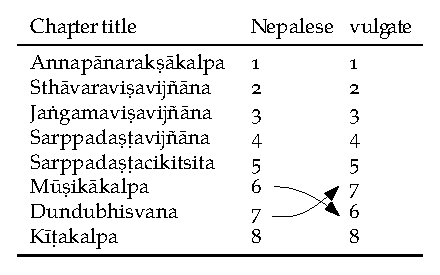
\includegraphics[width=0.65\linewidth]{chapters/media/kalpa}
%    \begin{tabular}{lll}
%    \emph{Chapter title} & \emph{Nepalese} & \emph{vulgate}   \\
%    \toprule
%      Annapānarakṣākalpa   &  1 &  1 \\
%     Sthāvaraviṣavijñāna & 2 &  2\\
%     Jaṅgamaviṣavijñāna &  3 & 3 \\
%     Sarppadaṣṭavijñāna & 4  &  4 \\
%     Sarppadaṣṭacikitsita & 5 & 5 \\
%     Mūṣikākalpa &  {6} & \textbf{7} \\
%     Dundubhisvana & {7} & \textbf{6} \\
%     Kīṭakalpa & 8 & 8 \\
%    \bottomrule  
%    \end{tabular}
\end{table}

% TODO: \usepackage{graphicx} required
%\begin{figure}
%    \centering
%    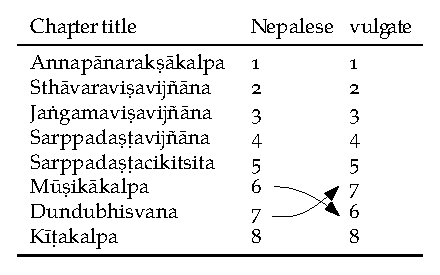
\includegraphics[width=0.65\linewidth]{chapters/media/kalpa}
%    \caption{}
%    \label{fig:kalpa}
%\end{figure}

\noindent
This difference in sequence does not have an immediately obvious 
significance.

\section{The Spread of Indian Toxicological Lore to Medieval Islamic 
Authors}

\citet[Introduction]{leve-1966} on 
\begin{itemize}
    \item tr. of the \SS\ under the Barmakids (Pramukhas) in 
    eighth-ninth-century Baghdad.
    \begin{quote}
        Much more important is the fact
        that Mankah is known as the translator of the Susruta
        samhita, a huge medical compendium, for Yahya b.
        Khalid. Ibn abi Usaibi'a (1203/4-1270) also discusses
        Mankah as an important Indian physician. Al-Jaiz
        (d. 868/9) knew of Mankah.'
        \ldots
        
        Yahya ibn Khalid, a Barmecide, was famous in his
        day in the field of science. In ibn al-Nadim, it is
        related that Yah.ya sent a scholar to India to study
        Indian drugs and religion, and brought Indian physi-
        cians and philosophers westward so that he might learn
        from them.
        Caliph al-Ma'mfin  also was interested in the sci-
        ences and so brought many scientists to his court from
        Jundishapfir where there were not only Greek men of
        science but also Indians who had brought their science
        and wisdom.
        \footnote{\cite[6]{leve-1966}}
    \end{quote}
    
    \item ibn Wahshiya's Book on Poisons (ca. 950). 
    \begin{quote}
        Not much is known of Shanaq himself. However,
        what is one of the earliest mentions of him is made in
        ibn Wahshiya's Book on Poisons (ca. 950). He refers
        to Shanaq's book as great and important. This state-
        ment is attested to by the fact that much of Shanaq's
        work was used by ibn Wahshiya. It was not, however,
        a base upon which the latter's work was built, as
        Strauss has claimed.
    \end{quote}
    \item The Poison book of Cāṇakya. 
\end{itemize}
            \thispagestyle{empty}
        % !TeX root = incremental_SS_Translation.tex
\chapter{Kalpasthāna 1: Protecting the King from Poison}

\section{Introduction}

\subsection{The meaning of “kalpa”}

What does “\emph{kalpa}” mean in the context of this section of the
\SS? In medical contexts, this polysemic term can mean an appropriate
drug recipe, a suitable medication, or any proper therapy.  The
present section of the \SS\ deals with poisonous herbs, animals and
insects, so one might expect the term to refer to antidotes or at
least drugs. However, the usage here points more to the sense
“procedure,” or “formal procedure,”  a sense that, in a secular context, 
echoes the
\emph{kalpa} of the \emph{Kalpasūtras}, the “formal procedures” of
Vedic ritual.\footnote{\citet[252]{wint-1981} translated \dev{kalpa}
    in the Vedic context simply as “ritual.”  He went on to describe the
    \emph{Kalpasūtras} as, “born out of the necessity to compile the
rules for
    the sacrificial ritual\ldots for the practical purposes of the
    priests.” \citet[467]{gond-1977} also used “ritual practice,” giving
    useful  further notes from classical authors in footnote~8.}
 %
%\label{arunadatta:kalpa}
%\emph{Sarvāṅgasundarī},
The twelfth-century author Aruṇadatta,\footnote{“A learned man with a great
command of a number of sciences,” \pvolcite{1A}[661]{meul-hist}.}
glossed \dev{kalpa} simply as \dev{prayogaḥ} “procedure”  and as
\dev{yojanam}.\footnote{\emph{Sarvāṅgasundarī} on \AH\
    \Ah{1.16.17ab}{246} and  \Ah{5.1 \emph{gadyasūtre 2}}{735}
    respectively.}


\subsection{Chapter 1 of the Kalpasthāna}
The first chapter of the Kalpasthāna of the \SS\
addresses the topic of protecting a king from those who would
assassinate him using poison. The king's kitchen is presented as the
site of greatest vulnerability.  The staff in the kitchen must be
vetted carefully and watched for signs of dissimulation.  The
description of the body-language that tells a poisoner (verses 18--25)
are engaging and vivid.  These verses are closely parallel in sense to
a passage in the \emph{Arthaśāstra} that says,
\begin{quote}
    The signs of a poisoner, on the other hand, are as follow: dry and
dark look on the face, stuttering speech, excessive perspiration
and yawning, trembling, stumbling, looking around while speaking,
agitation while working, and not remaining in his
place.\footnote{\emph{Arthaśāstra} 1.21.8 \citep[1,
    30]{kang-1969}, translation by \citet[97]{oliv-2013}.}
\end{quote}

Next, the text discusses the signs of poison in toothbrushes, in food, drink,
massage oil and other items that are likely to come into physical contact with the
king.  In passages that are again paralleled in the \emph{Arthaśāstra} the work
describes how poisoned food kills insects and crackles in a fire, flashing blue
and  the reactions of various birds to poison are described.\footnote{Cf.\
\emph{Arthaśāstra} 1.21.6, \emph{ibid.}, \citet[96]{oliv-2013}.}


The work then moves on to the various symptoms experienced by the king after 
being poisoned, and remedies appropriate to each case.  Poison exhibits 
characteristic signs when added to milk and other drinks.\footnote{Cf.\
\emph{Arthaśāstra} 1.21.6 again.} Further forms of poisoning, their symptoms 
and treatments are described  and finally the king is advised to live amongst 
trusted friends and to protect his heart by drinking various ghee compounds.  He 
should eat the meat and soup made from various animals, including peacock, 
mongoose, alligator, deer.  The chapter ends with the description of an emetic.

\section{Literature}

A brief survey of this chapter's contents and a detailed assessment of
the existing research on it to 2002 was provided by
Meulenbeld.\footcite[IA, 289--290]{meul-hist} Translations of this
chapter since Meulenbeld's listing have appeared by
\textcites[131--139]{wuja-2003}[3,
1--15]{shar-1999}{srik-2002}.\footnote{For a bibliography of translations
    to 2002, including Latin (1847), English (1877), Gujarati (1963) and
    Japanese (1971), see \cite[IB, 314--315]{meul-hist}. \citet{sing-1976} 
    translated this sthāna.}


\section{Manuscript notes}

\begin{itemize}
    \item \MScite{Kathmandu NAK 5-333} has foliation letter numerals, for example
on f.\,323a, that are similar to \MScite{Cambridge CUL 
Add.1693},\footnote{Scan
at 
\href{https://cudl.lib.cam.ac.uk/view/MS-ADD-01693/1}
{cudl.lib.cam.ac.uk/view/MS-ADD-01693/1}.}
 dated to 1165\,\CE.\footnote{See Bendall's chart of Nepalese 
 letter-numerals \citep[Lithograph V, 
after p.\,225]{bend-budd}.}
\end{itemize}

\newpage

\section{Translation}

\begin{translation}
 \item[1--2]  
 
 And now I shall explain the \se{kalpa}{formal procedure} for
safeguarding food and drink, as were declared by the Venerable
Dhanvantari.\footnote{MS H adds in the margin \dev{atha khalu vatsa
    suśrutaḥ} “Now begins Vatsa Suśruta.”  This phrase has been copied
    here by the scribe from the beginning of the \SS\ chapter in the
    \emph{sūtrasthāna} on the rules about food and drink
    (\Su{1.46.3}{214}).  The scribe presumably felt, not unreasonably,
    that this section had common subject matter with the present
    chapter.  Further, SS 1.46.3 is one of the few places in the
    Nepalese transmission of the \SS\ that names Dhanvantari and
    integrates him into the narrative of the \SS\ as the teacher of
    Suśruta. % Is Dh. the teacher of Su. elsewhere?
  
The mention of Dhanvantari here is one of the few times in the Nepalese
transmission that this authority is cited as the source of Ayurvedic
teaching, and the unique occurrence of this actual phrase, “as was
declared by the Venerable Dhanvantari.” See the discussion by
\citet[28--32]{kleb-2021b}, who concluded that the earliest
recoverable recension of the \SS\ may have had the phrase only at this
point and not elsewhere in the work. See the further discussion by
\citet{birc-2021}.  “Dhanvantari” is mentioned in the Nepalese version at 
1.1.21, 1.19.37, 1.46.3, 1.29.71, 1.34.1.1, 2.1.3, 2.7.3, 3.19.13.3, 4.2.3, (5.1.2, 
note), 5.4.3, 6.60.2, 6.64.84.%
}\q{Is Dh. the teacher of Su. elsewhere?}
 
 \item[3] 

 Divodāsa, the king of the earth, was the foremost supporter of religious
discipline and virtue. With unblemished instruction he taught his students, of
whom Suśruta was the leader.\footnote{This is a quite different statement from
the vulgate which has Dhanvantari as the teacher, and calls him the
\se{kāśipati}{Lord of Kāśī} \citep[559]{vulgate}.  Ḍalhaṇa followed the vulgate
but explicitly noted the reading before us with small differences: \dev{divodāsaḥ
kṣitipatistapodharmaśrutākaraḥ} “Divodāsa, the king of the earth, was a mine of
traditions about discipline and virtue.”}

\subsection{[Threats to the king]}

\item[4--5]  

Evil-hearted enemies who have plucked up their courage, may seek to harm the king,
who knows nothing of it.  He may be assailed with poisons by or by his own people
who have been subverted, wishing to pour the poison of their anger into any
vulnerability they can find.\footnote{Verses about the use of Venemous Virgins as a weapon
do not appear in the Nepalese manuscripts. Cf.\ \cite[81\,f., 132]{wuja-2003}.  This material 
is present in the commentary of Gayadāsa.} 

\item[6] Therefore, a king should always be protected from poison by a physician.

%A king may be cunningly assailed with poisons by evil-hearted enemies who
%have plucked up their courage, or even by his own people turned traitor,
%wishing to pour the poison of their anger into any chink they can find. Or
%sometimes by women using various concoctions, hoping to make him love
%them.\footnote{On how women of ill-character mix their nail-clippings or
%menstrual blood, etc.\ with the king's food, see
%p.\,\pageref{dusyodara}.} Or again, if a Venomous Virgin is used, a man can
%lose his life instantly.\label{visakanya}
%% \footnote{\label{visakanya}On the `Venomous
%% Virgin', see p.\,\pageref{intro:visakanya}.}

\item [7] 

The racehorse-like fickleness of men's minds is well known. And for this reason, a
king should never trust anyone.\footnote{The verb $\surd$ śvas is conjugated as a
first class root in the Nepalese manuscripts.}

\item [8--11]

He should employ a doctor in his \se{mahānasa}{kitchen} who is respected by experts, who 
belongs to a good family, is orthodox, sympathetic, not emaciated, and always busy.

\item [12--13]

The kitchen should be constructed at a recommended location and orientation.  It should
have a lot of light,\footnote{We read \dev{mahacchuciḥ} with the Nepalese manuscripts and 
against the vulgate's \dev{mahacchuci}.  We understand \dev{śucis} as a neuter noun 
meaning “light” following \citet[1050a]{apte-prac}.} have clean utensils and be staffed by 
men 
and
women who have been vetted.\footnote{Verses detailing the ideal staff are omitted in the 
Nepalese manuscripts. 
Cf.\ \cites[560]{vulgate}[132]{wuja-2003}.}


\item[17--18ab]

The chefs, \se{voḍhāra}{bearers}, and makers of boiled rice soups and cakes and whoever
else might be there, must all be under the strict control of the
doctor.\footnote{The word \dev{saupodanaikapūpika} “chefs for the boiled rice soups
and cakes” is grammatically interesting.  The term \dev{sūpodana} (as opposed to
\dev{sūpaudana}) is attested in the \emph{Bodhāyanīya\-gṛhyasūtra} 2.10.54 
\citep[68]{shas-1920}.  More pertinently, perhaps, \dev{sūpodana} is attested in
the Bower Manuscript, part II, leaf 11r, line 3 \citep[vol.\,1,
p.\,43]{hoer-bowe}.} 
% 2.11.54 supodana in the Bodh. (from Einoo's cards)
% sūpodana kṣīrodana
% Bower MS 328
% Kāty  otoṣthayoḥ samāse vā.

\item[18cd--19ab]

An expert  knows people's \se{iṅgita}{body language} 
through abnormalities
in voice, movement and facial expression. He should be able to identify 
a poisoner by the following signs.\q{Cf.\ Arthaśāstra 1.21.8.}


\item[19cd--23]

Wanting to speak, he gets confused, when asked a question, he never arrives at an
answer, and he talks a lot of confused nonsense, like a fool.  He laughs for no
reason, cracks his knuckles and scratches at the ground. He gets the shakes and
glances nervously from one person to another. His face is drained of colour, he is
\se{dhyāma}{grimy} and he cuts at things with his nails.\footnote{The word
\dev{dhyāma} is glossed by Ḍalhaṇa (in a variant reading) as someone who is the
colour of dirty clothes \Su{5.1}{560}.}  A poisoner goes the wrong way and is
absent-minded.

\item[25--27]

I shall explain the signs to look for in toothbrush twigs, in food and drink as
well as in \se{abhyaṅga}{massage oil} and \se{avalekhana}{combs}; in
\se{utsādana}{dry rubs} and showers, in \se{kaṣāya}{decoctions} and
\se{anulepana}{massage ointment}; in \se{sraj}{garlands}, clothes, beds, 
armour
and ornaments; in slippers and footstools, and on the backs of elephants and
horses; in \se{nasya}{snuff}, \se{dhūma}{inhaled smoke}, \se{añjana}{eye
    make-up}, etc., and any other things which are commonly poisoned. Then, I 
    shall
also explain the remedy.

\item[28]

% My old Susruta.tex translation has \bird and \animal commands for making 
% indexes.  Convert them to the \se{}{} command that we're using in the 
% present document.
\newcommand\animal[4]{\se{#2}{#1}} 
\let\bird=\animal 

%28
Flies or crows or other creatures that eat 
a poisonous \se{bali}{morsel} served 
from the king's portion, die on the spot. 

\item [29] 

Such food makes a fire crackle violently, and gives it an overpowering colour like
a peacock's throat.

\item[30--33]

%Its flames sputter, it has acrid smoke, and before long it goes out. 

After a chukar partridge %\animal{chukar partridge}{cakora}{Alectoris
% chukar}{Collins 45}
looks at food which has poison mingled with it, its eyes are promptly drained of
colour; a peacock pheasant %\animal{peacock pheasant}{jīvajīvaka}{Polyplectron
% bicalcaratum}{Dave BSL 270, 273,
%274, 281}
drops dead.  A koel %\animal{koel}{kokila}{Eudynamys scolopacea}{Collins 66}
changes its song and the common crane %\animal{common crane}{kroñca}{Grus
% grus}{Collins 47}
rises up excitedly.\footnote{The verb \dev{arcchati} “rises up” is a rare form
best known from epic Sanskrit \citep[see][212, \S 7.6.1]{ober-2003}.   The
transmitted form \dev{kroñca} is obviously a colloquial version of Sanskrit
\dev{krauñca}.  Commenting on \Su{1.7.10}{31}, Ḍalhaṇa interestingly gives the
colloquial versions of several Sanskrit bird names, even singling out
pronunciation in the specific location of Kānyakubja.  For \dev{krauñca} he says
that people pronounce it \dev{kurañja} and \dev{koṃci}.  The form \dev{koñca}
is found in Pāli (see \cite[731]{cone-dict}, who notes that Ardhamāgadhī has the
same form). Elsewhere, Ḍalhaṇa calls the bird \dev{krauñcira},  \dev{krauñci}, and 
\dev{kaicara}
(\Su{1.46.105}{223}, \Su{6.31.154}{684} and
(\Su{6.58.44}{790} respectively).}  It will excite a peacock 
%\bird{peacock}{mayūra}, %{Pavo cristatus}{Collins 39}
and the terrified parakeet %\saneng{parakeet}{śuka}%{Psittacula krameri\slash
% eupatria\slash
%cyanocephala}{Collins 64}
and the hill myna %\ssaneng{hill myna}{sārikā}%{Acridotheres tristis tristis, L.,
% etc.}{Ali \#1006,
%\citet[28\,ff.]{Dave}, \citet[119]{Collins}}
screech. The swan %\animal{swan}{haṃsa}{?}{?}
trembles very much, and the racket-tailed drongo %\animal{racket-tailed
% drongo}{bhṛṅgarāja}{Dicrurus paradiseus}{Collins 123}
churrs.\footnote{Ḍalhaṇa seemed confused about the \sed{bhṛṅgarāja}{racket-tailed
drongo}.  He called it a generic \sed{bhramaraka}{drongo}, a word that can also mean 
“bee,” \citep[62]{dave}, and then said that it is like the
\sed{dhūmyāṭa}{black drongo} \citep[for a nice explanation of this name,
see][62--63]{dave} and that people call it “the king of birds.”} The chital deer
%\saneng{pṛṣaṭa}{chital}  
sheds tears and the
monkey releases excrement.\footnote{\MScite{Kathmandu KL 699} reads 
“\sed{vṛṣabha}{bull}" for
“\sed{pṛṣata}{Chital deer}.”  The latter may perhaps be mistaken for the former in
the Newa script, although the reading of \MScite{Kathmandu KL 699} is hard to 
read at this point.}

\item[34cd]

Vapour\sse{bāṣpa}{vapour} rising from tainted food gives rise to a pain in the 
heart,
it makes the eyes roll, and it gives one a headache.\footnote{ “Tainted” translates
\dev{upakṣipta}.  The word's semantic field includes “to hurl, throw against,” and
especially “to insult verbally, insinuate, accuse.”  The commentator Ḍalhaṇa
glossed the term as, “spoiled food given to be eaten” (\dev{vidūṣitasyānnasya
bhoktuṃ dattasya}), but he noted that some people read “\dev{ukhākṣipta}” or
“thrown into a pan.”  Other translators have commonly translated it as “served,” perhaps
influenced by Ḍalhaṇa's “\sed{datta}{given}.”}


\item[35, 36cd] 

\diff{In such a case, an errhine and a collyrium that are costus,
    \gls{lāmajja}, \gls{nalada} and \se{madhus}{honey}};\footnote{The
    vulgate supplies another phrase and verb at this point that is not
    present in the Nepalese transmission, but that makes the text flow
    more easily.}  a paste of sandalwood on the heart may also provide
    relief.\footnote{\citet[350]{sing-1972a} discussed the difficulties
        in identifying \dev{lāmajja}, a plant cited more often in the \SS\
        than in the \CS; Ḍalhaṇa adopted the common view that it is a type of
        \emph{uśīra} or vetiver grass.  The grammatical neuter form
        \dev{madhus}  “sweetness” of the Nepalese manuscripts is less common
        than neuter \dev{madhu} “honey, sweetness, liquorice.”}

\item[37]

Held in the hand, it makes the hand burn, and the nails fall out. In such a case,
the \se{pralepa}{ointment} is \gls{śyāmā}, %{Callicarpa macrophylla,
% Vahl.}{AVS 1.334,    NK \#420},
\gls{indragopa}, %{Kerria lacca
% (Kerr.)}{http://www.icar.org.in/ilri/de fault.htm},
soma and \gls{utpala}.%
%{Nymphaea stellata, Willd.}{GJM 528, IGP 790; Dutt 110, NK \#1726}
\footnote{\label{beautyberry}“Beautyberry” (\emph{Callicarpa macrophylla} 
Vahl.) is one
identification of \dev{śyāmā}, but vaidyas and commentators have different ideas
about the plant's identity (see glossary).  
\par 
On translating \dev{indragopa} as “velvet-mite,”
see \cite{lien-1978}. Ḍalhaṇa's remarks show that he had a reading
\dev{indrāgopā} before him, and he tries to explain \dev{indrā} and \dev{gopā} as
separate plants.  But he also says that some people read \dev{indragopa}. 
\par
 Ḍalhaṇa
curiously parsed the name \dev{somā} (f.) out of the compound; this feminine noun
is almost unknown to Ayurvedic literature.  Some dictionaries and commentators
consider it a synonym for \dev{guḍūcī}, others for \dev{brāhmī} or
\dev{candrataru}.  Ḍalhaṇa also mentioned that some people think the word refers to
the \sed{somalatā}{soma creeper}, which might explain his choice to take the word as
feminine.  But the compounded word is far more likely to be \dev{soma} (m.), the
well-known mystery plant \citep[see][76--78, 125]{wuja-2003}.  If this can be
taken as rue (\emph{Ruta graveolens}, L.), as some assert, one can point to a
pleasing passage in Dioscorides where rue plays an antitoxic role: “\ldots it is a
counterpoison of serpents, the stinging of Scorpions, Bees, Hornets and Wasps; and
it is reported that if a man be anointed with the juice of the Rue, these will not
hurt him; and that the serpent is driven away at the smell thereof when it is
burned; insomuch that when the weasel is to fight with the serpent she armeth
herself by eating Rue, against the might of the serpent” \parencites[cited 
from][262]{wren-1956}[not found in][]{osba-dios}.}
     
     \item [38--39] If he eats that food, through inattention or by mistake,
then his tongue will feel like a \se{aṣṭhīlā}{pebble} and it will lose its
sense of taste. It stings and %\sskt{stings}{tudyate},
burns, and his \se{śleṣman}{saliva}\label{saliva} dribbles out.\footnote{The
    word \dev{aṣṭhīlā} is normally feminine.   The Nepalese manuscripts read it 
    with
    a short \dev{a-} ending.  Gayadāsa noticed that some manuscripts read
    \dev{aṣṭhīla} with a short \dev{-a} ending (\MScite{Bikaner RORI 5157},
    f.\,5v:7--8) and Ḍalhaṇa reproduced his observation.  The vulgate reading
    \dev{cāsyāt} “and from his mouth” is more obvious (\emph{lectio facilior}), 
    but
    is not attested in the Nepalese manuscripts.} In such a case, he should apply
    the treatment recommended above for \se{bāṣpa}{vapour}, and what will 
    be stated
    below under “toothbrush twigs”.\footnote{Poisoned toothbrushes are 
    discussed in
        verses 48\,ff.\ below.}
     
     \item[40]
     
     On reaching his stomach, it causes \se{mūrcchā}{stupor}, vomiting, the hair
stands on end, there is distension, a burning feeling and an impairment of
the senses.\footnote{I translate \dev{mūrcchā} in the light of the metaphors
discussed by \citet{meul-2011}, that include thickening and losing
consciousness.}

     \item[41] 
     
In this case, vomiting must quickly be induced using the fruits of
\gls{madana}, %{Randia dumetorum, Lamk.}{NK \#2091},
\gls{alābu}, %{Lagenaria vulgaris, Seringe.}{NK \#1419},
\gls{bimbī}, %{Coccinia indica, W. \& A.}{PVS 1994.4.715; NK 534}
and \gls{koṣītakī}, %{Luffa cylindrica, (L.) M. J. Roem.
% \textnormal{or}
% L. acutangula, (L.) Roxb.}{ADPS 252, NK \#1514 etc.}
taken with milk and \gls{udaśvit}, or alternatively with
rice-water.
     
     \item[42]
     
    
 Reaching the \se{pakvāśaya}{intestines}, it causes a burning feeling, stupor,
diarrhoea, thirst, impairment of the senses, \se{āṭopa}{flatulence} and it makes
him pallid and thin.
    
    % % % % % % % % % % % % % % % % % % % % %
    
      \item [43]
In such a case, purgation with the fruit of \se{nīlī}{indigo}, 
       %{Indigofera tinctoria, L.}{NK \#1309},
together with ghee, is best.  And  `\se{dūṣīviṣāri}{slow-acting poison antidote}'
should be drunk with honey and \se{dadhi}{curds}.\footnote{The `slow-acting
poison' is discussed at \Su{5.2.25\,ff.}{565}.}
     
     \item[44]
     
     When poison is in any liquid substances such as milk, wine or water, there are
     various streaks, and foam and bubbles form.  

     \item[45]
     
     \q{I'm still unhappy about this verse.} And no reflections are visible or,
however, if they can be seen once more, they are distorted, fractured, or
tenuous and distorted too.\footnote{Both Nepalese witnesses read
\dev{vikṛta} ({distorted}) twice, which is tautologous.  In the first occurrence
both read \dev{vikṛtā} without proper termination.  One might read the sandhi
in the second occurrence as \se{vāvikṛtā}{or not distorted}, but this gives
no better sense. The scribe of \MScite{Kathmandu NAK 5-333}, apparently the
original hand,  added in the margin the alternate reading
“\se{yamalā}{double}” as in the vulgate. Perhaps the scribe too was troubled
by the tautology.  It is also evidence that he was aware of a witness with
variant readings similar to the vulgate. We emend for grammar but retain the
\emph{lectio difficilior}.} \q{Mention this in the introduction as an example
    of the scribe knowing the vulgate.}
     
\item[46]

Vegetables, soups, food and meat are soggy and tasteless.  They seem to go stale
suddenly, and they have no aroma.\q{fn about sadyas+}  

\item[47] 

All edibles lack aroma, colour or taste.  Ripe fruits rapidly \se{pra$\surd$kuth}{rot} and 
unripe ones ripen.\footnote{The root $\surd$\dev{kuth} “stink, 
    putrify, rot” 
    is apparently known only from its few uses in the \SS.}

\item[48]

When a toothbrush twig has poison on it, the bristles are corroded and the
flesh of the tongue, gums and lips swells up.\footnote{Gayadāsa and Ḍalhaṇa 
pointed out that “\sed{dantaveṣṭa}{tooth socket}” and 
“\sed{dantamāṃsa}{gum}” have the same meaning 
(\Su{2.16.14--26}{331--332}).}

\item[49]

 Then, once his swelling is 
 lanced, one should \se{pratisāraṇa}{rub} it with
 \gls{dhātakī} flowers
 %{Woodfordia fruticosa (L.) Kurz}{AVS 5.412, NK \#2626}
 %{Terminalia chebula Retz.}{NK \#2451}, 
 \gls{jambū},
 %{Syzygium cumini, (L.) Skeels}{ADPS 188, NK \#967, Potter 168}
 \gls{āmra} stones and
 \gls{harītakī}
 fruit mixed with honey.\footnote{This recipe is different from the vulgate.}
 
 \item[50] Alternatively, the \se{pratisāraṇa}{rubbing} can be done with either
 the roots of \gls{aṅkolla}, the bark
of \gls{saptachada} or \gls{śirīṣamāṣaka}.\footnote{The 
    spelling of
the name \dev{aṅkolla} varies \dev{aṅkoṭa, aṅkoṭha, aṅkola} 
\citep[5]{gvdb};
Ḍalhaṇa noted that the form  \dev{aṅkolla} is a colloquialism
(\Su{1.37.12}{161}).  The sentence is awkward and we have emended
\dev{śirīṣamāṣaka} to be a plural, as in the vulgate, rather than the ablative 
singular of 
the Nepalese witnesses.  We follow Ḍalhaṇa in interpreting the compound to refer 
to the distinctive bean-like siris seeds, rather than to \gls{māṣaka} 
(\Su{5.1.50}{562}).}

\item[51ab] 
 
One should give advice about a poisoned tongue-scraper or 
\se{kavala}{mouthwash} in the
same way as  for a toothbrush twig.

\item[51cd]

Massage oil that has been laced with poison is slimy, thick and discoloured.   

\item[52]

When the massage oil has been contaminated with poison, boils arise,
pain, a \se{srāva}{discharge}, inflammation of the skin, and
sweating.\footnote{The feminine \dev{sphoṭā} for “boils” is unattested.}
    And the flesh splits open.

\item[53--54]

In such a case, sandalwood, \gls{tagara}, \gls{kuṣṭha}, and 
\gls{uśīra}, 
\gls{veṇupatrikā}, 
\gls{somavallī}
and 
\gls{amṛtā}, 
\gls{śvetā}, 
\gls{padma}, and 
\gls{kālīyaka} should be made into an
\se{anulepana}{ointment} for the patient, who has been sprinkled with cold 
water.
That is also recommended as a drink with the juice and leaves of
\gls{kapittha}.\footnote{This compound could be interpreted as 
“wood
apple juice and \gls{patra}.”  Note that this recipe is differs
from that of the vulgate, which requires urine.}
 
 \item[55]
 
In the case of a \se{utsādana}{dry rub}, a \se{parīṣeka}{shower}, an infusion, a
\se{anulepana}{massage ointment}, or in beds, clothes, or armour, the physician 
should understand that it is the same as for 
\se{abhyaṅga}{oil massage}.\footnote{See verse 52 above.}
 
 \item[56--58]
 
 When a comb has poison in it, the hair falls out, the head aches and blood
oozes from the \se{kha}{follicles} and \se{granthi}{lumps} appear on the
head. In such a case, one should repeatedly apply an ointment of black earth
soaked with \diff{bear's bile},\q{Bear's bile instead of deer's bile.}
\label{fluidbile}\footnote{Ḍalhaṇa comments here that `bile is that fluid
    which goes along inside the tube attached to the liver'
    (\dev{kālakhaṇḍa\-lagna\-nalikā\-madhya\-gata\-jalaṃ pittam})
    \Su{5.1.57}{562}.} ghee, \gls{śyāmā},\footnote{See note \ref{beautyberry}.}
        \gls{pālindī},
        and \gls{taṇḍulīyaka}.
        Good alternatives are either the fluid extract of cow-dung, or the juice of
        \gls{mālatī}, 
        the juice of \gls{mūṣikakarṇī},
        or household soot.\footnote{The plant identifications in this passage follow
            Ḍalhaṇa's glosses, although he noted a difference of opinion on the identity
            of \gls{mūṣikakarṇī} (lit.\ “mouse-ear”). \par The expression \dev{dhūmo
            vāgārasaṃjñitaḥ} `\ldots or the smoke termed ``house''\,' is commonly
            interpreted by translators and in Ayurvedic dictionaries as `household soot,'
            and this does seem to be the meaning, in context.  The term was
            comprehensively discussed by \citet[443]{meul-2008}. Cf.\ note
            \ref{grhadhuma}, p.\,\pageref{grhadhuma}.\label{soot}}
 
 
 \item[59]
 
 If either massage oil for the head, or a helmet for the head, in a wash, turban, or 
 garlands that are contaminated with poison, then one should treat it in the same 
 way as a comb.
 
 \item[60--61]
 
 When face make-up is poisoned, the face becomes dark and has  the symptoms 
 found
with poisoned massage oil. It is covered with \se{kaṇṭaka}{spots} that are like
\se{padminīkaṇṭaka}{lotus-spots}.\footnote{See the description of this condition
at \Su{2.13.40}{323}, where the skin on the face is characterized as having pale
circular patches that are itchy and have spots.}  In this case, the drink is
honey and ghee, and the \se{pralepa}{ointment} is sandalwood %{Santalum
%album, L.
% %}{ADPS 111, NK
%%\#2217}
with ghee, curds, honey, \gls{phañjī}, %{Clerodendrum
%serratum, L.}{AVS 2.121, ADPS 87},
\gls{bandhujīva} %{Pentapetes phoenicea, L.}{NK \#1836},
and \gls{punarnavā}.\footnote{The common plant-name 
\dev{punarnavā} is
read as \dev{punarṇṇavā} in both Nepalese witnesses.  This unusual form is
technically-speaking legal according to Pāṇini 8.4.3, but is not attested in
published texts.  \dev{punarṇavā} is found rarely in some other Nepalese
manuscripts such as the \emph{Brahmayāmala} (a.k.a.\ \emph{Picumata}, 44.81,
transcription thanks to Shaman Hatley), and elsewhere (e.g., in
\cite[20]{gana-1920}, where it is the name of a constellation.}\q{punarṇṇavā in
    the N \& K MSS} %{Boerhaavia
%diffusa, L.}{ADPS 387, AVS
%1.281,NK \#363}.
 
\item[62--63ab] 

Elephants and the like become ill and they dribble saliva. And the rider gets
\se{sphoṭa}{spots} and a discharge on his scrotum, penis, and rectum. In this
case, one prescribes the same therapy as for poisoned massage oil for both the
rider and the mount.

\item[63cd--65ab]

When there is poison in \se{nasya}{snuff} or smoke, the \se{liṅga}{symptom} is
blood coming out of the \se{kha}{apertures of the head}, a headache, a flow of
\se{kapha}{mucus} and impairment of the senses.

In such a case, 
ghee of cows etc., boiled up\q{śrita for śṛta} with their milk
and \gls{ativiṣā},
%{Aconitum heterophyllum, Wall. ex     Royle}{AVS 1.42, NK \#25},
is prescribed, with
%\se{śvetā}{white clitoria}
%{Clitoria ternatea, L.}{AVS 2.129, NK \#621}
\gls{madayantikā},
%{Lawsonia inermis, L.}{AVS 3.303, NK \#1448, Potter 151},
 as a cold drink or errhine.

\item[65cd--66]

Flowers lose their fragrance and colour, and wilt. On smelling them, he gets a
headache and his eyes fill with water.  In this case, the treatment is what was
proposed above for \se{bāṣpa}{vapour} and that which is traditional for face
make-up.


\item[67--68]

When it is in ear-oil, there is  degeneration in the ear, and painful swelling.
There is also a discharge from the ear and in such a case it needs to be
\se{pratipūraṇa}{irrigated} promptly with ghee and honey.  
\se{svarasa}{Extracted
    juice} of \gls{bahuputrā} and  very cold juice of
\gls{somavalka} are also  recommended as 
something good.\footnote{The syntax of the Nepalese version is slightly unclear, 
but the vulgate has smoothed out the difficulties.}\q{explain more}

%\se{Asparagus racemosus, Willd.}{wild asparagus}{bahuputrā}{ADPS 441, 
%AVS 1.218, NK \#264, IGP 103,
%    IMP 4.2499ff., Dymock 482ff.}
%\se{svarasa}{juice} and ghee, mixed with honey. Very cold
%\se{Acacia polyacantha, Willd.}{white cutch tree}{somavalka}{AVS 1.30, IGP
%    7, GJM 602, IMP 2.935; \emph{pace} NK \#1038} juice is another desirable
%remedy.

\item[69]


When poison is mixed in with \se{añjana}{eye make-up}, he gets tears and
\se{upadeha}{rheum}, with a burning feeling, pain, \se{dṛṣtivibhrama}{faulty
    vision}, and possibly even blindness.\footnote{The term translated as  “faulty
vision” could also mean “rolling eyes.” “Eye make-up” is normally made of  
\gls{añjana}.}

\item[70--71]

In this case, one must immediately drink ghee and have it also
in an \se{tarpaṇa}{eyewash} with
\gls{māgadha}.\q{Medical difference from Sharma.}
%\se{Piper longum, L.}{long pepper}{māgadha} {NK \#1928; but cf.\ AVS    
%3.245},
%
% \se{Jasminium auriculatum, Vahl.}{needle-flower 
%jasmine}{māgadha}{AVS
% 3.245, but cf.\ NK \#1928 etc.}
One should have an \se{añjana}{eye ointment} of the juice of
\gls{meṣaśṛṅga}
%{Gymnema sylvestre (Retz.) R. Br.}{AVS
%    3.107, NK \#1173}, 
and have the \se{niryāsa}{extract} of 
\gls{varuṇa},
%{Crataeva magna (Lour.)  DC.}{AVS 2.202; ADPS 500; cf.\, NK \#696}.
% synonym of Crataeva nurvala Buch. Ham. 
\gls{kapittha} and 
%{Limonia acidissima, L.}{AVS 3.327, NK \#1021}, 
\gls{meṣaśṛṅga}
%{Gymnema sylvestre (Retz.)
%    R. Br.}{AVS 3.107, NK \#1173}, 
and the flower of 
\gls{bhallātaka}.\q{example where the vulgate clarifies that 
these should be used separately; appears to be a gloss inserted into the vulgate 
text.}
%{Semecarpus anacarium, L.}{NK\#2269, AVS 5.98},

\item[72--73]

Because of poisoned slippers there will definitely be a
swelling, \se{svāpa}{numbness}, a \se{srāva}{discharge} and an
outbreak of \se{sphoṭa}{spots} on the feet. One should \se{pra$\surd$
sādh}{clean} footstools together with slippers.

\item[74]

Ornaments lose their lustre, and they do not shine as they used to.
They damage their respective locations with  burning, 
\se{pāka}{sepsis}, and \se{avadāraṇa}{fissuring}.\footnote{The reading 
\dev{avadāruṇa} in MS Kathmandu KL 699 is not attested elsewhere in Sanskrit 
literature.  On “sepsis” for \dev{pāka}, see \cite[xlv--xlvi]{wuja-2003}.}

\item[75ab]

One should apply the stated procedure for \se{abhyaṅga}{massage oil} to
poisoned slippers and ornaments.

\item[75cd--76]  In the case of the \se{upasarga}{affliction} by
poison which has been described above, starting from `vapour' and
ending with `ornaments,' the physician should observe the
\se{upadrava}{side-effects} and then prescribe the therapy called the
\se{mahāsugandha}{Great Fragrance} antidote,  which I shall
describe.\footnote{This antidote is indeed described later, in
    dramatic terms, at \Su{5.6.14--27}{581}.  A recipe with eighty-five
    ingredients including cow's bile, it is praised as chief of all
    antidotes, one that can drag the patient back from the very jaws of
    death, from even the poisonous fangs of Vāsuki. A useful survery of the 
    meanings of \dev{upsarga} (“affliction”) was given by 
    \volcite{IB}[332]{meul-hist}}


% got to here

\item [77--78ab] He should prescribe it in drinks, \se{ālepana}{liniments},
\se{nasya}{errhines}, and in \se{añjana}{eye ointment}.  Also, he should use 
sharp
purgatives and emetics.  If bleeding is present, he should have the
indicated\q{The two uses of prāpta are hard to translate.  prāptāḥ $\rightarrow$
    kṣipraṃ is an example of the vulgate banalizing the Sanskrit text to make 
    sense of
    a difficult passage.} veins pierced.\q{$\surd$ vyadh not $\surd$ vedh (also elsewhere
    and for the ears), causative optative.}


\item[78cd--79ab]

If either \gls{mūṣikā} %{Jatropha curcas, L.}{AVS 3.261, NK
%\#1374}
or a \gls{ajaruhā} is tied on to the King's wrist, then all food that is mixed
with poison will be rendered free of poison.\footnote{In early Ayurvedic
    literature, the plant \dev{ajaruhā} is mentioned only here and its identity is
    unknown.  It may be a fern of the Nephrodium family, according to
    \citet[7]{gvdb}.  Ḍalhaṇa, on \Su{5.1.78}{563}, cited a description of the two
    plants from the little-known authority Uśanas \citep[IA, 660 et
    passim]{meul-hist} who described \dev{ajaruhā} as a white root with spots on
    it that looks like collyrium when it is split; when drunk with sandalwood it
    causes poison to be digested.}

%\emph{kandaḥ śvetaḥ
% sapiḍako bhede
% cāñcanasannibhaḥ/ gandhalepanapānais
%tu viṣaṃ jarayete nṛṇām//}

\item[79cd--80]

He should always guard his heart when amongst \diff{people who are not
    his friends}.\footnote{The \emph{Carakasaṃhitā} described “protecting the
    heart” (\dev{hṛdayāvaraṇa}) as drinking several sweet, oily drinks to
    surround the heart and keep it safe (\Ca{6.23.46}{574}).
    \Dalhana{5.1.79--81}{563} explained it as taking a number of anti-toxic
    medicines, including those listed in the present passage, in order to
    cover or hide (\dev{pracchādana}) the heart.  Note that the Nepalese
    version reads the opposite of the vulgate: one should guard one's heart
    when amongst enemies, not friends.  This is far more logical; it is also
    the reading known to the \As{1.8.89}{79}.} Before eating, he should drink
    the kinds of ghee called \sse{ajeya}{Invincible}\sse{amṛta}{Immortal}
    “Invincible” and “Immortal”.\footnote{These ghee compounds are described
        in later chapters: see \Su{5.2.47--49}{566} and \Su{5.6.13}{581}.} He
        should drink \se{sarpiṣ}{ghee}, \gls{kṣaudra}, \se{dadhi}{curds},
        \se{payas}{milk}, or cold water.


\item[81]

He should consume monitor lizard, peacock, \gls{nakula}, \gls{pṛṣata},
and \gls{hariṇa} too, that destroy poison, and their juices.

\item [82]

As discerning person should add well-crushed
\gls{pālindī},\footnote{\Dalhana{5.1.82}{563} equated this with
    \gls{trivṛt}.} \gls{madhuka}, and sugar to the meats of \gls{godhā},
    \gls{nakula} and \gls{hariṇa} too. 
\item[83]

Add sugar and \gls{ativiṣā} to peacock flesh, together with
\gls{mahauṣadha}. And for meat from a \gls{pṛṣata}, he should add
\gls{pippalī}, with \gls{mahauṣadha}.

\item[84ab]
\diff{A cold neem} broth with honey and ghee is wholesome too. 

\item [84cd]

A discerning person should partake of hard and soft foods that counteract
poison.\footnote{On this expression, see \cite{yagi-1994}.}
    
\item [85]

If poison might have been drunk, a person who has protected his heart
should make himself vomit using \gls{pippalī}, \gls{madhuka},
\gls{kṣaudra}, \gls{śarkara}, \gls{ikṣu} juice, and water.

\bigskip

The first chapter in the Kalpas. 

    \end{translation}

   
   


            \thispagestyle{empty}
        % !TeX root = incremental_SS_Translation.tex
\newcommand{\plant}[4]{#1 (\emph{#2})\footnoteA{#3; see #4}}
\let\chemical = \plant
\newcommand{\skt}[2]{#1 (\emph{#2})}
\newcommand{\sskt}[2]{\empty}
%

\chapter{Kalpasthāna 2: Poisonous Plants}

\section{Introduction}

This section begins with several lists of poisonous plants.  The
Sanskrit names for these plants are mostly not standard or familiar
from anywhere in Sanskrit or ethnobotanical literature.  It remains a
historical puzzle why these particular names are so difficult to
interpret. However, we are not the first to encounter these
difficulties. 

In the eleventh century, Cakrapāṇidatta commentated on 
a similar list of poisons in the \CS, and referred to the \SS\ on the 
topic.\footnote{\Cakra{6.23.11}{571}.}   He 
also noted that,
\begin{quote}
    In assigning the names to these plants, the main authorities are
the Kirātas and Śabaras, who know about these things because they
can explain these matters on the basis of a succession of
teachers.\footnote{Cakrapāṇidatta on \CS\ \Su{6.23.11}{571}.}
\end{quote}
\par
\noindent
About a century later, the learned commentator on the \SS, Ḍalhaṇa, 
remarked,
\begin{quote}
    \label{kiratas}
In spite of having made the greatest effort, it has been impossible to
identify these plants. In the Himalayan regions, Kirātas and Śabaras
are able to identify them.\footnote{After \SS, \emph{kalpasthāna} 2.5
    \citep[564]{vulgate}.}
\end{quote}
From the view of Sanskrit authors, Kirātas and Śabaras were tribal
peoples.\footnote{Both communities are mentioned in Sanskrit
    literature from antiquity.  The Kirātas are associated especially with
    Eastern Nepal, the Himalayan and north-eastern regions of South Asia,
    while the Śabara people are mainly associated with Odisha and West
    Bengal.  Representative studies on these communities include
    \citet{chat-1951,sing-2008,roy-1970,elwi-1955,subb-1999,rai-2019a,sing-1990}.}
     
In the tenth or eleventh century, the author Bhikṣu Govinda cast his
alchemical treatise as a dialogue with a Kirāta king called Madana who
was a master of the alchemical art.\footcite[IIA, 620]{meul-hist}  So
there was an awareness amongst Sanskrit medical and alchemical authors
of that period that different populations were a source of specialized
knowledge in these domains, and the Sanskrit authors were open to
these sources and indeed depended on them.

Ḍalhaṇa also recorded variant readings of these poison names from the
manuscripts that he consulted of the lost commentary of Gayadāsa
(fl.\,c.\,\AD\ 1000). The identities of these poisons have thus been
in doubt for at least a thousand years.\footnote{See
    \cite[80--81]{wuja-2003}.} Firm identification has in many cases been
    equally impossible for us today.

One path for exploration in this situation is to attempt to
reverse-engineer some identifications by considering the known toxic
plants of India.\footnote{Valuable reference sources on Indian plant
    toxicology in general include \cite[chs.\,10, 11]{pill-2013} and
    \cite[parts 1.II, 3 and 4]{barc-2008}. More generally \citet[41 et
    passim]{bown-2001} comments usefully of herbs in general that “it
    goes without saying that if they can do good, they must contain
    substances that in excess can poison.”  See for a general list of poisonous 
    plants, see \cite{wiki-2025a}.}

%\section{Manuscript notes}
\subsection{Shock}

An important new topic introduced in this chapter (34--39) is that of “toxic
shock” (\emph{vega}).\sse{vega}{toxic shock}  When a patient has been 
poisoned, the effect of the toxin is expressed in their body in seven waves or 
pulses, \emph{vegas}.  At each stage, symptoms are slightly different and a 
different therapeutic regime is prescribed (40--44).  

The Sanskrit term \emph{vega} has a range of uses, from “impulse” to
“urge, jerk, rush, speed,” or “impetus.”  It appears in the
well-known passage in the \CS\ about avoiding illness not ignoring 
or suppressing “natural urges,” \emph{vegas}, such
as the desire to urinate.\footnote{See \CS\ \Ca{1.7}{49--55}, discussed and
    translated in \cite[7--8, 15--17]{wuja-2003}.}
    
According to the author of the \AS, Ālambāyana\label{alambayana1} was
the ancient authority who declared that the seven \se{vega}{pulses}
of toxic shocks affect, successively, the seven
\se{āśraya}{substrata} of the body, from blood to semen, and
Dhanvantari originated the idea that this applied to victims of
snake-bite.\footnote{\AS\ \As{6.40.35}{844}: \dev{sapteti vegā
    mūrchādyā videhapatinā smṛtāḥ//34// raktamāṃsavasāsnāyu
    tathā'sthyādyāstrayaḥ kramāt/ āśrayāḥ sapta
    saptānāmityālambāyano'bravīt//35//}.  The following verse named
    Dhanvantari as the originator of the idea that toxic pulses are
    experienced specifically by a person bitten by a snake 
    (\dev{vegāndhanvantaristadvatsarpadaṣṭasya manyate/} 36ab).  The
    commentator Indu noted that Dhanvantari was the teacher of Suśruta, i.e., 
    that “Dhanvantari" was shorthand for \SS.    
    On Ālambāyana, see p.\,\pageref{alambayana2}, note \ref{alambayana2}.}
    
The commentator Indu (fl.\,1000--1150) cited verses by Ālambāyana
asserting that the pipes in the body carry poison to the heart, but
that the heart can be protected by ghee. \footnote{\AS\ \As{6.40.60}{}:
    \dev{yāḥ sirāḥ sarvagātreṣu hṛdaye sampratiṣṭhitāḥ| tābhirasya viṣaṃ
    sarvaṃ hṛdayaṃ sampradhāvati// ghṛtena tu praticchannaṃ viṣaṃ nāti
    prapīḍayet/ nirvāṇajananaṃ sarpiḥ prāṇināṃ prāṇavarddhanam//
    hṛdayāvaraṇāstadvadbhakṣyā bhojyāśca sāgadāḥ//}}


\subsection{Literature}

Meulenbeld offered an annotated overview of this chapter and a bibliography
of earlier scholarship to 2002.\fvolcite{IA}[290--291]{meul-hist} 

\newpage

\section{Translation}

\begin{translation}
    
\item[1]

And now I shall explain \diff{\se{vijñānīya}{required knowledge}}
about stationary poisons.\footnote{No reference is made to
    Dhanvantari \citep[see][]{birc-2021}. “Stationary” here is a term
    contrasted with “moving,” and signifies plants as opposed to animals
    and insects.}
  
    \item[3]
    \noindent It is said that there are two kinds of poisons,
    \se{sthāvara}{stationary} and \se{jaṅgama}{mobile}. The former
    dwells in ten sites, the latter in sixteen places.
   
    \item[4]
    Traditionally, the ten are: root, leaf, fruit, flower, bark,
    \se{kṣīra}{milky sap}, \se{sāra}{pith}, \se{niryāsa}{resin}, 
    \sepl{dhātu}{mineral}, and the tuber.

    \item[5]
    
    In that context,\label{poisonousplants}
    \begin{itemize}
        \item[A] The eight items with poisonous roots are:\footnote{Some South 
        Asian
    plants with poisonous roots that we would expect to see in
    this list include \emph{Croton tiglium}, L., \emph{Calotropis}
    spp. (\egls{arka}, etc.), \emph{Citrullus colocynthus} L. Schrad. 
    (\egls{indravāruṇī}), and
    \emph{Ricinus communis} L. (\egls{eraṇḍa}), \citep{pill-2010}.} %
    % \q{Expected \citep{pill-2010}:\\ Croton
    %        tiglium, L. = Naepala, Jayapala, kanakaphala,
    % titteriphala
    % (NL \#720);
    %        Calotropis spp.;\\ Citrullus colocynthus (colocynth);\\
    % Ricinus communis
    %        (castor); }
        \begin{enumerate}
            
        \item  \gls{klītaka},\footnote{Liquorice eaten in excess can
    be poisonous, but it is uncertain whether it is the plant intended
    here.  \citet[124]{gvdb} specifically noted that the poisonous root
    mentioned in this passage, “remains to be identified.” Cf.\ glossary for 
    discussion.}
       
        \item \gls{aśvamāraka},
    
        \item \gls{guñjā},
        
        \item \diff{\gls{subhaṅgurā}},\footnote{The vulgate reads 
      \egls{sugandhā}, which can be poisonous.}
        
       \item \diff{\gls{karaṭā}},\footnote{Conjectural identification with 
       \emph{karahāṭa}; similar-sounding candidates also include 
       \egls{karkaṭaka} and \egls{karaghāṭa}, but since this is a prose passage, 
       there would be no reason to alter the word to fit a metre.} and ending with 
           
\item \gls{vidyutśikhā},

\item \diff{\gls{ananta-poison}},\footnote{\label{ananta-poison}The
    text reads masculine \emph{ananta}, which is not a plant name.  Gayī's
    commentary on \Su{5.2.5}{564} noted a variant reading of feminine
    \emph{anantā} in place of \emph{gargaraka}, earlier in the compound.
    But the feminine \egls{anantā} is not a poisonous
    plant.} and

% got to here 

\item \gls{vijayā-poison},\footnote{\citet[61, n.\,3]{meul-sear} argued that
    our text reads a masculine or neuter noun \emph{vijaya}, which never
    signifies cannabis. However, unlike the vulgate, the unanimous
    readings of the Nepalese manuscripts give feminine \emph{vijayā}. 
    Nevertheless, even the feminine form only started to signify
    \emph{Cannabis sativa} L. after the end of the first millennium
    \citep{meul-sear,wuja-cann,mchu-2021}. The \emph{Sauśrutanighaṇṭu}
    gives a number of synonyms for \emph{vijayā}, almost none of which
    have any poisonous parts \citep[5.77, 10.143]{suve-2000}.  But one of
    them, \emph{viṣāṇī} (also \emph{meṣaśṛṅgī}), is sometimes equated with
    \emph{Dolichandrone falcata (DC.) Seemann} \citep[518]{adps}, a plant
    used as an abortifacient and fish poison \citep[\#862]{NK}.  This
    identification is tenuous.} %
    %        \footnote{Large doses of the root-extract of rauwolfia
    % can be fatal.
    %
    %        In large doses luffa is emetic and a drastic purgative. }
        \end{enumerate}
        \end{itemize}
    
    
    % 5.2.5B
    
        \item[B]
        the leaf-poisons include:
             \begin{itemize}            
        \item \gls{viṣapatrikā},
        \item \diff{\gls{lambaradā}},
%        \item \plant{`choice tree'}{varadāru}{unknown}{?},
        \item \gls{karambha},
        and
        \item big \gls{karambha};
            \end{itemize}
% 5.2.5C
        \item[C]
        the fruits of items like:
        \gls{guñjā},
        \gls{aruṣkara},
        and
        \gls{viṣavedikā}
        are
\begin{itemize}
         \item \diff{\gls{kumudavatī}},	
        \item \diff{\gls{reṇukā}},
    \item \diff{\gls{kuruvaka}},
    \item \diff{\gls{veṇuka}},
    \item \gls{karambha}
    \item \gls{mahākarambha}
    \item \diff{\gls{nandanā}},
    \item \diff{\gls{kāka2}},
\end{itemize}
   
 % 5.2.5D 
        \item[D]
        the flower-poisons include those of:
\begin{itemize}
 \item \diff{\gls{ullika}}, 
 \item \diff{\gls{reṇu}},\footnote{\dev{reṇu} and \dev{reṇuka/kā} are 
 different plants. MS K reads the first; the scribe of MS H added an additional 
 \dev{-ka} in the margin.}
%        \item \gls{vetra},
%        \item \gls{kādamba},        
%        \item \gls{vallīja},
        \item \gls{karambha},
        and
        \item \gls{mahākarambha}.
\end{itemize}

% 5.2.5E        
        \item[E]
        the bark, \se{sāra}{pith} and \se{niryāsa}{resin} of:
\begin{itemize}
        \item \diff{\gls{vallija}},
%        \item \gls{kartarīya},
%        \item \gls{saurīyaka},
        \item \gls{karaghāṭaka},
        \item \gls{karambha},
%        \item \gls{nandanā},
        and
        \item \gls{nārācaka};
            \end{itemize}
 
 % 5.2.5F
        \item[F]
        the  \se{kṣīra}{milky sap} of:
              \begin{itemize}
            % got to here.  2024-09-27
        \item \gls{kumudavati},\footnote{While the identity of this plant is 
            uncertain, the Nepalese version of the \SS\ does not present the 
            hopeless problem of the vulgate's reading \dev{kumudaghnī}.}
%        \plant{purple calotropis}{kumudaghnī $\rightarrow$ arka?}{Calotropis
%            gigantea, (L.) R. Br.}{ADPS 52, AVS 1.341, NK \#427, Potter
%            63},\footnote{The name of this poison, \emph{kumuda-ghnī}, means 
%            `lotus
%        killer'.  In Sanskrit literature, the \emph{kumuda} lotus is associated
%        with the moon, since it blossoms by night.  Since the sun causes this 
%lotus
%        to close, it is therefore an `enemy' of the lotus.  One of the chief words
%        for the sun, \emph{arka}, is also the name of \emph{Calotropis 
%gigantea},
%        which indeed has a milky juice which is a violent purgative, poison and
%        abortifacient.}
%
\item \gls{dantī},
\item \gls{snuhā},
%        \item \plant{oleander spurge}{snuhī}{Euphorbia neriifolia, L., 
%        \textnormal{or}
%            E. antiquorum, L.}{ADPS 448, AVS (2.388), 3.1, NK
%            \#988, IGP 457b},
        %   \marginpar{`The milky juice or gum which flows from the branches
        %     [of \emph{E. antiquorum}] is an acrid irritant\ldots. Internally it is a
        %     powerful emetic and a violent purgative, even in very small quantities'.
        %     --- NK \#982}
and
\item \gls{jālinī}        
%        and 
%        \item \plant{`web-milk'}{jālakṣīri}{unknown}{?};
            \end{itemize}

% 5.2.5G        
        \item[G]
        the  \se{dhātu}{mineral} poisons include:\footnote{These identifications
            are more than usually uncertain.  Note that the vulgate
            text specifies that there are two mineral poisons.}
              \begin{itemize}
\item \gls{haritāla},
\item \gls{phenāśma}, 
\item \gls{bhasma}, and
\item \gls{rakta}.\footnote{If this identification as \egls{rakta} (cinnabar) is 
correct, it is an unexpectedly early mention of the substance.}        
%        \item \plant{`foam-stone'}{phenāśma}{unknown}{?}, and
%        \item \plant{orpiment}{haritāla}{Arsenii trisulphidum}{NK v.\,2,
%            p.\,20\,ff.};\footnote{\citet[38--42]{dutt-1922} conjectured that
%        `foam-stone' may be impure white arsenic obtained by roasting 
%orpiment.}
            \end{itemize}

% 5.2.5H        

% got to here.
        \item[H]
        the tubers poisons are:
        \begin{itemize}
             \item \gls{kālakūṭā},
%        The \emph{Rāja\-nighaṇṭu\-pariśiṣṭa} (9.35) gives \emph{kālakūṭaka} 
% as a synonym for \emph{kāras\-kara}, or \emph{Strychnos nux-vomica}, L., 
%        whose seeds are notoriously poisonous.}
\item \gls{vatsanābha},
%        \item \plant{wolfsbane}{vatsanābha}{Aconitum napellus, L.}{AVS 1.47,
%            NK \#42, Potter 4\,f.},
\item \gls{sarṣapa},
%        \item \plant{Indian mustard}{sarṣapa}{Brassica juncea, Czern. \&
%            Coss.}{AVS 1.301, NK \#378},
\item \gls{pālaka},
%        \item \plant{leadwort}{pālaka $\rightarrow$  citraka}{Plumbago 
%zeylanica
%            (indica? rosea?), L.}{Rā. 6.124, ADPS 119, NK \#1966,
%            1967},
\item \gls{kardama},
%        \item \plant{`muddy'}{kardama}{unknown}{?}, the
\item \gls{vairāṭaka},
%        \item \plant{`Virāṭa's plant'}{vairāṭaka}{unknown}{?},
\item \gls{mustaka},
%        \item \plant{nutgrass}{mustaka}{Cyperus rotundus, L.}{ADPS 316,
%            AVS 2.296, NK \#782},
\item \gls{śṛṅgīviṣa},
%        \item \plant{atis root}{śṛṅgīviṣa}{Aconitum heterophyllum, Wall.
%            ex Royle}{AVS 1.42, NK \#39},
        % \item \plant{liquorice}{prapuṇḍarīka $\rightarrow$ 
        %madhuka?}{Glycyrrhiza
        %  glabra, L.}{AVS 3.84, NK \#1136},\footnote{Non-toxic.}
\item \gls{prapauṇḍarīka},
%        \item \plant{sacred lotus}{prapuṇḍarīka}{Nelumbo nucifera, 
%        Gaertn.}{Dutt 
%        110, 
%        NK
%            \#1698}, 
\item \gls{mūlaka},
%\item \plant{radish}{mūlaka}{Raphanus sativus, L.}{NK 
%            \#2098},
\item \gls{hālāhala},
%        \item \plant{`alas, alas'}{hālāhala}{unknown}{Cf. Soḍhalanighantu 
%p.43 
%        (sub
%            bola) = stomaka = vatsanābha}, 
\item \gls{mahāviṣa},
%\item \plant{`big poison'}{mahāviṣa}{unknown}{?}, 
and 
\item \gls{karkaṭa}
%            \plant{galls}{karkaṭa}{Rhus
%            succedanea, L.}{NK \#2136}.\footnote{Leadwort root is a powerful 
%poison.
%        Nutgrass is tuberous, but non-toxic. Atis has highly toxic tuberous
%        roots. Neither sacred lotus nor galls are toxic. The `alas, alas' poison
%        (\emph{hālāhala}) is the mythical poison produced from the churning of
%        the ocean at the time of creation: it occurs in medical texts such as
%        the present one, and commentators identify it with one or other of the
%        lethal poisons such as wolfsbane or jequirity.
%        \citet[126]{agra-indi} makes the intriguing suggestion
%        that the word \emph{hālāhala},
%        possibly to be identified with Pāṇini's \emph{hailihila} (P.6.2.38),
%        may be of Semitic origin, although his evidence
%        seems uncertain (\citet[1506a]{stei-pers} cites Persian \emph{halāhil}
	%        `deadly (poison)' as a loan from Sanskrit). 
	% \volcite{iii}[585]{KEWA}
%        also cites a claim for an Austro-Asiatic origin for the word.}
            \end{itemize}


    
\subsection{The effects of poisons}

\subsubsection{Symptoms of root poisoning}
    \item[7--10]
    
People should know that root-poisons cause \se{udveṣṭana}{writhing},
\se{pralāpa}{ranting}, and \se{moha}{delirium}, and  leaf-poisons
cause yawning, writhing, and \se{śvāsa}{wheezing}.
    
 Fruit-poisons cause swelling of the
   scrotum, a burning feeling and writhing.  Flower-poisons will
    cause vomiting, \se{ādhmāna}{distension} and \se{svāpa}{sleep}.  
    
The consumption of poisons from bark, \se{sāra}{pith} and
\se{niryāsa}{resin} will cause foul breath, \se{pāruṣya}{hoarseness},
a headache, and a discharge of \se{kapha}{phlegm}.\footnote{At
    \Su{1.2.6 }{11}, Ḍalhaṇa glossed \se{pāruṣya}{hoarseness} as
    \emph{vāgrūkṣatā}, “a rough, dry voice.”}
    
    % 10
    
The \se{kṣīra}{milky sap}-poisons make one froth at the mouth,  cause
loose stool, and make the tongue feel heavy.\footnote{At
    \Su{6.54.10}{773}, Ḍalhaṇa glossed \se{viḍbheda}{loose stool} as
    \emph{dravapurīṣatā}, “having liquid stool.” }  The
    \se{dhātu}{element}-poisons give one a crushing pain in the chest,
    make one faint and cause a burning feeling on the palate.
    
    % 11
    These poisons
    are classified as ones which are generally speaking lethal after a period of time.
    
    \item[11--17]
    
    \subsubsection{Symptoms of tuber poisoning} The tuber-poisons,
though, are severe.  I shall talk about them in
detail.\footnote{See Ḍalhaṇa's comments on the impossibility of
    identifying the following plants, p.\,\pageref{kiratas} above. 
    All the following plant identifications are tentative in the
    extreme; see the glossary for discussion.}
    
    %12
    
    With
    \gls{kālakūṭa},
%    {kālakūṭa}{Abrus precatorius, L.?
%        Cf.\ RRS 21.14.}{AVS 1.10, NK \#6, Potter 168.},
 there is numbness and very severe trembling.

%
    With
    \gls{vatsanābha},
%    {Aconitum napellus, L.}{AVS 1.47,
%        NK \#38, Potter 4\,f.}, 
there is rigidity of the neck, and the faeces,
    and urine become yellow.
    
    %13
With \gls{sārṣapa}, 
%With \plant{Indian mustard
% roots}{sārṣapa}{Brassica juncāea, Czern \&
%    Coss.}{AVS 1.301, NK \#378}
the \skt{wind becomes defective}{vātavaiguṇya}, there is
\se{ānāha}{constipation}, and \se{granthi}{lumps} start to appear.

With \gls{pālaka}, % $\rightarrow$  citraka}{Plumbago zeylanica
%    (indica? rosea?), L.}{Rā. 6.124, ADPS 119, NK \#1966, 1967},
there is weakness in the neck, and speech gets jumbled.\footnote{The
    verse in the Nepalese version ends with a plural verb that does not
    agree with the dual of the sentence subject.}
    
    %14
With the one called \gls{kardama}, there is a
\se{praseka}{discharge}, the faeces pour out, and  the eyes turn
yellow. 

The \egls{vairāṭaka} causes pain in
the body and illness in the head. 

Paralysis of one's arms and legs and trembling are said to be
caused by \gls{mustaka}.%
%    \plant{nutgrass}{mustaka}{Cyperus rotundus, L.}{ADPS 316, AVS
% 2.296,
%        NK \#782} %
\footnote{The substitution in \MScite{NAK 5-333} affecting 15cd is
    caused by an eye-skip to the word \emph{viṣeṇa} in 2.17. 
    
    \emph{Mustaka} commonly refers to Cyperus rotundus, L.; the root is
    used in āyurveda but is not poisonous.  However other dictionaries
    list \emph{mustaka} amongst serious poisons, for example
    \emph{Rājanighaṇṭu} (22 v.\,42) and \emph{Rasaratnasamuccaya} 16,
    v.\,80.  However, its ancient identity is still doubtful.} 

\item[15b] 
% got to here
With \gls{mahāviṣa}, one's limbs grow weak, there is a burning feeling
and swelling of the belly.\footnote{The poisonous root \egls{mahāviṣa}
    is not clearly identifiable, although \emph{viṣā} is commonly aconite.
    Verse 6 above notes that there are several kinds of aconite.}
        
\item[16a] With \gls{puṇḍarīka},  
        %   \plant{sacred lotus}{puṇḍarīka}{Nelumbo nucifera,
        % Gaertn.}{Dutt 110,
        %        NK \#1698},
        one's eyes go red, and one's belly becomes
        distended.\footnote{The word \emph{puṇḍarīka} very commonly means
            white lotus. The entire plant is
            edible and cannot be the poison intended here. \citet[252]{gvdb}
            noted that this poison is unidentified and that it is also listed
            as a poison in \Cs{ci.23.12}{}.}\q{Look up the ca. reference.}

\item[16b] With \gls{mūlaka},    
            % \plant{radish}{mūlaka}{Raphanus sativus, L.}{NK \#2098}es,
            one's body is drained of colour and the limbs are
            paralysed.\footnote{The word \emph{mūlaka} very commonly means
                the radish, \emph{Raphanus sativus}, L. The root is edible and
                cannot be the poison intended here. \citet[317]{gvdb} noted that
                this poison is unidentified.}
    
    %17
    \item[17a]
        
    With \gls{hālāhala}, a man turns a \se{dhyāma}{dark colour}, and
gasps.\footnote{Identification of \emph{hālāhala} is  uncertain. It may simply
be a mythical poison, or its specific identity may have been lost over the
centuries. Late \emph{nighaṇṭu}s identify it as \emph{stomaka} =
\emph{vatsanābha}, i.e., \emph{Aconitum napellus}, L. 
(\emph{Soḍhalanighaṇṭu} p.\,43). 

Ḍalhaṇa on \Su{5.2.17}{564} interpreted our “gasps” as “the man laughs 
and grinds his teeth.”  But this gloss is probably displaced and intended to 
apply to verse 2.18.}

% 5.221 Rājanighaṇṭu

\item[ 17b] 

With \gls{śṛṅgīviṣa}
%{Aconitum
%    heterophyllum, Wall.\ ex Royle}{AVS 1.42, NK \#39}, 
one gets violent
\se{granthi}{knots} and stabbing pains in the 
heart.\footnote{\citet[407]{gvdb} noted that \emph{vatsanābha} and 
\emph{śṛṅgīviṣa} are two different varieties of poisonous Aconites that are 
difficult to distinguish.}
    
    %18
    \item[ 18a]
    With
    \gls{markaṭa}, one leaps up, laughs, and 
    bites.
    
    %{galls}{karkaṭa}{Rhus succedanea, L.}{NK \#2136}
    
    \item[ 18b-19a]
%    Experts said that the thirteen cited highly potent tuber-poisons should be 
%known to have possessed ten features:
%    %()Experts said that one should know that these thirteen cited highly potent 
%%tuber-poisons have ten features:
    %Experts said that these thirteen highly potent tuber-poisons which are 
    %mentioned here consist of ten features.)
      
    There are thirteen tuber-poisons that are said to be fiercely
potent.  These ones that have been stated are connected with ten
\diff{positive} qualities.\footnote{This verse reads
    differently, and scans poorly, in the vulgate. The vulgate's
    \dev{pratyuktāni} “are contradicted” is awkwardly explained by
    Ḍalhaṇa as “are stated individually” (\Dalhana{5.2.18cd}{535}). “Positive” 
    translates \dev{kuśalāni}, which is not present in the vulgate.}
    
    \item[19cd--20ab]
    
    The ten are, traditionally:
    \begin{itemize}
        \item   dry, %\se{rūkṣa}{dry}, 
        \item hot, 
        \item sharp, 
        \item rarefied, %\se{sūkṣma}{rarefied},
        \item     fast-acting, 
        \item pervasive, %\se{vyavāyin}{pervasive}, 
        \item expansive, %\se{vikāsin}{expansive}, 
        \item limpid, %\se{viśada}{limpid},
        \item     light, and 
        \item indigestible.    
    \end{itemize}
    %20b
    \item[ 20b]
    Because of dryness, it may cause inflammation of the wind; because of heat
    it inflames the choler and blood. 
    %21
    Because of the sharpness it unhinges the
    mind, and it cuts through the connections with the \skt{sensitive
        points}{marman}.  Because it is rarified it can infiltrate and distort
    the parts of the body.\footnote{We read the active \emph{vikaroti} with 
    Ḍalhaṇa against the 
    transmitted passive \emph{vikriyeta}, since it must be the parts of the body 
    that are distorted, not the poison.}    
    

\item[22]
Because it is fast-acting it kills quickly, and because of its pervasiveness
it affects one's \skt{whole physical constitution}{prakṛti}.\footnote{Ḍalhaṇa
on \Su{5.2.22}{565} explained this as “\se{akhiladehavyāptirūpam}{takes the
form of pervading the whole body}.”}  Because of its expansiveness it enters
into the \se{doṣa}{humour}s, \se{dhātu}{bodily constiuents}s, and even the
impurities\sskt{impurity}{mala}.  Because it is limpid it overflows, and
because it is light it is difficult to treat.  Because it is indigestible it
is hard to eliminate.  Therefore, it causes suffering for a long time.
    
    \item[ 24]
    Any poison that is instantly lethal, whether it be
    stationary, mobile, or artificial, will be known to 
    have all ten of these qualities.
    
    
  
    
    \subsection{Slow-acting poison}
    \item[25cd--26]  
    \begin{verse}
        A poison that is old or destroyed by anti-toxic medicines, or
else dried up by blazing fire, wind, or sunshine, or which has
just spontaneously lost its features,\footnote{Ḍalhaṇa
    specified that this refers to the ten qualities that are
    mentioned above (\Su{5.2.26}{565}).} becomes a
    \skt{slow-acting poison}{dūṣīviṣa}.\footnote{Ḍalhaṇa cited
        this verse at \Su{1.46.83}{222} while explaining
        \emph{dūṣīviṣa} (see p.\,\pageref{dusivisa}.} Because it has
        lost its potency it is no longer perceived.  Because it is
        surrounded by \se{kapha}{phlegm} it has an aftermath that
        lasts for a very long time.
        
        \item[27] 
        
If he is suffering from this, the colour of his stools changes, he
gets a sour, bad taste and is very thirsty. Speaking nonsensically and
close to death, wandering about, he may feel faint, giddy, and
aroused.\footnote{Similar symptoms of slow-acting poison are described
    at \Su{2.7.11--13}{296} in the context of 
    \se{duṣyodara}{contamination dropsy}.  This this may explain why the
    vulgate inserted reference to this disease at this point.}
        
        
        
%        Also, he has
%        the symptoms of \skt{contaminated
%            dropsy}{duṣyodara}.
%        \footnote{\label{dusyodara}`Contaminated dropsy'
%        (\emph{duṣyodara} or \emph{dūṣyudara}) is described elsewhere as a
%        condition which arises when women of ill-character mix nail clippings,
%        hair, urine, faeces, or menstrual blood with a man's food, in order to
%        gain power over him (2.7.11--13).}



        \item[28]
        If it lodges in his \se{āmāśaya}{stomach}, he becomes sick because of wind 
        and phlegm; if it lodges in his \se{pakvāśaya}{intestines}, he becomes sick 
        because of  wind and 
        choler.  A man's hair and limbs fall away and he looks like a
        bird whose wings have been chopped off.
        \item[29a--c]
        If it lodges in one of the body tissues such as 
        \se{rasa}{chyle}, it causes the diseases arising
        from the body tissues, that have been said to be wrong.\footnote{The 
        expression \emph{ayathāyathoktān} “stated to be unsuitable” is hard to 
        understand here, but is clearly transmitted in the Nepalese version.}
        and it rapidly becomes inflamed on days that are nasty
        because of cold and wind.
        
        \item[29d--31] Listen to its initial \se{liṅga}{symptoms}: it causes
heaviness due to sleep, yawning, \se{viśleṣa}{disjunction} and
\se{harṣa}{horripilation} and a \se{aṅgamarda}{bruising of the
    limbs}.\footnote{Ḍalhaṇa \Su{5.2.30ab}{565} glossed “disjunction” as the
loss of function of the joints in regard to movement.} Next, it causes
\se{annamada}{intoxication from food} and indigestion, \se{arocaka}{loss
    of appetite}, the condition of having a \se{koṭha}{skin disease} with
\se{maṇḍala}{round blotches},\footnote{The last ailment could perhaps be
ringworm.} % 5.2.31
\diff{\se{kṣaya}{dwindling away} of flesh}, swelling of the feet, hands, and
face, \diff{the fever called \textit{pralepaka}}, vomiting and
diarrhoea.\footnote{The \emph{pralepaka} fever was described by Ḍalhaṇa,
at \Su{6.39.52}{675}, as an accumulation of phlegm in the joints.  Its
symptoms are described in 6.39.54} The slow-acting poison might cause
\diff{wheezing, thirst and fever, and it might also cause distension of the
abdomen.}
        
        %Perhaps his colour may drain away and he may faint or have \se{viṣamajvara}{irregular fever}.  It may cause heightened,
        %powerful thirst.
        
        \item[32]
 
            These various disorders are of many different types: one poison may 
            produce
            madness, while another one may cause \se{ānāha}{constipation}, and 
            yet
            another may ruin the semen. One may cause \diff{emaciation}, while 
            another
            \se{kuṣṭha}{pallid skin disease}.
 
    \end{verse}

    
    \item[33]  
    
Something is “corrupted” by repetitively keeping to bad locations,
times, foods, and sleeping in the daytime.  Or, traditionally,
“corrupting poison” (\se{dūṣī-viṣa}{slow-acting poison}) is so called
because it may corrupt (\emph{dūṣayet}) the \se{dhātu}{body tissue}s.
    
    
    \item[34-]
    
    \subsubsection{The stages of toxic shock}
    \label{stagesofshock}

    In the first shock of having taken a stationary poison, a person's tongue 
    becomes dark brown and stiff, he grows faint, and panics.
    
    % FROM HERE Harṣal 35-38
    \item[35]
    
    In the second, he trembles, feels exhausted, has a burning
feeling, as well as a sore throat.  When the poison reaches the
\se{āmāśaya}{stomach}, it causes pain in the \se{hṛd}{chest}.
    
    
    
    \item[36]
    In the third, his palate goes dry, he gets violent \se{śūla}{pain} in the 
    \se{āmāśaya}{stomach}, and his eyes become weak, swollen and yellow.

    \item[37]
    In the fourth shock, it causes the intestines and stomach to
    \se{sāda}{be exhausted}, he gets hiccups, a cough,  a rumbling in the
    \se{antra}{gut}, and his head becomes heavy too.
    
     \item[38]
    In the fifth he dribbles \se{kapha}{phlegm}, goes a bad colour,
    his \diff{\se{parśvabheda}{ribs crack}},  all his humours are irritated, and he
    also has a pain in his \se{pakvādhāna}{intestines}.
   
   
    \item[39a]
    In the sixth, he loses consciousness and he completely loses
    control of his bowels.
    
    \item[39b]
    In the seventh, there are breaks in his shoulders, back and loins, and he  
stops breathing.\footnote{%
%In \Su{1.15.24}{72}, Ḍalhaṇa glossed 
%\emph{kriyā-sannirodha} 
%as “cessation of the activities of the body, speech and mind” 
%(\emph{kriyāṇāṃ kāyavāṅmānasīnāṃ sannirodhaḥ}), while 
Here at \Su{5.2.24}{566} Ḍalhaṇa glossed \emph{sannirodha} as
“complete cessation, i.e., of breath” (\emph{sannirodhaḥ 
samyaṅnirodhaḥ, ucchvāsasya iti śeṣaḥ}).
The manuscripts all read \emph{skanda} where \emph{skandha} must be 
intended; this confusion is known from Buddhist Hybrid Sanskrit 
\pvolcite{2}[608]{edge-1953}.}
    
    % next  40-44
    
    
\subsubsection{Remedies for the stages of slow poisoning}
  \label{dusivisa}
  
    \item[40] In the first shock of the poison, the physician should make the man,
who has vomited and been sprinkled with cold water, drink an
\se{agada}{antidote} mixed with with honey and ghee.
    
    \item[41a] 
    
In the second, he should make the man who has vomited and been
purged drink as before;
    
    \item[41b]
    on the third, drink an antidote and a beneficial
    \se{nasya}{nasal medicine} as well as an \se{añjana}{eye salve}.
    
    
    \item[42a] In the fourth, the physician should make him drink an antidote that
is salt with a little oil.\footnote{At \Su{6.52.30}{769} Ḍalhaṇa noted that
\emph{sindhu} can be interpreted as \se{saindhava}{salt}.}
    
    

    
    \item[42b]
    In the fifth, he should be prescribed the antidote together with a
    \se{kvātha}{decoction} of honey and
    \gls{madhuka}.
   
   
    \item[43] 
    
    \diff{In the sixth, the \se{siddhi}{cure} is the same as
    for diarrhoea. And in the seventh, he perishes}.\footnote{The
    vulgate text here is quite different, recommending that the
    patient have medicated powder blown up his nose. It may be
    possible to detect the evolution of the Nepalese \dev{avasīdet} to
    the vulgate's \dev{avapīḍaś}.  The vulgate version is hard to
    construe, and we see Ḍalhaṇa struggling to interpret it in his
    commentary on \Su{5.2.43ab}{566}.  This sternutatory is, however,
    recommended in the Nepalese version at \Su{5.5.30ab}{576}, for the
    seventh shock of poisoning by a \se{rājimat}{striped snake}.  It
    is possible the text migrated from  that location to this.

\label{kakapada} Another difference at this point is that the Nepalese
version also does not support the vulgate's passage on the
\se{kākapada}{crow's foot} therapy \citep[145, n.\,106]{wuja-2003}.  The
same is the case at \Su{5.5.24}{575} and the clear description at
\Su{5.5.45}{577}, in neither of which is the therapy supported in the
Nepalese version.  This therapy seems unknown to the Nepalese
transmission.  The therapy may have migrated into the vulgate \SS\ from
the \CS\ \Ca{6.23.66--67}{574}.}
    
    % he should have medicated powder blown up his nose, 

%    and
%    after having a `\se{kākapada}{crow's foot}' cut made on his head, he
%    should have a piece of bloody meat put on
%    it.\footnote{\label{su:kakapada}Suśruta explains the term \emph{avapīḍa}
%    `medicated nasal powder' as the procedure either of administering
%    \se{avapīḍa}{nasal drops}, or blowing medicated powder into the nose
%    (4.40.44--46): it is particularly recommended for unconscious or incapable
%    patients.  The `crow's-foot' procedure is also recommended later in the
%    `Section on Procedures' (5.5.24a) in cases of snake-bite. It is also
%    described by Caraka (see p.\,\pageref{sa:kakapada} below).}
%

\item[44] 

\diff{In between any one of these shocks}, once the above treatment
has been done, he should give the patient the following cold
\se{yavāgū}{gruel} together with ghee and honey, that will take away
the poison.
       
    \item[45--46]
    
A \se{yavāgū}{gruel} made of the following items in a
\se{niḥkvātha}{stewed juice} destroys the two poisons:
\gls{kośavatī},\footnote{At \Su{4.10.8}{449} Ḍalhaṇa glossed
    \dev{kośavatī} as \dev{devadālī} and at \Su{4.18.20}{472} as
    \dev{kaṭukośātakī}, vocabulary pointing to \emph{Cucumis cylindrica},
    \emph{Cucumis actangula} or \emph{Luffa echinata}. See glossary under
    \gls{koṣītakī}.} \gls{agnika},\footnote{A plant often cited in \SS,
        but rarely in \CS\ \citep[4]{gvdb}.  Ḍalhaṇa glossed it here,
        \Su{5.2.45}{566}, as \emph{ajamodā}, \gls{ajamodā},  but noted that
        others consider it to be \emph{moraṭa}, \gls{moraṭa}. There is
        considerable complexity surrounding the identification of
        \emph{moraṭa/mūrvā} and related synonyms \citep[314-316]{gvdb}.
        Taking \emph{agnika} as a short reference to \emph{agnimantha}, often
        identified  as \gls{agnimantha}, might be plausible, since that is
        antitoxic or anti-inflammatory, but such a short reference is not
        known elsewhere.} \gls{pāṭhā}, \gls{sūryavallī},\footnote{At
            \Su{5.2.45}{566} Ḍalhaṇa said that this plant has leaves like the
            \emph{paṭola}, \gls{paṭola}, \citet[280, 443]{gvdb} argued plausibly
            that this is a synonym for \emph{arkapuṣpī}, \gls{arkapuṣpī}, as
            Ḍalhaṇa also stated in \Su{1.45.120}{206}, and the leaves of
            Holostemma and Trichosanthes are indeed strikingly similar.  The
            appearance of the plant, a creeper with sun-like flowers, fits the
            name.  But there remains much controversy about the identities of
            these candidates \citep[e.g.,][195--198]{adps}.} %
            %
            %    $\rightarrow$ jīvantī?}{Holostemma ada-kodien,
            % Schultes}{ADPS 195,
            %AVS
            %    3.167, NK \#1242, IMP 3.1619},
            \gls{amṛtā}, \gls{abhayā} \gls{śirīṣa}, and \gls{śelu},
            \gls{kiṇihī}, \diff{the two kinds of
                \gls{haridrā}},\footnote{I.e., \gls{haridrā} and
                \gls{dāruharidrā}.} and the two kinds of
                \gls{bṛhatī},\footnote{I.e., \gls{bṛhatī} and
                    \gls{kṣudrā}.} \gls{punarnavā}, \gls{hareṇu}, \diff{the
                        \gls{tryūṣaṇa}}, %
                    the two kinds of \gls{sārivā}\footnote{I.e.,
                        \gls{anantā} and \gls{pālindī}.} %
                        \diff{and \gls{utpala}}.
  \end{translation}


\subsubsection{The Invincible Ghee}
    
  \begin{translation}
    
    \item[47--49]
    
    \label{ajeya} There is a famous ghee called “Invincible”\sse{ajeya}{invincible}. 
    It rapidly destroys all poisons but is itself unconquered. It is prepared with a
\se{kalka}{mash} of the following plants: %
\gls{madhuka},
\gls{tagara},
\gls{kuṣṭha},
\gls{bhadradāru},
\gls{hareṇu},
\diff{\gls{mañjiṣṭhā}},
\gls{elā}
and \gls{elavālu},
\gls{nāgapuṣpa},
\gls{utpala},
\gls{sitā},
\gls{viḍaṅga},
\gls{candana},
\gls{patra},
\gls{priyaṅgu},
\gls{dhyāmaka},
the two turmerics,\footnote{I.e., \gls{rajanī} and \gls{dāruharidrā}.}
the two Indian nightshades,\footnote{I.e., \gls{bṛhatī} and \gls{kṣudrā}.}
the two kinds of \gls{sārivā},\footnote{I.e., \gls{anantā} and \gls{pālindī}.}
\gls{aṃśumatī},
and 
\diff{\gls{balā}}.
    
    \end{translation}

\subsubsection{Curing the `slow-acting' poison}
    

\begin{translation}    
    
    \item[ 50--52]
    
Someone suffering from “\se{dūṣīviṣa}{slow-acting poison}” should be
well sweated, and purged both top and bottom.  Then he should be made
to drink the following \diff{eminent} antidote which removes
“slow-acting poison:”
    
    Take
    \gls{pippalī},
    \gls{dhyāmaka},
    \gls{māṃsī},
\diff{\gls{lodhra}, \gls{elā}},
\gls{suvarcikā},
\gls{bālaka}, 
\gls{gairika}, as well as \gls{hema},
and
\gls{paripelavā}.

This antitoxin, taken with honey, eliminates slow-acting poison. It is called the
“\se{dūṣīviṣāri}{enemy of slow-acting poison},” and it is not prohibited in other situations.
 
    \item[ 53--54]

If there are any other \se{upadrava}{side-effects}, such as fever, a
burning feeling, hiccups, \se{ānāha}{constipation}, depletion of the
semen, distension, diarrhoea, fainting, skin problems,
\se{jaṭhara}{bellyache}, madness, trembling, then one should treat
each one in its own terms,  using anti-toxic medicines.
    
    \item[ 55] 
    
For a prudent person, the slow-acting poison can be
\se{sādhya}{cured} immediately.  It is \se{yāpya}{treatable} if it is
of a year's standing. Other than this, it should be avoided for the
person who eats unwholesome things.

    \end{translation}


\endinput 
% PLANTS OF GARDEN OR WOODS
% WITH POISONOUS ROOTS AND STEMS
% Arisaema triphyllum
% Colchicum autumnale
% Convallaria majalis
% Dicentra spp.
% Gloriosa superba
% Hyacinthus spp.
% Iris spp.
% Narcissus spp.
% Ornithogalum umbellatum
% Phytolacca americana
% Podophyllum peltatum
% Jack-in-the-pulpit
% Autumn Crocus
% Lily-of-the-Valley
% Bleeding-heart and
% Dutchman’s Breeches
% Glory-lily
% Hyacinth
% Iris, Flags
% Narcissus, Daffodil
% Star-of-Bethlehem
% Pokeweed
% May-apple, Mandrake
%--  DONALD WYMAN
%http://arnoldia.arboretum.harvard.edu/pdf/articles/1966-26--a-few-poisonous-plants.pdf
 % needs work on plant names
            \thispagestyle{empty}
        % !TeX root = incremental_SS_Translation.tex
\chapter{Kalpasthāna 3: Poisonous Insects and Animals}

\section{Literature}

Meulenbeld offered an annotated overview of this chapter and a
bibliography of earlier scholarship to
2002.\fvolcite{IA}[291--292]{meul-hist}


\section{Translation}

\begin{translation}
  
  \item[1] 
  
And now we shall explain the \se{kalpa}{formal procedure} that is the
required knowledge about mobile poisons.\footnote{In contrast to
    stationary, plant poisons.  No reference is made to Dhanvantari
    \citep[see][]{birc-2021}.}\q{Come back to the issue of "kalpa".  Look
        up passages in the Kośa.}

  \item[3] 
  
The full explanation about the sixteen \se{adhiṣṭhāna}{carriers} of
the mobile poisons, that have been mentioned by me in brief, will be
stated.\footnote{“Carrier” for \se{adhiṣṭhāna}{base, foundation} aims
    to capture the idea that the author will describe the creatures in
    which poisons inhere.}
  
\item[4] 

In that context, they are:\footnote{The content of this section is
    presented as a table, for clarity for the contemporary reader and
    mindful of the theoretical issues surrounding notational variation,
    including the “symbolic rewriting” and the modification of “expressive
    capacities” discussed by \citet[321\,ff]{saru-2016}.  For further
    discussion, see \cite[81--83]{wuja-2021}.}
  \begin{multicols}{2}
      
  \begin{itemize} 
      
      \item gaze and breath, 
      
      \item teeth, nails, and bites 
      
      \item urine and faeces,

\item \diff{menstrual blood}, 

\item semen,

\item \diff{tail},
  
 % lāṅgūla \item \diff{contact with saliva}, % lālāsparśa 
 
 \item \se{mukhasaṃdaṃśā}{nipping with the mouth}, \item
\se{avaśardhita}{fart},\footnote{This interpretation  comes from
    Ḍalhaṇa on \Su{5.3.4}{567}, but he reads \dev{viśardhita}.}
 
  \item \diff{anus},\footnote{Ḍalhaṇa on \Su{5.3.4}{567}  noted this reading.} 
\item
 bones, 
\item
 bile, 

\item
 \se{śūka}{bristles}, and  

\item
 corpses. \end{itemize} 
\end{multicols} 

\bigskip

\item [5]  

In that context, 

\noindent
{\centering \begin{longtable}{ 
>{\raggedright\arraybackslash}p{.33\textwidth} 
>{\raggedright\arraybackslash}p{.61\textwidth}} 
\toprule 
\emph{location of the poison} &  \emph{creatures}\footnotemark\\ 
\midrule 
\endfirsthead  
\toprule  
\emph{location of the poison} & \emph{creatures}\\ 
\midrule 
\endhead
\bottomrule 
\endfoot
\footnotetext{Many of these names are mere dubious  placeholders.}
 in their breath and gaze  & divine snakes \\[2ex]  
 in their fangs  & the ones on earth\footnote{Ḍalhaṇa on 
    \Su{5.3.5}{567} cited the otherwise unknown authority Sāvitra on the
    topic of  poisonous snakes
\citep[IA, 377, IB 497, n.\,105]{meul-hist}.} \\[2ex] 
 
 in their nails, mouths and fangs  a & cats, dogs, monkeys,
\se{nara}{men},\footnote{Probably dittography from  the previous
    word, \se{vānara}{monkey}. But it is supported in both Nepalese
    witnesses, so it must go back to an earlier exemplar.}  crocodiles,
    frogs, \se{pākamatsya}{`cook-fish'},\footnote{MS KL 699  separates
        the words \dev{pāka} and \dev{matsya} with a daṇḍa,  indicating that
        the scribe thought they were separate terms. Ḍalhaṇa  thought this
        was a kind of fiery insect (\Su{5.3.5}{567}).} monitor lizards, 
        \se{śambūka}{cone snails}, \se{pracalāka}{`poisonous
            snakes'},\footnote{\emph{Arthaśāstra} 14.1.14, 23
            \citep[448]{oliv-2013}, where it might also be a  chameleon; but the
            latter are not venomous.}
            \se{gṛhagoḍikā}{geckos},\footnote{\label{grhagodika}The  scribe of
                \MS{Kathmandu NAK 5-333} noted in the  margin that some of his
                sources read \dev{galagoḍikā}, which is the name of  a snake known
                also in  the \CS\ and elsewhere in literature (cf.\ note 
                \ref{galagodika}, p.\,\pageref{galadodika}). Hemacandra's 
                \emph{Abhidhānacintāmaṇi} (4.364) mentions that 
                \dev{gṛhagodhikā} and
                \dev{gṛhagolikā} are synonyms \citep[691a,
\emph{sub  māṇikyā}]{radh-1876}.} four-footed insects and others \\[2ex] 
in 
their urine and faeces &  \se{kiṭipa}{lice}, \se{picciṭā}{`flat insects'}, 
\se{kaṣāyavāsika}{`orange-dwellers'}, \se{sarṣapaka}{`pepper snakes'}, 
\se{toṭaka}{`angry beetles'}, \se{varcaḥkīṭa}{dung beetles}, and  
\se{kauṇḍinya}{`pot insects'}\\[2ex] 
 in their semen & mice \\[2ex] 
 in their \se{śūla}{stings}  &	scorpions,  
\se{viśvambhara}{`earth 
scorpions'},  \se{varaki}{wasps},\footnote{\dev{varaṭī} is  a wasp;  
\dev{varaki} in the Nepalese MSS may be  an alternant  of this word. 
Ḍalhaṇa 
on \Su{5.3.5}{568}  remarked  that some interpreted 
\dev{varakimatsya}  as 
two items, “wasp and fish,”  others as a single one, “wasp-fish.”}  fish, 
\se{ucciṭiṅga}{crabs}, and \se{patravṛścika}{`wing-scorpions'} 
\\[2ex] 
 in 
their saliva, nails, urine,  feces, blood, semen  and 
fangs &  spiders \\[2ex] 
  in the bites of their mouths  & flies, \se{kaṇabha}{wasps} and leeches \\[2ex] 
 in the bites of their mouths,  in their fangs, 
faces,  \dag,  
farts, anuses and feces &  \se{citraśīrṣa}{`speckle-heads'},  
\se{śārava}{`lids'}, \se{kukṣita}{`bellied'}, 
\se{dārukāri}{`wood-enemies'}, 
\se{medaka}{`liquors'}, and \se{śārikā}{`darts'}. \\[2ex]  
continue & continue \\[2ex] 
continue &  continue \\ 
 \bottomrule 
\caption{Passage 5, 
expressed in tabular  format.} \end{longtable} \par} 
% end centering  
\footnote{\cite{kaur-2018} is unhelpful, in  spite 
of a section on the \SS\ 
(pp.\,61--63).}  
\q{got to here - 2023-01 continue with table for  \#5  }

\item
 [6] \diff{The enemies of the king pollute the  waters, roads and foodstuffs  in 
 enemy territory. The experienced  physician,  who has learned how to purify 
 things,  should clean up those polluted things.} 

\item
[7]  Polluted water is slimy and smells of  tears.\footnote{\dev{asra} normally 
means “tears,” but rarely means “blood.” }  It  is covered with froth and covered 
with streaks. The frogs and fish die,  the birds are crazed and, along with the 
wetland creatures, they wander about  aimlessly.  

\item [8]  Men, horses and elephants who swim in it  experience
vomiting, delusion, fever, swelling and sharp pains.\footnote{On  the
    polysemy of \se{nāga}{elephant\slash  snake}, see \cite{seme-1979}.} 
    He should try to purify that polluted water,  after curing their
    ailments.

\item [9]  
 
And so, he should burn \gls{dhava} and \gls{aśvakarṇa}, %
% Dipterocarpa turbanitus  Gaertn., GVDB 28
as well as \gls{pāribhadra}, %Erythrina suberosa,  GVDB 245 with
% \gls{pāṭalā}
% GVDB 242 Stereospermum  suaveolens DC.
and  \gls{sidhraka} and  \gls{muṣkaka}, %%%%%%%%%%%GVDB 312,
%%%%%%%%%Schrebera  swietenioides Roxb and
%Elaeodendron glaucum Pers.
and with \gls{rājadruma} % āragvadha, GVDB 37  Cassia fistula
%%%%%%%%%%%%%Linn
and \gls{somavalka}.\footnote{\label{water-detox}Cf.\ with the
    recipe at \SS\ \Su{5.6.3}{580} for a paste to put on drums etc., 
    p.\,\pageref{drum-detox} below.}
    Then he should sprinkle that ash, cold, on  the waters.

\item
 [10--11]  And in the same way, putting a handful of  the ash in a pot, one may 
 also purify water  that  one wants.  If any one of the limbs of cows, horses,  
 elephants, men or women, touch a place on the ground that enemies have 
 spoiled with  poison, or a ford or rock or a flat surface, then it swells up and 
 burns and its  hair and nails fall out on that place.\footnote{``Swells up" 
 translates an  unclear reading that was probably \dev{śūyati}, which may be 
 an irregular  form of $\surd$\dev{śū, śvā, śvi}  
 \citep[see][175--176]{whit-root}.}  

\item
 [12]  In that situation, he should grind up  \gls{anantā} together with all the  
 aromatic items, with alcoholic drinks.  And then he should sprinkle the paths 
 that need to be used with waters mixed with  mud.\footnote{Our “alcoholic 
 drinks”  translates \dev{surā}.  For a discussion of this  term at our period see 
 \cite[37--39 \emph{et passim}]{mchu-2021a}.}  \diff{And if there exists 
 another path,  he should  go by that.}\footnote{Ḍalhaṇa on  \Su{5.3.12}{568} 
 cited a similar  reading for the fourth pāda, but with a negative particle, “and if 
 there is no other way, one  should go by that.”}  

\item [13]  

When grasses and foods are  polluted, people collapse, fall
unconscious. And others vomit. They get  \se{viḍbheda}{loose stool} or
they  die.\footnote{In “they get loose stool,” the verb
    \dev{ārcchanti} ($\surd$\dev{ṛ}), transmitted in both Nepalese
    manuscripts, has an irregular initial strong vowel. Alternatively, and
    perhaps more likely, it is a combination of \dev{ā+$\surd$ṛ},
    conjugated unusually as a class 6 verb, but with an appropriate sense
    of “to fall into (misfortune).”}  One should apply to them the therapy
    as described.

\item [14--15]  

Alternatively, one should wipe  various musical instruments with
antidotes that remove poison and then play  them. What is called the
most  excellent paste for a musical instrument is
\gls{tārāvitāra}\footnote{“Certain  minerals” translates
    \dev{tārāvitāra}, the unanimous  reading of the Nepalese  witnesses.
    But the meaning of this expression is not  clear and may even refer to
    plants, like the other ingredients.  The vulgate  reads \dev{tāraḥ
    sutāraḥ},  which is also not very clear.  However, Ḍalhaṇa on
    \Su{5.3.14}{568} identified  these as “silver” and “mercury.” This is
    highly unlikely  to be a correct understanding of  the passage.
    Historically, mercury is not  naturally present in the South  Asian
    peninsula \pvolcite{5}[233]{watt-1896}  and the word \dev{pārada} that
    Ḍalhaṇa used is probably a loan-word from  Persian \citep[sub
    \emph{paranda, parranda}][244b]{stei-pers}. Mercurial compounds are
    not  reliably attested in South Asia until two or three  centuries
    after the composition  of the \SS\ at the earliest.  The currently
    available  “śāstric” recension of the  \emph{Arthaśāstra} that is
    datable to 175--300 \CE\  \citep[29--31]{oliv-2013} does  not mention
    mercury (\emph{ibid}, 534). See further the study by  \citet[17,
    \emph{et passim}]{wuja-2013b}.}  together with  \gls{surendragopa},
    and a  portion of of \gls{kuruvinda} equal to that,  together with the
    bile called  “brown cow”.\footnote{\dev{surendragopa}  and
        \dev{kuruvinda} are both  uncertain, see index. Ḍalhaṇa's opinion has
        been followed here, but it  seems fair to say that all commentators
        were  guessing.} By the sound of  the musical instrument, even
        terrible poisons that may be present  at that place are destroyed.

\item
[16]  If there is smoke or wind that  is affected by poison then  birds are dazed 
and fall to the ground.  People get  coughs, colds, and head  illnesses, and acute 
eye diseases.\footnote{The syntax  of this verse is somewhat  loose; the vulgate 
has regularized it, smoothing  out the difficulties.}  

\item
[17]  The smoke and air can be  purified by putting into the  air:  \gls{lākṣā}, 
\gls{haridrā}, \gls{ativiṣā}, and \gls{abhayā}, with \gls{vakra}, \gls{kuṣṭha}, 
\gls{elā},\footnote{}\q{write  footnote:  don't repeat  ativiṣā; vulgate similar to  
H.} and \gls{hareṇu}, and \gls{priyaṅgu}.  \end{translation}  
\subsection{The origin of  poison}  \begin{translation}[resume]  

\item
 [18]  As it is told, the arrogant  demon called Kaiṭabha  created an obstacle for 
 lotus-born Brahmā, at  the very time that he  was creating these  
 creatures.\footnote{At  this point, the text  seems to make a new  beginning to 
 the topic  of toxicology, as if  starting a new  chapter.  It is notable  that no 
 reference is  made here to  the famous origin  story of poison in the  churning 
 of the primal  milk ocean; for  discussion of the  sources of this  account, see  
 \cite{bede-1967}. For reflections on this  passage, connecting it  with Rudra 
 and the  \emph{Śatapathabrāhmaṇa},  see  \cite{mana-2019}.}  

\item
[19] Pitiless Fury took a  body and burst out of  the mouth of furious  Brahmā's 
store of fiery  energy.\footnote{“Fury”  is here  anthropomorphised.}  

\item
[20]  He burned that  great, thundering,  apocalyptic  demon. Then,  after 
bringing about the annihilation of  that demon, his  amazing fiery  energy 
increased.  

\item
 [21]  And so, there was a  sinking down  (\emph{viṣāda}) of  the Daityas.  
 Observing that, it was named  “poison  (\emph{viṣa})”  because of it's  ability 
 to produce a  “sinking down.”  

\item
 [22] After  that, the Lord  created beings and  subsequently made  that fury 
 enter into creatures  still and moving.  

\item
 [23--24]  Water that falls  from the sky to the  earth has no  obvious flavour. 
 The savour of the  different places it  lands on enters into  it.  In the same way, 
 whatever substance  a poison reaches, it  establishes itself  there and by its  
 nature it  takes on that  substance's  savour.\footnote{The  scribal emendation  
 in  \MScite{Kathmandu  NAK  5-333} of  \dev{niyacchati}  to  \dev{nigacchati}  
 suggests that the  scribe had more  than  one manuscript  before him, one  of 
 them  representing the  reading of the  vulgate  recension.}  

\item
 [25]  Generally  speaking, in a  poison, all the  qualities are  really sharp.  For 
 this reason,  every poison is  known to irritate  all of the  humours.  

\item
[26]  Irritated and afflicted by  the poison, they leave  their natural functions.  
Poison does not get  digested, so it blocks the  breaths.\footnote{Probably  a 
reference to the five  breaths. Ḍalhaṇa  referred to winds  (\dev{vāta}), but this  
does not seem correct  since it is a reference to
  humours rather than breaths.}
  
\item[27] 
  
Breathing is obstructed because its pathway is blocked by phlegm. Even
if life continues, a man remains without consciousness.
  
\item [28]
  
Similar to semen, the poison of all angry snakes pervades the whole
body, and goes to the limbs like semen because of being stirred up.
  
% Cakra on
%Ca.ci.2.4.49;
%in 46 śukra
%is
%all-pervading
%
%where there
%is
%saṃsparśana
  
\item [29]
  
The fang of snakes is like a hook.  When it gets there, it sticks
inside them. That is why the unagitated poison of a snake is not
released.
  
\item [30] 
  
Sprinkling with very cold water is traditional for all cases of
poisoning, because poison is declared to be extremely hot and
sharp.\footnote{The verb \dev{paṭh} “is declared, read aloud” here
    could possibly suggest that the author is working within a written,
    not oral, tradition.}
  
\item [31]
  
Poison in insects is slow and not very hot, having a lot of wind and
phlegm. So in cases of insect poisoning, sweating is not forbidden.
  
\item [32cd]
  
In cases of a strike or a bite, the poison may, of its own accord,
stay there.
  
\item[33--35ab]
  
\dag Having come upon a body,\footnote{“Having come upon” translates
    \dev{prakhyāpya}, which is hard to interpret unless it is a rare form
    connected with the sense “to see.”} in the case of corpses that have
    been pierced by a poisoned arrow and bitten by a snake, someone who
    eats the poisoned flesh of a recent corpse out of carelessness will
    suffer with illness according to the poison, or even die. And
    therefore, the flesh of those should not be eaten when they have just
    died.
  
It is admissable after three quarters of an hour, but without the
poisoned arrow and the snakebite.
  
\item[35.1]

[At this point an Upajāti verse is added in the margin of K but is not
fully legible; the version of the text in H is also incomplete and not
fully comprehensible.]\footnote{\emph{Mādhavanidāna}, 69.20--21
    \citep[480]{madhava1} has verses that are directly parallel to this
    section:\\ \emph{darvīkarāṇāṃ viṣam āśughāti sarvāṇi coṣṇe
    dviguṇībhavanti ajīrṇapittātapapīḍiteṣu bāleṣu vṛddheṣu bubhukṣiteṣu
    20\\ kṣīṇakṣate mohini kuṣṭhayukte rūkṣe ’bale garbhavatīṣu cāpi\\
    śastrakṣate yasya na raktam eti rājyo latābhiś ca na saṃbhavanti 21}.
    This passage is the only occurrence in the ayurvedic text corpus that
    relates to the Nepalese version of the \SS\ at this point. This
    suggests that Mādhavakara (fl.\,ca.\,700, Bengal) knew and used the
    Nepalese version.}
  

  \item[35.3]

\dag When, in a wound, the poison that is connected with these
qualities runs, \ldots Therefore, not everything that is damaged by
poison and eaten causes death.\footnote{At this point, witness H
    inserts a marginal Indravajrā verse about diseases that afflict
    immoral women.}
  
\item[35.1] 

  [ślokas in the MSS that aren't in the vulgate. The first line
doesn't scan. Witness K addsa part of the start of this in the
bottom margin. This material is repeated at 3.39.2in MS H. ]
  

  \item
  [35cd \& 36cd] 
  
One designates a person who has diarrhoea of feces looking like
\se{gṛhadhūma}{soot} with wind,\footnote{\dev{gṛhadhūma}is not a plant
    in this context \emph{pace} \cite[362]{moni-sans}. See the discussion
    in note \ref{soot}, p.\,\pageref{soot}.\label{grhadhuma}} and who
    vomits foam, as “someone who has drunk poison.” \item[37]  Therefore,
    fire burns a  heart that is  pervaded by poison. For, having pervaded
    of its own accord  the location of consciousness, it
    abides.\footnote{Ḍalhaṇa said that someone who has died from drinking
        poison has a heart that cannot be burned because it is pervaded by
        poison (\Su{5.3.37}{570}). But the sense of the Nepalese MSS is the
        opposite.}
 
 \subsection{Patients beyond help}  
 
 \item[38] 

Patients who should not be accepted include: those who have been
bitten under a \gls{aśvattha}, in a temple, in a cemetery, at an
ant-hill, at dawn or dusk, at a crossroads, under Yama's
asterism,\footnote{\dev{yāmye} means “southerly” but Ḍalhaṇa on
    \Su{5.3.38}{570} interpreted it as “\sse{yāmya}{in Yama's direction}in
    Yama's direction” as “under the seventh asterism.”} under the Great
    Bear and people who have been bitten in lethal spots.
 
 \item[39]  
 
The poison of cobras kills rapidly.  They all gain twice the intensity
in those who have indigestion, those who are afflicted by bile or
wind, old people, children and the hungry.
 
 
 \item[39.1]  
 
In those whose who are mad or intoxicated, or who suffer from anxiety,
or who are unable to tolerate its various strengths, it becomes sharp.
\dag \ldots
 
 \item[39.2] 
 
 
 
 \footnote{Material corresponds to SS.1.45.205ab, where it  
 describes how alcohol produces intoxication because it is fine, hot  
 and sharp and travels through the vessels disturbing the senses and  
 the mind and intoxicating the potency.}  
 
 \item [3.40cd--3.41]  
 
One should reject someone overcome by poison who \diff{does not bleed} 
when cut with a knife, where weals do not appear as a result of  
 lashes,\footnote{Ḍalhaṇa, on \Su{5.3.40}{570}, glossed \dev{latābhis} 
“by means of whips,” as “when the body is struck by whips.”} or where 
there is no horripilation because of cold water, whose mouth is 
\diff{crooked}, whose hair is falling out of his head.  A man who is 
fatigued and those who stammer,\footnote{nāsāvasāda \& plural 
sakaṇṭhabhaṅgāḥ}  
 
 \item[3.42]  
 
one who has a black and red swelling at the site of the bite, with
lockjaw, should be avoided.  The same goes for someone who has a solid
plug emerge from their mouth  and someone who has blood running from
above and below and
 
 \item[3.43ab]  
 
The physician should also avoid a person who has fangs that have not
fallen out quickly.\footnote{The grammatical verb-form
    \dev{parivarjayīta} “he  should avoid,” opt., 3rd, sg., is unusual.
    \citet[10\,ff]{reno-1940}  documented such forms from the
    \emph{Aitareyabrāhmaṇa} onwards.  \citet[\P  6.3.3 “Peculiar optative
    endings”, pp.\,176--177]{ober-2003} showed that the form is
    well-documented in \emph{manuscripts} of the \emph{Mahābhārata}, but
    has been edited out of the printed critical edition in almost all
    cases. Cf.\ also \cite{kuli-2006}.  The concern about a patient who
    “has fangs that have not fallen out” is hard  to understand.  The word
    \dev{daṃṣṭrā} does not mean human teeth  (\dev{danta}).  We therefore
    prefer to interpret this as a patient where the  fangs of a venomous
    creature remain in the bite-wound.  This requires  construing the
    expression as a \emph{bahuvrīhi} compound: \dev{daṃṣṭrā} or
    \dev{daṃṣṭra} $+$  \dev{anipātaḥ}.}
\end{translation}

            \thispagestyle{empty}
        % !TeX root = ../incremental_SS_Translation.tex
\chapter{Kalpasthāna 4: Snakes and Envenomation}

\section{Introduction} 

The fourth chapter of the Kalpasthāna of the \emph{Suśrutasaṃhitā}
addresses the topic of snake bites and snake venom. Exceptionally for the
Nepalese version of the \SS, the discussion is framed as a question
from Suśruta to the wise Dhanvantari.  Suśruta's questions are about
the number of snakes, how they are classified, the symptoms of their
bites and the pulses or stages of toxic shock experienced by a victim
of snakebite and related topics.  The taxonomy of snakes is presented
in tabular form in Figures~\ref{snakes1} and
\ref{snakes2}.\footnote{On the idea of notational variants in
    scientific translation, see
    \cites{elsh-2008}{saru-2016}[81--83]{wuja-2021}.} The \CS\ also
    addressed this topic of snake taxonomy, but only included the first
    three of the \SS's types, namely Darvīkara, Maṇḍalī and
    Rājimān.\footnote{\Ca{6.23.124\,ff.}{577}.}  These three categories of
        snakes are framed within a humoral scheme, aggravating wind, bile and
        phlegm respectively, a scheme that is carried forward into symptoms
        and therapy.\footnote{\CS\ \Ca{6.23.165--176}{579}.  Note that the \CS\
            then described symptoms and therapies without reference to the
            three-humour scheme: \Ca{6.23.177--254}{579--582}.} The \SS\ does 
            not
            use this snake--humour parallelism.  By contrast, the system of seven 
            pulses or toxic shocks (\emph{vega}) that is central to the \SS's 
            understanding of envenomation is absent from the \CS.\footnote{One 
            mention of the term in the \CS\ refers to the peak of a tertian fever 
            (\Ca{6.3.70}{404}. In other contexts, it had the ordinary-language 
            meaning of a natural “impulse” or “pressure” that should not be 
                suppressed (\Ca{1.25.40 et passim}{131--132}).}
    

\section{Literature} 

A brief survey of this chapter's contents and a detailed assessment of
the existing research on it to 2002 was provided by
Meulenbeld.\footnote{\volcite{IA}[292--294]{meul-hist}. In addition to the
    translations mentioned by \tvolcite{IB}[314--315]{meul-hist}, a translation
    of this chapter was included in \volcite{3}[35--45]{shar-1999}. The classic 
    work of \citet[\P93]{joll-1951} offered a short but accurate overview of 
    Indian toxicology.}  There
    also exists a substantial herpetological literature from colonial India
    as well as more recent studies of snakes in the context of cultural and
    religious life.

%Translations of this chapter
% since 2000 have appeared by
%\textcites[131--139]{wuja-2003}[3,
% 1--15]{shar-1999}{srik-2002}.\footnote{For a
%    bibliography of translations to 2002, including Latin (1847),
% English
% (1877),
%Gujarati (1963)
%    and Japanese (1971), see \cite[IB, 314--315]{meul-hist}.}


The ophiological literature of the colonial period began in the late
nineteenth century with the work of Fayrer, whose publication included
striking colour paintings of snakes.\footnote{\cite{fayr-1874}, first
    published in 1872.} \citeauthor{fayr-1874} provided a biological taxonomy
    of snakes as well as chapters on mortality statistics during the
    nineteenth century, treatment and effects of poison, and experimental
    data. \citet{ewar-1878} included descriptions of appearance and behaviour
    of poisonous snakes and sometimes their local names and reproducing
    Fayrer's illustrations.\footnote{Calling his work a supplement to
        \citet{fayr-1874}, but also being cited by Fayrer, \cite{ewar-1878}
        evidently also collected local indigenous knowledge from his “snake-man”
        (p.\,22).} \citet[75--124]{wall-1913} provided a useful analysis of the
        medical effects of snake envenomation in India arranged by the varied
        symptomatology of different snakes.  He also discussed the difference
        between the symptoms of toxicity and fright (69--75) and also the
        difficulties arising out of uncertainty about the effects of snake-bite
        (124--126).  The \SS\ too recognized the emotional and somatic effects of
        fright (see note \ref{fright} below). \citet{wall-1921} provided a wealth
        of detail of the snakes of Sri Lanka, including line drawings.
        
\citet{doni-2015} provided a good survey of snakes as protagonists in
religious literature from the \emph{Atharvaveda} through the epics,
\emph{Purāṇas} and Buddhist literature. \citet{seme-1979} traced
semiotics of the term \emph{nāga} through Vedic, Pali and Sanskrit
literature.  \citet[31--33 \emph{et passim}]{slou-2016} discussed the
\SS's \emph{Kalpasthāna} as a precursor and influence on later Tantric
traditions of snake-bite interpretation and therapy.  In particular, the
Tantric \emph{Kriyākālaguṇottara} text that Slouber presented
divided snakes into two basic categories, divine and mundane, as the \SS\
does.\footcite[144--145]{slou-2016}  But unlike the \SS, in the
\emph{Kriyākālaguṇottara} the chief taxonomic principle for both groups
is the four \emph{varṇa}s.  
    
A discussion of this chapter specifically in the light of the Nepalese
manuscripts was published by Harimoto.\footcite[101--104]{hari-2011} After a
close comparative reading of lists of poisonous snakes, Harimoto concluded
that, “the Nepalese version is internally consistent while the [vulgate]
editions are not.”  Harimoto showed how the vulgate editions had been
adjusted textually to smooth over inconsistencies, and gave insights into
these editorial processes.\footnote{The two editions that Harimoto noted,
    \cite{vulgate} and \cite{bhat-1889}, present identical texts.}

\subsection{The Seven Stages of Toxic Shock}

A prominent feature the \SS's interpretation of envenomation symptoms
is the concept of seven successive stages or pulses
(\emph{vega}\sse{vega}{pulse}) of toxic shock after a bite. This is
interestingly coordinated with the \SS's concept of the \emph{kalā}s,
which are either seven layers\sse{kalā}{layer} of skin that come into
existence during embryonic development or seven interstitial tissues
that separate the various parts of the
body.\footnote{\label{ka4:kalā}The system of the \dev{kalā} is
    described at \Su{4.4.4--20}{355--357}.  Cf.\
    \volcite{1}[183--184]{josi-maha}, \cite[227--228]{gupt-1983},
    \cite[6]{kutu-1962}, \volcite{1}[247--248 and notes]{meul-hist}. 
    This system of dermal and interstitial \dev{kalā} was not known to
    the \CS\ as such; rather, the \CS\ mentioned six kinds of
    \sed{tvac}{skin} (\Ca{4.7.4}{337}), with different names and
    characteristics, a contradiction discussed by the commentator
    Cakrapāṇidatta (\textit{idem}). It appears in later works such as the
    fourteenth-century \emph{Śārṅgadharasaṃhitā} (1.1.60
    \citep[15]{sast-1931}).}
    
Contemporary clinical studies of snake envenomation and treatment do
not show any awareness of such a seven-stage symptomatology as found
in traditional Indian medicine.\footnote{E.g., \cites {elle-1997}
    {wein-2009} [1747--1749]{pill-2013} [19]{who-2019} {meht-2002}
    {hamz-2021} {desh-2022}.} Exceptionally, the studies by
    \citeauthor{barc-2008} and \citeauthor{oezb-2021}, do identify and
    tabulate three stages of envenomation.\footnote{\cite[1017, Table
        176.3]{barc-2008}, and \cite[7, and Table 1]{oezb-2021}, broadly
        following \citeauthor{barc-2008}.}  The symptoms of these three
        stages are mainly characterized by increasing degrees of edema.  This
        differs from the \SS's detailed characterization of changes in skin
        colour etc.\footnote{I am grateful to Prof.\ Jan Gerris (U. Ghent)
            and Prof.\ Jan Tytgat (KU Leuven) for assistance in finding relevant
            toxicological literature.}


\section{Translation}

\begin{translation}
    
    \item[1] Now we shall explain the \se{kalpa}{procedure} that is
\se{vijñānīya}{required knowledge} concerning the venom in those
who have been bitten by
snakes.\footnote{\label{arunadatta:kalpa}The
    \emph{Sarvāṅgasundarī}, commenting on \AH\ \Ah{1.16.17}{246},
    glossed \dev{kalpa} as \dev{prayoga}.}
    
    \item[3] Suśruta, grasping his feet, questions the wise Dhanvantari, the 
    expert in all the sciences.



    \item[4]
    
    “My Lord, please speak about the number of snakes, and their
divisions, the symptoms of someone who has been bitten, and the
knowledge about the \sse{vega}{toxic reaction}toxic reactions of
poisoning”.\footnote{The expression “toxic reactions” translates
    \dev{vega}, which is other contexts may mean “(natural) urge.”  Here,
    it is rather the discrete stages or phases of physiological reaction
    to envenomation.  Cf.\ the symptoms of cobra poisoning described by
    \citet[80]{wall-1913}.}
        
        
\subsection{[The Taxonomy of Snakes]}
        
    \item[5]
    
    On hearing his query, that distinguished physician spoke.
    
    “The venerable snakes such as Vāsukī and Takṣaka are uncountable. 
    
\item[6--9ab]

“They are snake-lords who support the earth, as bright as the ritual fire,
ceaselessly roaring, raining and scorching. They hold up the earth, with its
oceans, mountains and continents. If they are angered, they can destroy the
whole world with a breath and a look.  Honour to them. They have no role
here in medicine.

“The ones that I shall enumerate in due order are those mundane
ones with poison in their fangs who bite humans.\footnote{The next few
    verses are discussed in detail by \citet[101--104]{hari-2011}, who shows
    that in the taxonomy of snakes, the Nepalese version of the \SS\ has greater
    internal coherence than the vulgate recension.}


\end{translation}

    \begin{figure}
        % The \Tree command calls on the qtree package.
        \centering
        \Tree [.Snakes{ (80)}  
        [.Darvīkara {26 kinds} ]
        [.Maṇḍalin  {22 kinds} ]  
        [.Rājimat  {10 kinds} ]   
        [.Nirviṣa     {12 kinds} ]  
    [.Vaikarañja [.{3 kinds} {7 kinds} ] ]  ]
         \caption{The taxonomy of snakes in the vulgate, \Su{5.4.9--13ab}{571}.}
         \label{snakes1}
\end{figure}
\begin{figure}
\centering          
            \Tree [.Snakes{ (80)}  
            [.Darvīkara {26 kinds} ]
            [.Maṇḍalin  {26 kinds} ]  
            [.Rājimat  {13 kinds} ]   
            [.Nirviṣa     {12 kinds} ]  
            [.Vaikarañja {3 kinds} ]  ]
        \caption{The taxonomy of snakes in the Nepalese version.}
        \label{snakes2}
        \end{figure}
    
    \begin{translation}
        \item[9cd--10]    
        
        “There are eighty kinds of snakes and they are divided in five ways:
        Darvīkaras, Maṇḍalins, Rājīmats, and Nirviṣas.  And Vaikarañjas that are
        traditionally of three kinds.\footnote{\citet{hari-2011} translated these
            names as “hooded,” “spotted,” “striped,” “harmless,” and “hybrid.” Figure 
            \ref{snakes1} shows the taxonomy described in the vulgate text; Figure 
            \ref{snakes2} shows the different and more logical division of the Nepalese 
            version of the \SS.}
            
    \item [11] 
    
    “Of those, there are twenty and six hooded snakes, and the same number
of Maṇḍalins are known.\q{Or “There are 20 phaṇins and 6 maṇḍalins.  The
    same number are known. There are 13 Rājīmats.”  Or even, “there are 20
    Phaṇins and six of them are Maṇḍalins.” Are phaṇins really the same as
    darvīkaras?}  There are thirteen Rājīmats.\footnote{The phrasing of
    this śloka is awkward.}
    
    \item [12]
    
    “There are said to be twelve Niriviṣas and, according to tradition, three 
    Vaikarañjas.
    
    
\subsection{[Behaviours]}    

    \item [13--14ef]
    
“If they are trodden on, ill-natured or provoked or even just looking for
food, those very angry snakes will bite.  And that is said to happen in
three ways: \se{sarpita}{serpented}, \se{darita}{torn} and thirdly
\se{nirviṣa}{without venom}.  Some experts on this want to add “hurt by the
snake's body”.\footnote{This might refer to constriction.  The phrase reads
    like a commentarial addition rather than the main text of the \SS.}

\item[15--16]

“The physician can recognize the following as “\se{sarpita}{ophidian}”:
Where a rearing snake  makes one, two or more puncture-marks of its teeth,
when they are deep and without much blood,\footnote{\label{pada-snakes} The
    word \dev{udvṛtta} “aroused” was glossed by Ḍalhaṇa at \Su{5.4.15}{571} as
    \dev{unmoṭya}, a word not found as such in standard dictionaries
    \citep{moni-sans,apte-prac,KEWA,josi-maha}. Semantic considerations
    suggest that the word is not related to $\surd$\emph{muṭ} “break” or
    \emph{mūta/mūṭa} “woven basket.” Perhaps it is related to the Tamil
    \texttamil{மோடி} (\emph{mōṭi},) whose meanings include “arrogance, grandeur,
    display” \citep[\#5133]{DED} or to faintly-documented forms like
    \emph{moṭyate} “is twisted” \citep[\#10186]{CDIAL}. Ḍalhaṇa's \dev{unmoṭya}
    may thus mean “twisting up” or “making an arrogant display.” \par Note that
    \dev{pada} “puncture-mark” (more literally, “footprint”) is being used in
    the same sense as in \Su{1.13.19}{57} when describing the marks on the body
    where a knife scarifies the skin before leeching. See footnote
    \ref{pada-leeches}.} accompanied by a \se{cuñcumālaka}{little ring of
        spots},\footnote{The usual dictionary lexeme is \dev{cañcu}\,, not 
        \dev{cuñcu}
        as in the Nepalese witnesses.  We translate “spots” following Ḍalhaṇa and
        Gayadāsa on \Su{5.4.15}{571}, where they described a group of spots or
        swellings at the site of the bite. On the history of the word \dev{mālaka},
        see \cite{kief-1996}.} lead to degeneration, and are close together and
        swollen.

\item [17]  

Where there are streaks\q{grammar} with blood, whether it be blue or white, the
physican should recognize that to be “\se{darita}{torn},” having a small
amount of venom.

\item[18]

The physician can recognize the locations of the bites of a person in a
normal state as being free from poison, when the location is not swollen,
and there is little corrupted blood.

\item [19]

The wind of a timid person who has been touched by a snake can get
irritated by fear.  It causes
swelling.\footnote{\label{fright}\citet[69]{wall-1913} remarked on the difficulty 
of separating
    toxicity symptoms from the psychosomatic effects of terror:\begin{quoting}
        The gravity of symptoms due to fright does not appear to me to be 
        sufficiently recognised, though there is no doubt in my mind that fatal cases 
        from this cause are abundant, especially among the timid natives of this 
        country.\end{quoting} Wall went on to give several case studies in which 
        patients experienced syncope or even died as a result of bites from 
        toxicologically harmless creatures.}  That is “hurt
    by a snake's body.”

\item [20]

Locations bitten by sick or frightened snakes are known to have little poison.  
Similarly, a site bitten by very young or old snakes has little poison.

\item [21]

Poison does not progress in a place frequented by
eagles,\footnote{Ḍalhaṇa on \Su{5.4.21}{571} identified the \dev{suparṇa}
    as a \dev{garuḍa}. On the bird called \dev{suparṇa}, \citet[72\,ff,
    514]{dave} too noted that it may be a synonym for Garuḍa,
    and in some contexts may refer to the Golden Eagle, Golden
    Oriole, Lammergeyer, etc. \citet[199\,ff, 492]{dave} noted again that the
    Garuḍa is a mythical bird but may refer to the Himalayan Golden Eagle and
    other species of eagle.  He pointed out that historically,
    \begin{quoting}
        The original physical basis for \dev{garuḍa} as the \dev{nāgāśī}
    (snake-eater) was most probably the Sea-Eagle who picks up sea-snakes
    from the sea or sand-beach and devours them on a nearby tree\ldots\  
    \citep[201]{dave}.
    \end{quoting} Dave
    continued with interesting reference to Śrīharṣa's \emph{Nāgānanda}.}
    gods, holy sages, \diff{spirits}, and saints, or in places full of herbs
    that destroy poison.\footnote{For “spirits” the Nepalese version has
        \dev{bhūta} while the vulgate reads \dev{yakṣa}.}

\subsubsection{[Characteristic Features of Snakes]}

\item [22]

Darvīkara snakes are know to have hoods, to move rapidly, and to have rings, 
ploughs, umbrellas, crosses, and hooks on them.


\item [23]

Maṇḍalin snakes are known for being large and slow-moving.  They are 
decorated with many kinds of circles. 
They are like a flaming fire because of their poisons.


\item [24]

Rājimat snakes are smooth and traditionally said to be, as it were,
mottled with multicoloured streaks across and above.

\subsubsection{[Classes of Snake]}

\item[25]

Snakes that are shine like pearls and silver, and that are amber and that
shine like gold, and smell sweet are traditionally thought of as being of
the Brāhmaṇa caste.

\item [26]

Warrior snakes, however, are those that look glossy and get very angry.
The have the mark of the sun, the moon, the earth, an umbrella and
\gls{adrija}.

\item [27]

Merchant snakes may traditionally be black, shine like diamond or have a
red colour or be grey like pigeons.


\item [28]

Any snakes that are coloured like a buffalo and a tiger, with rough skin
and different colours are known as servants.\footnote{Presumably
    “different” from the earlier-mentioned castes.
    
    The sequence of the following three verses is slightly different from the
vulgate (\Su{5.4.29--31}{572}).}

\item[31]

All snakes that are variegated (Rājīmats) move about during the first watch
of the night.  The rest, on the other hand, the Maṇḍalins and the
Darvīkaras, are diurnal.\footnote{The readings of the vulgate, that Rājīmats are 
active in the early night, the Maṇḍalins in the later night, and Darvīkaras in the 
day, seem clearer.}

\item[29]

Wind is irritated by all hooded snakes; bile by Maṇḍalins and phlegm by those 
with many  stripes.

\item [30]

Because of the two classes having greater, lesser or equal class, there is the 
characteristic of irritating two humours.  

And he will explain the opposing view that is to be known as a result of the 
non-union of a male and female.\footnote{The 
sense of the last phrase here is quite different from the vulgate, which says 
only that “details” will be explained below.}


%\item[32]
%\item[33]

\subsection{[Enumeration of Snakes]}
\item[34.1]

In that context, here are the Darvīkaras.
\begin{multicols}{2}
\begin{enumerate}
    \raggedright
    \item \se{kṛṣṇasarpa}{The Black snake};
    \item \se{mahākṛṣṇa}{The Big Black};
    \item \se{kṛṣṇodara}{The Black Belly};
    \item \se{sarvakṛṣṇa}{The All Black};\footnote{Not in vulgate.}
    \item \se{śvetakapota}{The White Pigeon};\footnote{The vulgate adds 
    \se{mahākapota}{The Big Pigeon}.}
    \item \se{valāhako}{The Rain Cloud};
    \item \se{mahāsarpa}{The Great Snake};
    \item \se{śaṃkhapāla}{The Conch Keeper};
    \item \se{lohitākṣa}{The Red Eye};
    \item \se{gavedhuka}{The Gavedhuka};
    \item \se{parisarpa}{The Snake Around};
    \item \se{khaṇḍaphaṇa}{The Break Hood};
    \item \se{kūkuṭa}{The Kūkuṭa};
    \item \se{padma}{The Lotus};
    \item \se{mahāpadma}{The Great Lotus};
    \item \se{apuṣpa}{The Grass Flower};
    \item \se{dadhimukha}{The Curd Mouth};
    \item \se{puṇḍarīkamukha}{The Lotus Mouth};
    \item \se{babhrūkuṭīmukha}{The Brown Hut Mouth};
    \item \se{vicitra}{The Variegated};
    \item \se{puṣpābhikīrṇnābha}{The Flower Sprinkle Beauty};
    \item \se{girisarpa}{The Mountain Snake};
    \item \se{ṛjusarpa}{The Straight Snake};\q{ri- ṛ-?}
    \item \se{śvetadara}{The White Rip};
    \item \se{mahāśīrṣa}{The Big Head}; and
    \item \se{alagarda}{The Hungry Sting};
   
    \end{enumerate}
\end{multicols}

\bigskip

\item[34.2] 

Here are the Maṇḍalins
\begin{multicols}{2}
    \begin{enumerate}
        \raggedright
 \item \se{ādarśamaṇḍala}{The Mirror Ring}; 
 \item \se{śvetamaṇḍala}{The White Ring}; 
 \item \se{raktamaṇḍala}{The Red Ring}; 
 \item \se{pṛṣata}{The Speckled}; 
 \item \se{devadinna}{The Gift of God}; 
 \item \se{pilindaka}{The Pilindaka}; 
 \item \se{vṛddhagonasa}{The Big Cow Snout}; 
 \item \se{panasaka}{The Jackfruit}; 
 \item \se{mahāpanasaka}{The Big Jackfruit}; 
 \item  \se{veṇupatraka}{The Bamboo Leaf}; 
 \item \se{śiśuka}{The Kid}; 
 \item \se{madanaka}{The Intoxicator}; 
 \item \se{pālindaka}{The Morning Glory}; 
 \item \se{tantuka}{The Stretch}; 
 \item \se{puṣpapāṇḍu}{The Pale as a Flower}; 
 \item  \se{ṣaḍaṅga}{The Six Part};
 \item \se{agnika}{The Flame}; 
 \item \se{babhru}{The Brown};
 \item \se{kaṣāya}{The Ochre}; 
 \item \se{khaluṣa}{The Khaluṣa}; 
 \item \se{pārāvata}{The Pigeon}; 
 \item \se{hastābharaṇaka}{The Hand Decoration}; 
 \item \se{tatra}{The Tatra};\footnote{This seems implausible, but 
 otherwise the 
 list of Maṇḍalins would be short.} 
 \item \se{citraka}{The Mark}; 
 \item \se{eṇīpada}{The Deer Foot}.\footnote{The list is short by
     one item.  Perhaps the one of the snakes named in the vulgate, 
     \emph{citramaṇḍala}, \emph{gonasa} or \emph{piṅgala}, should be 
     considered here.}
     
    \end{enumerate}
\end{multicols}
        
        \medskip
        
\item[34.3]

Here are the Rājīmats.\footnote{The following list is one item short.  The 
vulgate text, however, has several names that do not appear in the Nepalese 
Rājīmat list, for example Sarṣapaka and Godhūmaka.}
\begin{multicols}{2}
    \begin{enumerate}
        \raggedright
        \item \se{puṇḍarīka}{The Lotus}; 
        \item \se{rājicitra}{The Stripe Speckle}; 
\item \se{aṅgulirāji}{The Finger Stripe}; 
\item \se{dvyaṅgulirāji}{The Two Finger Stripe}; 
\item \se{bindurāji}{The Drop Stripe}; 
\item \se{kardama}{The Mud}; 
\item \se{tṛṇaśoṣaka}{The Grass Drier}; 
\item \se{svetahanu}{The White Jaw}; 
\item \se{darbhapuṣpa}{The Grass Flower};\footnote{Also in the Darvīkara 
list.}  
\item \se{lohitākṣa}{The Red Eye};\footnote{Also in the Darvīkara 
    list.}  
\item \se{cakraka}{The Ringed}; 
\item \se{kikkisāda}{The Worm Eater};
  
    \end{enumerate}
\end{multicols}

\medskip

\item[34.4]
Here are the Nirviṣas.

\begin{multicols}{2}
    \begin{enumerate}
        \raggedright
\item \se{valāhako}{The Rain Cloud};\footnote{Also in the Darvīkara 
    list.}  
    \item \se{ahipatāka}{Thei Snake Flag}; 
    \item \se{śukapatra}{The White Leaf};
    \item \se{ajagara}{The Goat Swallower}; 
    \item \se{dīpyaka}{The Stimulator}; 
    \item \se{ilikinī}{The Ilikinī}; 
    \item \se{varṣāhīka}{The Year-Snake};
    \item \se{dvyāhika}{The Two-day}; 
    \item \se{kṣīrikāpuṣpa}{The Milk Flower}; 
    \item \se{puṣpasakalī}{The Flower All}; 
    \item \se{jyotīratha}{The Chariot of Light}; 
    \item \se{vṛkṣaka}{The Little Tree};
    \end{enumerate}
\end{multicols}

\medskip

\subsection{[Breeding and Gender]}
\item[34.5]

The Vaikarañjas originate out of contrary unions amongst the three 
\diff{colours}.\q{varṇa means “colour” elsewhere?}\footnote{The word 
\emph{varṇa} in this chapter normally means “colour” not “class.”  (“Class is 
expressed by “jāti.”)  While \emph{kṛṣṇasarpa} is clearly a colour-type, it is less 
obvious that \emph{gonasī} is a special colour, and \emph{rājimat} is a group of 
snakes.}
    Thus:

%\begin{multicols}{2}
    \begin{enumerate}
        \raggedright
\item The \se{mākuli}{Mākuli}; 
\item The \se{poṭagala}{Poṭa Throat}; 
\item The \se{snigdharāji}{Oil Stripe}; 
\end{enumerate}
%\end{multicols}

Amongst those, the \se{mākuli}{Mākuli};  is born when a male Black Snake
mates with a female \se{gonasa}{Cow Snout}, or the reverse.  The
\se{poṭagala}{Poṭa Throat} is born when a male Rājila mates with a female
\se{gonasa}{Cow Snout} or the reverse.  The \se{snigdharāji}{Oily Stripe}
is born when a male Black Snake mates with a female Rājimat, or the
reverse. Their poison is like that of their father, because it is the
superior one out of the two; but others say it is like the mother.   Thus
eighty of these snakes have been described.


\item[35]
Amongst them, males have large eyes, tongues and heads.\footnote{The 
vulgate includes the snake's mouth in this and the next list.}  Females have 
small 
eyes, tongues and heads. Neuters have both characteristics, and are slow to 
exert themselves or be angry.\footnote{The reading \dev{mandaceṣṭākrodhā} 
is an awkward compound; possibly the original reading was \dev{mandaceṣṭāḥ + 
akrodhā} and sandhi was applied twice.}

\item[36] In that context we shall give instruction in a general way
about the sign of having been bitten by any of the 
snakes.

For what reason? 

Because poison acts quickly, like \diff{a fire with an oblation}, a honed
sword, or a thunderbolt.\footnote{Perhaps the image suggested by “a fire
    with an oblation” is that of the Pravargya, in which a large flame rises
    suddenly from the ritual fire.}  And ignored for even a period of time,
    it can drag the patient away. There is not even an opportunity to follow
    the literature.\footnote{The idea seems to be that there is no time to
        consult the verbose āyurvedic teachings.  The
        “\sed{vāksamūhārthavistāra}{extensive meaning of the collection of 
        statements}” is
        singled out as one of Āyurveda's virtues in \Su{5.8.142}{594}.
        Alternatively, perhaps the patient is unable to understand what the
        doctor is saying to him.} 

        And when the symptom of being bitten is stated, there will be three
        ways of treating it because there are three kinds of snake. Therefore
        we shall explain it in three ways. “For this is good for people who are ill,
        and it removes confusion and in this very case it \diff{prevents all 
        symptoms}”.\footnote{In the next passage, the symptoms of snake 
        poisoning are indeed explained under three headings.}

\subsection{[Symptoms of snakebite]}

\item[37] 

In this context, the poison of a Darvīkara causes the skin, nails, eyes,
mouth, urine, feces, and the bitemark to be black; there is driness, the
joints hurt and the head feels heavy; the waist, back and neck feel weak;
there is yawning, the voice becomes faint, there is gurgling, paralysis,
dry throat, cough, wheezing, and hiccups; the wind goes upwards, the
patient convulses with sharp pain, black saliva dribbles out, foam
appears, the \se{srotas}{ducts} are blocked and every kind of pain that
is due to wind.\footnote{Cf.\ the similar symptoms of snake venom
    poisoning by the so-called Brahmin warriors of Harmatelia described by
    the classical author Diodorus Siculus (fl.\,ca.\,30-60 \BCE)
    \citep[108]{egge-1975}.}

 %\footnote{The grammar of “\sed{sroto
% 'varodhas}{the
%ducts are blocked}” looks like external sandhi applied inside a
% compound.}

The poison of a Maṇḍalin causes the skin, nails, eyes, teeth, mouth,
urine, feces, bitemark  to be yellow; there is a desire for cold, a
temperature, giving off fumes,\footnote{The term
    “\sed{paridhūpāyana}{giving of fumes}” is not in \cite[596]{moni-sans} as
    such, although \dev{paridhūpana, paridhūmana} and \dev{paridhūmāyana} 
    are
    cited and referred to the \SS. “\sed{paridhūpana}{Giving off fumes}” is
    listed at \SS\ \Su{2.6.13}{291} amongst the symptoms of urinary disease
    caused by phlegm. The editors note a variant reading \dev{paridhūmāyana}
    but do not tell us in which manuscript \citep[291, n.\,3]{vulgate}.
    \Dalhana{2.6.13}{292} glossed \dev{paridhūpana} as
    “\sed{samantatastāpaḥ}{hot all over}” and in our current passage as
    “\sed{sarvāṅgasantāpaḥ}{hot over the whole body}” (\cite[573]{vulgate}).
    See also \volcite{1}[429]{josi-maha}: \dev{dhūmāyana} “\dev{aṅgānāṃ
    dhūmodvamanamiva}” citing the \SS.} a burning feeling, thirst,
    intoxication, fainting, fever, \se{śonitāgamana}{haemorrhaging}, and the
    degeneration of the flesh and fat above and below. There is swelling,
    suppuration of the bite, \se{viparītadarśana}{metamorphopsia}, anger 
    caused by the suffering, and every kind of pain that is due to 
    bile.\footnote{\citet{ghos-2023} describes visual disturbances due to snake 
    envenomation.}

The poison of a Rājīmat causes the skin, nails, eyes, teeth, mouth,
urine, feces, and bitemark to be pale; there  is a cold fever, the hair
stands on end, there is stiffness and swelling of the limbs including the
site of the bite. There is a discharge of viscous phlegm, vomiting, itchy
eyes, and a rattling sound.  The breath is obstructed and there is every
kind of pain due to phlegm.


\item[38]

In that context, “someone bitten by a male gazes upwards,   by a female
horizontally, and by a neuter, downwards.” One bitten by a pregnant snake
has a pale face and becomes \se{ādhmāta}{swollen}. One bitten by a
recently-delivered snake is afflicted with abdominal pain and urinates
with blood. One bitten by a hungry snake craves food.  Those bitten by an
old snake have delayed and slow reactions. And one bitten by a young
snake is fast and keen.  One bitten by a non-venomous snake has the
characteristic mark of non-poisoning.\footnote{The grammar of
    \dev{aviṣaliṅgam} is not quite right; it should be a masculine or plural
    bahuvrīhi.} Some that are bitten by a blind snake become blind.  A
    \se{ajagara}{constrictor} is deadly because it swallows, not because of
    poison.

\subsubsection{[toxic reactions]}

\item[39]

In that context, all snake toxins have seven toxic reactions\sse{viṣavega}{toxic 
reaction}.\footnote{Cf.\ the same concept in the context of plants, at 
\pageref{stagesofshock}}

\paragraph{[Darvīkaras]}   

Thus, at the first pulse of the Darvīkaras the poison corrupts the blood.
That corrupted blood turns black.  Because of that, blackness and a
feeling of ants crawling about on the body develop.\footnote{Strictly, we
    would expect a dual verb here, instead of the plural of the witnesses.}

In the second pulse, it corrupts the flesh.  That causes extreme blackness and  
lumps. 

In the third, it corrupts the fat. That causes a discharge at the bite,
heaviness of the head and an eclipse of the
vision.\footnote{\Dalhana{5.4.39}{574} glossed the last expression as
    “\sed{dṛṣṭyavarodha}{blockage of the vision}.”}
    
    % got to here 2023-11-22

In the fourth, it penetrates the \se{koṣṭha}{trunk of the body}.  From there, it 
irritates the humors, particularly phlegm. That causes exhaustion and oozing 
phlegm, and dislocation of the joints.

In the fifth pulse, it penetrates the bones.  That causes breaking of the joints, 
hiccups 
and burning.

In the sixth pulse, it penetrates the marrow.  That causes humours in the
\se{grahaṇī}{seat of fire in the gut}, heaviness of the limbs, diarrhoea,
pain in the heart and fainting.\footnote{The “\sed{grahaṇī}{seat of fire
    in the gut}” is an ayurvedic organ in the digestive tract that does not
    correspond to any specific organ known to contemporary anatomy.  For
    discussion, see \cites[v.\,1,
    304]{josi-maha}[619]{meul-1974}[544--545]{das-2003}.}
    
In the seventh, it penetrates the semen and greatly irritates the
\se{vyāna}{vyāna breath}, and  causes the \se{kapha}{phlegm} to run
imperceptibly out of the \se{srotas}{tubes}.  That causes the appearence
of \se{śleṣman}{mucous}, breaking of the hips, back and shoulders, impediment 
to all movements and shortness of breath.
    
    
\paragraph{[Mandalins]}    
Thus, at the first pulse of the Mandalins, the poison corrupts the blood.  
Corrupted by that, it turns yellow. That causes a yellow appearance and a 
\se{paridāha}{feeling of heat all over}.

In the second pulse, it corrupts the flesh.  And that causes the limbs to be very 
yellow and an extreme \se{paridāha}{feeling of heat all over}, and swelling at 
the bite.

In the third, it corrupts the fat.  That causes a discharge at the black bite and 
sweating.

In the fourth, it penetrates as before and brings on fever.

In the fifth, it causes heat in all the limbs. 

In the sixth and seventh, it is the same as before. 

\paragraph{[Rājīmats]}

Thus, in the first pulse of the Rājīmats, the poison corrupts the blood. 
Corrupted by that, it turns yellow.  It causes a person to have hair standing on 
end and a pale appearance. 

In the second pulse, it corrupts the flesh. That causes him to become pale and to 
become extremely \se{jāḍya}{benumbed}.

In the third, it corrupts the fat.  That causes moistness of the bite and runny eyes 
and nose. 

In the fourth, it is the same as before.  After penetrating, it brings on 
\se{manyāstambha}{stiffness of the neck} and heaviness of the head.

In the fifth, speech is slurred and there is a cold fever.

In the sixth and seventh, it is the same as before. 



\subsection{[Summary Verses]}

\item[40]
There are verses on this.

\begin{sloka}
It is well known that there are seven \se{kalā}{interstitial layers} in
between the \se{dhātu}{bodily tissues}.  Poison passing through these one
by one produces the \se{vega}{toxic reaction}.\footnote{See note \ref{ka4:kalā}
    above.}
\end{sloka}


\item[41]
\begin{sloka}
The interval taken by the \se{kālakalpa}{deadly substance}, \se{\root
    ūh}{propelled} by \se{samīraṇa}{air}, to cut the layers of 
    skin\sse{kalā}{layers of skin} is
known as the “\se{vegāntara}{pulse
    interval}”.\footnote{\Dalhana{5.4.41}{574} glossed \dev{kālakalpa} as
    \dev{mṛtyusadṛśaṃ viṣaṃ} “the poison resembles death.”}
\end{sloka}


\item[42]

\begin{sloka}
    In the first pulse, an animal has a swollen body, is distressed and
broods.\footnote{The verb \root\dev{pradhyai} ”meditate, be
    thoughtful, brood” is unexpected here and in the  second class, an
    epic form. \Dalhana{5.4.42}{574} noted that some manuscripts did not
    include the text about animals from this point on.  The fact that
    these verses are present in the Nepales witnesses testifies to their
    antiquity.}
    
    In the second, it dribbles somewhat,\footnote{The Nepalese witnesses use 
    \dev{lāli-}, not \dev{lālā-}, for “saliva.”} the hair stands up on its 
        body, and it has \se{\root pīḍ}{pain} in the heart.
\end{sloka}


\item[43]

\begin{sloka}
    
    The third stage brings headache and it breaks the \diff{ears} and
necks.\footnote{The scribe of MS H emended the text to read
    \dev{kaṇṭhagrīva} with the vulgate.  Intransitive use of pass.\
    \dev{bhañj}.}  In the fourth, the bewildered creature trembles and gnashing 
    its teeth, it gives up life.
    
\end{sloka}

\item[44--45]

\begin{sloka}
\label{bird-pulse}

    Some experts say that elephants have three toxic reactions\sse{vega}{toxic 
    reaction}.\footnote{On \dev{antaḥsveda} as “elephant,” cf.\
\emph{Arthaśāstra}
    9.1.46 \parencites[v.\,1, 219]{kang-1969}[351]{oliv-2013}: \dev{hastino 
    hyantaḥsvedāḥ kuṣṭhino bhavanti // 46//}.}
  
    
So, at the first toxic reaction, an bird becomes bewildered and is confused
from that point on.  At the second, the bird is distressed and,
crying out, it dies.

Some people claim that where birds are concerned, there is really just a
single \se{vega}{toxic reaction} and that amongst animals like cats and
mongooses, poison does not take much effect.\footnote{See on this
    subject:  \cites[39-40]{brun-1909}[88-89]{mint-1969} (references taken from 
    \volcite{1B}[399, n.\,124]{meul-hist}).}

% dangling chapter-ending. 

\end{sloka}
    % 
    %https://global.oup.com/us/companion.websites/9780190200886/student/chapter10/gline/quotation/
\end{translation}

            \thispagestyle{empty}      
        % !TeX root = ../incremental_SS_Translation.tex
   
\chapter{Kalpasthāna 5: Therapy for those Bitten by Snakes}

\section{Introduction} 

\subsection{Literature}

A brief survey of this chapter's contents and a detailed assessment of
the existing research on it to 2002 was provided by
Meulenbeld.\footnote{\volcite{IA}[294--295]{meul-hist}. In addition to the
    translations mentioned by \tvolcite{IB}[314--315]{meul-hist}, a translation
    of this chapter was included in \volcite{3}[35--45]{shar-1999}.} 
    
    
    \newpage
    
\section{Translation}

\emph{Passage numbers refer to the canonical numbering of the vulgate edition  
\citep{vulgate}.
}

\begin{translation}
    \item [1] Now we shall explain the \se{kalpa}{formal procedure}
that is the therapy for someone bitten by a snake.\footnote{On
    \dev{kalpa}, see note \ref{arunadatta:kalpa}.}
    

       
    \item[3] 
    
    For a person bitten on a limb by any snake, one should first
of all make a strong binding, at four fingers measure above the
bite.\footnote{Application of a tourniquet is deprecated by modern
    establishment medicine, which relies on antivenom medications
    \citep[e.g.,][150--151 et passim in the literature]{pill-2013}.
    
    The vulgate introduces the word \dev{ariṣṭā} at this point.  This may be a 
    borrowing from \Ca{Ci.23.251cd}{582}.}
    
    
    \item[4]
    
    Poison does not move around into the body if it is prevented by
bandages (\emph{ariṣṭā})\sse{ariṣṭā}{bandage} or by any other soft
items of \se{plota}{cloth}, \se{carmānta}{leather} or
bark.\footnote{It is hard to translate the word \dev{ariṣṭā}
    otherwise than “bandage,” as referred to by \dev{badhnīyāt} in the
    previous verse, and apparently similar to items of cloth etc., and
    called a \dev{bandha} in the next verse.  But in general Sanskrit
    literature, including medical literature, the word (in masc.\ gender)
    means either “an alcoholic tonic” or “an omen of death,”
    (\Su{1.30.3}{137}), or is a plant name.  This raises a question mark
    over its unique meaning in the present context.  The \AH\
    (\Ah{Utt.36.42cd}{910}) seems to be a gloss on \dev{ariṣṭā}, saying
    “An expert in mantras may bind using a braid made of silk etc.,
    empowered with mantras” (see also \Su{5.5.8}{575}).  On problems that 
    can arise from tying a bandage too tightly, see \Su{5.5.56}{577} below.}
    
\item[5] Where a \se{bandha}{bandage} is not suitable, one should
\diff{raise the bite up} and then cauterize it.\footnote{The vulgate
    reads \dev{utkṛtya} “having excised” rather than translate \dev{uddhṛtya}
    “having raised up.”} Suction, cutting and cauterizing are recommended in
    all cases.

\item[6] Suction will be good after filling the mouth with
\diff{\se{pāṃśu}{earth}}.\footnote{The vulgate recommends cloth, not
    earth (\Su{5.5.6}{574}).}  Alternatively, the snake should be bitten
    \diff{by the person who knows} that they have just been
    bitten.\footnote{The syntax is odd here, and the vulgate has removed the
        difficulties. \Dalhana{5.5.6}{574} noted that one should hold the snake
        firmly and give a good bite to its head and tail
        (\dev{hastābhyāmupasaṃgṛhya pucche vaktre ca sarpaḥ samyag daṣṭavyaḥ}). 
        Our colleague Dr Madhu K. Paramesvaran reports that this procedure is
        known in Malayalam \emph{viṣavaidya} treatises and is practiced in
        Kerala, though rarely: “this practice has been described as one of the
        first-response cares for snakebite in most of the Malayalam texts of
        Vishavaidya. I have never seen this happening in real life and my
        teachers used to consider it to be a method (albeit a bit outrageously
        dangerous) for self-reassurance by the patient.” \citep{para-2023}. Cf.\
        the Viṣavaidya text edited by \citet{maha-1958}.}


\item[7] 

Now, one should in no way cauterize someone bitten by a Maṇḍalin. Because
of the over-abundance of \se{pittaviṣa}{poison in the bile}, that bite will
\diff{be lethal} as a result of cauterization.\footnote{Verses 5.4.29,
    and 37 above note that the venom of Maṇḍalins particularly irritates the
    bile.}

\subsection{The application of mantras}

\item [8]

An expert in mantras should tie on a \se{ariṣṭā}{bandage} too, with
mantras.  But they say that a bandage that is tied on with cords and so
on causes the \diff{poison to be purified}.\footnote{\Dalhana{5.5.8}{575}
    clarified that on the one hand the bandage must be accompanied with
    mantras, but on the other hand, it may also be used without mantras.  The
    verse seems to put two points of view.}

\item[9]

Mantrās prescribed by gods and \se{brahmarṣi}{holy sages}, that are
imbued with truth and \se{tapas}{religious power} are inexorable and they
rapidly destroy intractable poison.

\item [10]

Drugs cannot eliminate poison as quickly as the application of mantras
imbued with \se{tapas}{religious power} and imbued with truth,
\se{brahma}{holiness} and religious power.\footnote{\Dalhana{5.5.10}{575}
    noted that mantras like “kurukullā” and “bheruṇḍā” are explained in other
    treatises and therefore not explained further in his commentary. These
    two mantras are the names of tantric Śaiva and Buddhist goddesses. For a
    study on this specific subject see \citet{slou-2016b}. \volcite{IIB}[151,
    n.\,344]{meul-hist} provides a bibliography to 2002 of studies on
    Kurukullā, who is mentioned in Māhuka's \emph{Haramekhalā}, and
    \cite[30--34]{meul-2008b} includes discussion of Bheruṇḍa as a bird, with
    related terms.} 
    % and  further  studies such as \cite[ch.\,22]{shaw-2006}.

\item [11] The mantras should be received by a person who is
abstaining from women, meat and \se{madhu}{mead}, who has a
\diff{restricted} diet, and who is pure and lying on a bed of \gls{kuśa}.

\item [12]

For the mantras to be successful, one should diligently worship the
\se{devatā}{deity} with perfume, garlands, and \se{upahāra}{oblations},
as well as \se{bali}{sacrificial offerings}, and with \se{japa}{mantra
    repetition} and rituals.\footnote{\Dalhana{5.5.12}{575} noted that
    \dev{upahāra} includes incense, while \dev{bali} refers to sacrifice
    with an animal (\dev{sapaśunaivedya}).}


\item [13]

But mantras pronounced illicitly or that are deficient in
\se{svara}{accents} and letters do not give success.  So
\se{agada}{antitoxic} procedures need to be employed.

\subsection{Blood letting}

\item [14]

A skilled physician should puncture \diff{a \se{sirā}{duct} which is
\se{śākhāśrayā}{located on the limb}, and comes from the bite and 
the general area.} If the poison has spread, one on the forehead should be
pierced.

\item [15] 

\diff{The blood being drawn out draws away all the poison}.\footnote{The
    Nepalese version uses a present passive participle construction here,
    that is less common than the vulgate's locative absolute.  The Nepalese 
    version states that it is the blood coming out of the patient that carries away 
    the venom; the vulgate text says merely that the venom emerges while the 
    blood comes out.} Therefore one
    should cause blood to flow, for that is his very best procedure.

\item [16]  

After \se{pracchāna}{incising} the area around the bite, one should smear
it with \sse{agada}{antidote}antidotes and sprinkle it with water infused with
\gls{candana} and \gls{uśīra}.\footnote{\dev{pracchāna} is the second of
    the two methods of blood letting  described in the vulgate text of the \SS\ at 
    \Su{1.14.25}{64}; this verse does not appear in the Nepalese version of the 
    \SS.\label{pracchana}}\label{5.5.16}

\subsection{Internal medications}

\item [17]

One should make him drink various \sse{agada}{antidote}antidotes together
with milk, honey and ghee. If they are unavailable, the earth of black
ants can be good.\footnote{This refers to earth taken from an anthill. 
    In South Asia, there is a long tradition of considering such earth to be
    beneficial and even holy \citep[e.g.,][]{irwi-1982}.}


\item [18]

Alternatively, he should consume \gls{kovidāra}, \gls{śirīṣa}
and \gls{arka} or \gls{kaṭabhī} too.  He should not drink \gls{taila} or
\gls{kaulattha}, nor wine or  \gls{sauvīraka}.


\item [19]

But after drinking any other liquid at all, he should throw up after drinking it.  For 
on the whole, poison is easily removed by means of vomiting. 

\subsection{Therapies at each pulse of toxic reaction}

\item [20]

In the case of hooded snakes, when there is a \se{vega}{toxic reaction}
first one should let blood.  At the second, \diff{one} should make him drink an 
\se{agada}{antidote} together with honey and ghee.\footnote{This
    section reproduces some of the therapies from  \SS\ \Su{5.2.40--43}{566}
    on the stages of \se{dūṣīviṣa}{slow poisoning} by plant poisons; see
    translation on p.\,\pageref{dusivisa} above.}
    
    % Dūṣīviṣa: HIML  
    % IA, 69, 70, 291, 297, 466, 468, 470, 580  [dūṣīviṣa seems in AS to become a 
    %kind of poison]
    % IB, 359 
    % IIA, 519

\item [21]

At the third one should use errhines and \se{añjana}{collyrium} that destroy
poison.\footnote{%
%    Strictly, the \dev{viśanāśanam} “that destroy poison” does
%    not agree with the dual “errhines and collyrium”; it is supported by both
%    Nepalese manuscripts but the vulgate altered it to an easier reading
%    agreeing with the dual compound.  
The rare word \dev{nastaḥ} “from or
    into the nose” in \dev{nastaḥkarma} “errhine” is supported by both
    Nepalese manuscripts.  The term is more common in the \CS, occurring
    eleven times, e.g., at \Ca{1.20.13}{114}, \Ca{2.1.36}{203}, \emph{et
    passim}.  
    
    The \CS\ describes how collyriums, especially \dev{rasāñjana}, cause
phlegm to flow, thus clearing the eyes (\Ca{1.5.14--19}{38--39}).
This could be appropriate in expelling poisons.} At the fourth, when he
has vomited, the physician should make him drink a \se{yavāgū}{gruel}
that destroys poison.

\item [22]

At the fifth and sixth \sse{vega}{toxic reaction}toxic reactions one should make 
the
person drink something that aids cooling, that is cleansing
and \se{tīkṣṇa}{sharp}, and a well-regarded gruel too.


    
\item [23]

\diff{But at the seventh, one should \se{\root śodh}{purge} his head with a sharp
    sternutatory.}\footnote{The vulgate adds a half-verse here recommending
    the application of a \se{añjana}{collyrium} to a cut made on the patient's 
    head.}


\subsubsection{In the case of Maṇḍalins}

\item [24] Amongst Maṇḍalins, the earliest \se{vega}{toxic reaction}
should be treated in the same way as with
Darvīkaras.\footnote{\label{crowsfoot}The vulgate again adds a half-verse
    here, recommending the “crow's foot” incision on the patient's head. On
    this procedure, described in  \CS\ \Ca{6.23.66--67}{574}, see
    \cite[145]{wuja-2003}. This text is not supported here, as it was not in
    the Nepalese text at \SS\ \Su{5.2.43}{566} either. See footnote
    \ref{kakapada}, p.\,\pageref{kakapada} above.  As stated there, it
    appears that this procedure was known in the tradition of the \CS, but
    not in the earliest text of the \SS.}
    
\item [25]

\diff{At the second, one should make him drink ghee and honey and then 
make him vomit}.\footnote{Again, the vulgate text differs substantively, adding 
another half-verse.  But the general idea of the treatment is the 
similar.}

\item [26]

At the third, one should give the purged patient healthy gruel. At the fourth and 
the fifth too, one should do the same as for the Darvīkara.

\item [27]

At the sixth, wholesome things from the group of plants starting with
\gls{kākolī} should be drunk and a sweet antidote.\footnote{The “group
    of seventeen plants beginning with \gls{kākolī}” (\dev{kākolyādi
    gaṇa}) is described at \SS\ \Su{1.38.35--36}{167}. These plants pacify
    the bile, blood and wind and increase phlegm, body-weight, semen and
    breastmilk.} And at the seventh, a wholesome antidote that destroys
    poison in a \se{avapīḍa}{sternutatory}.\footnote{The \dev{avapīḍa} is
        described at \SS\ \Su{4.40.44--45}{556}, where it is also recommended
        for victims of snakebite.  It is a type of head-evacuant. Commenting
        on that passage, Ḍalhaṇa cited “other treatises” as saying that
        \dev{avapīḍa} treatment was suitable for restoring the consciousness
        of those who have been poisoned.  He also quoted a text by an
        authority called Videha, that says the same.  \label{Videha}Videha was an
        author known to Dṛḍhabala (according to Cakrapāṇidatta) and often
        cited in the \emph{Madhukośa} on the topic of eye diseases
        \pvolcite{IA}[132 \emph{et passim}]{meul-hist}. See also
        \volcite{1}[62--63]{josi-maha}.}

\subsubsection{In the case of Rājimats}

\item[28]

\diff{Now, Amongst Rājimats, one should let blood at the first toxic
    shock}.\footnote{The vulgate text says that the blood-letting should be
    done with a \gls{alābu}.  It also has an extra half-verse here,
    prescribing an antitoxin to be drunk together with honey and ghee.}

\item [29]

At the second, a patient who has vomited should be made to drink an antidote 
that destroys poison.   At the third, fourth and fifth, the rule that applies to the 
Darvīkara is suitable. 



\item [30] At the sixth, use a very sharp \se{añjana}{collyrium}, and at
the seventh a \se{avapīḍa}{sternutatory}.  There is a prohibition
    on using blood-letting for pregnant women, children and the elderly.

\item [31ab]

In those who are in pain because of poison, it is advised that the prescribed 
procedures be applied gently. 

\item [31ab]

\subsubsection{In animals}
In goats and sheep, bleeding and collyriums are the same as for people. 

\item [32cd]

In cows and horses, that is twice as much; three times as much for buffalos and 
camels, four times for elephants and \se{kevala}{simply} for all birds.\footnote{ 
\Dalhana{5.5.32}{576} explained “simply for all birds” as meaning that birds 
should receive just drugs, and not blood-letting or collyriums.  See 
p.\,\pageref{bird-pulse} for the toxic reactions in birds and other 
animals.}\q{write note on pariṣekān pradehāṃś}\footnote{The vulgate includes 
several verses after this
    sentence that give a recipe and also a list of specific items like place
    and constitution that should be given careful consideration.
    \Dalhana{5.5.33}{576} cited the opinions of Gayadāsa and Jejjaṭa on this
    recipe but stated that he preferred to follow the contrasting opinions of
    Vṛddhavāgbhaṭa (\As{1.25.24cd--25ab}{184}) and Suśruta
    (\Su{4.31.29cd--30ab}{511}) on this topic, as well as several citations
    “another work” (\dev{tantrāntara}) that is unidentified.}


\subsection{Subsequent therapies}

\item[34]

One should consider carefully with one's intellect the location,
\se{prakṛti}{constitution}, \se{sātmya}{suitability}, the season, the
poison, and the strength or weakness of the toxic reaction and then
proceed with therapy.\footnote{The vulgate here has twelve verses not
    found in the Nepalese version.  These verses explicitly switch subject
    away from assesments according to toxic reactions and to the treatment of
    both mobile and immobile poisons, starting from physical symptoms such as
    swelling and discolouration as well as humoral theory. At the point where
    the vulgate summarizes the extra verses, saying that cases should be
    treated “according to their humors” (\dev{yathādoṣaṃ}), the Nepalese
    witnesses have “as is appropriate” (\dev{yathāyogaṃ},
    \Su{5.5.49cd}{577}).  This suggests that the text has been edited to fit
    the insertion of the verses referring to humoral therapy.  These verses also 
    include therapies such as the crow's foot treatment (see footnotes
    \ref{kakapada} and \ref{crowsfoot}, pp.\,\pageref{kakapada}, 
    \pageref{crowsfoot} above) and the beating of drums 
    that have been smeared with antidotes, as discussed in \SS\ 
    \Su{5.6}{580--582} (see p.\,\pageref{dundubhi} below).}

\item [47--48ab] One should eliminate this poison completely.  It is
extremely hard to overcome. For even a small amount remaining can
strongly bring about a toxic reaction.\footnote{The word
    \dev{avatiṣṭhaṃ} “remaining” is hard to parse.  It cannot be a
    \dev{ṇamul} formation (Pāṇini 3.4.22\,ff), because of the root's
    reduplication, and should not be a present participle because it is
    not neuter.  However, lack of gender concord is not unknown in Epic
    Sanskrit; several of the examples cited by
    \citet[\S\,10.2.1]{ober-2003} even involve present participles without
    gender concord. Cf.\ \volcite{1}[\S\,6.12]{edge-1953} for examples in
    BHS.}

\item[48cd--49] Or it may lead to dejection, pallor, fever, cough and
headaches, dessication, swelling, catarrh, poor vision,
\se{aruci}{disinterest in food} or
\diff{\se{jāḍyatā}{rigidity}}.\footnote{\Dalhana{5.5.49ab}{577} reported
    a reading from Jejjaṭa of \dev{staimitya} “immobility” instead of
    \dev{pratiśyāya} “catarrh.”} And in such cases one should apply the cure
    \diff{as appropriate}.\footnote{The vulgate introduces \dev{doṣa} theory
        here, which is absent in the Nepalese version.}

\item[50--51ab]

One should also treat the \se{upadrava}{secondary
    ailments} of a poisoned patient each as appropriate.

Now, after the  \se{ariṣṭā}{bandage} has been removed and after the place
marked by it has been quickly \se{pracchāna}{incised} one may see poison
that has leaked out there, and a toxic reaction may strongly result.


\subsubsection{Treatment of secondary ailments}
\item[52.1]

Once the poison has disappeared  one can conquer irritated wind using items 
that restrain the wind.\footnote{This half-verse is is not present in the vulgate, 
but has broadly the same sense as \Su{5.5.52cd}{577}, that is not present in 
the Nepalese version.}

\item [53] One can conquer bile using substances that remove
\se{pittajvara}{bile-fever}, with decoctions, oleation and purges,
combined with substances that remove poison,
with the exception of \se{taila}{sesame oil}, \diff{wine},
\gls{kulattha}, and \gls{amla}.\footnote{The vulgate  reads “fish” in
    place of “wine.”}


\item[54]

One can conquer phlegm with the group that starts with \gls{āragvadha},
together with honey.\footnote{The \dev{āragvadhagaṇa} is listed at \SS\
    \Su{1.38.6}{164}. These herbs are there explicitly said to pacify phlegm
    and to remove poison, etc.\ (\Su{1.38.7}{164}).}


\subsubsection{\emph{Formal verses}}

\item[56]
% \begin{sloka}
If the the \se{ariṣṭā}{bandage} is bound tightly, or if it is
\se{pracchita}{incised} with sharp ointment or \diff{with the remnants of
    the poison}, then, when the limb swells up, the flesh weeps, smells a 
    great deal and is \diff{is \se{śīrṇa}{putrid}, it is designated  
“\se{viṣapūti}{poison-stink}.”}\footnote{\SS\ \Su{5.5.16}{575} 
(p.\,\pageref{5.5.16} above) suggests smearing an incised area with 
antidotes.}
% \end{sloka}

\item [57--58ab]

% \begin{sloka}
    One may be certain that a person has been \diff{struck by something
    \se{digdha}{poisoned}} if their wound immediately starts to suppurate
has black blood that flows and is inflamed, as well as having black,
weeping and exceptionally foul-smelling flesh coming out of the wound
and also someone who has thirst, \se{mūrcchā}{fainting}, fever and a
temperature.\footnote{The Nepalese witnesses describe someone who has
    been struck or hurt (\dev{kṣata, āhata}), while the vulgate describes
    someone who is pierced (\dev{viddha}). \Dalhana{5.5.58ab}{576}
    interpreted the latter wording as being struck by a poison-smeared arrow.}
% \end{sloka}

\item[58.1--60]

% \begin{sloka}
    
    One who is known to have these exact symptoms may have poison
    in their wound  that is \dag\ given by mistake.\dag\ And they may have 
    a wound that  has been hit by something
    \se{digdha}{poisoned} and is full of poison. And others
    are sick because of a wound that stinks because of poison.  
    The wise person debrides the excess flesh of such people and then, after
    removing the blood by means of leeches and after removing the
    humours from above and below, he should irrigate with cold bark
    decoctions from milky trees.   And he should apply items that destroy poison 
    such as cloths containing 
    ointments together with cold liquids\sse{dravya}{liquid} mixed with ghee.
        
% \end{sloka}
    
\item[61ab]    

% \begin{sloka}
    When the bone is \diff{injured} by poisons, the very same rule should be 
    followed as for bile poison.
% \end{sloka}

\subsubsection{Antitoxin drugs}

\item[61cd--63ab] 
% \begin{sloka}
The following items are powdered, mixed with honey and stored in a horn:
%
\gls{trivṛt}, \gls{viśalyā}, \gls{madhuka}, the two kinds of
\gls{haridrā}, \gls{mañjiṣṭhā} and \diff{\gls{vakra}},\footnote{There
    is no \dev{mañjiṣṭhā} group, but there is a plant \dev{vakra}.} and all
    kinds of salt.\footnote{There is a \dev{lavaṇavarga},
        (\Su{1.46.313--321}{236--237}).}  This antidote, taken with drinks,
        \se{añjana}{collyrium}, \se{abhyañjana}{oil rubs}, errhines and drugs,
        destroys poison.

With its relentless \se{vīrya}{potency} and as a destroyer of the
\se{vega}{toxic reaction} to poison, it is called “\se{The Great 
Antidote}{mahāgada}\label{mahāgada} and has great power.
% \end{sloka} 

\item[63cd--65ab]

% \begin{sloka}
Very fine \gls{viḍaṅga}, \gls{pāṭhā}, \gls{triphalā}, \gls{ajamodā},
and \gls{hiṅgu}, as well as \gls{vakra} and \gls{trikaṭu}, the whole
group of salts, together with \gls{citraka} and honey should be placed
in a cow's horn and covered with something made of cow's horn.  It
should be set aside for two weeks. %
This antidote is called “Unbeaten” because it conquers  both
stationary and mobile poisons.
% \end{sloka}

\item [65cd--68ab]

% \begin{sloka}
One should make a fine powder of the following items and place them in a 
horn, together with honey: %67cd
\gls{prapauṇḍarīka},
\gls{suradāru},
\gls{rāsnā},
\gls{kālānusārī},
\gls{kaṭurohaṇī},
\gls{sthauṇeyaka}, 
\gls{dhyāmaka},
\gls{padmaka}, 
\gls{punnāga},
\gls{tālīsa}, 
\gls{suvarcikā},
\gls{kuṭannaṭa}, 
\gls{elā},
blue \gls{sinduvāra}, 
\gls{śaileyaka},
\gls{kuṣṭha},
\gls{tagara},
\gls{priyaṅgu},
% 67ab
\gls{lodhra},
\gls{guggula}, 
\gls{gairika}, 
\gls{saindhava}, %dual?
\gls{pippali}, 
and 
\gls{nāgara}.  This \se{agada}{antidote} is identified as 
“\se{tārkṣya}{Garuḍa}.” It can even destroy the poison of  \se{takṣaka}{the 
snake 
prince Takṣaka}.
% \end{sloka}


\item [69cd--72ab] 

% \begin{sloka}
% 5.5.70cd
One should make powder of the following items and place it in a 
horn:
% 5.5.69cd
\gls{māṃsī},
\gls{hareṇu},
\gls{triphalā},
\gls{muruṅgī},
\gls{mañjiṣṭhā},
\gls{yaṣṭī},
\gls{padmaka},
% 5.5.69ab
\gls{viḍaṅga},
\gls{tālīsa},
\gls{sugandhikā},
\gls{elā},
\gls{tvak},
\gls{kuṣṭha},
\gls{vakra}, 
\gls{candana}, 
\gls{bhārgī}, 
\gls{paṭolī},
\gls{kiṇihī}, 
\gls{pāṭhā},
\gls{mṛgādanī},
\gls{kroṣṭakamekhalā}, 
% 5.5.70
\gls{pālindī}, 
\gls{aśoka}, 
\gls{kramuka}, 
\gls{surasī},
and the flower that is the \se{prasūna}{blossom} born from the 
\gls{āruṣkara}.\footnote{\Dalhana{5.5.70}{579} glossed \dev{prasūna} more 
specifically as \dev{tulasīpuṣpa} “the Tulasi flower.”} 
The bile derived from boars, monitor lizards, peacocks, and 
porcupines is to be added, with honey, and the products 
of \gls{mārjāra}, \gls{pṛṣata} and \gls{nakula}.\footnote{All three animals 
produce musk.   \Dalhana{5.5.71}{579} remarked that some people thought 
\dev{śikhī} was a cock, not a peacock.  He also here glossed \dev{pṛṣata} as 
\dev{cittala}.}  

This properly-prepared antidote is called “Bull.” Someone who 
has it in the house is called “Bull Amongst Men.”  
% 72 ab
There will be no snakes there, nor even insects: they lose their potency and 
their toxins too. 
% \end{sloka}

\item [72cd--73ab]

% \begin{sloka}
Drums\sse{bherī}{drum} and tabors\sse{paṭaha}{tabors} smeared with
this rapidly destroy poison when they are sounded.
Smeared flags flags\sse{patāka}{flag} being looked upon easily and quickly
overcome poison.
% \end{sloka}

\item [73ab--75ab] 

% \begin{sloka}
    One should make a powder of the following items and
place the collection in a cow's horn, mixed with \gls{rajanī}, and mingled with 
honey and ghee.  As before, there is a cover: \gls{lākṣā},
    the two \glspl{hareṇu}, \gls{nalada}, \gls{priyaṅgu}, \gls{mañjiṣṭhā},
    \gls{yaṣṭī} and \gls{pṛthvīkā}. 
      \diff{It should then be used
        with \se{añjana}{collyrium}, drinks and errhines.}  This antidote is
    called “\se{sañjīvana}{Resuscitator}” because it  brings to life the 
    dead whose breath is almost gone.
% \end{sloka}
\item [75cd--76ab]

% \begin{sloka}
    The best antidote for the poisons of Darvīkaras and Rājilas is
\gls{śleṣmātakī},\footnote{\Dalhana{5.5.75}{579} noted the common name
    \dev{bahuvāra} for \dev{śleṣmātakī}.}
\gls{kaṭphala},
\gls{mātuluṅga},
\gls{śvetā}, % cannot both be white clitoria
\gls{girihvā}, % cannot both be white clitoria
\gls{kiṇihī},
and \gls{sitā}, 
taken with \gls{taṇḍulīya}.\footnote{\dev{rājila} appears to be a synonym
    for \dev{rājimat}, a “striped” snake. \Dalhana{5.5.76ab}{579} once 
    again gives interesting local synonyms for these plant names.}
% \end{sloka}

\item[76cd--78ab]

% \begin{sloka}
    The best antidote for the poison of Maṇḍalins is
\gls{drākṣā},
\gls{aśvagandhā},
\gls{gajavṛttikā},
ground \gls{śvetā},
combined in equal amounts and given with 
two parts of the leaves of 
\gls{surasa}, and those from
\gls{kapittha},
\gls{bilva} 
and 
\gls{dāḍima}, 
as well as \diff{one measure} from those of
white \gls{sinduvāra}
\gls{aṅkolla} seed
as well as 
\gls{gairika}.\footnote{After this passage, the vulgate has five and a half verses
    that do not appear in the Nepalese version.}
% \end{sloka}

\item[84ab--86]
% \begin{sloka}
    
The following group is known as the \diff{\se{ekarasa}{One
        Essence}}:\footnote{The vulgate reads \dev{ekasara}, “one run.”
    \Dalhana{5.5.86}{580} also read \dev{ekasara} and glossed it as the
    proper name of a \dev{gaṇa}.} \gls{śyāmā}, \gls{ambaṣṭhā},
    \gls{tālapatrī}, and \gls{āmra}, as well as \gls{aśmantaka},
    \gls{maṇḍūkaparṇī}, \gls{varuṇa}, \gls{saptalā}, \gls{punarnavā},
    \gls{coraka}, \gls{nāgavinnā}, and \gls{sarpagandhā} as well;
    \se{bhūmī}{black earth},\footnote{A hapax in this meaning
        \volcite{1}[582]{josi-maha}.  So glossed by \Dalhana{5.5.86}{580}:
        \dev{bhūmiḥ kṛṣṇamṛttikā//;}} and \gls{kuravaka}. Whether used
        separately or in pairs, it  removes
        poison.\footnote{\citet[55--56]{das-1983} discussed
            this passage, suggesting that \dev{bhūmīkurabaka} may be a
            plant-name.}

% \end{sloka}

    
% got to here 
    \strut
    \bigskip
    
       
  
\end{translation}    
            \thispagestyle{empty}
        %d !TeX root = ../incremental_SS_Translation.tex
\chapter{Kalpasthāna 6: Rats and Rabies}
\label{mūṣikā}


\section{Introduction}

A notable macro-difference between the vulgate and the Nepalese
versions of the \SS\ is that this chapter and the next are reversed
in the vulgate.  In the Nepalese version, this is chapter six and the
chapter on antitoxic drumming is chapter seven.\footnote{See
    p.\,\pageref{kalpa-chapter-sequence} above.}  Jejjaṭa too read the
    chapters this way round, as reported by
    Ḍalhaṇa.\footnote{\label{dalhana-rat-sequence}\Dalhana{5.6.32}{582}: 
    \dev{jejjaṭastu 
    mūṣikakalpānantaraṃ dundubhisvanīyaṃ kalpaṃ paṭhati}.}

\subsection{Mouse or Rat?}

In 2004, Umberto Eco published a characteristically subtle and
enlightening book about translation entitled \emph{Mouse or
    Rat?}.\footcite{eco-2004} The title alluded to Eco's discussion of
the example of translating words for mice and rats across several
European languages that do not always distinguish these animals from
each other, or confuse them in other ways.  In Sanskrit too,
\emph{mūṣikā}, the subject and title of this chapter, does not
distinguish between mouse and rat.  The same is true for MIA and NIA
derivatives.\footcite[\#10258]{CDIAL}  It is hard to know quite how
to translate the term since “rodent” is too broad a term.  In what
follows, I have chosen “rat” for \emph{mūṣikā} in order to produce a
working translation of a text about an animal that is viewed as
potentially toxic and threatening.  ``Mouse'' does not have quite
these connotations for a contemporary English
speaker.\footnote{\citeauthor{bhis-1907} made the same choice
    \pvolcite{2}[728--736]{bhis-1907}.}

The rodents that may be described as mice or rats in contemporary
South Asia and that are especially associated with the spread of
disease include the house or black rat (\emph{Rattus rattus}, L.),
the brown rat (\emph{R.\ norvegicus}, Berkenhout), the house mouse
(\emph{Mus musculus}, L.) and bandicoots
(\emph{Bandicota}).\footcite[194]{bia} Also present in SA are the
Indian desert gerbille (\emph{Meriones hurrianae}, Jerdon), the
Indian gerbille (\emph{Tatera indica}, Hardwicke), the spiny field
mouse (\emph{Mus platythrix}, Bennett), the Indian field mouse
(\emph{M. booduga}, Gray), the Metad (\emph{Millardia meltada},
Gray), the Indian bush rat (\emph{Golunda ellioti}, Gray), the
longtailed tree mouse (\emph{Vandeleuria oleracea}, Bennett), Royle's
vole (\emph{Aticola roylei}, Gray), the Indian mole-rat
(\emph{Bandicota bengalensis}, Gray \& Hardwicke),\footnote{“Recent
    studies\ldots show that the mole-rat forms 98\% of the total rodent
    population of Calcutta,” \cite[206]{bia}.} the bandicoot rat
    (\emph{B. indica}, Bechstein), the shorttailed bandicoot
    (\emph{Nesokia indica}, Gray \& Hardwicke), the whitetailed wood rat
    (\emph{Madromys blanfordi}, Thomas), the bay bamboo rat
    (\emph{Cannomys badius}, Hodgson), and other similar
    rodents.\footnote{\cite[ill.\ plates \,45, 46 \emph{et passim}]{bia}.
        See also \cite[passim]{meno-2014}.} However, plausibly matching
        these creatures to the Sanskrit names listed in this chapter is hard
        to impossible.\footnote{Mouse-words that we do not see in this
            chapter include the \emph{kirika, giri, girikā} group
            \pvolcite{1}[353, 488, 566]{EWA}.}  Almost no works engage directly
            with the representation or identity of rodents in pre-modern
            India.\footnote{One of the few is \cite[ch.\,3]{geer-2008}.}



\subsection{Literature}

A brief survey of this chapter's contents and reference to the
limited existing research on it to 2002 was provided by
Meulenbeld.\footnote{\volcite{IA}[295--296]{meul-hist}. In addition
    to the translations mentioned by \tvolcite{IB}[314--315]{meul-hist},
    a translation of this chapter was included in
    \volcite{3}[67--77]{shar-1999}. \citet{sekh-2023} omitted mention of
    this type of poisoning, although he discussed rabies, a subsection of
    this chapter.}
    

A rich description of Indian rodents is available by \citet[ch.\,13,
esp.\,205--215]{bia}, including several useful illustration. 
Unfortunately, \citeauthor{bia} rarely gave Indian-language
names.

In Sanskrit literature, the \emph{Arthaśāstra} refers to the problem of rats 
more than once.  To rid a country of the threat of rats, 
\begin{quote}    
    When there is a danger from rats, cats and mongooses should be
released. If these are captured or killed, the fine is 12 Paṇas,
as also for not keeping dogs confined, except in the case of
foresters. He should strew grains smeared with the milk of the
Snuhi-plant or mixed with secret compounds. Or, he should
institute a rat tax; or thaumaturgic ascetics should perform a
pacificatory rite. On the days of the moon’s change \ldots,
moreover, he should have rites of rat worship carried
out.\footnote{\emph{Arthaśāstra} 4.3.20--26, tr.\ \cite[230]{oliv-2013}.}
\end{quote}

\newpage

\section{Translation}

\begin{translation}
    
    \item[1] 
    
Now I shall explain the \se{kalpa}{procedure} relating to 
\se{mūṣikā}{rats}.\footnote{The word \dev{mūṣikā} does not distinguish 
between rats and mice.  See Introduction above.}
    
    \item[3] 
    
    Learn concisely about aforementioned eighteen kinds of rats that have 
    poison in their semen, according to their names, characteristics and the 
    herbal treatments.\footnote{Rats with poisonous semen were mentioned 
    in \Su{5.3.5}{567} (see p.\,\pageref{sukravisa} above).}
    
\subsection{The types of rat}
    \item[4--6]
    
    The eighteen rats are traditionally called,\footnote{\Dalhana{5.6.4}{582} 
    gave no 
    comment on any of these names.  The identifications are 
    mostly guesswork and sometimes whimsical.  The glossary gives lexical 
    discussion of individual names.}
\begin{multicols}{2}
    \begin{enumerate}
        \item \Gls{lālana},
        \item \Gls{putraka},
        \item \Gls{kṛṣṇa},
        \item \diff{\Gls{vasira1}},
        \item \Gls{cikkira}, % Beng Cika = chuchundara, regional
        \item \Gls{chuchundara} % Bengali house shrew Suncus murinus       
        \item \Gls{arala1},% hapax legomenon, Dravidian
\footnote{The word \dev{arala} is a hapax legomenon and has not 
previously been identified as a lexeme because it did not appear in earlier 
editions of the \SS.  It is a loan-word from Dravidian (see glossary).}        
        \item \Gls{kaṣāyadaśana},
        \item \Gls{kuliṅga},
        \item \Gls{ajita},
        \item \Gls{capala},
        \item \Gls{kapila1},
        \item the one called \Gls{kokila1} and 
        \item \Gls{aruṇa},
        \item the large black \gls{unduru}, 
        \item \Gls{śveta1}, together with the
        \item the large \Gls{kapila1},
        \item and the \Gls{kapota1}-like rat.\footnote{The Nepalese list has 
        \dev{vasira} (\Gls{vasira1}) for the 
        vulgate's \dev{haṃsira}.  The terms \dev{ākhu}, \dev{mūṣikā} and 
        \dev{unduru} are here used as generic names of rat/mouse rodents.}
\end{enumerate}
    \end{multicols}
\medskip
    
\item[7]

If a part of the body has their sperm fall on it or if they touch it
with their nails or teeth, etc., that have been touched by sperm,
then the blood is corrupted.\footnote{\label{alambayana2}On this,
    \Dalhana{5.7.7}{582} quoted an authority called Ālambāyana who
    elaborated on this subject (see \volcite{IA}[658]{meul-hist} for
    references to this author of a lost treatise on toxicology). Ḍalhaṇa
    also cited Ālambāyana elsewhere on the topics of insects and spiders
    \pvolcite{IB}[722, note 5]{meul-hist}. See also the \AS's assertion 
    that Ālambāyana was responsible for the doctrine of \se{vega}{toxic 
    pulse}s, p.\,\pageref{alambayana1} above.
    
Ālambāyana, who was already known as “the famous soul of compassion”
in the \emph{Mahābhārata} (13.18.4), was also known in Buddhist
literature. Book 22, tale 543 of the Jātakas includes mention of
an Ālambāyana who claimed to be a doctor and specialist in
snakebite poisons: \emph{nāhaṃ dijādhipo homi, na diṭṭho garuḷo
mayā, āsīvisena vitto ti vejjo maṃ brāhmaṇaṃ vidū ti 793}
(\volcite{6}[181]{faus-1877}, tr.\  \volcite{6}[95]{cowe-1895}).
In the same tale, there is a herbal “Ālambāyana mantra” given to
an ascetic by a Garuḍa who has just caught and eaten a Nāga, thus
invoking the Garuḍa-snake-poison motif
\pvolcite{6}[93--94]{cowe-1895}.  The Jātakas were translated
into Chinese in the third century \CE.
    
    %
    %    Pāli text: \volcite{6}[177\,ff.]{faus-1877}
    %
    %    \pvolcite{6}[93--94, 95--98, 99]{cowe-1895}
    %
    See further discussion by \citet[33--34]{slou-2016}, who calls
    the mantra “Alampāyana,” adopting the reading of the Burmese MS
    Bd against the Fausbøll's critical reading  “Ālambāyana” 
    \pvolcite[see]{2 \& 3}[ Preliminary remarks 3 and 7]{faus-1877}.}
    
\item[8--10ab]

It happens that there are \se{granthi}{lumps}, swellings,
\se{karṇika}{small ear-like growths} and rings, accumulations of
severe \diff{\se{piṭaka}{blisters}}, \se{visarpa}{spreading rashes}
and \se{kiṭibha}{dark, rough patches of
    skin}.\footnote{\label{karṇika}“Little ears” was strikingly described
    by \Dalhana{5.7.8}{582} as looking like the seed pod in the middle of
    a lotus (\dev{kamalamadhyabījakośākṛtiḥ}), a graphic image (see also
    \Dalhana{5.8.136}{594}).  Perhaps similar to hypergranulation. 
    %    lumps of
    % flesh
    % that look like
    %    the ears of a lotus (\dev{karṇikā māṃsakandī,
    %    padmakarṇikākāratvātkarṇkikā bhaṇyate}).
    The Nepalese version has \dev{piṭaka} “blisters” for the
    vulgate's \dev{pīḍaka} “boils” (itself perhaps a typo for
    \dev{piḍaka}).  \dev{kiṭibha} “dark rash” was described by
    \Dalhana{1.11.7}{46} as a kind of \dev{kuṣṭha}, which is
    variously a skin disease of pallor, leucoderma, or leprosy
    \citep{emme-1984}. But it was described in the \CS\ as being dark
    and as rough as a callous to the touch (\Ca{6.7.21cd--22ab}{451})
    \pvolcite{1}[208]{josi-maha}.}  There are severe conditions such
    as pain in the joints, pain, fever, fainting, weakness, loss of
    appetite, exhaustion, nausea and
    horripilation.\footnote{\dev{parvabheda} “pain in the joints” was
        glossed by \Dalhana{5.7.9}{582} as “spots on the joints”
        (\dev{sandheḥ sphoṭaḥ}).  This seems unlikely, since symptoms on
        the surface of the body were described in the previous verse, and
        also because of the obvious etymological meaning of the
        compound.}
        

This is a concise description of the appearance of someone who has been 
bitten.  Now listen to a longer version. 

\subsection{Detailed symptoms}

\begin{itemize}
\item[10cd--11ab]

The \Gls{lālana} causes a flow of saliva, vomiting and hiccups.  For that, one 
should lick a paste of \gls{taṇḍulīyaka} with honey. 

\item [11cd--12]

The \Gls{putraka} causes the limbs to droop and creates a pale
\diff{beauty},\footnote{The expression \dev{-valgu} “beauty” in the
    Nepalese MSS, for the vulgate's simpler \dev{-varṇa} “complexion,” is
    unusual.} and the body is heaped with lumps like the young of a
    rat.\footnote{The grammar here is very loose. \dev{śiśur} cannot
        stand outside the compound, which should read
        \dev{mūṣikaśisusaṃsthitaiḥ}.  The vulgate text has the simpler and
        grammatical \dev{ākhuśāvakasannibhaiḥ} “resembling the offspring of a
        rat.”}  One should lick \gls{śirīṣa}, \gls{iṅgudi} and \gls{patra}
        with honey.\footnote{\Dalhana{5.7.11-12}{582} here cited a passage 
        by
            an unknown author called Nāgārjuna, about the visible symptoms of a
            bite by this kind of rat (cf.\ \cite[45--46]{shar-1982},
            \volcite{IB}[497, note 100]{meul-hist}) as well as variant readings
            by Gayadāsa and Jejjaṭa on the exact formulation of the lickable
            medication.}

\item [13]

The \Gls{kṛṣṇa} causes one to vomit blood, especially when the
weather is bad.  One should drink \gls{śirīṣa} and \gls{patra},  
with \gls{kuṣṭha} and \gls{elā}, with the 
\gls{kiṃśuka} ashes.\footnote{\Dalhana{5.7.13}{583} explained “with the 
ashes of \gls{kiṃśuka}” as “water with the ashes of \gls{kiṃśuka}.”}

\item [14]

The \Gls{vasira1} causes a person have a revulsion for food, to yawn,
and makes their body-hair \diff{leprous}.\footnote{The qualifier
    \dev{kuṣṭhatā} (\dev{romṇāṃ}) is odd; the vulgate's \dev{harṣaṇa}
    “horripilation” reads more easily. \dev{kuṣṭha} has a lesser-known
    meaning “prominent part, mouth or opening” which might perhaps be
    considered here, though it is hard to see how.}  They should drink
    items like \gls{āragvadha} and be quickly made to vomit.

\item[15]

The \Gls{cikkira} causes headache, swelling, hiccups and nausea.  One
should have thorough emesis using
decoctions\sse{kvātha}{decoction} of \gls{jālinī}, and he should drink
the juice of \gls{aṅkolla}.

\item[16cd--ab]

The \Gls{chuchundara} causes constipation, paralysis of the neck, and
\se{vijṛmbhikā}{gasping}.\footnote{\dev{vijṛmbhikā} is one of the
    eighty wind diseases listed in the \emph{Kāśyapasaṃhitā} and glossed
    by Hemarājaśarman as “yawning” (Hindī \dev{jaṃbhāī},
    \Ka{1.27.19--28}{41--42}). However, in the \CS\ it is a term for one
    of the disorders of an improperly treated post-partum umbilical cord
    (glossed by Ḍalhaṇa as \dev{muhurmuhurvṛddhimatī} “growing larger
    moment by moment,” \Ca{4.8.45}{348--349}) and translated by
    \tvolcite{1}[480]{shar-1994} as “umbilical hernia.”
    Cf.\,\volcite{1}[756]{josi-maha}.} %
    In this case, one should administer a caustic made of
    \gls{yavanāla} and \gls{ārṣabhī} as well as the two
    \glspl{bṛhatī}.\footnote{Note that half-verses 16cd and 16ab are
        reversed compared to the vulgate edition.  This makes the caustic
        a remedy for the bite of the \gls{chuchundara}, while the
        earlier \gls{jālinī} remedy is for the \gls{cikkira}, which makes
        betters sense.
        
        The vulgate has text at this point, 17 and 18ab, that are not
present in the Nepalese version.  They are about further
symptoms and treatment of stiffness of the neck, anosmia,
etc., presumably arising from the bite of the
\gls{chuchundara}. \Dalhana{16cd--17}{583} recorded different
readings from Gayadāsa's commentary here (see edition notes);
it seems these verses became slightly confused at an early
period. We would expect symptoms of the bite of the
\gls{arala} at this point in the text, and the Great Antidote
treatment in the next line would be its therapy.}

    
\item[18cd--19]

The \Gls{arala1} causes stiffness of the neck and pain in the area of the bite.
In that case, one should lick \se{mahāgada}{The Great Antidote}, that
is of great \se{vīrya}{potency}, together with honey.\footnote{”The great
    antidote” recipe is described at \SS\ 5.6.63 (p.\,\pageref{mahāgada}
    above).}

\item[19cd--20ab]

The \Gls{kaṣāyadanta} causes sleep and especially emaciation. 
In that case, one should lick the sap and seeds of \gls{śirīṣa} with 
honey.\footnote{The difficult expression \dev{śirīṣasya sāramāṣakān} 
probably accounts for the easier version of the vulgate, with its dvandva 
\dev{sāraphalatvacaḥ}.  Taking \dev{sāramāṣakān} as a dvandva, we can read 
\dev{māṣaka} as in the compound \dev{śirīṣamāṣaka} “\gls{śirīṣamāṣaka}.”}

\item[20cd--21ab]

The \Gls{kuliṅga} causes pains, swelling and lines up to the area of the bite.
In that case, one should lick the two kinds of \gls{sahā}, together with 
\gls{sinduvāra} and honey.  

\item[21cd--22ab]

The \Gls{ajita} causes nauseous fainting, \se{hṛdgraha}{heart-seizure} and 
blackness of the limbs. 
In that case, one should lick \gls{mañjiṣṭhā} mixed with the milky latex of 
\gls{snuhā} and honey. 


\item[22cd--23ab]

The \Gls{capala} causes vomiting and fainting together with thirst.
One should drink \gls{triphalā} with wood-ash, \gls{jaṭā} and 
honey.

\item [23cd--24ab]

The \Gls{kapila1} causes a wound, \se{koṭha}{hives}, fever, and an
outbreak of \se{granthi}{lumps}.\footnote{\dev{koṭha} was a skin
    ailment variously described by authorities as a redness that appeared
    and disappeared rapidly, that was itchy, that was caused by an excess
    of salty items, etc.\ (see \volcite{1}[239]{josi-maha},
    \volcite{IIB}[76, n.\,47]{meul-hist}). It may have referred to
    conditions such as urticaria, allergy, ringworm or vitiligo. “Hives” has a 
    history going back to ca.\,1500, referring to various eruptions in the skin that 
    may feel hot \citep[s.v.\ 
    “\href{https://doi.org/10.1093/OED/3255856400}{hives (n.)}”]{OED}.} In 
    this
    case, \gls{śvetā} or white \gls{punarṇavā} should be licked with
    honey.

\item[24cd--25ab]

The \Gls{kokila1} is said to cause lumps, fever, and an intense 
\se{dāha}{feeling of heat}. 
In that case, one should drink  ghee cooked with an \se{kvātha}{decoction}
of  \gls{nīlā} and \gls{varṣābhu}. 


\subsubsection{The last five, from the \Gls{aruṇa} on}
\item[25cd--26]

The \Gls{aruṇa} causes the wind to be angry, creating illnesses that
originate in wind. The Large Black (\gls{unduru}) causes bile, the
\Gls{śveta1} phlegm, the \Gls{mahākapila} causes blood, and the
\Gls{kapota1} causes all four.\footnote{Note the switch to humoral
    theory with these last five rats in the list, and the assumption of blood as a 
    fourth humour .}

\item[27]

In the bites of these ones there are lumps, rings and
\se{karṇika}{small ear-like growths}.\footnote{On \dev{karṇikā}, see footnote
    \ref{karṇika}.}  There are accumulations of \se{piṭaka}{blisters} on the 
    \diff{body}, and severely painful swellings.

\item[28--31]    
    
A \se{prastha}{half litre} each of curds, milk and ghee are
\diff{measured} out.\footnote{The measure of a \dev{prastha} is
    approximate and different authors have various estimates.} Make a
    broth of \gls{karañja}, \gls{āragvadha}, \gls{vyoṣa}, \gls{bṛhatī},
    \gls{aṃśumatī}, and \gls{sthirā},\footnote{\dev{a{}ṃśumatī} and
        \dev{sthirā} are both normally identified as beggarweed, but when a
        pair are mentioned the second is probably \gls{pṛṣṇaparṇī}.} and once
    again make that broth into one fourth part. %
    One should add    \gls{tṛvṛt}, \diff{\gls{tilva}}, \gls{amṛtā},
    \gls{vakra}, \gls{sarvagandhā}, \gls{agamṛttikā},\footnote{For the
        vulgate's reading \dev{samṛttikā} “with earth,” \Dalhana{5.7.29}{583}
        specified “black earth” and noted that some people read
        \dev{ahimṛttikā} “snake earth” meaning earth taken from anthills,
        while Jejjaṭa read \dev{agavṛttikā}, meaning \dev{śallakī},
        “\gls{śallakī}”  (see also \cite[392]{gvdb}). Jejjaṭa's reading is
        essentially that of the Nepalese MSS, with a \dev{ma}/\dev{va}
        alternant, if Trikamji Ācārya's edition is correct on this.} %
        \gls{kapittha}, \gls{dāḍima}, and \gls{tvac}. Mix all that together
        and cook it over a gentle flame.
This gets rid of the poison of the five rats from \Gls{aruṇa} on.

Alternatively, prepare in the juices of \gls{kākādanī} and \gls{kākamācī}.



\item[32]

Also, you should pierce the affected \se{sirā}{veins} and apply purifications.
As an alternative, one may apply this rule in all cases of rat poisoning.

\item[33--34ab]

One should cauterize the bite, then bleed it and,
\se{pracchita}{having made small cuts}, smear it with a paste of
\gls{śirīṣa}, \gls{rajanī}, \diff{\gls{vakra}}, \gls{kuṅkuma}, and
\gls{amṛtā}.\footnote{The vulgate substitutes \dev{kuṣṭha} for
    \dev{vakrā}.} Emesis is with a \se{kvātha}{decoction} of \gls{nīlinī}
    with \gls{śuka} and \gls{aṅkolla}.\footnote{The vulgate has two and a
        half more verses at this point, expanding the recipe considerably and
        adding the appropriate verb, “he should vomit."}

\item[37--38]

When doing a purge, \gls{tṛvṛt}, \gls{dantī}, and \gls{triphalā} are
recommended;  when purging the head, either the juice of \gls{śirīṣa}
or its fruits. Juice of cow-dung with a lot of \gls{kaṭutrika} is
good in collyrium.\footnote{The Nepalese MSS appear to read “juice
    that is cow-dung” (\dev{gomayaḥ svaraso}) but the vulgate has the
    grammatically easier, “juice of cow-dung” (\dev{gomayasvaraso}).} an
    electuary of the juice of \gls{kapittha} and cow-dung, with the two
    kinds of honey, is recommended.\footnote{Verse \Su{5.7.39}{584} of
        the vulgate is not present in the Nepalese version.}

\item[40]

The person should drink ghee cooked in roots of \gls{taṇḍulīyaka}, or
either cooked with the roots of \gls{āsphota} or the five
\gls{kāpitta}.\footnote{\Dalhana{5.7.40}{584} glossed the last item
    as, “a decoction of the pulp of the fruit, roots, flowers, bark and leaves
    of the wood-apple."}

\item[41]

The poison that comes out of rats is most irritant during cloudy
weather.\footnote{The Nepalese witnesses read \dev{nirhṛtam}
    “removed, taken out,” in contrast to the vulgate's \dev{anirhṛtam}
    “not removed.”  The vulgate refers to rat-poison remaining in a
    patient, while the Nepalese version is talking more generically about
    poison that comes from rats.} And in that case too, the procedure
    that should be carried out is the one for removing
    \se{dūṣīviṣa}{slow-acting poison}.
    
\item[42]

\diff{The physician should \se{pra\root chā}{cut} the  \se{karṇika}{small
        ear-like growths} that are hard and slightly painful.  And in every
    single case of poison he should perform the procedure as for a
    wound.}\footnote{On \dev{pracchayet} “cut off, scarify” cf.\ the same
    verb at \Su{4.9.10}{443}, \Su{6.14.10}{621}, and derivatives
    \dev{pracchana, pracchāna, pracchita}, etc., cited at
    \volcite{1}[523]{josi-maha}.

The wording of the vulgate text of this verse is quite different, and it
introduced the idea of treatment according to the humour.}

\subsection{The bites of wild animals}

\item[43--44]

\diff{When a creature such as a dog, a jackal, wolf, tiger or hyena
    has the poison, the corrupted phlegm which resides in the conduits of
    consciousness takes away consciousness.}\footnote{The Nepalese
    version does not mention wind, unlike the vulgate, but the sentence
    structure is harder than the vulgate.}  Then, its tail, jaw and
    shoulders droop down, it drools, it is deaf to unclear sounds and
    blind and it charges against one another.\footnote{The grammatical 
    number of “it charges against one another” is odd in Sanskrit too.}
        
        
% got to here 
        
\item[45--46ab]

And there is numbness in the limb of one who has been bitten by such
a creature, and the blood runs black.\footnote{This translation of
    the text is tentative and does not account for \dev{syuḥ}.  The
    sentence is not clear in the witnesses or later derived versions such
    as \AH\ \Ah{6.38.10}{921}.  Taking \dev{suptaḥ} as “numbness” is not
    comfortable, though the vulgate seems to have taken this sense, reading 
    \dev{suptatā} (that Ḍalhaṇa glosses as \dev{bādhiryam}).
    
The vulgate version is a full śloka, rather than the Nepalese
half-śloka, and translates as, “But there is numbness at the bite of
the one bitten by such a mad, fanged, poisonous creature, and black
blood overflows" (\Su{5.7.45}{584}).
    
The main interpreters state that it is the limb or the location of
the bite that becomes numb, not that the person loses consciousness.
It is tempting to think that a more original text might have been
referring to the victim losing consciousness.
\tvolcite{3}[375]{srik-1991} took this view (against the commentator
Aruṇadatta): “\ldots\ the person gets into stupor \ldots ."}

And it is in the main marked by the signs of someone who has been
pierced by a poisoned arrow.\footnote{\dev{abhiliṅgita} “marked by”
    is not a common word and is perhaps a hapax legomenon.  The vulgate
    has the simpler expression \dev{upalakṣita}.}

\item[46cd]

The person, repeatedly imitating the movement and cries of the creature that 
bit him, loses the power of movement and is destroyed. 

\item [47--48ab]

If the bitten person sees, in water or in a mirror, the one who was bitten by 
the creature with fangs, it is an indicator of impending death.

\item [48cd--49ab]

If someone who has not been bitten nevertheless trembles at the sight, touch 
or sound, that should be known as \se{jalatrāsa}{hydrophobia}, and that too 
is a sign of impending death.

\item[50cd--52ab]
        



\end{itemize}
% got to here 

    \end{translation}
\endinput

%In \As{6.40.35}{844}, Ālambāyana is said to be the authority who 
%declared that the seven \se{vega}{pulses} of toxic shocks affect, 
%successively, the seven \se{āśraya}{substrata} of the body, from blood to 
%semen.    

% Ālambāyana on 5.7.7: “śukrēṇātha purīṣēṇa mūtrēṇāpi nakhais tathā| 
% daṁṣṭrābhir vā kṣipantīha [2] mūṣikāḥ pañcadhā viṣam”
%    tantrāntare: “garbhiṇyā mūṣikayā daṣṭē amlādidōhadaḥ, 
% r̥tumatyā daṣṭē raktamēhanamādhmānaṁ ratiśīlatā ca”

% SS ka 8.24, ka 8. 83-84, ka 8. 120

% Mādhavanidāna 69 viṣaroga 21-24,  Madhukośa, Vijayarakṣita & 
%Śrīkaṇṭhadatta: “naiti raktaṁ kṣatādyasya latāghātairna 
%rājikāḥ| na lōmaharṣaḥ śītādbhirvarjayēttaṁ viṣārditam||”
%
%28, Ātaṅkadarpaṇa “sīdanti kēśalōmāni tasmin pakvāśayaṁ gatē|”


            \thispagestyle{empty}
        %d !TeX root = ../incremental_SS_Translation.tex
\chapter{Kalpasthāna 7: Beating Drums}
\label{dundubhi}

\section{Introduction}

This chapter is numbered 7 in the Nepalese version, but 6 in the vulgate.

\subsection{Literature}

A brief survey of this chapter's contents and a detailed assessment
of the existing research on it to 2002 was provided by
Meulenbeld.\footnote{\volcite{IA}[295]{meul-hist}. In addition to the
    translations mentioned by \tvolcite{IB}[314--315]{meul-hist}, a
    translation of this chapter was included in
    \volcite{3}[61--66]{shar-1999}.} 
%    Magic practices (kṛtyā) with a drum (dundubhi) are already mentioned in 
%the
%    \emph{Atharvaveda} (5.31.7).\footnote{\volcite{IB}[400]{meul-hist}.}
%    
%    See on thedundubhi: V.R.R. Dikshitar (1987): 379-380; S.R. Kul-
%    shrestha (1994): 113-114.

\section{Translation}

\begin{translation}
    
    \item[1] 
    
Now I shall explain the \se{kalpa}{procedure} on the topic of
sounding the \se{dundubhi}{kettle drum}.\footnote{This title suggests
    that the chapter may once have begun with the words “the drums are to
    be sounded" or at least that this is the subject of the chapter
    (Pāṇini 4.3.87).
    
On the translation “kettle drum” see \cites[318]{hopk-1889}{ross-2014}.}
    
    \item[3] 
    
One should take the ash of the following items, mix it with cows'
urine and an \se{kṣāra}{caustic} compound, take an extract and cook
it thoroughly: % deep  breath ...
\gls{dhava}, \gls{aśvakarṇa}, \gls{tiniśa}, \gls{picumarda},
\gls{pāṭalī}, \gls{pāribhadraka},\footnote{\label{drum-detox}The
    ingredients to this point are similar to the water-detoxifier
    described in \SS\ \Su{5.3.9}{568}, p.\,\pageref{water-detox} above.}
    \gls{udumbara}, \gls{karaghāṭaka}, \gls{arjuna}, \gls{sarjja},
    \gls{kapītana}, \gls{śleṣmātakā}, \gls{aṅkoṭha}, \gls{kuṭaja},
    \gls{śamī}, \gls{kapittha}, \gls{aśmantaka}, \gls{arka},
    \gls{ciribilva}, \gls{mahāvṛkṣa}, \gls{arala}, \gls{madhuka},
    \gls{madhukaśigru}, \gls{śāka}, \gls{gojī},
    \gls{bhūja},\footnote{Note the unanimous Nepalese MS reading
        \dev{bhūja}, the Middle Indo-Aryan form of Sanskrit \dev{bhūrja}
        \citep[\#9570]{CDIAL}.} \gls{tilvaka}, \gls{ikṣuraka},
        \gls{gopaghoṇṭā}, and \gls{arimeda}.
     
One should add to this the powder of the following items, together
with an equal quantity of metals: \gls{pippalī}, \gls{pippalīmūla},
\gls{taṇḍulīyaka}, \gls{varāṅga}, \gls{coraka}, \gls{mañjiṣṭhā},
\gls{karañjikā}, \gls{hastipippalī}, \gls{viḍaṅga},
soot\sse{gṛhadhūma}{soot}, \gls{ananta}, soma,\footnote{The
    literature on the identification of Soma is large and continuing
    \parencites[76--78, 125--131]{wuja-2003}{clar-2017}. To the cited
    literature, the useful historical discussion by
    \citet[449--455]{gvdb} gave special attention to the āyurvedic
    literature.  Its presence in this recipe may add special value or
    power to the resulting compound.} \gls{sarala}, \gls{bāhlīka},
    \gls{kuśa}, \gls{āmra}, \gls{sarṣapa}, \gls{varuṇa}, \gls{plakṣa},
    \gls{nicula}, \gls{vardhamāna}, \gls{vañjula}, \gls{putraśreṇī},
    \gls{saptaparṇa}, \gls{ṭuṇṭuka}, \gls{elavāluka},
    \gls{nāgadantī},\footnote{\Dalhana{5.6.3}{580} glossed
        \dev{nāgadantī} as a type of \dev{indravāruṇī} (\gls{indravāruṇī}),
        but he noted that Jejjaṭa had thought it was \dev{dantī}
        (\gls{dantī}).} \gls{ativiṣā}, \gls{bhadradāru}, \gls{marica},
        \gls{kuṣṭha}, and \gls{vacā}.\footnote{\Dalhana{5.6.3}{580} noted
            that Gayadāsa omitted several of the above ingredients, keeping
            thirty.}  Once it has been brought to the boil with the alkali, one
            should take it down and place it in a iron
            pot.\footnote{\label{kṣārapāka2}\Dalhana{5.6.3}{580} explained 
            that
                the above substances, from pepper onwards, should be placed in 
                liquid
                alkali and then cooked until they are neither too runny nor too
                viscous (a phrase he copied from \Su{1.11.11}{47}).  The 
                preparation
                of \dev{pāka} is particularly common in the \SS\ and the \AH.  Cf.\
                the very similar ingredients and procedure in the chapter on alkali
                preparations, \SS\ \Su{1.11.11}{46--47}, p.\,\pageref{kṣārapāka}
                above.}
                
\item[4]    

One should smear this onto a drum as well as onto flags and
\diff{carpets}.\footnote{The vulgate has \dev{toraṇa} “gateways”
    instead of \dev{āstaraṇa} “carpets.”  On the meaning of the latter
    term, see \cite[31, 33 \emph{et passim}]{bail-1970} and the remarks
    of \tvolcite{1}[390--391, note 171]{rotm-2008}.} One is released from
    all poisons as a result of \diff{seeing and hearing}
    these.\footnote{The vulgate adds “and touching” \Su{5.6.4}{580}. Note
        the ditransitive (\dev{dvikarmaka}) \dev{-mucyate}; cf.\
        \emph{Meghadūta}, uttaramegha 33 \citep[\dev{71}, 120]{kale-1947}.}

\item[5--6]

This is called “\se{kṣārāgada}{The Caustic Antidote}”.\footnote{Cf.\
    \Ca{4.23.95--104}{575--576}.} It should be given in cases of
    \se{śarkarā}{small urinary stones}, \se{aśmarī}{urinary
        stones},\footnote{\dev{aśmarī} and \dev{śarkarā} are described in
        \SS\ \Su{2.3}{276--280}, the latter being smaller and more easily
        expelled (\Su{2.3.13cd--14}{279};  cf.\ \volcite{1}[67--68,
        808--809]{josi-maha}). The commentators Cakrapāṇidatta and Ḍalhaṇa
        discussed the lack of a firm distinction between these categories.}
        hemorrhoids, \se{vātagulma}{wind-swelling}, cough,
        \se{śūla}{abdominal gripes} and \se{udara}{swollen belly}.  It should
        be given for indigestion, \se{grahaṇīdoṣa}{humours of the
            abdomen},\footnote{On the organ called \dev{grahaṇī}, see the useful
            summary by \tvolcite{2}[20--21, 96 \emph{et 
            passim}]{rama-1985}.} 
            and
            severe \se{bhaktadveṣa}{aversion to food},\footnote{A sign of
                impending death according to \SS\ \Su{1.32.4}{142}.} in swelling,
                \se{sarvasara}{mouth ulcer},\footnote{See 
                \volcite{1}[888]{josi-maha}
                    and \SS\ \Su{2.16.65--66}{336} and \Su{4.23.3}{}.} and 
                    persistent
                    \se{śvāsa}{asthma}. %
                    % give
                    %    references for \dev{śarkarā} as sugar \citep[see
                    %    also][5-7--508]{meul-1974} but also as an
                    % ailment that
                    % is a
                    %    subdivision of \dev{aśmarī}.}

\item[7]
                    This is to be employed in all cases where someone is
                    suffering as a result of any poison.  Thus, it is the
                    antidote that is  the \se{sarpāṅkuśa}{Snakes'
                        Controlling Hook} even for the snakes led by
                    Takṣaka.\footnote{\dev{takṣaka} is an ancient name
                        for a Nāga, mentioned in the \emph{Kauśikasūtra}
                        \citep[28.1 \emph{et passim},][78]{bloo-1890}.
                        Takṣaka is mentioned briefly in the \emph{Rāmāyaṇa}
                        \citep[292, n.\,13]{poll-1991} and more in later
                        works. See further, \cite[22, 26, 37, \emph{et
                        passim}]{slou-2016}.  The
                        \emph{Kriyākālottaratantra}, edited by Slouber,
                        contains a similar sentence (7.26cd, p.\,232): “Even
                        someone bitten by Takṣaka will be rapidly cured of
                        poison.”}\textsuperscript{,}\footnote{There follow
                            four verses in the vulgate, 8--11, that are not
                            present in the Nepalese version.  These list
                            ingredients that form a ghee called
                            \se{kalyāṇaka}{The Salutary}. This ghee recipe with
                            the same name is also present in the
                            \emph{Uttaratantra} at \Su{6.39.229--232}{689}, where
                            it is a treatment for mostly similar ailments:
                            chronic fever, asthma, cough, swelling, madness and a
                            \se{gara}{toxic potion} (defined at
                            \Su{5.8.24cd--25ab}{587} as something manufactured,
                            \dev{kṛtrima}).  However, in the Nepalese version at
                            6.39.232, the vulgate statement of this name
                            “\dev{etatkalyāṇakaṃ nāma sarpirmāṅgalyamuttamam}” is
                            not present. Thus, in the Nepalese version,
                            \se{kalyāṇaka}{The Salutary} is not named. The same
                            named ghee also appears in the \CS\ at
                            \Ca{6.9.35--42ab}{471}, where it is presented as a
                            treatment for \se{unmāda}{madness} as well as many
                            other ailments including those mentioned above in the
                            \SS\ (excluding swelling); it is possible that this
                            is a case where a text from the \CS\ was added to the
                            \SS\ after the Nepalese version.}
        
    
\item [12--13]    

Grind \gls{apāmārga} seeds and the beans of \gls{śirīṣa}, the two 
\glsplural{śvetā} and \gls{kākamācī} with cows' urine.\footnote{On the BHS 
form \dev{pīṣayet}, see \volcite{2}[346]{edge-1953}, \volcite{1}[\S 
28.4, p.\,220]{edge-1953}.}  A ghee mixed with 
these is the most effective means of soothing poison.  It is famous under the 
name “Immortal (Amṛta).”  It can revive even the dead.


\item [14--23] 

Collect together the following requisites:

\gls{candana}, \gls{aguru},  \gls{kuṣṭha},  \gls{tagara},  
\gls{tailaparṇika}, 
\gls{prapauṇḍarīka},  
\gls{nalada},  
\gls{sarala},  
\gls{devadāru}, 
\gls{bhadraśriya},  
\gls{yavaphalā},  
\gls{bhārgī}, 
\gls{nīlī},  
\gls{sugandhikā}, 
\gls{kāleyaka},  
\gls{padmaka},  
\gls{madhuka},  
\diff{\se{sanakha}{thorny}} \gls{jaṭā}, 
\gls{punnāga},
\gls{elā},  
\gls{elavālu},  \gls{gairika},  \gls{dhyāmaka},  
\gls{toya},  
\gls{sarjarasa}, 
\gls{māṃsī},  
% got to here
\gls{śatapuṣpā},  
\gls{hareṇukā}, 
\gls{tālīsapatra},   
\gls{kṣudrailā},   
\gls{priyaṅgū},   
\gls{sakuṭa},   
\gls{naṭā},  
\gls{tilapuṣpa},   
\gls{saśaileya},   
\gls{patra},  
\gls{kālānusārivā},  
\gls{kaṭutrika},   
\gls{śītaśiva},   
\gls{kāśmarya},   
\gls{kaṭuro Lhiṇī},  
\gls{somarājī},   
\gls{ativiṣā},  
\gls{pṛthvīkā},  
\gls{indravāruṇī}, 

\gls{uśīre dve},  
\gls{varuṇaka}, ṃ 
\gls{kustumvurya},  
\gls{nakhāni},  


\gls{tvac},  
\gls{taskarasāhya},  
\gls{granthilā},  
\gls{saharītakī}, 


\gls{śvete},  
\gls{haridre}, 
\gls{ sthoṇeya},  
\gls{lākṣā},   

\gls{lavanāni}, 


\gls{kumuda},  
\gls{utpala},  
\gls{padma},  
\gls{puṣpa},  
\gls{arjaka}, 


\gls{campaka},  
\gls{aśoka},  
\gls{sumanā},  
\gls{tilakaprasavāni}, 


\gls{pāṭalī},  
\gls{śālmalī},  
\gls{śelū},  
\gls{śirīśāṇā},  


\gls{surasyā},  
\gls{tṛṇaśūlya},  
\gls{sinduvāra}, 


\gls{dhavā},  
\gls{aśvakarṇṇa},  and 
\gls{tiniśa}.

Having collected these ingredients, have a fine powder of them made and 
place them in a horn together with cow's bile, honey and ghee.

\item [24]

This foremost antidote can rescue a man, whose back is bent and whose 
eyes are rolling, from within the jaws of death.

\item [25]

This antidote is like fire, irresistible to the angry, infinitely ardent 
\diff{progress} of 
all the snakes.  It destroys even Vāsuki's poison.\footnote{This Nepalese MSS 
unanimously read \dev{sarvanāgagati} “the progress of all the snakes” for 
the vulgate's \dev{viṣaṃ nāgapater} “the poison of the king of snakes.”  The 
latter reading is much easier but is not supported by the Nepalese witnesses.}

\item [26]

Out of all the royal antidotes, this one, called The Great Perfume
(\emph{Mahāsugandha}), assembled out of eighty-five components, 
should always be in the king's hand.

\item [27]

A king anointed \diff{with this} will become beloved of all the people.  He 
becomes refulgent even when surrounded by his enemies. 

\item [28]

For those afflicted by poison, the expert should apply a therapy that
avoids heat.  The exception is insect poison, because coldness
makes that grow.\footnote{Verses 29 and 30 of the vulgate, giving dietary 
advice, are not present in the Nepalese version.}

\item[31]

Someone suffering from poison should avoid 
sleeping during the day, sexual intercourse, exercise, anger, the heat of the 
sun, \se{surā}{wine}, \gls{tila} and 
\gls{kulattha}.\footnote{\Dalhana{5.6.31}{581} took the “and” in this 
sentence to mean the inclusion of a list of additional avoidances, from 
\gls{pippalī} to 
\glspl{śiśumāra} and \glspl{kūrma}.}


\item[32]

A physician can recognize that a person is free of poison if their 
humours are clear, if their \se{dhātu}{tissues} are in a normal state, 
if they have an appetite, if their urine and feces are \se{sama}{normal}, and
if \diff{the movement of their senses and mind are clear}.\footnote{This 
verse is much clearer in the Nepalese version.  The vulgate seems to have 
acquired corrupted readings before the time of Ḍalhaṇa.}

\end{translation}

       \thispagestyle{empty}
        % !TeX root = ../incremental_SS_Translation.tex
\chapter{Kalpasthāna 8: Poisonous insects}

\section{Introduction} 

This is the last chapter of the \emph{Kalpasthāna}.  Since the
chapter-colophons of the Nepalese manuscripts of the whole
\emph{Suśrutasaṃhitā} commonly end with the statement, “here ends the
\SS\ together with the \emph{Uttaratantra},” we can presume that an older
version of the \SS, sans \emph{Uttaratantra}, ended with the present chapter.
Added to this, the beginning of the next section of the work, the
\emph{Uttaratantra}, reads,
\begin{quote}
It being declared in the preceding 120
chapters, from here on, in the latter section, I shall explain the
meanings in detail, fully.\footnote{Note that this is not the reading
    of the vulgate, which says that the \emph{Uttaratantra} will explain
    everything that was \emph{not} completely explained before.}  Now, I
    shall explain the treatise called “the latter” where diseases
    in their diversity are fully revealed.
    \end{quote}
It is often the case with evolving works that new chapters are added
at the start or, especially, at the end of a work.  This has been true
since the \emph{Ṛgveda}.  The \emph{Kalpasthāna} has a different character
from the rest of the \SS, for example eschewing theoretical
considerations in many situations.  It may therefore itself have once
been an addition to an even earlier medical work consisting of four main
divisions.

\subsection{Insect names}

It is more than usually difficult to equate the Sanskrit names of
insects with contemporary creatures.  In fact, it is mostly
impossible. This is partly, at least, because historical entomology is
non-existent as a discipline. Furthermore, entomology as a science in
South Asia is dramatically undeveloped when compared, for example,
with botany.\footnote{\citet{desm-1992} devoted a book of 368 pages to
    the early history of Indian botany; \citet[338--345]{dove-1922}
    described the history of Indian entomology in seven pages.}  There are
few general surveys of insects in India and virtually none that record
historical names or literary references.  In the twelfth century,
Ḍalhaṇa made the following remark about the commentators who lived
before his time:
\begin{quote}
These different types of insects are not described by commentators
like Suvīra, Nandin,Varāha, Jejjjaṭa and Gayadāsa, so they have to be
identified by people from different
localities.\footnote{\Dalhana{5.8.4}{586}: \dev{ete kīṭakabhedā
    nānādeśīyalokādavagantavyāḥ, yataḥ
    suvīranandivarāhajejjaṭagayadāsādibhiḥ ṭīkākārairna vyākhyātāḥ}.
    (Varāha is called Vārāha by \Dalhana{2.13.3}{318}.) Cf.\
    \tvolcite{IA}[387--388]{meul-hist} on Suvīra and \emph{mutatis
mutandis} on
    the other commentators}
\end{quote}
Thus, even pre-modern Sanskrit authors were not expert regarding the
identities of the insects discussed in the
\SS.\footnote{\cite{moni-sans} includes 191 insect names, almost none
    of which are identified.}  
    
In general the names listed in passages 5--14 are the  least
recognizable.  Most seem never to appear elsewhere in Sanskrit
literature or even elsewhere in the \SS.  The names mentioned from
passages 25 onwards are mostly recognizable and do appear elsewhere
Sanskrit literature.\footcite[E.g.,][]{mitr-2005} This chapter
therefore gives the appearance of having two distinct parts.  First,
there is a taxonomy arranged according to humoral characteristics,
containing otherwise unknown insect names. Second follows a
concatenated treatise with more recognizable ordinary-language
nomenclature coupled with creature-by-creature nosology and therapy.

%\ignoreargument{agniprabhā, agniraja,
%        agnirajas, agnika, apacit, aparājita, abhīrājī, arimedaka, alpaśayu,
%        avamūtrita, avalgulī, avaskaraka, āgneya, āvartaka, indragopa,
%        utkleśaka, uttiṅga, utpādikā, upādika, urabhrasārikā, ṛṇamatkuṇa,
%        ejatka, eṇīpadī, aindrādṛśa, aindrāliśa, kaṇḍūmakā, kambala,
%        karṇakīṭā, karṇakīṭī, karṇasūci, kaṣkaṣa, kaṣāyavāsika, kāṣāyavāsika,
%        kāṣṭhakīṭa, kiṇa, kiṃtanu, kīṭa, kīṭī, kīṭagardabhaka, kīṭāvapanna,
%        kīṭaka, kuṇa, kunta, kumārikā, kumbhin, kumbhīnasa, kuṣumbha,
%        kuṣumbhaka, kṛmi, kṛmikara, kṛmitā, kṛmirāga, kṛmisarārī, kṛṣṇā,
%        kṛṣṇagodhā, kṛṣṇatuṇḍa, keśakīṭa, keśāda, kaiṭa, kokila, koṭika,
%        koṭira, kośakārī, kośastha, kauṇḍilyaka, klīta, kṣārakīṭa, kṣīrakīṭa,
%        khaga, khajyotis, khadyotā, kharju, kharjū, garādhikā, guhyadīpaka,
%        golikā, ghuṇa, ghuṇapriyā, ghuṇavallabhā, ghuṇākṣara, cicciṭiṅga,
%        citraśīrṣaka, cipiṭa, jatukṛt, janturasa, jalamakṣikā, taṇḍurīṇa,
%        tarda, talpakīṭa, tālaka, tuṅganābha, tuṅgīnāsa, tuṇḍikerin,
%        tailakīṭa, toṭaka, trikaṇṭaka, troṭaka, daṃśa, daṃśanāśinī,
%        dadrunāśinī, darbhakusuma, darśanī, divī, dundubhika, dehikā,
%        dyotiriṅgaṇa, dhundhumāra, nīlamīlika, pañcakṛṣṇa, pañcaśukla,
%        pañcāla, pañcālaka, pataṃga, padmakīṭa, pallavita, pākamatsya,
%        pāṭalakīṭa, picciṭa, picciṭaka, pulaka, puṣpakīṭa, pūtikīṭa, pūtyaṇḍa,
%        prajāpati, prabhākīṭa, pralūna, prāvārakīṭa, pluṣi, balabha, bindula,
%        bhadrapīṭha, makara, maṇḍalapucchaka, madyakīṭa, madhukeśaṭa,
%        mayūrikā, yavāṣa, yāva, yevāṣa, raktarāji, raktarājī, raktavarṇa,
%        rasaja, lākṣā, lākṣātaru, lomakīṭa, vajrakīṭa, vaṭi, vaṭibha, vāhaka,
%        vāhyakī, vināsaka, vināsika, vināsikā, vicilaka, viḍbhuj, vedamukhya,
%        vaidala, śakragopa, śakragopaka, śakunta, śatadāruka, śatapattraka,
%        śambuka, śaluna, śādvalābha, śūkā, śūkadoṣa, śūkavṛnta, śūrakīṭa,
%        śvetakṛṣṇā, ṣaṭpada, ṣaḍbindu, ṣaḍvindhyā, sarabhaka, sarāva,
%        sarvaśvetā, sarṣapakī, sarṣapika, sārikāmukha, simīka, sīmika,
%        sūkṣmatuṇḍa, sūkṣmaṣaṭcaraṇa, sūcīmukha, sūcīka, saukṣmaka, saurasa,
%        sauvarṇikā, halagolaka, hastikakṣa}

\subsection{Literature} A brief survey of this chapter's contents and
a detailed assessment of the existing research on it to 2002 was
provided by Meulenbeld.\footcite[IA, 296--299]{meul-hist} 

The early history of entomology in India was fragmented until the
study of \citet{maxw-1909} who provided a comprehensive and well
illustrated reference compendium. \citet{dove-1922} gave an overview
of the early years of the field, though he admitted that, “I have not
the linguistic attainments to discuss the mention of various insects
in ancient Sanskrit works.”   Entomological studies focussed on south
India include those of \citet{bain-1914} and \citet{rama-1963}.
\tvolcite{IB}[402]{meul-hist} provided short bibliographies on Indian
scorpions (note 214) and on spiders (note 222). Some insects were
included by \citet{ball-1888} in his study of the Indian flora and fauna
known to classical Greek authors. \citet{kaur-2018} provided a unique
but very brief historical sketch of some arthropod references in
Sanskrit literature.

\newpage
\section{Translation}



\begin{translation}

\item[1]
 And now I shall explain the \se{kalpa}{procedure} about 
 insects\sse{kīṭa}{insect}.
 

\subsection{Taxonomy of insects}

%\item[3--17ab] 

\item [3] 

Insects originate from snakes' semen, feces, urine, the rot of corpses,
and eggs.\footnote{\tvolcite{3}[78]{shar-1999} omitted “snakes'\,” making it 
sound as if insects are just born of any semen, etc.}  Their
\sse{prakṛti}{character}characters are traditionally divided
into \diff{three}: wind, fire, and water.

\item[4]

Yet others hold the opinion that they are connected with the
\sse{prakṛti}{character}characters of all of the humours. And those
insects are also very fierce and all of them are divided into four
groups.\footnote{The insects named in the following lists are all
    unidentifiable at the present time.  The English translations are
    based mostly on the etymologies of the Sanskrit names.  Future
    ethno-linguistic studies of insect-names in South Asia may solve some
    cases.}

\subsubsection{The wind group}

\item[5--6]
\begin{multicols}{2}
\begin{enumerate}
    \item \Gls{uṇḍunābha},
    \item \Gls{tuṇḍikerī},
    \item \Gls{śṛṅgī}, and
    \item \Glspl{śatakulimbhaka},
    \item \Gls{ucciṭiṅga},
    \item \Gls{agni-insect},
    \item \Gls{alpavāca},
    \item \Glspl{viciṭiṅga},
    and
    \item \Glspl{masūrika-insect}.
    \item \Gls{āvarttaka}, and
    \item \Gls{urabhra-insect},
    \item \Gls{śārikāmukha}, and
    \item \Gls{vaidala},
    \item \Gls{śatakurda},
    \item \Gls{abhirājī},
    \item \Gls{paruṣa},
    \item \Gls{citraśīrṣaka}.\footnote{The list is deficient in the Nepalese version.  
    The
        vulgate text has another half-verse here listing two more names,
        \dev{śatabāhu} “hundred-arm” and \dev{raktarāji} “red-stripe.” It does
        not include the Nepalese version's \dev{alpavāca} “little voice."}
\end{enumerate}
\end{multicols}

\item[7cd--8ab]

These eighteen insects, being of airy character, irritate the
wind.
The diseases of people bitten by one of these are caused by wind.

\subsubsection{The fire group}

\item[8cd--11ab]
\begin{multicols}{2}
    \begin{enumerate}
        \item \Gls{kauṇḍinya-insect},
        \item \Gls{kaṇabha},
        \item \Gls{svarga-insect}, and
        \item \Gls{vāraṇī},
         \item \Gls{patravṛścika},
        \item \Gls{vināsikā},
        \item \Gls{brahmaṇīkā},
        \item \Gls{bindula},
        \item \Gls{bhramara},
        \item \Gls{bāhyaka}.
        \item \Glspl{picciṭā}, 
        \item \Gls{kumbhīvarcas}, 
        \item \Gls{kīra-insect}, 
        \item \Gls{arimedaka},
        \item \Gls{padmakīṭa},
        \item \Gls{dundubhaka},
        \item \Gls{maśaka},
        \item \Gls{śatapādaka},
        \item \Gls{pañcālaka},
        \item \Gls{pākamatsya},\label{pakamatsya}
        \item \Gls{kṛṣṇatuṇḍa},
        \item \Gls{gardabhī-insect}.\\
                These are the insects, as well as the 
        \item \Gls{krimisarāvī},\\ and the 
        other one that is known as the
        \item \Gls{śleṣmaka-insect}.       
        \end{enumerate}
    \end{multicols}

\item[11cd--12ab]

These are the twenty-four insects that have the character of fire. 
The diseases of people bitten by one of these are caused by bile.


\subsubsection{The phlegm group}

\item[12--15ab]

\begin{multicols}{2}
    \begin{enumerate}
        \item \Gls{vaiśvambhara},
        \item \Gls{pañcaśukla},
        \item \Gls{pañcakṛṣṇa},
        \item \Gls{kokila-insect},
        \item \Gls{śairyaka-insect},
        \item \Gls{pravalāka},
        \item \Gls{bhaṭābha},
        \item \Gls{kiṭibha},
        \item \Gls{aṭakī},
        \item \Gls{sucīmukha},
        \item \Gls{kṛṣṇagodhā},
        \item \Gls{kuṣṭa-insect},
        \item \Gls{kaṣāyavāsika},
        \end{enumerate}
\end{multicols}

These are the thirteen \se{saumya}{watery} insects that irritate the phlegm.
The diseases of people bitten by one of these are caused by phlegm.

\subsubsection{The three humours group}

\item[15cd--17ab]
\begin{multicols}{2}
    \begin{enumerate}
        \item \Gls{tuṅgīnāsa},
        \item \Gls{valabhika},
        \item \Gls{tolaka},
        \item \Gls{nāhana},
        \item \Gls{koṇṭāgīrī},
        \item \Gls{krimikara},
        \item \Gls{maṇḍalapuṣpaka},
        \item \Gls{tuṇḍavakra},
        \item \Gls{sarṣapaka},
        \item \Gls{spoṭaka},
        \item \Gls{śambuka},
        \item \Gls{agnikīṭa},
       \end{enumerate}
\end{multicols}

\item[17ab]

The fire insects are terrible.  There are twelve, born of the three
humours.

\subsection{Symptoms}

\item[17cd] 

For someone bitten by one of these, the information about the stages
of \se{vega}{toxic shock} is the same as with snakes.\footnote{Two
    verses appear at this point in the vulgate that are not in the
    Nepalese version.  They introduce a categorization of insect poisons
    into severe versus mild, a scheme that the Nepalese version does not
    reference.\label{gradation}}

\item[20--21] 

The following are found in the area of a bite, or in a body
\se{ākula}{overflowing} with poison: an eruption of blisters, swelling,
lumps and circles, \se{dardru}{ringworm},\footnote{More usually
    \dev{dadru}, a skin disease like \dev{kuṣṭha}, i.e., leprosy or
    vitiligo, caused by an excess of bile and phlegm
    \citep[390]{josi-maha}, although the form \dev{dardru} is mentioned in
    the \emph{Uṇādisūtra} commentary by Śvetavanavāsin (fl.\,tenth to
    fifteenth century), “\dev{dardrūḥ kuṣṭhabhedaḥ}” (I.88). Translated
    here as “ringworm” because that is prominent amongst the NIA usages of
    the lexeme and derivatives
    \pvolcite{1}[\#6142]{CDIAL}.}\sse{dadru}{ringworm} % Ca.1.3.7
\se{karṇikā}{small ear-like growths}, \se{visarpa}{spreading rashes},
and \se{kiṭibha}{dark, rough patches of skin}.\footnote{These symptoms
    are the same as those listed at \Su{5.7.8}{582} as being caused by rat
    poisoning, and similar to the list at \Su{1.11.7}{46}.  See footnote
    \ref{karṇika}, p.\,\pageref{karṇika}.
    
    Again, the vulgate has three and a half added verses.  They describe how to 
    recognize severe poisoning and mild poisoning, developing the idea of graded 
    degrees mentioned in note \ref{gradation} above.}

\subsection{Taxonomy according to symptoms and prognosis}

\item[25cd] 
\label{ekajati}
From here onwards he will explain each individual class of insects
separately.\footnote{On \dev{vakṣyate} “he will explain” see note to
    the edition.}

\subsubsection{Hornets}
\item[26]

These four \se{kaṇabha}{hornets} that cause sharp pain are described
in general terms according to the symptoms of the person bitten, and
according to whether they are treatable or non-treatable:\footnote{The
    translation “hornet” is adopted in light of the Tamil \emph{kaṭampai}
    and cognates described by \cite[\#1117]{DED}.}
\begin{itemize}
    \item \se{trikaṇṭaka}{Triple-sting},\footnote{Cf.\ Tamil 
    \emph{t\={e}t-koṭṭā\b{n}} “a green insect whose touch produces the same 
    sensation as a scorpion-sting” \citep[\#2064]{DED}.} 
    \item \se{kunī}{Hopper},\footnote{The translation “hopper” gestures,
    with no real basis, to the Tamil word \emph{kuṉi} and cognates,
    meaning “dance, jump, leap” \citep[\#1863]{DED}. For \dev{kunī},
    the vulgate has the equally unknown term \dev{kariṇī}, which slightly 
    resembles Dravidian \emph{kū\b{r}a}, \emph{kū\b{r}ān} “moth, cockroach” 
    \citep[\#1926]{DED}.}
     \item    \se{hastikakṣya}{Lion}, and \item \se{aparājita}{Undefeated}.
\end{itemize}

\item[27]

Someone \se{daṣṭa}{stung} by one of these experiences heaviness of the limbs 
and pain in the 
body, \diff{a flow of saliva and a severe rupture of the legs}.\footnote{The 
Nepalese and vulgate texts diverge noticeably at this point.  This passage, 27, is in 
verse in the Nepalese version, but in prose in the vulgate.  At this 
point, the Nepalese text continues with further passages in verse, while 
the vulgate has a series of prose passages (5.8.28--37) and verse passages that are 
similar but not identical to the Nepalese version (39--41).  In several cases, 
the Nepalese version's verses are in irregular forms of śloka (\emph{vipulā}), 
which may have prompted a redactor to recast the text as prose.}

\subsubsection{Iguanas}

\item[28, verses 1, 2]
  \label{godheraka}
There are traditionally five \glspl{godheraka}:
\begin{itemize}
    \item \se{pratisūrya}{Counter-sun},
    \item \se{piṅgabhāsa}{Yellow-shine},
    \item \se{bahuvarṇa}{Multicolour},
    \item \se{mahāśiras}{Bighead},
    \item \se{nirupama}{Peerless}.
\end{itemize}
The information about the toxic pulses that affect someone bitten by
one of these is the same as for snakes.  There are pains of various
kinds and extremely sore lumps.\footnote{The Nepalese reading of this
    passage was known to Ḍalhaṇa, who quoted it almost exactly as the
    reading "of some" \citep[587]{vulgate}. It differs significantly from
    the vulgate.  Ḍalhaṇa also quoted the description of the iguana
    (\dev{Godheraka}) from \dev{tantrāntara} “another book,” i.e., the
    \CS\ (\Ca{6.23.134}{577} with minor differences).}

\subsubsection{Geckos}

\item[29 verses 1, 2]

These are the six \glspl{gṛhagolikā}:\footnote{See n.\,\ref{galagodika}, 
    p.\,\pageref{galagodika}.}
\begin{itemize}
    \item \se{śvetā}{White},
    \item \se{kṛṣṇā}{Black},
    \item \se{kṛṣṇarājī}{Black-striped},
    \item \se{raktā}{Crimson and Crimson-ringed},
    \item \se{sarvaśvetā}{All-white},
    \item \se{sarṣapikā}{Mustard}.
\end{itemize}


\subsubsection{Centipedes}

\item[30, verses 1, 2]

There are traditionally eight  \glspl{śatapāda}:
\begin{itemize}
    \item \se{paruṣā}{Harsh},
    \item the two kinds of \se{kṛṣṇacitra}{Black-pattern},
    \item \se{kapilā}{Brown},
    \item \se{pītikā}{Yellow},
    \item \se{raktā}{Crimson},
    \item \se{śvetavarṇā}{White},
    \item \se{agnivarṇā}{Fire coloured}.
\end{itemize}
Someone \se{daṣṭa}{stung} by one of these experiences sharp pains and
tearing swelling at the sting.  Spots appear at the sting and there is
dreadful fainting.\footnote{The Nepalese and vulgate texts continue to
    diverge in form and content.}


\subsubsection{Frogs}

\item[31, verses 1, 2]

There are eight \glspl{dardura} that are well known to be defined as
\se{kīṭa}{insects}:
\begin{itemize}
    \item \Gls{śveta-dardura},
    \item \Gls{kṛṣṇavarṇa},
    \item \Gls{śaravarṇa},
    \item \Gls{aprabha},
    \item \Gls{kuhara},
    \item \Gls{harita-frog},
    \item \Gls{bhṛkuṭī},
    \item \Gls{koṭika}.
\end{itemize}
Someone bitten by one of these gets itchy, greenish, faint and
vomits.\footnote{\Dalhana{5.8.31}{588} quoted a passage from “another
    book” (not the \CS) that described the \dev{bhṛkuṭī} frog as follows: “When
    it rains, during the rainy season, a great snake may discharge semen. 
    Then, when autumn comes, the water has froth (\emph{maṇḍu}).  In that
    frothy water, frogs (\emph{maṇḍūka}) are born, which is why they are
    called that.  Experts say that a frog walks like a cow (\emph{gogati})
    so it is called a \emph{koṭika}.  It's bite kills; there is no
    countermeasure against it.”}

\subsubsection{Leeches}

\item[31 add]

There are declared to be six leeches, with their characteristics and 
treatments:\footnote{Puzzlingly, only three types are actually named.  This verse 
occurs in the Nepalese MSS (K and H for this part of the text), but not in the 
vulgate.}
\begin{itemize}
    \item \Gls{ahikuttha},
    \item \Gls{kutthuka}, and the
    \item \Gls{vṛttaśūka}{Round-bristle}.\footnote{The English translations are 
    whimsical, based on the possibly-related word \dev{kotha} meaning variously, 
    “afflicted with pain” or “putrefaction, corruption.”}
\end{itemize}

\subsubsection{All-supports}
\item[32 verse]

There are said to be three \Glspl{viśvambhara}.  They bring burning,
fever and pain.\footnote{Breaking the pattern of these descriptions,
    the names of this animal are not listed here in the Nepalese version.}
    As soon as one is bitten by one of them, there is swelling, and
    itching at the site of the bite.\footnote{The next passage in the
        vulgate sequence, \Su{5.8.33}{588}, describes an animal called
        \emph{Ahiṇḍukā}.  This passage does not occur in the Nepalese
        manuscripts, and Ḍalhaṇa's comment on this passage shows that he knew
        of a transmission of the text that omitted this material:  “Some
        people do not read the symptoms of being bitten by Ahiṇḍukās,
        Kaṇḍūmakas, and Śūkavṛntas, because they are included as a type of
        \Gls{viśvambhara}(Viśvambhara). But others include each separate
        symptom of being bitten by Ahiṇḍukas and the others, because they need
        to be treated separately.”    The Nepalese version of the \SS\ fits
        Ḍalhaṇa's description.}
   
\item[34 verses 1, 2]   
% phenāgamo...

There is a discharge of foam, diarrhoea, and the appearance of 
dreadful \se{koṭha}{hives}.\footnote{On the translation “hives” see
    note \ref{kotha}.} 
    
    \subsubsection{Ants}
    
    These are said to be the six kinds of \gls{pipīlika}: 
    \begin{itemize}
        \item \Gls{saṃvāhikā}, 
        \item \Gls{sthūlaśīrṣā}, 
        \item \Gls{brāhmaṇī}, 
        \item \Gls{aṅgulikā},
        \item \Gls{vivarṇā}, and 
        \item \Gls{kapilā}.\footnote{Note the marginal insertions in both
            MSS K and H, the latter attributed to \dev{granthāntare} “in another
            book.” The scribe of H was aware of variant readings in other
            manuscripts. }    
    \end{itemize}
If one is bitten by one of them there is pain, burning and particularly 
itchy swelling.\footnote{Or “pain and burning as well as itching
        and swelling” if these are grammatically relaxed dvandvas. The end of
        this verse is different in witnesses K and H.  The earliest
        recoverable text is disturbed here.  There follows a verse, 
        \dev{dāhacoṣau\ldots} that is in H alone that corresponds to some extent to 
        the vulgate's 5.8.35 on \glspl{makṣikā}.}
        
These ones are enamoured of eyes and bite the eyes in particular.
    
    \subsubsection{Mosquitoes}
    
\item[36 verses 1--3]

Five kinds of \gls{maśaka} are famous:
\begin{itemize}
    \item \Gls{maṇḍala},
    \item \Gls{pārvata},
    \item \Gls{kṛṣṇa-maśaka},
    \item \Gls{sāmudra}, 
    \item and the \gls{maśaka} called \Gls{hastin}.
\end{itemize}

If one is stung by one of these, there is swelling in the area of the sting together 
with anger. 
There is pain; blood with much \se{rāga}{red colour}, accompanied by
itching, flows out.\footnote{This passage in both Nepalese witnesses
    not in the vulgate.  The three preceding passages in the
    Nepalese version are somewhat corrupted and appear to treat of
    \glspl{makṣikā} and \glspl{maśaka}.}

\item[38]

In each of the individual groups, the following cannot be treated 
successfully:\footnote{The reference is to the groups introduced at 
p.\,\pageref{ekajati}.}
\begin{itemize}
    \item \Gls{godheraka},
    \item \Gls{sthālakā}, 
    \item \Gls{śvetā-gṛhagolikā},
    \item \Gls{agniprabhā},
    \item \Gls{bhṛkuṭī}, 
    and
    \item \Gls{koṭika}.
    \end{itemize}

% got to here.

\subsection{Therapies}

\item[42]

One should tend to those who have been stung by vicious
\se{kīṭa}{insects} in the same way as for snakes. For the remaining
three kinds, the therapy is three-fold.\footnote{The meaning of this
    sentence is not obvious.  \Dalhana{5.8.42}{588} interpreted
    “three-fold” as referring to the therapies used for the three humours,
    and “of the three kinds” as referring to the divisions of the origin
    of the semen of the three classes of snake, Darvīkara, Maṇḍalin and
    Rājila.  This refers to the idea presented at the start of this
    chapter that it is the semen of snakes that is one of the origins of
    \se{kīṭa}{insects} and that they are divided into three kinds
    according to their humoral characters.}


\item[43ab]

One should employ sweating and multiple therapies, except for a patient who has 
fainted. 

\item[44ab]

And one should use the procedure for destroying poisons and one should apply 
evacuants.\footnote{At this point, the vulgate has about thirteen verses that 
are not present in the Nepalese version.  These verses describe medications against 
poisoning.}


 
\subsection{Taxonomy of scorpions}

\item[56ef]

\Glspl{vṛścika} are said to be of three types: having slow, medium or great toxin.
 
 \begin{figure}
     \centering
     \includegraphics[width=0.7\linewidth]{"media/Scorpions Smithsonian"}
     \caption{Husain, Shaykh, Shaykh Ali and Shaykh Hatim, “Asavari Ragini: 
     Cropped Image of Scorpions” \citep{husa-1591}. Courtesy of the Smithsonian 
     Institution.}
     \label{fig:scorpions-smithsonian}
 \end{figure}
 
 \item[57cd]
 
 Those born of the filth of snakes are sharp.  By their poisons, they kill the person 
 who has been stung by the poisoned tip.\footnote{Reading \dev{hate} as a rare 
 ātmanepada third person plural.}
 
 \item[58]
 
 
 Medium ones are in the filth of cows, etc. The best are traditionally 
 thought to be in the filth of dung.\footnote{This sentence in the Nepalese version 
 is hard to construe.  The vulgate text enumerates the three levels of scorpion, 
 saying there are twelve mild (born of cow dung), three moderate (born of wood or 
 bricks) and fifteen virulent ones (born of snake filth, etc.).}
     It is declared that there are twenty-seven in number.\footnote{In contrast to the 
     vulgate's total of thirty.} 
         
\item [59, 60cd, 61ab]

All of the following are considered slow-poison types:
\begin{itemize}
    \item \Gls{kṛṣṇa-vṛścika},
    \item \Gls{śyāva-vṛścika},
    \item \Gls{karbura},
    \item \Gls{romaśa},
    \item \Gls{gomūtrābha},
    \item \Gls{paruṣa-vṛścika},
    \item \Gls{mecaka},
    \item \Gls{śveta-vṛścika},
    \item \Gls{rakta-vṛścika},
    \item \Gls{romaśīrṣa}, and
    \item \Gls{ugradhūmra}.    
\end{itemize}
If bitten by one of these, there is pain and trembling.  The limbs are paralyzed 
and dark blood flows out. 

\item[61ab]

When pierced in the limbs, there is pain and it goes upwards.  There is 
\diff{sweat at the site of the bite}, and sharp swelling of the face.  

\item [61cd]

Those of medium virulence have a belly that is red
yellow and brown, and they have a smoky colour. 

\item[63ab]

When the sting is from one of medium venom, the \se{jihvā}{tongue} swells 
up, the the \se{rasana}{sense of taste} is damaged and there is intense 
fainting.


\item[63cd, 64cd, 65ab]

The following scorpions of various colours and forms are known to be terrible.
They are deadly.
White, variegated, dappled, blood-coloured, black, dark, white-and-blue-bellied, 
red, tawny, and with a single joint as before, and those with two joints, also as 
before.

\item[66]

If stung by one of these, the \sepl{vega}{pulse} associated with poison start to 
happen, with the appearance of spots, fever and burning, and trembling.  Black 
blood flows copiously from the pores.  After that, the person is rapidly caused to 
relinquish his breaths. 

\subsection{Therapies for scorpion-sting}
 
 
\item[67ab]

One has to provide medical care for those stung with fierce or middling poison 
in the same manner as for someone bitten by a snake.

\item[70]

But for those stung my a slow poison one should irrigate the bite with
wheel-oil.\footnote{\Dalhana{5.8.70}{591} explained “wheel oil” as
    sesame oil produced from pressing on a wheel, in contrast to that
    pressed with an instrument by hand.  The term is discussed at \SS\
    \Su{1.44.47--48}{193}, where Ḍalhaṇa elaborated on the superiority of 
    wheel-oil over hand-machine oil.
    Some authorities interpret
    \dev{cakrataila} as referring to the oil of \egls{cakramarda}
    (normally part of  a therapy for \se{dadru}{ringworm}) and that might
    fit the present context better.} Alternatively, the oil of
    \gls{vidārigandhā} can be used, gently warmed.


\item[67cd--68ab]

The bite should be fomented, scarified and one should rub it with
powders made from  \gls{rajanī}, \gls{saindhava}, and the fruit and
flowers of \gls{vyoṣa}, and \gls{śirīṣa}.

\item[68cd-]

% got to here

 
 \subsection{Symptoms of spider poisoning}
 
 \item[75--89] xx
 
 \subsection{Origin story for spiders}
 
 \item[90--93] xx
 
 \subsection{Taxonomy of spiders}
 
 \item[94--100ab] xx
 
 \subsection{Specific symptoms and treatment for spider poisoning}
 
 \item[100cd--120] XX
 
 \subsection{Untreatable spider poisons}
 
 \item [121--127] xx
 
 \subsection{Curable and incurable}
 
 \item[128--129] xx
 
 \subsection{Therapies for spider poisoning}
 
 \item [130--134] xx
 
\subsection{General therapies for poisoning}

\item [135--139] xx

\subsection{End of the Kalpasthāna}

\item[140--143] xx
 
\end{translation}
            \thispagestyle{empty}
        
        \part{Part 6. Uttaratantra}
        
        % !TeX root = ../incremental_SS_Translation.tex

\chapter{Uttaratantra 17: Preventing Diseases of the Pupil}
% chapter 16 in the Nepalese version.

\section{Literature}
Meulenbeld offered an annotated overview of this chapter and a bibliography
of earlier scholarship to 2002.\fvolcite{IA}[305--306]{meul-hist} 

The history of couching in India has been discussed since 
the nineteenth century,\footnote{\cite{desh-2000,
    desh-1999,
    bret-1826,
    leff-2020,
    shas-kaly,
    jack-1884,
    scot-1817,
    elli-1918,
    hend-1895,
    fan-2005,
    wuja-2003}.}
    %\cite[65--67]{wuja-2003}.}%

The therapies in this chapter make frequent use of \se{añjana}{collyrium}.  This 
substance and its uses and variants are described in \CS\ 
\Ca{1.5.14--19}{38--39}.  In the \SS, they are included in the “group starting 
with \emph{añjana}” (\emph{añjanādigaṇa}), that is listed at 
\Su{1.38.41--42}{167}. They are described as valuable for counteracting 
\se{raktapitta}{blood-bile}, poison and \se{dāha}{overheating}.  


\section{Translation}

\begin{translation}
    
    \item[1]  Now I shall explain the \se{pratiṣedha}{counteraction} of diseases
    located in the \se{dṛṣṭi}{pupil}.
    
    \item[2]  There are three \se{sādhya}{curable}, three \se{asādhya}{incurable},
    and six \se{yāpya}{mitigatible} diseases located in peoples eyes. Among these,
    three are \se{sādhya}{curable}. Amongst these three, %\item[3]
    the \se{pratīkāra}{remedy} has been stated for the one called
    “\se{dhūmadarśin}{seeing smoke}”.\footnote{This disease and its cure are 
    described earlier (SS.6.7.39 and SS.6.10.16 
    \citep[609 and 614]{vulgate} respectively). The latter part of this verse is
    hard to construe and the text here may have been altered at an early period.}
    
    \item[3--5ab]  When the eye is \se{vidagdha}{inflamed} by bile and when it is 
    inflamed 
    by phlegm, one should apply the method for removing bile and phlegm, using 
    \se{nasya}{nasal medicines}, 
    \se{seka}{irrigation},
    \se{añjana}{application of collyrium},\sse{añjana}{collyrium}
    \se{ālepa}{liniment}, and 
    \se{puṭapāka}{medicines cooked in a crucible},
    together with an \se{tarpaṇa}{eyewash},\footnote{These therapies are 
    described in 
    SS.6.18 
    \citep[633--640]{vulgate}.} but not 
    \se{śastrakṣata}{cutting with a blade}.\q{where is cutting with a knife related to 
        removing bile or phlegm.}\footnote{Dalhaṇa interpreted this as 
    \se{sirāvedha}{blood-letting}, which is discussed in SS.1.14 \citep[]{vulgate}.}
    
    One should drink \se{sarpis}{ghee} prepared with the
\se{triphalā}{three fruits} and in the first [case where the problem
is bile], and \se{traivṛta}{prepared with turpeth} in the latter
[case, of phlegm].
    
    And ghee with \gls{tailvaka} is wholesome in both cases, or else 
    aged ghee on its own.
    % Viburnum nervosum D. Don.  Chunekar 185-186.
    
    %gairika Hellwig 140-141
    \item[5cd--7ab]
    
    In a \se{añjana}{collyrium}, these four \se{yoga}{compounds} are beneficial 
    in both cases:
    \begin{itemize}
        
        \item \gls{gairika}, \gls{saindhava}, \gls{kṛṣṇā} 
        and the \se{maṣī}{black soot} from cow's teeth;\q{maṣī burned 
        charcoal. Find 
            refs.}
        
        \item \se{gomāṃsa}{cow's flesh}, \gls{marica}, \gls{śirīṣa}
and \gls{manaḥśilā};
        
        \item 
        \se{vṛnta}{stalk} from a
        \gls{kapittha} with
        \se{madhu}{honey};\footnote{\sanengdev{kapittha}{Wood apple} in this verse is 
        ablative 
        singular or accusative plural, neither of which construe obviously.}
        
        \item
        or the the fruits of the \gls{svayaṃguptā}.
    \end{itemize}
    
    \item [8]
    
    The physician should make a \se{añjana}{collyrium} with ground up
\diff{\se{kupyaka}{metal}},\footnote{A metal other than gold or
    silver, according to \tvolcite{1}[217]{josi-maha} (on \dev{kupya}). 
    The Nepalese witnesses have the rare \dev{kupyaka} rather than the
    vulgate's \dev{kubjaka}, which makes no real sense.  Perhaps lead,
    which is used in making contemporary collyrium.}
 %   
    \gls{aśoka},
    \gls{śālā},
    \gls{āmra},
    \gls{priyaṅgu},
    \gls{nalina},
    \gls{utpala}, 
    together with
    \gls{hareṇu},
    \gls{āmalaka},
    \gls{pathyā},
    \gls{pippalī}.  
    It should be combined with ghee and 
    \gls{kṣaudra}.
    
    
    \item[9--10]
    
    Also, when bile and phlegm have developed, the physician should apply
    \gls{hareṇu} with the \se{svarasa}{expressed juice} of the 
    flowers
    from \gls{āmra} and \gls{jambū} trees.
    
    Then this \se{añjana}{collyrium}, \se{vipakva}{matured} with ghee and 
    \gls{kṣaudra},
    should then be applied.
    
    \item[10--11ab]
    
    \se{kiñjalka}{Filaments} of \gls{nalina} and \gls{utpala},
    with \gls{gairika}, and the juice of \se{gośakṛt}{cow-dung} are a 
    \se{añjana}{collyrium}
    in the form of a  \se{guḍikā}{pill}.  This is good for both day and night
    blindness.
    
    \item[11cd--12ab]
    
    \se{rasāñjana}{Elixir-salve}, \gls{kṣaudra}, ghee,
\gls{tālīśa}, together with gold and ochre, with the
\se{gośakṛt}{juice of cow-dung} are for an eye afflicted with bile.
    
    \item [12cd--13] 
    
    Alternatively, wise physician should first grind together \se{śīta}{elixir-salve}
    and \se{sauvīraka}{stibnite}, \se{bhāvita}{infused} with \se{rasa}{the
        blood of birds and animals}.\footnote{This was Ḍalhaṇa's preferred interpretation
    of \emph{rasa} “juice” in this context.  He also noted that some take
    \se{śīta}{elixir-salve} to be camphor.}  Then he mixes it with the bile of a
    tortoise or with \se{rauhita}{extract of rohu carp}.  It should always be used
    with powdered \se{añjana}{collyrium} to quell the bile.
    
    \item[14]
    
    Thus, a \se{añjana}{collyrium} of \gls{kārśmarī} flowers, 
    \gls{madhuka},
    \gls{dārvī}, \gls{lodhra} and \se{rasāñjana}{elixir salve}
    is always good as a collyrium in this case.
    
    
    \item [15]
    
    Alternatively, for those who cannot see during the day, this \se{guḍikā}{pill},
    with sandalwood, is recommended: \se{nadīja}{salt}, conch shell and the three
    spices, \se{añjana}{collyrium}, \se{manaḥśilā}{realgar}, the two
    \se{rajana}{turmerics}\footnote{Turmeric (Curcuma longa \textit{Linn.}) and tree
    turmeric (Berberis aristata DC).  The term \emph{rajana} is unusual; the normal
    term is \emph{rajanī}. \emph{Rajana} occurs in \emph{Suśrutanighaṇṭu} 158 in the
    sense of Ferula asafoetida, Linn.} and \se{yakṛdrasa}{liver
        extract}.\footnote{This verse appears as no.\,27 in the vulgate.}
    
    \item [16] One should grind up \se{srotoja}{kohl},\footnote{Glossed by Ḍalhaṇa as
    a kind of \se{añjana}{collyrium}.\label{srotas-kohl}  Cf.\ 
    \cite[2.M13]{nadk-1954} and 
    \cite[197--198]{shar-1982}}
    and \gls{saindhav} and long pepper and also 
    \se{hareṇu}{hareṇu}.  
    Such wicks with goats urine are good in a \se{añjana}{collyrium} for
    \se{kṣaṇadāndhya}{night blindness}.
    
    \item [17--18ab] Alternatively, in such a case, grind together
    \se{kālānusāriva}{Indian sarsaparilla}\footnote{There are two forms of
    \emph{sārivā} mentioned widely in Āyurvedic literature, the white and the black.
    Ideas on the identity of the black form are particularly fluid.  See
    \citet[434--438]{adps} for a clear discussion.} long pepper, \se{nāgara}{dried
        ginger} and honey, the leaf of the \se{tālīśapatra}{scramberry}, the two
    \se{rajana}{turmerics}, a conch shell and \se{yakṛdrasa}{liver extract}. %
    Then shade-dried wicks take away \se{ruj}{illness}.
    
    
    \item[18cd--19ab]
    
    Wicks made of \se{manaḥśilā}{red arsenic},
    \se{abhayā}{chebulic myrobalan},
    \se{vyoṣa}{the three spices}.
    \se{sāriva}{Indian sarsaparilla}, 
    \se{samudraphena}{cuttlefish bone}, 
    combined with goat's milk are good.
    
    \item[19cd--21ab]
    
    One should cook a \se{kṣaudrāñjana}{honey collyrium} 
    \sse{añjana}{collyrium}either in the juices of
    \se{gomūtra}{cow's urine}, and bile, \se{madirā}{spirits}, \se{yakṛt}{liver}, and
    \se{dhātrī}{emblic} or else in the juice of the \se{yakṛt}{liver} of something
    different, or else with the extract of the \se{triphalā}{three fruits}. %
    One of these should be mixed with cow urine, ghee and \se{arṇavamala}{cuttle
        fish}\footnote{At SS 6.12.31, Ḍalhaṇa glossed \emph{arṇavamala} as
    \se{samudraphena}{cuttlefish bone}. It may be worth considering whether the
    unusual term \emph{arṇavamala} “ocean-filth” might refer to ambergris.} with long
    pepper, honey and \se{kaṭphala}{box myrtle}. It is placed in sea salt and stored
    in a bamboo tube.
    
    \item[21cd--22]
    
    One should cook the liver of a sheep, the ghee of a goat, with long pepper and Sindh 
    salt, honey and the juice of emblics.  Then one should store it properly in a catechu 
    box.  Prepared thus, the honey \se{añjana}{collyrium} is good. 
    
    
    \item[23]
    
    Alternatively, a \se{añjana}{collyrium} that is \se{hareṇu}{hareṇu} mixed 
    with
\se{māgadhī}{long pepper}, the bone and the marrow of a goat,
\se{elā}{cardamom} and liver, together with liver extract, is good for eyes
afflicted by phlegm.\footnote{On the identities of \emph{elā} and
\emph{hareṇu}, \citet[511\,ff]{watt-comm} described the former as “true” or
“lesser” or “Malabar” cardamom, \emph{Elettaria cardamomum}, Maton \& White. 
In contrast, the “greater” cardamom is \textit{Amomum subulatum} (that Watt
discussed on p.\,65) that is commonly used as an inferior substitute for \textit{E.
cardamomum}. \citet[467\,f]{gvdb} provided an interesting discussion of
\emph{hareṇu}, noting that the term refers to two substances, first the
\emph{satīna} pulse (\emph{Pisum sativum}, Linn.), and second an unknown fruit such
as perhaps a \emph{Vitex}. They noted, “None of the text commentators have attempted
to disclose the nature of its source plant,” although Ḍalhaṇa described it as
aromatic and identical to \emph{reṇukā} (SS.ci.2.75).%
% Sanskrit: {hareṇu}, Latin: {Amomum subulatum, Roxb.?}, References: {PVS
%Caraka 2.734, AVS 1.128, NK #154} %
}
    
    \item[24] 
    
    Over a fire, one should cook the \se{yakṛt}{liver} of a \se{godhā}{monitor lizard} 
    prepared
    with \se{antra}{entrails} and stuffed with \se{māgadhi}{long pepper}.  As is well 
    known, \se{yakṛt}{liver} which is \se{niṣevita}{used} with 
    \se{añjana}{collyrium} certainly 
    destroys night blindness.
    
    
    \item [25] 
    
    After preparing both a \se{plīhan}{spleen} and a liver on a spit, one should eat them
    both with ghee and oil.\footnote{We read the locative as if an instrumental; if the
    locative were intended then it would be the spit that would be coated with oil and
    ghee.}
    
    \item [25cd--26ab]
    
    As is well known, there are  six diseases that can be \se{yāpya}{alleviated};
    \se{tatra}{in those cases} one should release the blood by bloodletting.
    
    And for the sake of wellbeing one should also purge using aged ghee 
    \se{upahita}{combined} with 
    purgative \se{aṅga}{aids}. 
    
    \item[26cd--27]
    
    When an eye-disease is \se{pavanodbhava}{caused by wind} they say that
    \se{pañcāṅgulataila}{castor oil} mixed with milk is good.\footnote{Ḍalhaṇa said
    that the unexpressed topic of this recipe is \se{timira}{partial blindness}.} In
    the case of diseases of \se{śonita}{blood} and \se{pitta}{bile}, one should drink
    ghee with the three fruits; it is particularly
    cleansing.\footnote{\se{śonita-pitta, rakta-pitta}{Blood-bile} is a
    widely-recognized disease in ayurveda, but the compound here is definitely dual,
    which rules out that interpretation. One would expect blood-bile because the
    previous verse } In the case of phlegm, a purgative by means of
    \se{trivṛt}{turpeth} is recommended. In the case of all three humours,
    \se{sugandhi}{sandal} in oil is prepared with it (turpeth).\footnote{The expression 
    “\se{tailasugandhi}{the fragrant one in oil}” is puzzling. The word \emph{sugandhi} 
    has different referents in the \emph{Nighaṇṭu} literature but is not common as a 
    noun in the extant literature. “Sandal” is just one of its possible meanings.}
    % Ḍalhaṇa (commentary on SS.ci.24.7) equates  
    %\emph{trivarga}, i.e., \emph{triphalā}, with \emph{trisugandhi}.
    
    \item[28]
    
    In cases of \se{timira}{partial blindness}, aged ghee is recommended.  It is good if 
    it is kept in an iron vessel.
    
    \item [28cd--29ab]
    
    One should know that ghee with the three mylobalans is always good, and it is made
    with what is called \se{meṣaviṣāṇa}{periploca of the woods}.
    
    A man who is suffering from partial blindess should lick the finely-ground three fruits 
    mixed with ghee \se{sapāṇa}{off his hand}.\footnote{“Off his hand” translates the 
    adverbial \emph{sapāṇam}, an unusual word. Ḍalhaṇa reproduced a reading close 
    to the Nepalese recension but says that Jejjaṭa rejects it and so he also does 
    \citep[627]{vulgate}.}
    
    \item[29cd]
    
    Alternatively, someone afflicted by phlegm should apply them (the three fruits)
    mixed with oil and \se{pragāḍha}{steeped} in honey.
    
    \item[30]
    
    The very best oil, well-cooked with a decoction of cow-dung, is good in cases of 
    partial blindness, taken as an errhine.
    
    In cases caused by bile, ghee by itself is good, as is oil when it arises from wind and 
    blood.
    
    \item[31]
    And in the case of wind one should apply
    \se{trivṛt}{turpeth} based on
    \se{atibalā}{strong mallow},
    and \se{balā}{country mallow}
    in an \se{nasya}{errhine}.\footnote{“Based on” translates \emph{-āśrita} 
    “depending on” which does not construe easily here.  The vulgate has \emph{śṛta} 
    “cooked” which makes easier sense but is not supported by the Nepalese MSS.}
    
    Ghee which has been extracted from milk cooked with the meat of aquatic 
    creatures and those from marshlands should be prescribed.
    
    \item[32]
    
    \dag An \se{puṭākhya}{enclosed roasting} with  Sindh salt and the product of the
    meat of a \se{kravyabhuj}{carnivore} and a \se{eṇa}{deer}, is combined with 
    honey
    and ghee.\footnote{Ḍalhaṇa noted \citep[628a]{vulgate} that \emph{puṭāhvaya} 
    (see
    verse 35 below) is a synonym for \emph{puṭapāka}, and that the process is
    described in the \emph{Kriyākalpa} chapter, i.e., SS.6.18.33--38
    \citep[635]{vulgate}.  On the \emph{puṭa} process in the 
    \emph{Suśrutasaṃhitā},
    which is earlier and different than that of \emph{rasaśāstra} literature, see the
    discussion by  \citet[83]{wujad-2019}:
    \begin{quote}
        The term ‘enclosed roasting’ (\emph{puṭapāka}) does occur in
        the \emph{Suśrutasaṃhitā} in the context of eye treatments, but
        designates a method of obtaining juice from substances by
        wrapping them in leaves pasted with earth and cooking
        the bolus on charcoal to finally extract a juice.
    \end{quote}
    } % end of footnote
    
    \se{vasā}{Fat} from a horse, a vulture, a snake, and a \se{tāmracūḍa}{cock},
    combined with \gls{madhūka} is always good in a 
    \se{añjana}{collyrium}.\dag\footnote{This
    verse contain irresolvable difficulties. There are no significant variants in the
    Nepalese MS transmission, but the text is ungrammatical.   The vulgate reads
    substantially differently but we have nevertheless made some emendations in line
    with it and read the verse as two sentences.}
    
    \item [33]
    
    Having \se{niṣevita}{prepared} a \se{añjana}{collyrium} made of
\se{srotas}{kohl}, gradually combine it with \se{rasa}{juices},
milk and ghee.\footnote{On \dev{srotas} “kohl” see footnote
    \ref{srotas-kohl}.  \Dalhana{6.17.36ab}{628} explicitly specified
    that the juices are meat soups of various animals that are
    “pleasing to the eye” (\dev{cakṣuṣyamṛgapakṣimāṃsarasaḥ}).}
    
    For thirty days, this \se{añjana}{collyrium} is put in the mouth
of a black snake that is covered with \se{kuśa}{kuśa grass}.
    
    \item [34]
    
    Next, a \se{añjana}{collyrium} that is milk containing \se {māgadhī}{long 
    pepper},
    \se{kṣāraka}{lye} and \gls{saindhav} that has been repeatedly 
    prepared
    with the mouth of a black snake, is good in the case of \se{rāgin
        timira}{bloodshot blindness}.\footnote{Ḍalhaṇa described this blindness as a type
    of \emph{kāca} disease caused by wind  \citep[628]{vulgate}. The expression
    “bloodshot blindness” is an attempt to capture the idea of a blind eye that is
    dyed or coloured (not colour-blindness). This verse is quite different from the
    vulgate and also syntactically challenging.}
    
    \item [35]
    
    They say that ghee may be produced from that and combined with sweet herbs is 
    good as an errhine for eye-diseases caused by bile.
    
    And here, an \se{tarpaṇa}{eyewash} is good that is a combination that is the flesh of
    wild animals \se{puṭāhvaya}{taken hot}.\footnote{The expression
    \se{puṭāhvaya}{taken hot} is a guess.  }
    
    
    \item[36]
    
    And 
    \se{manaḥśilā}{realgar} mixed with 
    \se{rasāñjana}{elixir salve} and honey is a 
    \se{dravāñjana}{liquid collyrium} \sse{añjana}{collyrium}which is, in this 
    case, combined with 
    \gls{madhūka}.\footnote{The expression \se{dravāñjana}{liquid collyrium} 
    is
    only known from Ḍalhaṇa's comments on \Su{6.17.11ab}{626}.  The
    recipe in the present collyrium is different from that discussed by Ḍalhaṇa.}
    
    Alternatively, experts on this say that finely ground \se{tuttha}{blue
    vitriol} extracted from a gold mine is the “\se{samāñjana}{same
    collyrium}”\sse{añjana}{collyrium}.\footnote{On \emph{tuttha}, which may 
    also be identified with zinc
oxide or as crushed sea-urchin shells, see \citet[112\,ff.]{falk-1991}; zinc
oxide is a component of skin-balms but is not recommended for application in
the eyes themselves.  The expression “\se{samāñjana}{same collyrium}” is a
hapax legomenon glossed inexplicably by Ḍalhaṇa as “a collyrium with an equal
amount of fermented barley” (\emph{tulyasauvīrāñjana}) \citep[628]{vulgate}.}
    
    \item [37]
    
    Conch mixed with equal parts of sheep's horn and \se{añjana}{stibnite} removes the
    impurity of the \se{kāca}{glassy opacity} because of the \se{añjana}{application
        of collyrium}\sse{añjana}{collyrium}.\footnote{The ablative “from 
        collyrium” is hard to construe, but 
    Ḍalhaṇa used this term and phrase in his commentary on \Su{6.17.41ab}{629}.}
    
    
    
    The \se{rasa}{extracts} produced from 
    a\se{palāśa}{flame of the forest},
    \se{rohīta}{Rohīta tree},\footnote{Probably \emph{Soymida febrifuga} A. Juss.}
    \gls{madhūka},
    ground with the \se{agra}{supernatant layer} of the \se{madira}{spirits} is 
    applied. 
    
    \item[38]
    
    Alternatively, one should cook an errhine with 
    \se{uśīra}{cuscus grass},
    \se{lodhra}{lodh tree},
    \se{triphalā}{the three fruits},
    \se{priyaṅgu}{beauty berry} to pacify eye diseases caused by 
    phlegm.\footnote{Ḍalhaṇa invoked a \se{paribhāṣā}{general rule} to indicate that 
    this mixture should be cooked with sesame oil. }
    
    
    
    One should apply smoke of the bark of
    \se{vidaṅga}{embelia},
    \se{pāthā}{velvet leaf},
    \se{kinihī}{white siris},
    and
    \se{iṅgudī}{desert date}; and
    \se{uśīra}{cuscus grass} alone.
    
    \item[39] 
    
    A ghee that is \se{bhāvita}{cooked} from a decoction of a
    \se{vanaspati}{non-flowering tree}\footnote{These are fig trees.  The 
    \emph{Sauśrutanighaṇṭu} (252) specifies the Uḍumbara. Cf.\ the classification in
    CS.1.1.71--72, 1.8, \emph{et passim}.}
    % cross-reference the description in Su.su.
    as well as 
    \se{haridrā}{turmeric}
    and 
    \se{nalada}{spikenard}
    is good in a 
    \se{tarpaṇa}{eyewash}. 
    
    
    % \coffeestainD{0.4}{0.5}{90}{3 cm}{4 cm}
    
    Alternatively, one may have an \se{puṭapāka}{enclosed roasting} done with
    \se{jāṅgala}{arid-land animals}\footnote{On this term, see SS.1.35.42 
    \citep[157]{vulgate} and the discussion by
    \citet[25--31]{zimm-1999}.} 
    and a plentiful amount of \se{māgadha}{long
        pepper}, Sindh salt and honey.
    
    \item[40] %
    
    A \se{kriyā}{treatment} with 
    \se{manaḥśilā}{realgar}, the three spices, conch, honey, along with Sindh salt, 
    \se{kāsīsa}{green vitriol} and \se{rasāñjana}{elixir salve}.\footnote{Ḍalhaṇa 
    glossed  \se{kriyā}{treatment} specifically as \se{rasakriyā}{inspissation} 
    \citep[629]{vulgate}.}
    
    They say that an 
    \se{rasāñjana}{elixir salve} combined with 
    myrobalans, 
    treacle and 
    dried ginger
    is good.\footnote{We emend \dev{hite} to \dev{hitam}, against the MSS.}
    
    \item[41]
    
    Alternatively, a \se{añjana}{collyrium} that has been prepared many times in 
    the eight types of
    urine\footnote{See \SS\ mūtravarga}\q{find ref.} is put into water with the 
    three 
    fruits. Having
    stored it in the mouth of a \se{niśācara}{nocturnal creature}\footnote{Ḍalhaṇa
    glossed \se{niśācara}{nocturnal creature} as “vulture,” although elsewhere in the
    \SS\ it is more commonly interpreted as a spirit or demon.  In the present context, 
    following verses 33 and 34, it is probably a snake.} one should place it in a
    \se{salilotthita}{conch} for two months.\footnote{We interpret
    “\se{salilotthita}{water-born}” as “conch” in line with \emph{jalodbhava}, but the
    term is uncertain.}
    
    
    \item[42]
    
    One should apply that \se{añjana}{collyrium} 
    together with the flowers of
    \gls{madhūka}
    and
    \se{śigru}{horseradish tree}
    when [the disease] is caused by all [the humours].
    
    But alternatively, all treatments apply when blood is the cause.  The procedure
    that removes bile is good when there is \se{mlāyin}{blue dot
        cataract}.\footnote{The vulgate follows Ḍalhaṇa in glossing \emph{mlāyin} as
    \emph{parimlāya}.  The description of this condition at SS.6.7.27--28 appears to
    refer to “blue dot” or “cerulean” cataract.  \emph{$\surd$mlai} derivatives can 
    mean “dark” or “black.”), which is normally a different ailment.}\q{Check
        out these refs.}
    
    \item[43] For one who has a humour, the physician should consider the rule in
    all humoral cases and then smear the ointment on the face.\footnote{The vulgate
    edition omits part of this verse (ab) combining earlier and later passages.}
    
    The treatment that is good for removing \se{syanda}{watery eye} should be 
    properly
    applied in all these humoral cases, according to the individual.\footnote{The term
    \se{syanda}{watery eye} refers to the specific disease \emph{abhiṣyanda}.  See
    SS.6.6.5, 1.46.51, etc.}
    
    \item[44] % tr. 47, p. 201
    
    The physician should not employ substances in errhines etc., when the
humours intensify, and also when disease spreads.  And further, in
the \emph{Kalpa}, there is a good deal more said about
collyriums,\sse{añjana}{collyrium} and that should be considered and
then applied.\footnote{Ḍalhaṇa noted that \emph{Kalpa} means the
    Uttaratantra adhyāya 18 \citep[633\,ff]{vulgate}.}\q{meaning of
        kalpa}
    
\item[45] Someone who uses matured ghee, the three fruits,
\gls{śatāvarī},
%{wild asparagus}, 
as well as \gls{mudga}, 
%{mung beans},
emblic and barley has nothing to fear from cases of severe
\se{timira}{blindness}.
    
    \item[46] Blindness is dispelled by milk prepared with wild asparagus or in
    emblics, or again \se{yavaudana}{cooked barley} followed by the water of three
    fruits with plenty of ghee.
    
    \item[47]
    
    When there is \se{rāgiṇi timire}{bloodshot blindness}, the wise physician should
    not cut a vein.  A humour \se{utpīḍita}{injured} by the instrument rapidly
    destroys vision.
    
    \item[48] 
    
    \se{araga timira}{Non-bloodshot blindness} in the first \se{paṭala}{layer} is
    treatable.  And \se{rāgiṇi timire}{bloodshot blindness} in the second layer, with
    difficulty.
    And in the third layer it \se{yāpya}{can be mitigated}.\footnote{Although the text 
    says \se{kṛcchra}{with difficulty}, the
implication is that it is \se{asādhya}{untreatable} (cf.\ \Su{6.17.2}{625}
above). The three categories, treatable, untreatable and possibly mitigated are 
standard categories of triage.}
    
    
    \item [49]
    
    I shall explain the therapy for success when there is a \se{liṅganāśa}{cataract}
    caused by phlegm.   It may be white, like a full moon, an umbrella, a
    \se{muktā}{pearl} or a \se{āvarta}{spiral}.
    
    \item [50] Or it may be uneven, thin in the middle, streaked or have excessive
    \se{prabha}{shine}. A \se{doṣa}{humour} in the pupil may be characterized as being
    painful or having blood.\footnote{In the vulgate, and in parallel passages in the
    AS, the reading “\se{bhavet}{it may be}” is replaced with the negative “\se{na
    ced}{if, then not}” (cf.\ \As{utt.17.1--3}{712}).   These characteristics are then
    read as conditions that preclude surgery;  for the Nepalese recension, they are
    simply descriptions of the appearance of a cataract.}
    
    \item [51--52]
    
    At a time that is neither too hot or too cold, 
    the patient who has been oiled and sweated
    is restrained and seated, looking symmetrically at his own nose.
    
    The wise physician should \se{muktvā}{separate} two white sections from the
    \se{kṛṣṇa}{black part} and from the \se{apāṅga}{outer corner of the eye}. 
    Then he should 
    \se{pīḍ-}{press} properly into the eye,\footnote{We 
    understand the
    locative \emph{nayane} as the place of pressing; other interpreters take it as an
    accusative dual.  The idea is that the eye is held steady by the surgeon.} at the
    \se{daivakṛte}{naturally-occurring} \se{chidra}{opening} with a
    \se{śalākā}{probe}
    made of copper or iron, with a tip like a barley-corn, held by a steady
    hand with the middle finger, forefinger and thumb,
    the left one with the right hand and the other one contrariwise.
    
    When the piercing is done properly, there is the issue of a drop of liquid and
a sound.\footnote{Ḍalhaṇa  remarked on \Su{6.17.61ab}{630} that when the
piercing is not correctly done, blood issues and there is no sound.} %   
% interpreted
%    \se{samyak}{simultaneous} rather as “proper,”
%    referring to the proper kind of incision.}
%
    
    \item [55]
    
    The expert should moisten the exact place of piercing  with a woman's breast-milk.  Then 
    he 
    should scratch the \se{dṛṣṭimaṇḍala}{circuit of the pupil} with the tip of the 
    \se{śalākā}{probe}.\footnote{The anatomy of the eye is described in 
    \Su{6.1.14--16}{596}.
    The disks or 
    \emph{maṇḍala}s are the circuits or disks of the eye.}
    
    \item[56]
    Without injuring, gently pushing the phlegm in the circuit of the pupil against the nose, he 
    should remove it by means of \se{ucchiṅgana}{sniffing}.\footnote{Ḍalhaṇa described 
    \se{ucchiṅgana}{sniffing} at 
    \Su{6.19.8}{641}, clearly intending inward sniffing.}
    
    
    % fill in later
    
    \item[57]
    
    
    
    Whether the humour is \se{styāna}{solid} or \se{cala}{liquid}, one should apply
    sweating to the eye externally, with \se{bhaṅga}{leaves} that remove wind, after
    fixing the \se{sūcī}{needle} properly.\footnote{We interpret \emph{bhaṅga} as
    leaves, following the usage elsewhere in this sthāna \Su{4.32.9, 6.11.5}{513, 614}
    where \emph{bhaṅga} means \se{pallava}{shoots}. A similar procedure is
    described at \As{6.17.25}{716a}, where sweating of the eye is done by means 
    of the
    leaves of a castor-oil plant.}
    
    
    \item[58]
    
    But if the humour cannot be destroyed or if it comes back, one should apply the
    \se{vyadha}{piercing} once again, with appropriate oils and so on.
    
    
    \item[59]
    
    %athābhramukte ca harir yathā dṛṣṭiḥ prakāśate 
    % athābhramukto va harir
    
    Now the \se{dṛṣṭi}{pupil} shines like the \se{hari}{sun} in a cloudless sky; then, 
    when objects become visible, one may slowly remove the 
    \se{śalākā}{probe}.\footnote{There are many problems with the MS readings and 
    interpretation of this half-verse.  We have inferred “sky” and emended from 
    “\se{agramukta}{free from the point}” to “\se{abhramukta}{free from clouds}”.  The 
    latter 
    meaning is supported (in different words) by the vulgate and occurs elsewhere in Sanskrit 
    literature.}
    
    \item[60]
    
    Having smeared ghee on the eye, one should cover it with a bandage.  Then, he must lie 
    down supine in a house free from disturbances.\footnote{Ḍalhaṇa explained disturbances 
    specifically as dust, smoke, drafts and sunlight \Su{6.17.67}{631a}.} 
    
    \item[61]
    At that time, he should not belch, cough, sneeze, spit or shiver.  Afterwards there should be 
    \se{yantraṇā}{restrictions} as in the case of someone who has drunk 
    oil.\footnote{Ḍalhaṇa glossed “\se{yantraṇā}{restrictions}” as having a controlled diet 
    and 
    the other restrictions appropriate to someone who is taking oil as a preparation before 
    further 
    therapy (\Su{6.17.68}{631}). These restrictions are also described at \Su{6.18.28}{635} 
    and   \Ah{1.16.25cd}{249}.}
    
    
    \item[62]
    
    Every three days one should wash it with 
    \se{kaṣāya}{decoctions} that remove wind.
    After three days, one should sweat the eye externally because of the danger of wind. 
    
    \item[63]
    Having restrained himself in this way for ten days he should thereafter take a beneficial 
    \se{karma}{regimen} that clears the \se{dṛṣṭi}{pupil} and also he should take light food 
    in 
    measure.
    
\end{translation}

\subsection{[Complications]}

\begin{translation}
    
    \item[64] 
    
    When there is a \se{vilocana}{misshapen eyeball}, the eye may fill because of the
    release of blood from a vein.\footnote{The condition of “misshapen eye” is referred
    to briefly in \Su{6.61.9}{800}, where Ḍalhaṇa glossed it as
    “\se{vakrabhrūnetra}{bent brow and eye}.”  The vulgate's reading of “\se{śonitena}{with 
    blood}” is easier to construe.}
    
    % many verses missing in Nepalese recension.
    
    A hard probe leads to \se{śūla}{shooting pain}, a thin to
    \se{doṣapariplava}{unsteadiness of the humours},\footnote{There is a medically
    significant difference here from the vulgate, which reads “a \se{khara}{rough}
    probe” not a “thin” probe.}
    
    \item[65]
    
    a thick-tipped probe leads to a large wound, and a sharp one may cause harm in many 
    ways;
    a very irregular one may cause a discharge of water, a \se{sthirā}{rigid} one brings about 
    a \se{kriyāsaṅga}{loss of function}.\footnote{This translation of \se{kriyāsaṅga}{loss of 
    function} is given on the basis of Ḍalhaṇa's gloss of \emph{kriyāsaṅgakarin} at 
    \Su{3.8.19}{382} 
    as “\se{gamanādikriyāvināśakarī}{causing the destruction of actions such as moving}.”}
    
    \item[66]
    
    Therefore, one should make a good probe that is free from these defects.
    
\end{translation}

\subsection{[Characteristics of the probe]}

\begin{translation}
    
    \item[\empty ] 
    The probe should be eight finger-breadths long and in the middle it is wrapped with thread 
    and is as thick as a thumb joint.  It is shaped like a bud at both \se{vaktra}{ends}.
    
    \item[67]
    
    A commendable probe should be made of silver, iron or 
    \se{śātakumbhī}{gold}.\footnote{The vulgate reads “\se{tāmra}{copper}” in place of 
    “silver.”}
    
    
\end{translation}

\subsection{[Complications]}

\begin{translation}
    \item[\empty ] 
    
    Redness, swelling, lumps, \se{coṣa}{driness},
    \se{budbuda}{bubbling},\footnote{Ḍalhaṇa glossed “\se{budbuda}{bubbling}” as
    “\se{māṃsanirgama}{prolapse} that looks like bubbles.”} \se{sūkarākṣitā}{pigs'
        eye},\footnote{The expression “pigs' eye” appears to be a \emph{hapax}.  It was
    glossed as “\se{adhodṛṣṭitva}{downward vision}” by Ḍalhaṇa.},
    \se{adhimantha}{irritation}, etc.\ and other diseases arise from faults in the
    piercing,
    
    \item[69--70]
    
    or even from bad behaviour. One should treat them each accordingly.
    
    Listen to me once again about compounds for painful red eyes.
    
    \se{gairikaḥ}{Red chalk}, 
    \se{śārivā}{Indian sarsaparilla},
    \se{dūrvā}{panic grass},
    and ghee ground with barley.
    
    \item[71]
    
    This face ointment is to be used for quelling pain and redness.  Or else it
    may be taken combined with the juice of \se{mātuluṅga}{citron} with sesame gently
    fried, mixed with \se{siddhārthaka}{white mustard}.\footnote{On the adverbial use
    of \se{mṛdu}{gently}, see \cite{gomb-1979}.}  This is immediately beneficial when
    someone is looking for relief.
    
    \item[72]
    
    A paste with 
    \se{payasyā}{Holostemma},\footnote{The identity of \emph{payasyā} is debated
    \citep[538]{gvdb}, and was already in doubt at the time of Ḍalhaṇa but  likely 
    candidates may be those suggested by Ḍalhaṇa,   who suggests either
    \emph{arkapuṣpī} or \emph{kṣīrakākolī}, that may be \emph{Holostemma adakodien} 
    Schult.\ 
    and \emph{Leptadenia reticulata}  (Retz.) Wight \& Arn.\ 
    \citep[195-196]{adps}.  The \emph{Sauśrutanighaṇṭu} glosses it as \emph{kṣīrikā} or 
    \emph{arkapuṣpikā} \citep[v.\,307]{suve-2000}.} 
    %
    \se{śārivā}{Indian sarsaparilla}, \se{patra}{cassia cinnamon},
    \se{mañjiṣṭhā}{Indian madder}, and \se{madhukair}{liquorice} stirred with goat's
    milk, pleasantly warmed, is said to be healthy.\footnote{The expression
    “\se{ajākṣīrārdita}{stirred with goat's milk}” is difficult.  It may be connected
    with the rare root \emph{ard} documented by \citet[15]{whit-root}. Cf.\
    $\surd$\emph{ard gatau} (\emph{Dhātupāṭha} 1.56).}
    
    \item[73]
    
    Alternatively, it can be made in this way with Himalayan cedar, \se{padmaka}{Himalayan 
    cherry} and dried 
    ginger.
    Or, in the same way, with grapes, liquorice and the Lodh tree mixed with Sindh salt.
    
    \item[74]
    
    Alternatively, goats' milk with the Lodh tree, Sindh salt, red grapes and liquorice, cooked, 
    should be used in irrigation because it removes pain and redness. 
    % śritam for śṛtam
    
    \item[75]
    
    Having cooked it with liquorice, water-lily, and costus, mixed with \se{drākṣā}{grapes},
    \se{lākṣā}{lac},
    \se{sitā}{white sugar}, 
    % 
    with wild asparagus, \se{pṛthakparṇī}{Hare Foot Uraria},\footcite[18]{suve-2000}
    \se{mustā}{nutgrass},
    liquorice,
    \se{padmaka}{Himalayan cherry},
    and Sindh salts, 
    one should apply it [irrigation] gently warm.
    
    
    \item[76cd--77ab]
    
    Ghee that has been cooked in four times the amount of milk that has itself
been cooked with drugs that destroy wind.\footnote{Ḍalhaṇa mentioned that these
drugs include \se{bhadradāru}{Deodar} and other wind-destroying drugs.  The
\emph{vātasaṃśamana} group is listed in \SS\ \emph{sūtrasthāna} 1.39.7.}
%bhadradārvādivarga ...
This has an admixture of \se{kākolī}{cottony jujube} etc., should be
prescribed in all treatments.\footnote{Ḍalhaṇa noted that this would include
errhines, ointments, etc.}
    
    \item[77cd--78ab]
    
    If pain does not end in this way, one should administer blood-letting to the vein of 
    someone who has previously been oiled and sweated.  Then the wise physician should 
    apply cauterization in the advised manner.\footnote{The vulgate reads \emph{vāpi} for 
    \emph{cāpi}, so Ḍalhaṇa saw blood-letting and cautery as alternatives, not a sequence of 
    treatments.  Ḍalhaṇa listed the places that cauterization may be applied, such as  the 
    brow, 
    forehead, etc.}
    
    \item[78cd--80ab]
    
    Now listen to two excellent collyriums\sse{añjana}{collyrium} for making the 
    pupils clear.  
After grinding the flowers of \se{meṣaśṛṅga}{perploca of the woods},
\se{śirīṣa}{siris}, \se{dhava}{axelwood} 
\se{jātī}{royal jasmine}, pearl and \se{vaiḍūrya}{beryl} with goat's milk, 
one should put it in a copper pot for seven days.

\item[80cd--81]

Having made it into \se{vartti}{wicks}, the physician should apply it as a 
\se{añjana}{collyrium}.\q{or a 
dual?}  
Alternatively, one should make 
\se{srotoja}{kohl}, 
\se{vidruma}{coral},
\se{phena}{cuttlefish bone}, and 
\se{manaḥśilā}{realgar}
and peppers into wicks as before.  One should apply these wicks, which are good in a 
collyrium, to steady the pupil. 

\item[82]

I shall again discuss the foremost collyriums\sse{añjana}{collyrium} at length in 
the \emph{Kriyākalpa} section. 
Those various methods may be applied here too. 
    
    
    \end{translation}
    
    
    
    

            \thispagestyle{empty}
        % !TeX root = incremental_SS_Translation.tex

\chapter{Uttaratantra 38: Diseases of the Female Reproductive System}

\section{Introduction} 

The chapter talks about various diseases of the female reproductive
system and, in doing so, combines both aspects that go into a
representation of diseases in āyurvedic literature: signs, symptoms and
pathogenesis (\emph{nidāna}), on the one hand, and medical treatment
(\emph{cikitsā}), on the other. In chapters of the \emph{Uttaratantra},
these two aspects are sometime dealt with in two different chapters
X-\emph{vijñānīya} and X-\emph{pratiṣedha}. There are, however, many
examples where this distinction is not made.


\section{Literature}

The chapter is summarized, with notes on vocabulary and references to
further research literature, in \volcite{IA}[313]{meul-hist}.
\citep{tiva-1990} dedicated a monograph to this topic, and
\citet{selb-2005,selb-2005b} has explored gyencological narratives in
ayurveda.

\section{Placement of the Chapter}

In the vulgate text (\cite{vulgate}) the current chapter, 6.38, is found
after the Uttaratantra's subsection on paediatrics, the
\emph{Kumāratantra}, see Table~\ref{uttara-sections}.\footnote{Or 
\emph{Kumārabhṛtya} as this section is
    named in \MScite{Kathmandu KL 699}.}  But in the Nepalese version, this
    is chapter 6.58 of the Uttaratantra. And it is also counted as chapter 23
    of the subsection \emph{Kāyācikitsā}.

Several things are noteworthy in this regard:
\begin{itemize}
    \item In the placement of the vulgate, this chapter follows upon 6.37 
    \emph{Grahotpatti} (6.35 in the Nepalese version), a chapter that talks about the 
    origination of nine \se{graha}{demons} that are responsible for all children's 
    diseases described in previous chapters of the \emph{Kumāratantra}. In this way, 
    the 
    current chapter retains the general focus on the \se{kaumārabhṛtya}{child bearing}, 
    but, at the same time, marks a change to a distinct, less mystical approach to the 
    topic at hand (that could originate in a cultural milieu different from that of the 
    preceding eleven chapters). Ḍalhaṇa explained how the chapter fits its context in the 
    following way: 
    \begin{quote}
        It is appropriate that, for the sake of treating the disorders of
the female reproductive system, the chapter called
“Countermeasures Against Disorders of the Female Reproductive
System” is taught immediately after the chapter called “The
Origination of \se{graha}{Demons}.”  It is because (1) there is
an explicit mention of the word “\emph{yoni}” in the statement 
“born in the \se{yoni}{womb} of animal and human” [in
\Su{6.37.13bc}{667}] and because (2) the disorders of the female
reproductive system are the causes for the inborn disorders of
children.\footnote{Ḍalhaṇa on \Su{6.38.1}{668}:
    \dev{grahotpattyadhyāyānantaraṃ ‘tiryagyoniṃ mānuṣaṃ ca}'
    \dev{iti vacanena yonernāmasaṃkīrtanāt
    kumārajanmavikārakāraṇatvācca yonervyāpaccikitsitārthaṃ
    yonivyāpatpratiṣedhādhyāyārambho yujyata [\ldots]/}%
    }
        \end{quote}
   \begin{table}[t] 
       \centering
       \caption{Subdivisions of the Uttaratantra, in the vulgate.}  
       \label{uttara-sections}
       \medskip
       \begin{tabular}{lll}
           \toprule
           Section & Chapters & Internal count  \\
           \midrule
           Śālakyatantra &  1--26   & 1--26\\
           Kumāratantra    & 27--38  & 1--12 \\
           Kāyacikitsātantra & 39--59   & 1--21 \\
           Bhūtavidyātantra  & 60--62   & 1--3\\
           Tantrabhūṣaṇādhyāya & 63--66 & 1--4   \\
           \bottomrule
       \end{tabular}
   \end{table}     
\item In the placement of the Nepalese version,
\begin{itemize}
    \item 6.\emph{Yonivyāpatpratiṣedha} is preceded by 
    \item 6.56 \emph{Mūtrāghātapratiṣedha} (6.58 in \cite{vulgate}) and 
    \item 6.57 \emph{Mūtrakṛcchrapratiṣedha} (6.59 in \cite{vulgate}), two 
    chapters
    dealing with the diseases of the urinary tract.  
    \end{itemize}
The current chapter carries on with the topic of diseases that affect
genitalia. In its Nepalese version, the chapter opens with two verses
that explain the reasons for treating the particular set of diseases.
These lack any reference to the inborn disorders of children, mentioned
by Ḍalhaṇa, and instead highlight the importance of curing female
diseases for the satisfaction of male partner.
        
\item SS.1.3 in both \cite{vulgate} and the Nepalese version lists the
chapter at the place where it is found in the vulgate.\footnote{See 
\Su{1.3.37ab}{15}:
\dev{naigameṣacikitsā ca grahotpattiḥ sayonijā//}.}
        
        \item Parallel chapters in the \emph{Aṣṭāṅgasaṃgraha} and the
        \emph{Aṣṭāṅgahṛdayasaṃhitā} form a part of the \emph{Śalyatantra} section of 
        each
        text.
    \end{itemize} 
    %In the Nepalese version, this is chapter 6.58 (\emph{Kāyācikitsā} 23) that follows 
    %upon 6.56 \emph{Mūtrāghātapratiṣedha} (6.58 in the vulgate) and 6.57 
    %\emph{Mūtrakṛcchrapratiṣedha} (6.59 in the vulgate). In the vulgate, on the 
    %other 
    %hand, this chapter concludes another section, the \emph{Kumāratantra} 
    %(\emph{Kumārabhṛtya} in \MScite{Kathmandu KL 699}), and follows upon 6.36 
    %\emph{Naigameṣapratiṣedha} (6.34 in the Nepalese version) and 6.37 
    %\emph{Grahotpatti} (6.35 in the Nepalese version).
    
    \section{Parallels}
    
The current chapter is parallel in its content to \emph{Aṣṭāṅgasaṃgraha}
6.38 and 6.39 as well as \emph{Aṣṭāṅgahṛdayasaṃhitā} 6.33 and 6.34
(\emph{Guhyarogavijñāna} and \emph{Guhyarogapratiṣedha} respectively).%,
%which form a part of the \emph{Śalyatantra} section of each text.
    
    A close literary parallel to the first part of the chapter is found
in \emph{Mādhavanidāna} (\cite{madhava}) 62, or at least its version
printed in \citet[361]{madhava}. The readings of the \cite{madhava}
as it stands now usually side with the vulgate version rather than
with the Nepalese. In addition to the basic text, there are several
valuable pointers made in the \emph{Madhukośa}, an early commentary
on the \cite{madhava}. This part of the text is authored by
Śrīkaṇṭhadatta, who was most like a direct student of Vijarakṣita.
The latter wrote the first part of the \emph{Madhukośa}, up to
chapter 32, and, what is more, can be dated to the late eleventh or
early twelfth centuries.\footcite[22--26]{meul-1974}
    
    Another most interesting parallel is found in \emph{Carakasaṃhitā} 6(Ci).30.
    
    
    \section{Philological notes}
    
    \subsection{Metrical alterations}
    
The first two verses in the Nepalese version, 6.38.2.1 and 6.38.4.1, are
written in a classical variety of the \emph{upajāti} metre:
\underline{$\cup$} $\_ \cup\ \_\ \_\ \cup\ \cup\ \_\ \cup\ \_\ \_$ In
content, they are only approximately parallel to three hemistichs in
\emph{anuṣṭubh} metre found in the vulgate.\footnote{\SS\
    \Su{6.38.3--4ab}{668}.} The latter verses lack the apologetic explanation
    concerning the reasons for this chapter being taught.
        
\subsection{The original opening verses}

From verse \SS\ 6.38.5.1 onwards, the Nepalese version of the text
continues with three hemistichs in the same classical \emph{upajāti}
metre (the syllabic pattern above).\footnote{The metre of these verses is
    not perfect.} By contrast, the vulgate contains two complete verses (four
    hemistichs) in the \emph{anuṣṭubh} metre, again with only loosely-related
    content.\footnote{\SS\ \Su{6.38.4cd--6ab}{668}.} The three final
        hemistichs of this group are borrowed verbatim from the
        \CS.\footnote{\CS\ \Ca{6.30.7cd--8}{634}.} We can be sure of the
            direction of borrowing because one of these shared verses says that the
            twenty kinds of diseases of the female reproductive system “have already
            been indicated in the \emph{\se{rogasaṃgraha}{Compendium of
                    Diseases}}”.\footnote{\SS\ \Su{6.38.5ab}{668}: 
                    \dev{viṃśatirvyāpado
                yonernirdiṣṭā rogasaṃgrahe//} $\leftarrow$ \CS\ 
                \Ca{6.30.7cd}{634}.} This
                statement does not make any sense  in the context of the \SS, where 
                no
                such Compendium exists.\footnote{The remark was not commented 
                on by
                    Ḍalhaṇa.}  By contrast, in the \CS\ this reference points back to 
                    chapter
                    \Ca{1.19}{109--112}, which calls itself “The Compendium of
                    Diseases”.\footnote{\CS\ \Ca{1.19.9cd}{112}: \dev{rogādhyāye
                        prakāśitāḥ}.} This Compendium lists all the diseases dealt with 
                        in later
                        sections of the text, and specifically mentions the twenty 
                        diseases of
                        female reproductive system.\footnote{\CS\ \Ca{1.19.3}{110}:
                            \dev{viṃśatiryonivyāpadaḥ/}}  Even the vocabulary and 
                            wording of this
                            passage is identical to the later verses. It is beyond doubt that 
                            this
                            passage originated in the \CS\ and was borrowed by the 
                            editors of the
                            vulgate text of the \SS.\footnote{The above three hemistichs in
                                \emph{anuṣṭubh} are also repeated in the \cite{madhava} 
                                62.1--2ab. Given
                                that the subsequent verses in the \cite{madhava} stem 
                                from the \SS, it is
                                likely that \cite{madhava} 62.1--2ab too was borrowed 
                                from from the \SS\
                                and not from its original location in the \CS).}
    
    \newpage
    \section{Translation}
    
    \begin{translation}
        
        \item [1] And now I shall explain the countermeasures against
\se{yonivyāpat}{disorders of the female reproductive
    system}.\footnote{On this broad understanding of the term
    \emph{yoni} as “female reproductive system” see \cite[pp.\
    572--5]{das-2003}.}
            
            
            \item [*3] For good men, a woman is the most pleasurable
thing. Therefore a physician should diligently attend to
the diseases located in the \se{yoni}{female reproductive
    system}, because he is entirely devoted to it (that is, to
curing these diseases) for the sake of (people's)
happiness.%
% DW: because he really is dependent ... for the sake
% of...
% yasmāt pramāda .... , ataḥ (= tasmāt) vaidyaḥ...
% samuprakrameta, yasmāt ...
%tadadhīna...
% Jason suggests: to parse ``yasmāt sukhārtham [asti],
% [tasmāt] tadadhīnaḥ''
\footnote{%
    As our translation indicates, the sentence
    construction does not allow an unambiguous
    identification of who or what is the referent of the
    pronoun \emph{tad} in the compound form
    \emph{tadadhīna} ‘devoted to it.’ Our current
    understanding is that \emph{tad} refers to the ‘most
    pleasurable thing’ mentioned in pāda a. It could,
    however, also refer to ‘them,’ that is, the ‘good
    men.’%
    }
                
                \item [*4] A corrupted \se{yoni}{female reproductive system} cannot 
                consume 
                \se{bīja}{semen}, and therefore, the woman cannot take a fetus (that is, 
                become pregnant). She gets severe 
                \se{arśas}{prolapses}, 
                \se{gulma}{abdominal lump} and similarly many other 
                \se{roga}{diseases}.
                % think about ``praduṣṭa-'' (!!!):
                %% Martha suggested ``ruined'' 
                %%% COMM (ak): it fits really well here, but what to do about praduṣṭa- doṣas?
                %% spoiled, corrupted, “vitiated”?
         
         
    
    \item [*5] \se{doṣa}{Humours}, \se{vāta}{wind}, etc., corrupted due to
\se{mithyopacāra}{faulty medical treatment},\footnote{In our translation
    of the compound \dev{mithyopacāra}, we decided for the technical meaning
    of the term \dev{upacāra}, that is, “medical application” or
    “treatment.” The combination \dev{mithyā}+\dev{upa-}$\surd$\dev{car} is
    attested several times in medical literature. At least once, at \CS\
    \Ca{3.3.38}{245}, it is given an explicit gloss by Cakrapāṇidatta:
    \dev{mithyopacaritāniti asamyak cikitsitān} “\ldots\ given improper
    therapy”. In the \SS\ \parencite{vulgate}, it is used once in a passage
    (\Su{6.18.30}{635}) where it refers specifically to the wrong
    application of \se{tarpaṇa}{irrigation} and \se{puṭapāka}{roasting},
    both of which are mentioned in the previous verse. Another use of the
    compound in a similar meaning is found in a citation from Bhoja's work
    (see p.\,\pageref{Bhoja})
    quoted by Gayadāsa at \SS\ \Su{2.5.17}{287}: \dev{śvitraṃ tu dvividhaṃ
    proktaṃ doṣajaṃ vraṇajaṃ tathā/ tatra mithyopacārāddhi vraṇasya vraṇajaṃ
    smṛtam//} “\ldots\ arises from wrong treatment of the wound.” In
    contrast to this, the parallel verse in \SS\ \Su{6.38.5ab}{668} = \CS\
    \Ca{6.30.8}{634} = \cite{madhava} 62.1 reads \dev{mithyācāra} “wrong
    conduct.” All commentators (Cakrapāṇidatta on the \CS, Śrīkaṇṭhadatta on
    the \cite{madhava}, and Ḍalhaṇa on the \SS) explain that the wrong
    conduct stands here specifically for unwholesome diet. The parallel in
    \AH\ \Ah{6.33.27}{895} = \AS\ \As{6.38.34}{829} plainly reads
    \dev{duṣtabhojana} “corrupted food” instead.} sexual activity, fate, and
    also \se{doṣa}{defects} of \se{ārtava}{menstrual blood} and
    \se{bīja}{semen}, produce various diseases in the \se{yoni}{female
        reproductive organ}. These 20 diseases are taught here distinctly and
    one by one along with their \se{bheṣaja}{treatment}, \se{hetu}{causes}
    and \se{cihna}{signs}. %%
    % mithyopacāra-/ mithyācāra
    % -->technically, this usually refers to “wrong
    %%treatment”/ “faulty
    %% mithyācāra- is glossed in Caraka + Mādhavanidāna --- asamyagāhārācara
    %% Aṣṭāṅga... use ``duṣṭabhojana-''
    %%% Mithyopacāra in Caraka Vi.3.38 is glossed with “asamyak cikitsita-”
    % Cf.:
    %% \emph{Mādhavanidāna} 62.1-2ab: \emph{viṃśatir vyāpado yonau nirdiṣṭā
    %%rogasaṃgrahe/ mithyācāreṇa tāḥ strīṇāṃ praduṣṭenārtavena ca// jāyante
    %%bījadoṣāc ca daivāc ca śṛṇu tāḥ pṛthak}
    % Cf.:
    %% \emph{Aṣṭāṅgahṛdaya} 6.33.28ab-29ab = \emph{Aṣṭāṅgasaṃgraha}
    %%6.38.34:
    %% \emph{{viṃśatir vyāpado yoner jāyante duṣṭabhojanāt/
    %%viṣamasthāṅgaśayanabhṛśamaithunasevanaiḥ/ duṣṭārtavād apadravyair
    %%bījadoṣeṇa daivataḥ //}
    % NOTE: Several other interpretations are possible:
    %% - suratakriyāyāḥ can be Genitive
    %% - mithyopacāra- can wrong treatment specifically
    %% - chose ``amorous'' rather than ``sexual'' to capture the feeling of
    %%\emph{surata} better.
    %% the intro verses are identical with Carakasaṃhitā 6.30.7--8. There,
    % in
    % Cakra
    %%comments on ``rogasaṃgraha'' saying that it refers to 1.19.3 !!!


    \item [*6.1] Because of \se{vāta}{wind}, \se{yoni}{female reproductive organ} 
    becomes:
    %All feminines refer to {yoni}, and hence are various kinds of adjectival forms 
    %(ktānta-s, bahuvrīhi-s, or other kinds of adjectives). Perhaps, instead of “occur” 
    %one could say smth like “\se{yoni}{} becomes...”, There is actually “bhavet” in 
    %6.
    
    \begin{enumerate}
        \item \se{udāvartā}{udāvartā},
        \item called \se{vandhyā}{Infertile}, and
        \item \se{plutā}{Sprung},
        \item \se{pariplutā}{Flooded}, and
        \item \se{vātalā}{Windy}.
    \end{enumerate}
    
    \item [*6.2] And because of \se{pitta}{choler}, occur:
    \begin{enumerate}
        \item \se{raktakṣayā}{With bloodloss},
        % This is, according to the analysis given in a later verse, a rare case of a 
        %``genetive bahuvrīhi'' (A reads it as a grammatically more correct Locative 
        %bahuvrīhi!).
        \item \se{vāminī}{Vomiting}, and
        \item \se{sraṃsanī}{Causing a Fall},
        % this one is most likely formed with some kind od LyuṬ (or smth like that) + 
        %ṄīP. See similar formations like jananī, hananī, śāmanī, śamanī
        % the Aborting One (?)
        \item \se{putraghnī}{Child-murderess}, and also
        \item \se{pittalā}{Bilious / Choleric}.
    \end{enumerate}
\item [*7.1] And because of \se{kapha}{phlegm} occur:
\begin{enumerate}
    \item \se{atyānandā}{Extremely Excited},
    \item \se{karṇinī}{Protuberant}, and
    % @@NOTE a conjunctive error (errores coniunctivi)
    \item[3.\ \& 4.] two \se{caraṇī}{Caraṇī}, and
    \item[5.] other \se{śleṣmalā}{Phlegmatic}.
\end{enumerate}

\item [*7.2] And similarly there are other (kinds of morbid female reproductive 
system) involving all \emph{doṣa}s:
\begin{enumerate}
    \item \se{śaṇḍhī}{Impotent},
    \item \se{aṇḍīnī}{With testicles},
    \item two \se{mahatī}{Huge},
    \item \se{sūcīvaktrā}{With a needle-like opening},
    \item \se{sarvātmikā}{Sarvātmikā}.
\end{enumerate}
\end{translation}


            \thispagestyle{empty}
        %% !TeX root = incremental_SS_Translation.tex
% Madhu

\chapter{Uttaratantra 39:  On Fevers and their Management [draft]}

\section{Literature} 

Meulenbeld offered an annotated overview of this chapter and a bibliography
of earlier scholarship to 2002.\fvolcite{IA}[313--317]{meul-hist} 

\section{Remarks on the Nepalese version}

This chapter is numbered 6.39 in the vulgate.


\newpage

\section{Translation}

\begin{translation}
    
 %   Wednesday, Oct 19, 2022
    
    \item[1]  And now we shall explain the chapter on the prevention of 
    fever.\footnote{The present chapter discusses the therapeutics of fever. 
    One would expect this to be preceded by a chapter on the the causes of 
    fever, perhaps in the \emph{Nidānasthāna}, but such a chapter does not 
    occur in the \SS.}
    
    % Thursday, Oct 20, 2022
    

    
    \item[3.1]  
    
    And now, O Suśruta, my child.\footnote{The vulgate's
    attribution of this chapter to Dhanvantari is, as usual, not
    present in the Nepalese MSS. What we do have is the vocative of
    the name Suśruta, to whom this chapter is being addressed by an
    unnamed speaker.  In accordance with other chapter-beginnings in the 
    Nepalese MSS, the speaker should be Divodāsa \citep{birc-2021}.}
    
    \item[3--5ab]  
    
In a previous incarnation, god had extracted ambrosia from the midst
of the waters, and it gave the three and thirty gods immortality. 
Suśruta and the other students questioned that god, who was seated.

O best of physicians! Complications relating to the wounds of those
who are wounded have been stated.  So now, declare it to us in brief
and at length.\footnote{This suggests that this chapter followed a
    chapter on wounds.  Yet it follows the chapter on diseases of the
    female reproductive tract (\emph{yonivyāpat}), or in the Nepalese
    MSS, the chapter on demons (\emph{grahotpatti}).  This suggests that
    this chapter was once located at another place in the text, perhaps
    after \Su{1.22}{107--110} “questions about wound discharges
    (\emph{vraṇāsrāva})”.  However, the canonical list of sixteen
    complications\sse{upadrava}{complication} is known from the \CS\ (see 
    \Cs{6.25.29--31}{671}), not the \SS.}
    
    
\item[5cd--6]    
 
The wound of one who is afflicted by a complication is hard to treat.
    
The complications of a wounded person, whose flesh has lost its
strength, are considered to be the most difficult thing to treat, 
because of  the complete loss of the remaining \se{dhātu}{body
    tissue}.
    
\item[7ab] 

Thus, O best of speakers, please describe all the 
complications.\footnote{The vulgate says more or less the same, but in more 
verbose language.}
    
\item[8]
    
After hearing their statement, the best of the physicians spoke: “To
begin with, I will explain fever, traditionally known as the king of the group of 
diseases.”


\item[9] 

It has arisen from the fire of Rudra's anger, burning all living
beings. It is well known by various names amongst different peoples.
    
% got to here, 26 Nov 2024

    
    \item[10] Undoubtedly, the fever occurs here at the beginning of birth and
    death. Thus fever is stated as the king of all diseases.
    
 %   % Sunday, Oct 23
%    
%    \item[11ab] No one except the gods and human beings tolerate it.
%    
%    \item[11cd]  
%    
%    \item[12]  
%    
%    \item[13ab]  
%    
%    \item[13cd] There are sweat obstruction, increased temperature, and 
%excessive
%    pain all over the parts of body.
%    
%    % Monday, Oct 24
%    
%    \item[14ab] Simultaneously here, the disease is instructed to be fever.
%    
%   \item[14cd]  
%    
%    \item[15] Even though the fever has arisen from different causes, it is
%    prescribed in eight kinds. In those who eat unwholesome food, the humors
%    are aggravated.
%    
%    \item[16ab] They permeate the body entirely and indeed cause to bring 
%fever.
%    
%   \item[16cd]  
%    
%   \item[17]  
%    
%   \item[18]  
%    
%    \item[19cd] Even by the wrongly performed and unctuousness etc., and by 
%the
%    actions of people.
%    
%    \item[20] From the various kinds of hindrances, from the emergence of
%    diseases, excessive exercise, decay, indigestion, evenness from poison,
%    and the alteration of balance.
%    
%    % Tuesday, Oct 25
%    
%    \item[21] From the smell of poisonous flowers, aggravation from the 
%eclipse 
%of
%    stars, curses, magical spells, and suspicion of seizers.
%    
%    \item[22] Abnormal delivery in women, using unwholesome things during
%    childbirth, and in the first breastfeeding. The fever is aggravated by
%    the humor. (19--22)
%    
%    \item[23--24]  These humors, agitated and bewildered in many ways going 
%in 
%the
%    wrong direction, throw the internal digestive fire out that moves
%    outside. The inner digestive fire prevents the passage of sweat, raising
%    the temperature of the person's body. The body becomes very hot and 
%does
%    not sweat all over.
%    
%    % Thursday, Oct 27
%    
%    \item[25]  Exhaustion, discontent, paleness, bad taste, the flow of tears 
%from
%    eyes, repeated desire and dislike in cold, air, sun-heat, etc.
%    
%    \item[26]  Yawning, pain in limbs, heaviness, hair loss, tastelessness, and
%    darkness, the suffering person becomes unhappy and cold then the fever
%    will arise.
%    
%    % Friday, Oct 28
%    
%    \item[27]  Generally, and, especially, excessive yawning due to breeze, 
%burning
%    in the eyes, and no appetite for food are observed in cases of wind,
%    bile, and phlegm, respectively.
%    
%    % Saturday, Oct 29
%    
%    \item[28]  In the fever generated by aggravation of all humors, all the
%    symptoms are mixed up. In the case of either of two, the fever is
%    mingled with and the involvement of two humors in disease causation is
%    wisely united.
%    
%    ( I am not happy with this translation and will have to rework it.)
%    
%    \item[29]  Trembling, inconstant paroxysm, dryness of the throat and lips, 
%loss
%    of sleep, decline, collapse, and roughness of the body parts.
%    
%    % Sunday, Oct 30
%    
%    \item[30]  Headache, pain in the body, pain in speech organs, repugnance, 
%the
%    thickness of the stomach, soothing pain, flatulence, and yawning are the
%    symptoms of fever originating from the wind.
%    
%    \item[31]  Intense attack, rough diarrhea, and internal solid heat, little
%    sleep and vomiting, inflammation in the throat, lips, mouth appear.
%    
%    % Monday, Oct 31
%    
%    \item[32]  Babbling, pungent mouth, fainting, heat, intoxication, thirst,
%    yellowish stool, urine and eyes, and confusion - these symptoms are
%    found in fever generated by bile.
%    
%    \item[33A]  Immobility, fixed, strong attack, sloth, debility, sweetness in the
%    mouth, whitish urine and excrement, stultifying, and now disgust as
%    well.\footnote{
%        This verse is not in the vulgate edition, but the commentator Ḍalhaṇa
%        acknowledges it.
%    }
%    
%    % Tuesday, Nov 1
%    
%    \item[33ab]  Heaviness, cold, becoming moist, the bristling of the hair of 
%the
%    body, and excessive sleepiness.
%    
%   \item[33cd]  
%    
%   \item[34ab]  
%    
%    \item[34cd]  Rheum, loss of appetite, cough, and whiteness of the eyes. 
%These
%    symptoms are found in fever generated by phlegm.
%    
%   \item[35]  
%    
%   \item[36]  
%    
%   \item[37]  
%    
%   \item[38ab]  
%    
%    \item[38cd]  All the symptom is generated from all three humors, and, now,
%    listen to me about the specific type.
%    
%    \item[39ab]  Not too hot or cold, minimal consciousness, confused looks, 
%loss
%    of voice.
%    
%   \item[39cd]  
%    
%    % Wednesday, Nov 2
%    
%   \item[40ab]  
%    
%    \item[40cd]  The patient lies down, breathing heavily, affected by babbling 
%as
%    complications.
%    
%    \item[41]  Others call it abhinyāsa(I am not so sure about 
%    it.)\footnote{The commentator Ḍalhaṇa discusses it in detail.}, similar to 
%Hatauja 
%    (not so sure about it) \footnote{The commentator Ḍalhaṇa discusses it in 
%detail.}. 
%    The fever arising from congested humors is curable with
%    difficulty; others find the fever incurable. (I am not too sure about
%    the translation, I think I should rework on it.)
%    
%   \item[42]  
%    
%   \item[43]  
%    
%   \item[44]  
%    
%   \item[45ab]  
%    
%    \item[45cd--46ab]  (Fever caused by congested humors) becoming more 
%severe, it
%    attains calmness or kills the patient on the seventh, tenth, or twelfth
%    day.
%    
%    % Thursday, Nov 3
%    
%    \item[46cd]  Fever arisen by two humors combined is taught of three types
%    having symptoms of aggravation of the two concerned humors.
%    
%    \item[47--48ab]  Thirst, fainting, confusion, burning sensation, loss of sleep,
%    headache, dryness of the throat and mouth, nausea, the bristling of the
%    hair of the body, and complete loss of appetite, severe joint pain and
%    yawning are the features of fever generated by wind and bile.
%    
%    % Friday, Nov 4
%    
%    \item[48cd--49]  Numbness, soothing pain in joints, sleepiness, heaviness, 
%in
%    the same manner, it arises head-seizure, rheum, cough, sweating. And
%    lassitude, delirium, and babbling are the features of fever generated by
%    phlegm and wind.
%    
%    \item[50]  Smeared bitterness in the mouth, drowsiness, lassitude, delirium,
%    cough, thirst, recurrent burning feeling, and frequent cold are the
%    features of fever generated by phlegm and bile.
%    
%    % Saturday, Nov 5
%    
%   \item[51]  
%    
%   \item[52]  
%    
%   \item[53]  
%    
%   \item[54]  
%    
%   \item[55]  
%    
%   \item[56]  
%    
%    \item[57]  Experts say that the fever that occurs every third or fourth cycle
%    (malaria in the modern sense!) is generated due to the wind.  And the
%    experts say it springs up overheating and overdrinking (pāna? not too
%    sure) because of the excessive bile.
%    
%    \item[58]  Experts say that a slow fever (Monier-Williams gives this) and a
%    yellow spot in the white of the eye are caused by the abundance of
%    phlegm. The chronic fevers (viṣamajvarā) that are connected...
%    (muktānubandhām- not so sure about it, it either could be 
%mutvānubandhām
%    or muñcānubandhāṃ, need to check KL 699 ms). They are generally
%    generated by two humors jointly. (I should rework on it).
%    
%    \item[59]  In fever, when phlegm and wind are situated in the skin, they
%    initially generate coldness, and they pacify; bile causes a burning
%    feeling at the end.
%    
%    % Sunday, Nov 6
%    
%    \item[60]  And then, in the beginning, the bile situated in the skin causes a
%    burning feeling... (the last part of the pāda is unclear to me, I would
%    like to see the reading of K if it is available!) and the other two,
%    wind and phlegm, cause cold at the end when it pacifies.
%    
%    \item[61]  These two fevers, such as burning feeling and cold, are 
%mentioned 
%to
%    be generated by two humors jointly. Of them, that began with the burning
%    feeling is grievous and regarded as the most difficult to cure.
%    
%    % Monday, Nov 7
%    
%   \item[62ab]  
%    
%    \item[62cd--63ab]  As mentioned before, the intermittent fever arising 
%from 
%the
%    wind forcibly approaches one's own time (svaṃ kālaṃ, not too sure about
%    it), in six divisions of day and night. (I should rework on it)
%    
%    \item[63cd--64]  And the intermittent fever never releases the body since 
%the
%    patient does not get relief from heaviness, change of 
%    color\footnote{
%        H reads gauravavaivarṇyaṃ kārśyebhyo (I am not sure about the 
%grammar)
%    }, and emaciation. Still, when the sudden attack passes
%    away, it is experienced that it is gone.
%    
%    % Tuesday, Nov 8
%    
%    \item[65]  When there is little humor, the weak fever ... (not so sure about
%    this, also could not get the meaning of 3\textsuperscript{rd} and
%    4\textsuperscript{th} pādas, ipānalaḥ, ipa+analaḥ, what would be ipa?
%    The vulgate reads iva, I should rework it)
%    
%    \item[66]  The little humor, produced by the use of unwholesome things,
%    generates irregular fever after being located in one of the humors. (the
%    2\textsuperscript{nd} pāda is not clear to me. I should rework it.)
%    
%    % Wednesday, Nov 9
%    
%    \item[67--68ab]  The humor located constantly in chyle and blood 
%generates 
%the
%    chronic fever that occurs the other day, based on flesh, produces fever
%    that occurs every day, that in fat produces every third day. The same
%    located in bone and marrow generates the fever that occurs every four
%    days, a very vehement and deadly hybrid of diseases.
%    
%   \item[68cd]  
%    
%    \item[69]  The fever is said to be continuous (santata) and continues 
%without 
%a
%    break for seven, ten, or twelve days.
%    
%    % Thursday, Nov 10
%    
%    \item[70--71ab]  In a continuous (satata), there is a two times temperature 
%rise
%    in a day and night; on other days (anyedyuṣka); however, there is a
%    one-time temperature rise in a day and night; In thrice (tṛtīyaka), the
%    fever occurs on the third day, and in the case of the fourth, the fever
%    occurs on the fourth day.
%    
%    \item[71cd]  Some say that it is an irregular fever caused by the 
%possession 
%of
%    demons.
%    
%   \item[72]  
%    
%   \item[73]  
%    
%   \item[74]  
%    
%   \item[75ab]  
%    
%    \item[75cd--76ab]  The fever which generates from different types of 
%injuries
%    should be considered according to the humors aggravated.
%    
%    % Friday, Nov 11
%    
%    \item[76cd--78ab]  The symptoms of fever generated by poison are- a 
%black 
%face,
%    then diarrhea, and then loss of appetite, thirst, sting, with fainting.
%    The symptoms of fever generated by the smell of herbs are- fainting,
%    \ldots{} (the text is unclear to me in H). The symptoms of fever, caused
%    by pleasure (lust?), are loss of consciousness, lassitude, debility, and
%    loss of appetite.
%    
%   \item[78cd]  
%    
%    \item[79]  The symptoms of fever generated from fear and grief are 
%babbling,
%    and from anger there, arises trembling. From curses and magical spells
%    arise delirium and thirst.
%    
%    % Saturday, Nov 12
%    
%    \item[80--81ab]  The symptoms of fever generated by the possession of 
%demons are
%    agitation, laughter, tears, and trembling. Exertion, depletion, and
%    inflection of injury aggravate wind.  The wind permeates the whole body
%    and causes a severe fever.
%    
%    \item[81cd--82]  Moreover, from the rise of diseases, inflammation, 
%indigestion,
%    and another type of fever produced by the same or different causes. I
%    shall describe the forms of it according to the order.
%    
%    % Sunday, Nov 13
%    
%    \item[83]  The symptoms of fever located in the chyle? (rasa) are 
%heaviness,
%    heart pain, exhaustion, vomiting, and appetite loss.
%    
%    \item[84]  The symptoms of fever in blood acquired from people are
%    blood-spitting, burning feelings, delirium, vomiting, confusion,
%    babbling, boils, and thirst.
%    
%    \item[85]  Cramp in the back of the leg, thirst, discharge of urine and stool,
%    internal heat, burning feelings,... (vikṣepa) and fatigue of the body
%    are the symptoms of fever that occurs in the flesh.
%    
%    % Monday, Nov 14
%    
%    \item[86]  The symptoms of fever that occurs in fat are excessive sweating,
%    thirst, fainting, babbling, vomiting, bad smell, loss of appetite,
%    fatigue, and intolerance.
%    
%    \item[87]  The symptoms of fever that occurs in bones are ... (bhedontra? 
%not
%    clear to me), rumbling of the bowels, wheezing, purging, vomiting, and
%    deflection of the limbs.
%    
%    % Tuesday, Nov 15
%    
%   \item[88--89ab]  The symptoms of fever that occurs in the marrow are 
%feeling 
%of
%    darkness, hiccups, cough, cold, vomiting, thirst, internal burning
%    feelings, difficulties in breathing\q{a kind of asthma?}, and cutting
%    pain in lethal points of the body. In fever occurring in semen, one can
%    get death after that.\q{Not happy with the last part.} Stiffness of the
%    male organ (penis) and the release of semen excellently lead to 
%    death.\q{connecting with the previous pāda?}
%    
%    \item[89cd--90ab]  As fire is extinguished after burning fuel, and poison
%    subsides after beating body tissues. After killing the patient, the
%    fever ceases as if it had attained its object.
%    
%    \item[90cd--91ab]  As the symptoms of fevers are caused by wind, bile, and
%    phlegm, the physician should tell about them; the wise should even talk
%    in the case of chyle, etc.
%    
%    % Wednesday, Nov 16
%    
%    \item[91cd--92ab]  The symptoms of fevers that are even stated in body 
%tissue
%    should be specified as caused by all congested humors. And that
%    generated by two humors combined should be reported by the symptoms 
%of
%    the involvement of two humors.
%    
%    \item[92cd--93ab]  And severe fever should be understood to be caused by
%    internal burning feelings, thirst, suppression of urine and stools,...
%    \q{(atyartha? excessive?)}, and by the growing of wheezing and cough.
%    
%    \item[93cd--94ab]  The fever patient who has lost splendor and sense, has
%    weakness and loss of appetite, and is afflicted with severe, sharp, and
%    vehemence sickness should be given up.
%    
%    % Thursday, Nov 17
%    
%    \item[94cd--95ab]  The vigor of fever over the period of three, seven, and
%    twelve days...\q{for...dvādaśādikaḥ)? not clear to me, is it
%    dvādaśādhikaḥ?} should become intense by the arising of the humors that
%    are inferior, moderate, and superior\q{(any better medical terms for
%    them?)}. That fever is easily curable in a successive manner.
%    
%   \item[95cd--96ab]  
%    
%    \item[96cd]  Thus the kinds of fevers are described and, now the 
%treatment 
%will
%    be explained.
%    
%    \item[97]  Now, the wise (the physician) should make the patient drunk 
%with 
%the
%    clarified butter in the prodrome of fever, then overspreading the
%    clarified butter, and easiness will be achieved by the patient. (not so
%    happy with the translation)
%    
%    \item[98]  The prescribed action is just for fever generated by wind; in the
%    case of fever generated by the bile, mild purge, and in phlegm-generated
%    fever and two humors combined, vomiting is prescribed.  (here,
%    dvandvakaphajeṣu is not clear to me)
%    
%    % Friday, Nov 18
%    
%   \item[99]  
%    
%    \item[100]  One should know the variety of the former forms 
%(prākrūpirūpa, 
%any
%    better word?) like the fire of smoke, and fasting is wholesome by all
%    means in the case of fever that is fully manifested forms.
%    
%    \item[101cd--102ab]  As long as the patient is bound with fasting, he is
%    distressed with immobile humors. So long he should rely on a light diet
%    as if he was purged.
%    
%    \item[102cd--103ab]  Fasting should not be done in the period of fever 
%generated
%    by the wind, depletion, and of psychic origin and even in those
%    mentioned as unfit for fasting earlier in the chapter on treating
%    twofold wounds. (Ci.Ch. 1).
%    
%    % Saturday, Nov 19
%    
%    \footnote{Not in vulgate.}
%    
%    \item[104A]  When the wind blows, the patient feels hungry and thirsty, he 
%is
%    accompanied by confusion, and his mouth dries up. When the morbid
%    swellings have just arisen, and the wounds have become severe, even in
%    the case of feebleness, the child, the old, and the pregnant should not
%    work. (I should rework this.)
%    
%    \item[103cd--104ab]  Fasting in the sick person with unsteady humor and
%    digestive fire digests humors, destroys fever and ingestion and becomes
%    instrumental in producing appetite, taste, and lightness.
%    
%    \item[104cd--105ab]  One should know the patient who properly fasted 
%caused the
%    discharge of wind, flatulence, and urine, is intolerant to hunger and
%    thirst, ...\q{(since the word lagha is not clear to me)}, cheerful with
%    their senses, and debilitated.\q{(Not too happy with it.)}
%    
%    % Sunday, Nov 20
%    
%    \item[105cd--106ab]  Excessive fasting generates depletion of strength, 
%thirst,
%    fainting, lassitude, sleepiness, confusion, fatigue, side effects,
%    wheezing, etc.
%    
%    \item[106cd--108ab]  The hot water ingests, destroys phlegm, and takes ...
%    (varccā?) and bile in their regular order. It is wholesome for thirst
%    and those suffering from fever generated from phlegm and wind.. Then,
%    indeed, it softens humors and tubes. The cold water does the opposite.
%    After that, by being consumed by cold water, the fever increases. (I
%    should rework it)
%    
%    \item[108cd]  In fevers generated by bile, alcohol, and poison, cold water
%    boiled with tiktaka (I could not get whether it is bitters or any recipe
%    like Agathotes Chirayta or a kind of Khadira or other since the second
%    hemistich is not in H), should be applied.
%    
%    % Monday, Nov 21
%    
%   \item[109ab]  
%    
%    \item[109cd--110ab]  Of those patients suffering from fever, rice gruel or 
%any
%    drink mixed with a small quantity of boiled rice prepared according to
%    its digestive is wholesome in a decent hour for eating since it is
%    indigestion, digestive, and light.
%    
%   \item[110cd]  
%    
%    \item[111--112ab]  When the humor is not digested by fasting, water and 
%gruel,
%    then the patient should be treated with a decoction that is digestive,
%    cordial, and febrifuge, which removes bad taste in the mouth, thirst,
%    and appetite-loss and the decoction.
%    
%    \item[112cd--113]  The decoction of five roots (pañcamūlī) should be used 
%as 
%a
%    digestive in fever generated by wind.  In the fever generated by bile,
%    the decoction should be made of nutgrass, sharp root (kaṭukā), and
%    tellicherry bark (indrayava) \q{(not sure about it)} with honey, while in
%    phlegm-generated fever, the decoction of longer pepper and others,
%    should be used as digestive.
%    
%    % Tuesday, Nov 22
%    
%    \q{(Not in vulgate)}
%    
%    \item[113A]  When the humors are gathered together, then the combined 
%digestive
%    is wholesome.\q{(I am looking for a better translation)}
%    
%   \item[114]  
%    
%    \item[115--116ab]  In fever, the humor should be understood as ripened 
%when the
%    fever is moderate, body is light and movement in waste products, then
%    the drug should be given.
%    
%    The characteristic of the ripened one is due to the alteration of the
%    natural disposition of the humors.
%    
%   \item[116cd]  
%    
%   \item[117]  
%    
%   \item[118]  
%    
%   \item[119ab]  
%    
%    \item[119cd--120ab]  Some people think that the medicine should be 
%given 
%after
%    seven nights. Some people feel confident that the medication is worth
%    giving after ten nights.
%    
%    \item[120cd--121ab]  Or, in the bile-generated fever that has arisen for a 
%short
%    time, medicine is given. And the medicine should be given even to a
%    feverish person with a very long fever when the humor is ripened.
%    
%    % Wednesday, Nov 23
%    
%   \item[121cd]  
%    
%   \item[122]  
%    
%   \item[123ab]  
%    
%    \item[123cd--124ab]  When the cleansed tube is ripened and approaching 
%the
%    humors, purging should be given even to the feverish
%    who\textquotesingle s got a short-timed fever.\q{(I'd need to rework on
%    it).}
%    
%    (not in vulgate)
%    
%    \item[124A--124D]  Discharge of saliva, heart palpitation, oppression of the
%    chest (a kind of asthma), impurity and appetite loss, lassitude,
%    debility, indigestion, bad taste in the mouth, and heaviness of the
%    limbs, heartburn, frequent urination, stupor, strong fever. These are
%    the symptoms of unripened fever. And in that situation, the medicine
%    should not given.\q{(I'd need to rework on it and think about the
%    sequencing of the number).}
%    
%    % Thursday, Nov 24
%    
%    \item[121cd--122ab]  Being the medicine of undigested matter of 
%    humor\q{(āmadoṣa?
%    Not too sure)}, it illuminates the fever. It also pacifies irregular
%    fever.\q{(2nd hemistich is incomplete)}
%    
%    \item[124cd--125ab]  When the ripened humor (not sure about the reading
%    pakvopyati) is taken away, and it remains in the body, it causes
%    delirium (madātyaya) or irregular fever, or even it does fecal
%    discharge.\q{(not too sure about the meaning of vyapada)}
%    
%   \item[125cd]  
%    
%    \item[126]  As the preparatory treatment, vomiting and then the enema 
%with 
%a
%    herbal decoction, purgation, and the head\textquotesingle s purging
%    (śiraś virecanam, better translation??) should be treated.
%    
%    % Friday, Nov 25
%    
%    (127ab--128ab) Gradually, when the patient is strong, vomiting should be
%    prescribed in the case of phlegm-generated fever. When the patient is
%    suffering pain and...\q{not so sure about sodāvarte}, an enema with a
%    herbal decoction should be offered in the case of wind-generated fever.
%    
%    (127cd--128cd) Purgation is prescribed in bile dominance; the head
%    cleansing by errhines should be done. An oil enema should be applied for
%    the patient who is afflicted with seizing pain in the waist and the back
%    part of the body and has splendid digestive fire.
%    
%    \item[129]  The weak and little humor patient should be treated with
%    mid--breath. Head cleansing by errhines should be done when the head is
%    undertaken by phlegm.
%    
%    % Saturday, Nov 26
%    
%   \item[130]  
%    
%   \item[131]  
%    
%   \item[132]  
%    
%   \item[133]  
%    
%    \item[134cd--135ab]  When the fever has arisen from overeating, and the 
%patient
%    is strong, he should be treated with fasting. Watery gruel should be
%    given to the patient who\textquotesingle s got a slow digestive fire and
%    is suffering from thirst.
%    
%   \item[135cd]  
%    
%   \item[136ab]  
%    
%    \item[136cd]  Broth and boiled rice are always wholesome when the fever 
%is
%    generated by fatigue, fasting, and caused by the wind.
%    
%   \item[137ab]  
%    
%    \item[137cd]  Boiled rice with soup of green gram should also be given 
%when 
%the
%    fever has arisen from phlegm.
%    
%    \item[138]  That same cold mixed with sugar is wholesome in a 
%bile-generated
%    fever. And the soup of green gram and emblic is used in wind and
%    bile-generated fevers.
%    
%    \item[139]  When the wind and phlegm are dominant in the fever, the 
%soup of
%    small-root radish and the soup of neem and black pepper (kolaka),\q{not so
%    sure about it, MW mentions others like Cordia Myxa and Alangium
%    hexapetalum} is wholesome when the fever is having bile and phlegm.
%    
%    % Sunday, Nov 27
%    
%    \item[140]  The patient who has got a burning feeling, ... (yardditam,\q{not 
%sure
%    about it}), also is lean, starving, and thirsty should be given to drink
%    the satiating food of parched grain mixed with sugar and honey.
%    
%    \item[141--142]  The gruel is not wholesome for a patient with phlegm and 
%bile
%    dominance, when it is summertime, and when the blood bile is high, and
%    who is a regular wine drinker, they should be treated with soups of sour
%    or not sour fruits and meat soup of wild animals. Wine should be given
%    to the patient who has wine-friendly health or can digest\q{(sāmāhāya- any
%    better word?)} it.
%    
%    % Monday, Nov 28
%    
%    (143 \& 144cd) In that case, a mixture of black pepper, long pepper, and
%    dried ginger should be given when the patient suffers from phlegm and
%    appetite loss. A person (patient) suffering from a chronic fever and
%    also (unclear after vaddha pra...) is tied with ... humors, suffering
%    from thirst, or having a burning feeling, gets relief by taking milk.
%    
%   \item[144ab]  
%    
%    \item[145--146ab]  However, drinking milk kills a human being (patient) 
%when he
%    is young. A very light and moderate amount of food is wholesome in the
%    case of all types of fevers when the shock of fever goes away.
%    Otherwise, it increases the shock of fever.
%    
%    \item[146cd--147ab]  When the patient has a fever, he should eat 
%wholesome food,
%    even if he has appetite loss. If the patient does not eat at the time of
%    food, he becomes depleted or dies.
%    
%    % Tuesday, Nov 29
%    
%    \item[148cd--149ab]  
%    
%    The feverish should not eat heavy food.  Unwholesome food eaten even at
%a laxative time (abhiṣyandikāle??) is unsuitable for longevity or
%healthy happiness.\q{Not so happy with this translation}
%    
%    \item[149cd--150ab]  A weak patient with continuous, irregular, and
%    long-standing fever should be treated with myrobalan and wholesome
%    foods.
%    
%    \item[150cd--151ab]  The patient should be given green grams, lentils,
%    chick-pea, horse grams, and mat beans at meal time to prepare the soup.
%    
%    % Wednesday, Nov 30
%    
%    \item[151cd--152]  When the fever patient is vegetarian, the following 
%vegetable
%    should be given: the snake gourd leaf, the eggplant (vārtāku?),
%    kukkula?? pāpacelaka (tried to look into Nadakarni, with no luck),
%    galls, Indian fumitory (parpaṭaka??), prickly-leaved elephant's foot
%    (gojihvam), small immature radish (bālamūlaka??), leaf of heart-leaved
%    moonseed.
%    
%    \item[153--154ab]  When the fever patient is non-vegetarian, and the 
%meat is
%    wholesome to them, he should be given the meat of bustard-quail, grey
%    partridge, Indian antelope, chital deer, camel, hare, black-tailed
%    marshy sparrows (kālapuccha, not so sure about it), roe-deer
%    (kuraṅga??), and then hog-deer (mṛgamātṛka??).
%    
%    \item[154cd--155ab]  Some ... (vyavasthitāḥ??) do not recommend Indian 
%cranes
%    (sārasa), common cranes (krauñca), peacocks, chickens, and partridges
%    because of their heaviness and hotness.
%    
%    % Thursday, Dec 1
%    
%    \item[155cd--156ab]  But, when the winds aggravates of the fever 
%patients, 
%then
%    they too are recommended for the good quantity and time.
%    
%    156cd, 157 missing, 157A is not in the vulgate edition, \item[158]  The 
%patient
%    suffering from juvenile fever should give up showering, immersing,
%    oiling, evacuant, and foods that are hard to digest, day dreaming,
%    sexual intercourse, physical exercise and winter water (not in vulgate)
%    and now at this time, in summary, he should give up new grains and anger
%    as well.
%    
%    159A (not in vulgate). The patient experiences phthisis(śoṣa? it is
%    correct, what about dryness?), vomiting, intoxication, fainting,
%    delusion, and appetite loss as a side effect of consuming them with
%    taking a shower and others.
%    
%    % Friday, Dec 2
%    
%    \item[159]  By the unsettled humors and digestive fire, the fever ...
%    (sandhukṣita??) and becomes profound, sharp, and shock and even
%    incurable.\q{( Not happy with it)}
%    
%   \item[160]  
%    
%    \item[161]  Even recovered from the fever, indeed (not sure about the 
%meaning
%    of ``ha'' in this context), when regained, the fever getting from the
%    unwholesome things in a weak patient cauterizes the body as fire burns a
%    dry wood into ashes.
%    
%    \item[162]  There is no action to avoid when the body is released from 
%fever
%    unless the patient has a natural disposition regarding humor and life.
%    
%    % Saturday, Dec 3
%    
%    \item[163]  Fainting in fever patients is caused even by a minute action in
%    life. He should be fed while sitting on the bed and therefore made to
%    urinate and stool.
%    
%    \item[164]  When there is appetite loss, body exhaustion, change in 
%complexion,
%    impurity in the parts of the body, the patient whose fever is
%    alleviated, the body should be cleansed ...\q{(the second hemistich is
%    incomplete)}.
%    
%    % Sunday, Dec 4
%    
%    \item[165]  The intelligent physician should prevent the patient affected by
%    fever from going to sleep too soon. He may have a fever again when it is
%    cured.
%    
%    should prevent the patient affected (?) by fever from going to sleep too
%    soon
%    
%    \item[166]  One should treat all fevers with the opposite of to cause. One
%    should treat the root disease when the fever has arisen from hard work,
%    depletion, and infliction of injury.
%    
%   \item[167]  
%    
%    \item[168]  Therefore, listen to me for the pacifying decoctions that the
%    learned physician should give in all kinds of fevers.
%    
%    % Monday, Dec 5
%    
%    \item[169--170ab]  The decoction prepared from long pepper, Indian
%    sarsaparillas, grapes, dill, and black cardamom and mixed with jaggery
%    beats the fever generated by wind.  Then, a drink of boiled milk or the
%    cold decoction of heart-leaved moonseed should be offered.\q{can śṛta
%    mean here boiled milk? Not happy with the last part}
%    
%    \item[170cd--171ab]  Ritual grass, country mallow, devil's weed... \q{the 
%rest of
%    the text is unclear to me}. The patient should drink a mixture of sugar
%    and clarified butter that destroys the fever.
%    
%   \item[171cd]  
%    
%   \item[172]  
%    
%   \item[173]  
%    
%   \item[174]  
%    
%   \item[175ab]  
%    
%    \item[175cd]  The patient should use saunas ointment (śvedālepaḥ??) and
%    clarified butter massage to the body even in unfavorable situations \q{(not
%    so sure about it). {[} ghṛtābhyaṅgonavasthāsu should it be like
%    ghṛtābhyaṅgo `navasthāsu?, svedā lepaḥ ghṛtābhyaṅgonavasthāsu ca
%    yojayet{]} (Not so happy with the translation)}
%    
%    
\end{translation}
         %   \thispagestyle{empty}
        % !TeX root = incremental_SS_Translation.tex
% Deepro

\chapter[Uttaratantra 65:  Rules of Interpretation]{Uttaratantra 65:  
Rules of Interpretation}

\section{Literature} 

Meulenbeld offered an annotated overview of this chapter and a bibliography
of earlier scholarship to 2002.\fvolcite{IA}[331]{meul-hist} 
Other explorations  of this topic have included \cite{
dasg-1952,
lele-1981,
mejo-2000,
nara-1949,
ober-1968,
scha-1993,
sing-2003,
muth-1976,
comb-1994}. 


 \citet{sche-1981} discussed the term \emph{yukti} in Buddhist
literature; see also \cite[444--446]{biar-1964} \cite[343--345]{pret-1991}, 
while
\cite{frau-1958} discussed the influence of the \emph{tantrayukti}s in the 
Sāṅkhya tradition.
\citet[105--106, fn.\,109]{prei-2013} provided further references to the
discussion of \emph{yukti} in Buddhist literatures. \citet{mane-2008}
gave examples of the use of tantrayuktis in Buddhist commentarial
literature. \citet{chev-2009} discusses the translation of the 
\emph{tantrayukti}s in Tamil literary tradition, with a specific focus on 
\emph{Tolkāppiyam} and its commentaries.

% Meulenbeld HIML IB p.431, note 960 refers to Ruben 1926

\section{Early Sources}

An ancient tradition of enumerating the \emph{tantrayukti}s served as a 
foundational source not only for medical texts but also for works in various other 
disciplines, including Arthaśāstra, philosophy, and even grammar. The \SS\  
stands 
as the earliest Āyurvedic text that presents a compilation of a list of 
\emph{tantrayukti}s followed by their definitions and usage. Mentions to 
Tantrayuktis are also found in the \CS\  \Ca{8.12}{} which introduce four 
additional 
\emph{tantrayukti}s. However, the \emph{tantrayukti}s remain undefined in 
the 
\CS. 

\subsection{The \emph{Arthaśāstra}} 
The enumeration and definitions of the \emph{tantrayukti}s in the 
\SS\  closely parallel their treatment in the \emph{Arthaśāstra}. 
\emph{Tantrayukti}s are discussed in the fifteenth and final chapter of the 
\emph{Arthaśāstra}, called the 
\emph{Tantrayukti}.\footnote{\cite[280--283]{kang-1960}} For a side-by-side 
comparison of the \emph{tantrayukti}s in the \SS\ and the \emph{Arthaśāstra}, 
please refer to Table \ref{table-SAV}.

\subsection{The \emph{Yuktidīpikā}} 
\emph{Yuktidīpikā} (circa late sixth to early eighth century), an anonymous 
commentary on Īśvarakṛṣṇa's \emph{Sāṅkhyakārikā}, initiates its discourse with 
a 
detailed discussion of the characteristics of a scientific treatise, some of which 
align 
with the \emph{tantrayukti}s.\footnote{See \cite[605--614]{ober-1968} for a 
detailed discussion of the use of the \emph{tantrayukti}s in the 
\emph{Yuktidīpikā}.} 
In the \emph{Yuktidīpikā}, these terms are referred to as \emph{tantraguṇa} or 
\emph{tantrasampat}. They are: (1) \emph{sūtropapatti} (2) 
\emph{pramāṇopapatti} (3) \emph{avayavopapatti} (4) \emph{anyūnatā} (5) 
\emph{saṃśayokti} (6) \emph{nirṇayokti} (7) \emph{uddeśa} (8) 
\emph{nirdeśa} (9) \emph{anukrama} (10) \emph{saṃjñā} and (11) 
\emph{upadeśa}.\footnote{
	\begin{verse}
		\dev{sūtrapramāṇāvayavopapattiranyūnatā saṃśayanirṇayoktiḥ/\\
		uddeśanirdeśamanukramaśca saṃjñopadeśāviha tantrasampat//\\}
	\end{verse}
\cite[3]{wezl-1998}}
Apart from these, the \emph{Yuktidīpikā} also exemplifies (12) \emph{utsarga} 
(general 
rule), (13) \emph{apavāda} (exception), and (14) \emph{atideśa} (extended 
application). 
However, \emph{utsarga} and \emph{apavāda} are not considered 
\emph{tantrayukti}s in 
other comprehensive lists. The \emph{Yuktidīpikā} further states that while 
other 
\emph{tantrayukti}s can be demonstrated in a similar manner, since they are 
peripheral 
topics, the text does not delve into their discussion.\footnote{\dev{evamārā 
anye'pi 
drastavyāh/ tadyathotsargo'pavādo'tideśa 
		ityādi/...ityevamanyā api tantrayuktayaḥ śakyā iha pradarśayitum/ 
atiprasaṅgastu prakṛtaṃ tirodadhātīti nivartyate/ siddhaṃ tantrayuktīnāṃ 
sambandhopapattestantram idam iti/}.\cite[8]{wezl-1998}} 

\subsection{Tamil literature}
Discussions on the \emph{tantrayukti}s are also found in Tamil technical 
literature, the earliest of which is the \emph{Tolkāppiyam}.\footnote{For a 
detailed discussion of the treatment of the \emph{tantrayukti}s in the 
\emph{Tolkāppiyam} see \cite{chev-2009}.} 
A list of 32 \emph{tantrayukti}s, called \emph{utti} or \emph{tantiravutti} in 
Tamil, are given in the 27\textsuperscript{th} (the final) chapter titled 
\emph{Marapiyal} “Chapter on conventions” of the last book called 
\emph{Poruḷ} 
“Matters” of the \emph{Tolkāppiyam}. There is no consensus regarding the 
dating 
of the \emph{Tolkāppiyam}. However, if we endorse Zvelebil's view, which posits 
that the final redaction of the \emph{Tolkāppiyam} occurred around the fifth 
century AD, it follows that this section of the \emph{Tolkappiyam} cannot 
postdate 
the fifth century. If we follow the dating of Zvelebil, we can safely argue that by 
that time, Sanskrit \emph{tantrayukti}s had already been translated into Tamil. 
Nevertheless, determining the correspondence between specific 
\emph{tantrayukti}s and Tamil \emph{utti}s poses a challenge. A major factor 
contributing to this challenge is the disagreement between two commentators of 
the \emph{Tolkāppiyam}, namely Iḷampūraṇar (11th or 12th century) and 
Pērāciriyar (possibly 13th century), regarding the interpretation of the list of 
\emph{utti}s. It is still not clear which list of 32 \emph{tantrayukti}s was before 
the author of the \emph{Tolkāppiyam}. 

After the \emph{Tolkāppiyam}, several other Tamil texts refer to the 
\emph{tantrayukti}s. Among them the \emph{Yāpparuṅkalam} (possibly 10th 
century), the \emph{Vīracoḻiyam} (11th century), 
\emph{Naṉṉūl} (late 12th or early 13th century), and 
their commentaries hold significant importance in this context.

\subsection{The \emph{Viṣṇudharmottarapurāṇa}}
The third book of the \emph{Viṣṇudharmattarapurāṇa}, believed to have
been composed between the fifth and seventh centuries, includes a chapter
dedicated to the \emph{tantrayukti}s.\footnote{Adhyāya 6,
    \cite[13--14]{shah-1958}.} Unlike the \emph{Arthaśāstra} and the \SS,
    this chapter lacks illustrative examples of the \emph{tantrayukti}s. The
    chapter lists 32 \emph{tantrayukti}s followed by definitions. Notably,
    the list and definitions given here -- we are using the critical
    edition by Priyabala Shah -- in most cases bear a striking resemblance to
    those found in the \SS. Given the striking alignment between the list and
    definitions of \emph{tantrayukti}s, one could suggest that the
    \emph{Viṣṇudharmottarapurāṇa}'s chapter on \emph{tantrayukti}s likely
    draws directly or indirectly from the \SS\ or from a common
    source. The designations and the order of the \emph{tantrayukti}s in the
    \emph{Viṣṇudharmottarapurāṇa} are almost identical. The only differences
    in the order are as follows:

\begin{enumerate}

	\item \emph{Viparyaya} is placed after \emph{vidhāna} whereas in the \SS\  it 
	follows \emph{arthāpatti}.
	
	\item \emph{Anumata} is placed after \emph{vyākhyāna} whereas in the \SS\ 
it  
	follows \emph{niṛṇaya}.

	\item \emph{Anāgatāvekṣaṇa} (\emph{anāgatāpekṣaṇa} in the Nepalese 
	version) occurs after \emph{atikrāntāvekṣaṇa} (\emph{atikrāntāpekṣaṇa} in 
the 
	Nepalese version) whereas the order is reverse in the \SS.
	
\end{enumerate}

For a side-by-side comparison of the \emph{tantrayukti}s in the \SS\  and the 
\emph{Viṣṇudharmottarapurāṇa}, please refer to Table \ref{table-SAV}.


\subsection{The \emph{Saddanīti}}
A list of the 32 \emph{tantrayukti}s accompanied by definitions also appear in 
the final chapter (\emph{Pariccheda} 28) of the final book (book 3: 
\emph{Suttamālā}) of the renowned Pali grammar \emph{Saddanīti} composed 
by 
Aggavaṃsa in Arimaddanapura (modern Bagan, Burma) in the 
twelfth-century.\footnote{\cite[920--921]{smit-1930}.} Just as the 
\emph{Viṣṇudharmottarapurāṇa}, this list also does not provide examples of the 
\emph{tantrayukti}s. Although written in Pali, the order and the definition of the 
\emph{tantrayukti}s (\emph{tantiyutti} in Pali) closely resemble those of the 
\SS. 
There are, however, a few differences:

	\begin{enumerate}

\item The \emph{tantrayukti} \emph{pradeśa} is referred to as 
\emph{paṭidesa} (Sanskrit \emph{pratideśa}) and is positioned after 
\emph{atidesa} (Sanskrit \emph{atideśa}) whereas in the \SS\ it follows 
\emph{apadeśa}. 

\item \emph{Atikrāntāpekṣaṇa} is designated as \emph{atītāpekkhana} 
(Sanskrit \emph{atītāpekṣaṇa}).

\item \emph{Svasaṃjñā} is designated as \emph{anaññā sakasaṃjñā} (Sanskrit 
\emph{ananyā svasaṃjñā}) and is defined with subtle variations.

\item \emph{Ūhya} is designated as \emph{upānīya}. 
	
	\end{enumerate}

For a side-by-side comparison of the \emph{tantrayukti}s in the \emph{Suśruta 
Saṃhitā} and the \emph{Saddanīti}, please refer to Table 
\ref{table-SAV}.\footnote{%
	For the reading of \emph{Saddanīti}, we used the edition by 
\citeauthor{smit-1930} who also provided an apparatus with variants. However, 
the edition by \citeauthor{ther-1909} sometimes consists of variants which do 
not 
appear in the apparatus of Helmer Smith's edition. In those cases, we noted the 
variants in footnotes.} 




\begin{longtable}{r@{\,}r
		@{\quad\quad}
		m{.25\textwidth} 
		p{.5\textwidth}}
	
	\caption{Tantrayuktis in \SS\  (S), \emph{Viṣṇudharmottarapurāṇa} (V), 
\emph{Arthaśāstra} (A), and \emph{Saddanīti} (N)} 
	
	\label{table-SAV}\\
	\toprule
	\multicolumn{2}{l}{Sequence} & Terms	& Definitions \\
	\midrule
	\endfirsthead
	
	\toprule
	\multicolumn{2}{l}{Sequence} & Terms	& Definitions \\
	\midrule
	\endhead
	
	
	%\rule{0pt}{0.5cm}
	
	(S) & 1. & \emph{adhikaraṇa} & \dev{tatra yamarthamadhikṛtyocyate 
		tadadhikaraṇam/} \\
	(V) & 1. & \emph{adhikaraṇa} & \dev{tatra yamarthamadhikṛtyocyate 
		tadadhikaraṇam/} \\
	(A) & 1. & \emph{adhikaraṇa} & \dev{yamarthamadhikṛtyocyate 
		tadadhikaraṇa/} \\
	(N) & 1. & \emph{adhikaraṇa} & \dev{tattha yaṃ adhikicca vuccati, taṃ 
adhikaraṇaṃ/} \\
	
	\rule{0pt}{0.5cm}(S) & 2. & \emph{yoga} & \dev{yena vākyaṃ yujyate sa 
yogaḥ/ yathā vyatyāsenoktānāṃ sannikṛṣṭaviprakṛṣṭānāṃ padārthānām 
ekīkaraṇam /} \\
	(V) & 2. & \emph{yoga} & \dev{yena vākyārtho yujyate sa yogaḥ/} \\
	(A) & 3. & \emph{yoga} & \dev{vākyayojanā yogaḥ/} \\
	(N) & 2. & \emph{yoga} & \dev{pubbāparavasena vuttānaṃ 
sannihitāsannihitānaṃ padānaṃ ekīkaraṇaṃ yogo;/} \\
	
	\rule{0pt}{0.5cm}(S) & 3. & \emph{padārtha} & \dev{yo'rtho'bhihitaḥ sūtre 
		pade vā sa padārthaḥ/ padasya padayoḥ padānāṃ vā yo'rthaḥ sa padārthaḥ/ 
		aparimitāśca padārthāḥ/} \\
	(V) & 3. & \emph{padārtha} & \dev{yo'rtho vidhikṛtaḥ sūtrapade 
		sa padārthaḥ/} \\
	(A) & 4. & \emph{padārtha} & \dev{padāvadhikaḥ padārthaḥ/} \\
	(N) & 3. & \emph{padattha} & \dev{suttapadesu pubbāparayogato yo attho 
vihito, so padattho/} \\
	
	\rule{0pt}{0.5cm}(S) & 4. & \emph{hetvartha} & \dev{yaduktaṃ sādhanaṃ 
		bhavati sa hetvarthaḥ/} \\
	(V) & 4. & \emph{hetvartha} & \dev{yadanyadyuktimadarthasya sādhanaṃ sa 
hetvarthaḥ/} \\
	(A) & 5. & \emph{hetvartha} & \dev{heturarthasādhako hetvarthaḥ/} \\
	(N) & 4. & \emph{hetuattha} & \dev{yaṃ vuttatthasādhakaṃ, so 
hetuattho/}\footnote{yaṃ vuttaatthasādhanaṃ ? so hetuttho. 
\cite[807]{ther-1909}.} \\
	
	\rule{0pt}{0.5cm}(S) & 5. & \emph{uddeśa / samuddeśa} & 
\dev{samāsavacanaṃ samuddeśaḥ/} \\
	(V) & 5. & \emph{uddeśa} & \dev{samāsavacanamuddeśaḥ/} \\
	(A) & 6. & \emph{uddeśa} & \dev{samāsavākyamuddeśaḥ/} \\
	(N) & 5. & \emph{uddesa} & \dev{samāsavacanaṃ uddeso/} \\
	
	\rule{0pt}{0.5cm}(S) & 6. & \emph{nirdeśa} & \dev{vistaravacanaṃ 
		nirdeśaḥ/} \\
	(V) & 6. & \emph{nirdeśa} & \dev{vistaravacanaṃ	nirdeśaḥ/} \\
	(A) & 7. & \emph{nirdeśa} & \dev{vyāsavākyaṃ nirdeśaḥ/} \\
	(N) & 6. & \emph{niddesa} & \dev{vitthāravacanaṃ niddeso/} \\
	
	\rule{0pt}{0.5cm}(S) & 7. & \emph{upadeśa} & \dev{evamityupadeśaḥ/} \\
	(V) & 7. & \emph{upadeśa} & \dev{evamevetyupadeśaḥ/} \\
	(A) & 8. & \emph{upadeśa} & \dev{evaṃ vartitavyamityupadeśaḥ/} \\
	(N) & 7. & \emph{upadesa} & \dev{evan ti upadeso/} \\
	
	\rule{0pt}{0.5cm}(S) & 8. & \emph{apadeśa} & \dev{anena 
kāraṇenetyapadeśaḥ/} \\
	(V) & 8. & \emph{apadeśa} & \dev{anena kāraṇenetyapadeśaḥ/} \\
	(A) & 9. & \emph{apadeśa} & \dev{evamasāvāhetyapadeśaḥ/} \\
	(N) & 8. & \emph{apadesa} & \dev{anena kāraṇenā ti apadeso/} \\
	
	\rule{0pt}{0.5cm}(S) & 9. & \emph{pradeśa} & \dev{prakṛtasyātikrāntena 
		sādhanaṃ pradeśaḥ/} \\
	(V) & 9. & \emph{pradeśa} & \dev{prakṛtasyānāgatena sādhanaṃ pradeśaḥ/} 
\\
	(A) & 11. & \emph{predeśa} & \dev{vaktavyena sādhanaṃ pradeśaḥ/} \\
	(N) & 10. & \emph{paṭidesa} & \dev{pakatassa anāgatena atthasādhanaṃ 
paṭideso/} \\
	
	\rule{0pt}{0.5cm}(S) & 10. & \emph{atideśa} & \dev{prakṛtasyānāgatena 
sādhanam atideśaḥ/} \\
	(V) & 10. & \emph{atideśa} & \dev{atikramaṇena atideśaḥ/} \\
	(A) & 10. & \emph{atideśa} & \dev{uktena sādhanamatideśaḥ/} \\
	(N) & 9. & \emph{atidesa} & \dev{pakatassa atikkantena sādhanaṃ atideso/} 
\\
	
	\rule{0pt}{0.5cm}(S) & 11. & \emph{apavarga} & 
	\dev{abhipramṛjyāpakarṣaṇamapavargaḥ/} \\
	(V) & 11. & \emph{apavarga} & \dev{abhiprāyānukarṣaṇamapavargaḥ/} \\
	(A) & 22. & \emph{apavarga} & \dev{abhiplutavyapakarṣaṇamapavargaḥ/} \\
	(N) & 11. & \emph{apavagga} & \dev{ativyāpetvā apanayanaṃ apavaggo/} \\
	
	\rule{0pt}{0.5cm}(S) & 12. & \emph{vākyaśeṣa} & \dev{yena 
		padenānuktena vākyaṃ samāpyate sa vākyaśeṣaḥ/} \\
	(V) & 12. & \emph{vākyaśeṣa} & \dev{yenārthaḥ parisamāpyate 
padenāhāryeṇa sa vākyaśeṣaḥ/} \\
	(A) & 17. & \emph{vākyaśeṣa} & \dev{yena vākyaṃ samāpyate sa 
		vākyaśeṣaḥ/} \\
	(N) & 12. & \emph{vākyadosa} & \dev{yena padena avuttena 
vākyaparisamāpanaṃ bhavati, so vākyadoso/} \\
	
	\rule{0pt}{0.5cm}(S) \-\- & \-\- & \-\- \\
	(V) \-\- & \-\- & \-\- \\
	(A) & 12. & \emph{upamāna} & \dev{dṛṣṭenādṛṣṭasya sādhanamupamānam/} 
	\\
	(N) \-\- & \-\- & \-\- \\
	
	\rule{0pt}{0.5cm}(S) & 13. & \emph{arthāpatti} & 
	\dev{yadakīrtitamarthādāpadyate sārthāpattiḥ/} \\
	(V) & 13. & \emph{arthāpatti} & 
	\dev{yadakīrtitamarthādāpadyate sārthāpattiḥ/} \\
	(A) & 13. & \emph{arthāpatti} & \dev{yadanuktamarthādāpadyate 
		sārthāpattiḥ/} \\
	(N) & 13. & \emph{atthāpatti} & 
	\dev{yad akittitaṃ atthato āpajjati, sā atthāpatti/} \\
	
	\rule{0pt}{0.5cm}(S) & 14. & \emph{viparyaya} & \dev{yadyasya 
prātilomyaṃ tadviparyayaḥ/} \\
	(V) & 20. & \emph{viparyaya} & \dev{tasya prātilomyaṃ viparyayaḥ/} \\
	(A) & 16. & \emph{viparyaya} & \dev{pratilomena sādhanaṃ viparyayaḥ/} \\
	(N) & 14. & \emph{vipariyaya} & \dev{yaṃ yattha vihitaṃ, tatra yaṃ tassa 
paṭilomaṃ, so vipariyayo/} \\
	
	\rule{0pt}{0.5cm}(S) & 15. & \emph{prasaṅga} & \dev{prakaraṇāntareṇa 
		samānaḥ prasaṅgaḥ/} \\
	(V) & 14. & \emph{prasaṅga} & \dev{prakaraṇābhihito'rthaḥ 
kenacidupodghātena punarucyamānaḥ prasaṅgaḥ/} \\
	(A) & 15. & \emph{prasaṅga} & \dev{prakaraṇāntareṇa samāno'rthaḥ 
		prasaṅgaḥ/} \\
	(N) & 15. & \emph{pasaṅga} & \dev{pakaraṇantarena 
		samāno attho pasaṅgo/} \\
	
	\rule{0pt}{0.5cm}(S) & 16. & \emph{ekānta} & \dev{yadavadhāraṇenocyate 
		sa ekāntaḥ/} \\
	(V) & 15. & \emph{ekānta} & \dev{yathā tathā sa ekāntaḥ/} \\
	(A) & 26. & \emph{ekānta} & \dev{sarvatrāyattamekāntaḥ/} \\
	(N) & 16. & \emph{ekānta} & \dev{sabbathā yaṃ tathā, so ekānto/} \\
	
	\rule{0pt}{0.5cm}(S) & 17. & \emph{anekānta} & \dev{kvacittathā 
		kvacidanyathā so'nekāntaḥ/} \\
	(V) & 16. & \emph{anekānta} & \dev{kvacittathā 
kvacidanyathā'sāvanekāntaḥ/} \\
	(A)\-\- & \-\- & \-\- \\
	(N) & 17. & \emph{anekānta} & \dev{yo pana katthaci aññathā so anekānto/} 
\\
	
	\rule{0pt}{0.5cm}(S) & 18. & \emph{pūrvapakṣa} & \dev{yastu 
		niḥsaṃśayamabhidhīyate sa pūrvapakṣaḥ/}\footnote{This definition of 
		\emph{pūrvapakṣa} in the Nepalese version is problematic.}\\
	(V) & 17. & \emph{pūrvapakṣa} & \dev{pratiṣedhavacanaṃ pūrvapakṣaḥ/}\\
	(A) & 24. & \emph{pūrvapakṣa} & \dev{pratiṣeddhavyaṃ vākyaṃ 
		pūrvapakṣaḥ/} \\
	(N) & 18. & \emph{pubbapakkha} & \dev{[yo] tu nissandeham abhidhīyate, so 
pubbapakkho/}\\
	
	\rule{0pt}{0.5cm}(S) & 19. & \emph{nirṇaya} & \dev{tasyottaraṃ 
nirṇayaḥ/}\\
	(V) & 18. & \emph{nirṇaya} & \dev{uttaravacanaṃ nirṇayaḥ/}\\
	(A) & 25. & \emph{uttarapakṣa} & \dev{nirṇayavākyamuttarapakṣaḥ/} \\
	(N) & 19. & \emph{niṇṇaya} & \dev{tassa yaṃ uttaraṃ, so niṇṇayo/}\\
	
	\rule{0pt}{0.5cm}(S) & 20. & \emph{anumata} & 
\dev{paramatamapratiṣiddhamanumatam/} \\
	(V) & 25. & \emph{anumata} & \dev{paramatamapratiṣiddhamanumatam/} \\
	(A) & 18. & \emph{anumata} & \dev{paravākyamapratiṣiddhamanumatam/} \\
	(N) & 20. & \emph{anumata} & \dev{paramatam appaṭisiddhaṃ anumataṃ/} 
\\
	
	\rule{0pt}{0.5cm}(S) & 21. & \emph{vidhāna} & 
\dev{prakaraṇānupūrvyādabhihitaṃ vidhānam/} \\
	(V) & 19. & \emph{vidhāna} & \dev{prakaraṇānupūrvaṃ vidhānam/} \\
	(A) & 2. & \emph{vidhāna} & \dev{śāstrasya prakaraṇānupūrvī vidhānam/} \\
	(N) & 21. & \emph{vidhāna} & \dev{pakaraṇānupubbaṃ vidhānaṃ/} \\
	
	\rule{0pt}{0.5cm}(S) & 22. & \emph{anāgatāpekṣaṇa} & \dev{evaṃ 
		vakṣyatītyanāgatāpekṣaṇam/} \\
	(V) & 22. & \emph{anāgatāpekṣaṇa} & \dev{paratra 
vakṣāmītyanāgatāvekṣaṇam/} \\
	(A) & 27. & \emph{anāgatāvekṣaṇa} & \dev{paścādevaṃ 
		vihitamityanāgatāvekṣaṇam/} \\
	(N) & 22. & \emph{anāgatāpekkhana} & \dev{evaṃ vakkhāmi ti 
anāgatāpekkhanaṃ/} \\
	
	\rule{0pt}{0.5cm}(S) & 23. & \emph{atikrāntāpekṣaṇa} & 
	\dev{ityuktamityatikrāntāpekṣaṇam/} \\
	(V) & 21. & \emph{atikrāntāpekṣaṇa} & \dev{ityuktamatikrāntāvekṣaṇam/} \\
	(A) & 28. & \emph{atikrāntāvekṣaṇa} & \dev{purastādevaṃ 
vihitamityatikrāntāvekṣaṇam/} \\
	(N) & 23. & \emph{atītāpekkhana} & \dev{iti vuttan ti atītāpekkhanaṃ/} \\
	
	\rule{0pt}{0.5cm}(S) & 24. & \emph{saṃśaya} & 
\dev{ubhayahetunidarśanaṃ saṃśayaḥ/} \\
	(V) & 23. & \emph{saṃśaya} & \dev{ubhayato hetudarśanaṃ saṃśayaḥ/} \\
	(A) & 14. & \emph{saṃśaya} & \dev{ubhayato hetumānarthaḥ saṃśayaḥ/} \\
	(N) & 24. & \emph{saṃsaya} & \dev{ubhayahetudassanaṃ saṃsayo/} \\
	
	\rule{0pt}{0.5cm}(S) & 25. & \emph{vyākhyāna} & 
\dev{tatrātiśayopavarṇanaṃ vyākhyānam/} \\
	(V) & 24. & \emph{vyākhyāna} & \dev{tatrātiśayavarṇanātivyākhyānam/} \\
	(A) & 19. & \emph{vyākhyāna} & \dev{atiśayavarṇanā vyākhyānam/} \\
	(N) & 25. & \emph{vyākhyāna} & \dev{saṃvaṇṇanā vyākhyānam/} \\
	
	\rule{0pt}{0.5cm}(S) & 26. & \emph{svasaṃjñā} & \dev{anyaśāstrāsāmānyā 
		svasaṃjñā/} \\
	(V) & 26. & \emph{svasaṃjñā} & \dev{parairasammataḥ śabdaḥ svasaṃjñā/} \\
	(A) & 23. & \emph{svasaṃjñā} & \dev{parairasamitaḥ śabdaḥ svasaṃjñā/} \\
	(N) & 26. & \emph{anaññā sakasaññā} & \dev{bhūtānaṃ pavattā 
ārambhacintā anaññā, sassa sādhāraṇā sakasaññā/} \\
	
	\rule{0pt}{0.5cm}(S) & 27. & \emph{nirvacana} & 
\dev{lokaprathitamudāharaṇaṃ nirvacanam/} \\
	(V) & 27. & \emph{nirvacana} & \dev{loke pratītamudāharaṇaṃ nirvacanam/} 
\\
	(A) & 20. & \emph{nirvacana} & \dev{guṇataḥ śabdaniṣpattirnirvacanam/} \\
	(N) & 27. & \emph{nibbacana} & \dev{lokappatītam udāharaṇaṃ 
nibbacanaṃ/} \\
	
	\rule{0pt}{0.5cm}(S) & 28. & \emph{nidarśana} & 
\dev{dṛṣṭāntavyaktirnidarśanam/} \\
	(V) & 28. & \emph{nidarśana} & \dev{tadyuktinidarśanaṃ dṛṣṭāntaḥ/} \\
	(A) & 21. & \emph{nidarśana} & \dev{dṛṣṭānto dṛṣṭāntayukto nidarśanam/} \\
	(N) & 28. & \emph{nidassana} & \dev{diṭṭhantasaṃyogo nidassanaṃ/} \\
	
	\rule{0pt}{0.5cm}(S) & 29. & \emph{niyoga} & \dev{idameveti niyogaḥ/} \\
	(V) & 29. & \emph{niyoga} & \dev{eveti niyogaḥ/} \\
	(A) & 29. & \emph{niyoga} & \dev{evaṃ nānyatheti niyogaḥ/} \\
	(N) & 29. & \emph{niyoga} & \dev{idam evā ti niyogo/} \\
	
	\rule{0pt}{0.5cm}(S) & 30. & \emph{vikalpa} & \dev{/} \\
	(V) & 30. & \emph{vikalpa} & \dev{idaṃ vedaṃ veti vikalpaḥ/} \\
	(A) & 30. & \emph{vikalpa} & \dev{anena vānena veti vikalpaḥ/} \\
	(N) & 30. & \emph{vikappa} & \dev{idaṃ vā ti vikappo/} \\
	
	\rule{0pt}{0.5cm}(S) & 31. & \emph{samuccaya} & \dev{/} \\
	(V) & 31. & \emph{samuccaya} & \dev{idaṃ cedaṃ ceti samuccayaḥ/} \\
	(A) & 31. & \emph{samuccaya} & \dev{anena cānena ceti samuccayaḥ/} \\
	(N) & 31. & \emph{samuccaya} & \dev{saṃkhepavacanaṃ samuccayo/} \\
	
	\rule{0pt}{0.5cm}(S) & 32. & \emph{ūhya} & \dev{yadanirdiṣṭaṃ 
		buddhigamyaṃ tadūhyam/} \\
	(V) & 32. & \emph{ūhya} & \dev{atra yadanirdiṣṭaṃ yuktigamyaṃ 
tadūhyam/} \\
	(A) & & \emph{ūhya} & \dev{anuktakaraṇamūhyam/} \\
	(N) & 32. & \emph{upānīya} & \dev{yad aniddiṭṭhaṃ buddhiyā 
avagamanīyaṃ, tad upānīyan ti/} \\
	
	\bottomrule
	
\end{longtable}


\subsection{Āyurvedic literature}

\subsubsection{Primary texts}
While references to \emph{tantrayukti}s can be found across various disciplines, 
Āyurveda places a particular emphasis on their discussion, 
especially evident in key texts of Āyurveda, 
such as the \emph{Caraka-} and the \emph{Suśruta- saṃhitā}s, 
as well as the \AS. The \emph{Carakasaṃhitā} and \AS\ present an identical list 
of \emph{tantrayukti}s contained in a stanza of four \emph{anuṣṭubh} 
verses.\footnote{\label{CaAsT}
	\begin{verse}
		\dev{tatrādhikaraṇaṃ yogo hetvartho'rthaḥ padasya ca/ \\
		pradeśoddeśanirdeśavākyaśeṣāḥ prayojanam// \\
		upadeśāpadeśātideśārthāpattinirṇayāḥ/ \\
		prasaṅgaikāntanaikāntāḥ sāpavargo viparyayaḥ// \\
	 	pūrvapakṣavidhānānumatavyākhyānasaṃśayāḥ/ \\
 		atītānāgatāpekṣāsvasaṃjñohyasamuccayāḥ// \\
 		nidarśanaṃ nirvacanaṃ niyogo'tha vikalpanam/ \\
 		pratyutsārastathoddhāraḥ sambhavastantrayuktayaḥ// \\}
	\end{verse}
	\AS\ \As{6.50.150--153}{959}. \emph{Carakasaṃhitā} 
\Ca{8.12.41b--45a}{736} reads almost the same. The only two variants are (1) 
\dev{atītānāgatāvekṣā...} and (2) \dev{nirvacanaṃ saṃniyogo vikalpanam}.
	} 
However, unlike the \SS\ they lack explicit definitions and examples. 
This list of the \emph{tantrayukti}s appear in the final chapter of the last book 
in both \emph{Carakasaṃhitā} (41b--45a, chapter 12, \emph{Siddhisthāna}) 
and 
\emph{Aṣṭāṅgasaṅgraha} (150--153, chapter 50, \emph{Uttarasthāna}). 
The same has been quoted by Aruṇadatta in his commentary 
\emph{Sarvāṅgasundarī} on the \emph{Aṣṭāṅgahṛdaya} 
while elucidating the concept of \emph{tantraguṇa} (qualities of the 
system)\footnote{Aruṇadatta on the \AHS\ \Ah{6.40.78}{946}.}  
and by Śrīdāsa Paṇḍita in the prefatory section of his commentary 
\emph{Hṛdayabodhikā} on the \AHS.\footcite[1--2]{muss-1940}
Notably, this list consists of 36 \emph{tantrayukti}s instead of 32 found in the 
\SS\ and other texts. The additional four are: \emph{prayojana} (objective), 
\emph{pratyutsāra} (rebuttal), \emph{uddhāra}, and \emph{sambhava} 
(origin). 

The presence of identical verses enumerating the \emph{tantrayukti}s in 
the \AHS, \CS, \emph{Sarvāṅgasundarī} and \emph{Hṛdayabodhikā} 
strongly suggests a shared origin.
 However, a critical issue arises due to 
 the absence of a comprehensive critical edition 
 of the chapter 12 of the \emph{Siddhisthāna} of the \CS, 
 leaving uncertainty about the total number of \emph{tantrayukti}s
  recognized by Dṛḍhabala in this section.\footnote{We know from 
  	internal textual evidence that the \emph{Siddhisthāna} of the \CS\ 
  	in which the list of the \emph{tantrayukti}s appear was 
  	originally authored by Dṛḍhabala, who lived in a town called Pañcanada 
sometime between 300 and 500 AD. \\Cf. 
	\begin{verse}
		\dev{akhaṇḍārthaṃ dṛḍhabalo jātaḥ pañcanade pure/ \\
		kṛtvā bahubhyastantrebhyo viśeṣoñchaśiloccayam// \\
		saptadaśauṣadhādhyāyasiddhikalpairapūrayat/} \\
	\end{verse}
	\Ca{8.12.39--40a}{735}
	} 
The problem arises from different readings of the half-verse that occurs right 
before the list of 36 \emph{tantrayukti}s. In \MScite{Kathmandu NAK 1/1648} 
(dated 1183 AD, the oldest dated manuscript of the \CS\ known to us), the 
reading 
of this verse is:	
			\dev{\textbf{ṣaṭtriṃśadbhi}rvicitrābhirbhū[ṣi]taṃ tantrayuktibhiḥ//}	
This number of 36 \emph{tantrayukti}s perfectly agrees with the following list of 
the 36 \emph{tantrayukti}s. A similar reading is found in Trikamji's 1933 
\CS\ edition which contains only the 
\emph{mūla}-text.\footnote{\dev{\textbf{ṣaṭtriṃśatā} vicitrābhirbhūṣitaṃ 
tantrayuktibhiḥ//}		
	8.12.70a \parencite[972]{cara-trikamji}.} 
However, although most of the other editions consist of the same reading, a 
number of editions show quite a lot of discrepancies with the number. For 
example, 
Trikamji's 1941 edition of the \CS\ reads the same half-verse as 
\dev{\textbf{ṣaḍviṃśatā} vicitrābhirbhūṣitaṃ tantrayuktibhiḥ/} 
\Ca{8.12.41a}{735}. 
In the same edition, the reading of Cakrapāṇi's \emph{Āyurvedadīpikā} supports 
the reading: 
\dev{\textbf{ṣaḍviṃśa}ttantrayuktibhirbhūṣitamapūrayaddṛḍhabala iti yojanā}. 
However, after this verse, the same edition consists of the versified list of the 36 
\emph{tantrayukti}s and commenting on these verses, the 
\emph{Āyurvedadīpikā} confirms the total number of the \emph{tantrayukti}s 
as 
36: 
\dev{ityetāḥ \textbf{ṣaṭtriṃśa}ttantrayuktayo 
vyāhṛtāḥ/}.\footcite[737]{cara-trikamji3} 
Moreover, the edition of Rāmaprasāda Vaidyopādhyāya reads the half-verse as--- 
\dev{pañcatriṃśadvicitrābhirbhūṣitaṃ 
tantrayuktibhiḥ}.\footnote{\cite[1913]{vaid-1911}.} 
Rāmaprasāda Vaidyopādhyāya excludes \emph{ūhya}.\footnote{Understanding 
the \emph{tantrayukti} \emph{samuccaya} as \emph{asamuccaya}, he reads 
the 
verse where \emph{ūhya} appears as--- 
	\dev{atītānāgatāpekṣā svasaṃjñā hyasamuccayāḥ}. Surely, this reading is 
erroneous as the plural ending after \emph{samuccaya} does not make sense.} 
The same reading is found in Satīśacandra Śarmā's third edition of the 
\CS.\footnote{\cite[1020]{sarm-1923}. His first edition, however, reads the 
half-verse the same as the reading in 
\cite{cara-trikamji}.\parencite[884]{sarm-1904}}
However, adding more troubles to it, Satīśacandra Śarmā, in his Bengali 
translation, 
says that there are 34 \emph{tantrayukti}s (even though the main Sanskrit text 
of 
his edition counts 35). Then he in fact illustrates 36 \emph{tantrayukti}s making 
a 
remark that states---

\begin{quote}
	
 “in Gaṅgadhara's reading, there are 36 \emph{tantrayukti}s because he 
counts \emph{saṃśaya} twice in his commentary. But 35 was reckoned in his 
\emph{mūla}-text. Another manuscript reckons 34 \emph{tantrayukti}s 
excluding 
\emph{apadeśa}. This edition reads thirty-five instead of thirty-four or 
thirty-six.”\footnote{\textbengali{“গঙ্গাধর পাঠ— তন্ত্রযুক্তি ছত্রিশ প্রকার। তিনি টীকাতে সংশয়কে 
দুই বার উল্লেখ করিয়া ছত্রিশ প্রকার গণনা করিয়াছেন, কিন্তু তাঁহার মূলে পঁয়ত্রিশ প্রকার আছে; গ্রন্থান্তরে ৩৪ 
প্রকার আছে; তাহাতে ‘অপদেশ’ ধর্ত্তব্য হয় নাই। এই অনুবাদের মূলে চতুস্ত্রিংশৎ বা ষট্‌ত্রিংশৎ স্থলে 
পঞ্চত্রিংশৎ লিখিত হইল।”} \cite[1022]{sarm-1923}.}
	
\end{quote}

 
In the edition of Narendranātha Senagupta and Balāicandra Senagupta that 
includes 
Cakrapāṇi's \emph{Āyurvedadīpikā} and Gaṅgādhara's \emph{Jalpakalpataru}, 
the 
Sanskrit \emph{mūla} and the \emph{Jalpakalpataru} enumerate 36 
\emph{tantrayukti}s. However, in the same edition, the \emph{Āyurvedadīpikā} 
reads, \dev{\textbf{pañcatriṃśa}ttantrayuktibhirbhūṣitamapūrayaddṛḍhabala iti 
yojanā}.\fvolcite{III}[3814]{sena-1928} 
Again, after the illustrations of the 36 \emph{tantrayukti}s it reads, \dev{ityetāḥ 
\textbf{ṣaṭtriṃśa}ttantrayuktayo vyāhṛtāḥ}.\fvolcite{III}[3822]{sena-1928} 
In his edition of the \emph{Tantrayuktivicāra}, Muthuswami also mentions that 
35 \emph{tantrayukti}s are reckoned in the 
\CS.\footnote{\dev{‘\textbf{pañcatriṃśa}dvicitrābhirbhūṣitaṃ 
tantrayuktibhiḥ/}’ \dev{iti carake/ dvātriṃśaditi suśrutaḥ/}\parencite[2, 
fn.\,2]{muth-1976}.} 
Jivānanda Vidyāsagara's edition gives no number at all--- \dev{tathā ca tā 
vicitrābhirbhūṣitaṃ tantrayuktibhiḥ}.\footcite[961]{bhat-1877} 

Commentaries on the \CS\ prior to Cakrapāṇi's \emph{Āyurvedadīpikā}, such as 
the 
\emph{Carakanyāsa} of Bhaṭṭāra Hariścandra (c. mid-sixth century) or 
\emph{Nirantarapadavyākhyā} of Jejjaṭa (c. 7th or 8th century AD) do not help 
much because the extant portions of these commentaries do not include the 
concerned section of the 12th chapter of the \emph{Siddhisthāna}. However, 
Hariścandra was possibly not aware of the total 
number and the list of the \emph{tantrayukti}s in the final chapter of the 
\emph{Siddhisthāna} because he discussed the \emph{tantrayukti}s right at 
the 
beginning of his commentary and showed no indication to the awareness about 
the 
discussion on the \emph{tantrayukti}s at the end of the text. Moreover, he 
discusses 40 \emph{tantrayukti}s instead of 36. It is not yet settled whether or 
not 
Hariścandra was aware of Dṛḍhabala's redaction of the \CS. However, 
Hariścandra's 
treatment of the \emph{tantrayukti}s supports the 
latter.\fvolcite{IA}[189]{meul-hist}.  It 
is clear from Cakrapāṇi's commentary on the \CS\ that in the version of the text 
he 
commented upon contained the four verses that list the 36 \emph{tantrayukti}s. 
It 
is, however, not improbable that the four verses that list the 36 
\emph{tantrayukti}s were later added to the \CS\ sometime between the sixth 
(the 
date of Hariścandra) and the eleventh century (the date of Cakrapāṇi) and the 
discrepancy appeared when the previous verse that gives the total number of the 
\emph{tantrayukti}s was not properly emended by the scribes complying with 
the 
following list of 36 \emph{tantrayukti}s. There is a need of a critical edition of 
the 
twelfth chapter of the \emph{Siddhisthāna} of the \CS\ to address these issues 
definitely.  

\subsubsection{Commentaries}\label{commentaries}

The commentators who extensively delved into the discussion of the 
\emph{tantrayukti}s are Hariścandra, the author of \emph{Carakanyāsa}, and 
Aruṇadatta (12th century),\fvolcite{IA}[663--664]{meul-hist}
who authored his commentary \emph{Sarvāṅgasundarī} on the 
\emph{Aṣṭāṅgahṛdaya} of Vāgbhaṭa. Hariścandra meticulously defined and 
analyzed 40 \emph{tantrayukti}s at the beginning of his work. The four 
additional 
\emph{tantrayukti}s are:  \emph{paripraśna} (question), \emph{vyākaraṇa} 
(grammatical clarification), \emph{vyutkrāntābhidhāna} (overpassing 
statement) 
and \emph{hetu} (means of knowledge).\footnote{This text has only been 
published once 
	(only until the third chapter of \emph{Sūtrasthāna}) by Masta Ram Shastri 
from Lahore in 1932/33.\fvolcite{IB}[290]{meul-hist} Unfortunately, it is 
currently 
inaccessible to us. Although some fragmented manuscripts of the 
\emph{Carakanyāsa} exist, for this section (Chapter 1, \emph{Sūtrasthāna}), we 
were able to consult only \MScite{MS Jamnagar GAU 114}. This is a recent 
apograph with several lacunae and corruptions. The list of the tantrayuktis 
provided in the \emph{Carakanyāsa} is as follows (with some emendations made 
in the reading): \dev{tantrasya yuktayo'dhikaraṇādyāścatvāriṃśat/... 
yuktayastāvadadhikaraṇaṃ yogo hetvartha uddeśo [nirdeśa] 
upadeśo'padeśo'tideśaḥ pradeśo nirṇayo'rthāpattirvākyaśeṣaḥ prayojanaṃ 
prasaṅga ekānto'nekānto viparyayo'pavargaḥ pūrvapakṣo vidhānamanumataṃ 
vyākhyānaṃ paripraśno vyākaraṇamatītāpekṣaṇamanāgatāpekṣaṇaṃ saṃśayaḥ 
svasaṃjñohyaḥ samuccayo nidarśanaṃ nirvacanaṃ niyogo vikalpaḥ pratyutsāra 
uddhāraḥ sambhavo vyutkrāntābhidhānaṃ heturiti/}}

Aruṇadatta, while discussing the concept of \emph{tantraguṇa} at the end of the 
\emph{Aṣṭāṅgahṛdaya}, 
provided an elaborate description of \emph{tantrayukti}s, 
considering them as part of a system of ninety-five \emph{tantraguṇa}s. 
Śrīdāsa Paṇḍita (14th century), a commentator on the \emph{Aṣṭāṅgahṛdaya}, 
echoed Aruṇadatta's exploration of \emph{tantrayukti}s 
in the beginning of his commentary, 
\emph{Hṛdayabodhikā}.\fvolcite{IA}[680]{meul-hist} 
Thus, both Hariścandra and Śrīdāsa Paṇḍita engage with this topic right at the 
beginning, 
underscoring the significance they attribute to the subject. 
Other noteworthy commentators who discussed the topic of \emph{tantrayukti} 
are Cakrapāṇi (11th century) 
and Indu (sometime between 8th and 12th century). 
Cakrapāṇi and Indu defined and illustrated the \emph{tantrayukti}s 
mentioned in the \emph{Carakasaṃhitā} and the \emph{Aṣṭāṅgasaṅgraha}, 
respectively. 
They affirm the inclusion of the four additional \emph{tantrayukti}s in 
Hariścandra's list. 
Cakrapāṇi, aligning them with existing concepts, 
incorporates \emph{paripraśna}, \emph{vyākaraṇa}, 
and \emph{vyutkrāntābhidhāna} under the \emph{tantrayukti}s 
\emph{uddeśa}, 
\emph{vyākhyāna}, and \emph{nirdeśa}, respectively. 
According to him, \emph{hetu} serves as an overarching term 
encompassing all \emph{pramāṇa}s (means of knowledge) 
such as \emph{pratyakṣa} (perception) and others. 
Indu, however, outlines three possible reasons 
for not incorporating these \emph{tantrayukti}s into the list: 
(1) they lack direct mention in the main text, 
(2) they could be considered as falling within the scopes of already enumerated 
\emph{tantrayukti}s, or 
(3) they are not recognized as \emph{tantrayukti}s. 

Detailed discussions on the \emph{tantrayukti}s also appear 
in the \emph{Jalpakalpataru}, a nineteenth-century commentary 
on the \emph{Carakasaṃhitā} by Gaṅgādhara Kavirāja from Bengal.
Gaṅgādhara included the commentary with his \emph{editio princeps} of the 
\CS. 
He defines the \emph{tantrayukti}s most often as defined in the \SS\ 
making explicit quotations from the \SS\ itself.
Hence, this commentary serves as a testimonium for most part 
of the \emph{tantrayukti} section of the \SS. 

\subsubsection{Monographs}
two texts authored by Āyurvedic scholars exclusively delve into the topic of 
\emph{tantrayukti}. The first is the \emph{Tantrayuktivicāra} by a physician 
named Nīlamegha (also known as Vaidyanātha), while the second is called the 
\emph{Tantrayukti}, which is a sort of recast of the former by an anonymous 
author. The anonymous author describes himself as being from the same lineage 
as 
Nīlamegha and asserts that Nīlamegha belongs to the same lineage of Bhiṣagārya 
(also known as Nārāyaṇa Bhiṣaj). Both Nīlamegha and the author of Tantrayukti 
are 
likely from Kerala or coastal Karnataka.\footnote{Kolatteri Saṅkaramenon, 
	the first editor of the \emph{Tantrayuktivicāra}, believes that Nīlamegha hails 
from Kerala. This conclusion is drawn from Nīlamegha's reference to his guru as 
Sundara, whom Saṅkaramenon identifies as the same individual credited with 
composing the \emph{Lakṣaṇāmṛta}, a treatise on toxicology. This assertion is 
plausible because the only known manuscript of \emph{Tantrayuktivicāra} 
belongs to a member of one of the Aṣṭavaidya families of Kerala, aligning with the 
Vāgbhaṭa school, to which Nīlamegha also 
belongs.(\fvolcite{IIA}[143]{meul-hist}) 
On the other hand, the anonymous author of the \emph{Tantrayukti} associates 
Nīlamegha with the lineage of Bhiṣagārya, who hails from Uṇṭuru, a village 
located 
3 kilometers from Gokarṇa which is in coastal 
Karnataka.\parencite[30]{nara-1949}.}
According to Koḷatteri Śaṅkaramenon and Meulenbeld, Nīlamegha flourished in 
the first half of ninth century.\footnote{Nīlamegha mentions Vāhaṭa (Vāgbhaṭa), 
Indu, and Jejjaṭa in his work.
	 This places him definitively after the seventh century. The Buddhist influence 
in the Tantrayukti indicates a date not much later than 800 AD. 
(\cite[\dev{avatārikā 5–6}]{muth-1976}, \volcite{IIA}[143]{meul-hist}.)} 
The \emph{Tantrayukti} was very likely composed after the sixteenth 
century.\footnote{From 
	the explicit mention of Nīlamegha and Bhiṣagārya in the work 
\emph{Tantrayukti}, we can say that the author flourished after them. 
Determining 
the date of Bhiṣagārya is problematic. However, since the Kairalī commentary on 
the \AHS\ frequently quotes from Bhiṣagārya's \emph{Abhidhānamañjarī}, it 
indicates that Bhiṣagārya predates the composition of this commentary. 
Meulenbeld suggests the end of the seventeenth century as the terminus post 
quem for the Kairalī (\volcite{IA}[675]{meul-hist}). Moreover, he views 
\emph{Abhidhānamañjarī} as a work composed after the sixteenth century, 
citing 
details within it that affirm its posteriority to the \emph{Rājanighaṇṭu} and 
\emph{Bhāvaprakāśa} (\volcite{IIA}[442]{meul-hist}).} 

Nīlamegha's \emph{Tantrayuktivicāra} is a versified text accompanied by an 
autocommentary. The text comprises eighteen verses plus a hemistich, resulting 
in 
a total of 37 hemistichs. Each hemistich serves as a definition for a 
\emph{tantrayukti}. Nīlamegha enumerates a total of 36 \emph{tantrayukti}s, 
as 
mentioned in the \AS\ and \emph{Carakasaṃhitā}. The additional hemistich 
defines \emph{aviparyaya}, which, according to Nīlamegha, is sometimes 
considered instead of \emph{viparyaya}. This substitution occurs when one 
understands that the negative prefix \emph{a-} is deleted due to a 
\emph{pūrvarūpa sandhi}--- \emph{sāpavargaḥ + aviparyayaḥ} → 
\emph{sāpavargo viparyayaḥ} (See footnote \ref{CaAsT}.).

The text of the \emph{Tantrayukti} includes some verses at the beginning and 
end, where the author discusses the lineage of Nīlamegha. The author explicitly 
states that his text is a revised version of Nīlamegha's \emph{Tantrayuktivicāra} 
because the available manuscripts were mostly 
corrupt.\footnote{\dev{vaidyanāthopasṛṣṭānāṃ lakṣyalakṣaṇavāgjuṣām//\\
	tāsāṃ prāyaḥ prakāśānāṃ durlekhāpaṅkadūṣaṇāt/\\
	kriyate sāmprataṃ kṛcchrāduddhṛtya parimārjjanam//\\}
	\cite[1]{nara-1949}} 
It is evident that there are substantial reproductions of parts of the 
\emph{Tantrayuktivicāra} and its autocommentary. The total number of 
\emph{tantrayukti}s and their enumeration remains identical to that of the 
\emph{Tantrayuktivicāra}. What distinguishes it from the 
\emph{Tantrayuktivicāra} is the incorporation of a list of other 
\emph{tantraguṇa}s and 14 \emph{tantradoṣa}s. This list of 
\emph{tantraguṇa}s 
includes 15 types of \emph{vyākhyā}, 7 types of \emph{kalpanā}, 20 types of 
\emph{āśraya}, and 17 types of metaphoric and metonymic devices, such as 
\emph{tācchīlya} and so on.

\section{\emph{Tantrayukti}-inventories}

It is evident from the discussion on the early sources that all these listings of the 
\emph{tantrayukti}s in the early sources can be grouped into two categories. For 
the ease of our following discussion, we name these two inventories as (1) earlier 
listing and (2) later listing.

\subsection{Earlier Listing}

The four inventories of \emph{tantrayukti}s from the \emph{Arthaśāstra}, \SS, 
\emph{Viṣṇudharmottarapurāṇa}, and \emph{Saddanīti} belong to what we call 
the “earlier Listing.” The reason to call this listing as “earlier listing” is: two early 
Sanskrit texts, viz., the \emph{Arthaśāstra} and the \SS\ consists of this listing. 
The 
Tamil list of the \emph{tantrayukti}s as found in the \emph{Tolkāppiyam} also 
belongs to this group, even though not all of the \emph{utti}s in this list might 
correspond accurately to the Sanskrit and Pali lists. A defining characteristic of 
this 
listing is that each inventory explicitly states the total number of 
\emph{tantrayukti}s as thirty-two.\footnote{
	\dev{tad dvātriṃśad yuktiyuktam/} (\volcite[5.1.3]{1}[280]{kang-1969}) 
“that (\emph{Arthaśāstra}) is furnished with thirty-two logical methods of the 
system”,
	\dev{tatra dvātriṃśat tantrayuktayo bhavanti/} (\SS 6.64.2) “there are 
thirty-two logical methods of the system”,
	battiṃsa tantiyuttiyo bhavanti/ \parencite[\emph{Suttamālā}, 
28][920]{smit-1930} “there are thirty-two logical methods of the system”,		
	\texttamil{எண்ணான்கு உத்தியின்}... “It employs thirtytwo rules of criticism 
regarding writing.” \parencite[9--10]{srip-1995}} 
Even though there are sometimes different \emph{tantrayukti}s enumerated in 
different lists, the total count always remains consistent at 32. As demonstrated 
in 
Table \ref{table-SAV}, the Sanskrit and Pali lists are similarly ordered and are 
always accompanied by similar or identical definitions. This list appears across 
diverse disciplines.

\subsection{Later Listing}

The “later listing” is the one we find in the \AS, \CS, the commentaries on the \CS, 
\AS\ and \AHS\ and the two monographs, the \emph{Tantrayuktivicāra} and 
\emph{Tantrayukti}. This list has sprung from a single source--- a versified list of 
thirty-six \emph{tantrayukti}s comprising four verses that appear in the \AS, \CS\ 
and Aruṇadatta's commentary on the \AHS. It remains unclear whether these 
verses initially appeared in the Dṛḍhabala's redaction of the \CS\ or Vāgbhaṭa's 
\AS. 
Unlike the “earlier Listing,” this list lacks definitions of the \emph{tantrayukti}s. 
Definitions and illustrations are given by the authors of the commentaries and 
monographs as discussed in the previous section. Although Hariścandra's list 
includes 40 \emph{tantrayukti}s instead of 36, his enumeration aligns more 
closely with “later listing” than the earlier one. Despite the earlier listing's 
corss-disciplinary appearance, the later listing notably influences the field of 
Āyurveda, likely due to the popularity of Vāgbhaṭa's works. The \SS, 
incorporating 
the “earlier listing” distinguishes itself among Āyurvedic texts that list the 
\emph{tantrayukti}s.  

\section{Terminology}

\label{tantra-trans}
The terms have been translated into English in numerous books and articles. 
English renditions of the terms can be found in English translations of the \SS\ 
such 
as in \cite[171--172]{sing-1980}, and \volcite{3}[631--639]{shar-1999}; in 
translations of the \emph{Carakasaṃhitā} such as in \cite[436--444]{shar-2006} 
and in \cite[1050]{gula-1949}, in the translation of the \emph{Arthaśāstra} 
such 
as in \cite[459]{sham-1951}, \cite[593]{kang-1969}, \cite[1103]{unni-2006} 
and 
\cite[]{oliv-2013}, and by K. Srikanta Moorthy in \cite[Appendix 
xi--xxxiv]{muth-1976}. They are also found in various books and articles 
dedicated 
to discussing the \emph{tantrayukti}s such as in \cite[601--602]{ober-1968}, 
\volcite{1}[72]{solo-1976}, \cite[34--155]{lele-1981}, 
\citeyear[36--150]{lele-2006} and so on. German translations of the terms can 
be 
found in \cite[663--664]{meye-1926} (German translation of the 
\emph{Arthaśāstra}) and in \cite{pret-1991}.


The definitions of \emph{tantrayukti}s exhibit numerous variations across 
different texts. Here we will discuss each of the \emph{tantrayukti}s that occur 
in 
the \emph{Suśruta Saṃhitā} in comparison with their definitions in other texts. 
As 
indicated in Table \ref{table-SAV}, the definitions of \emph{tantrayukti}s in the 
\SS\ are frequently either identical or nearly identical to those found in the 
\emph{Arthaśāstra}, \emph{Viṣṇudharmottarapurāṇa} and \emph{Saddanīti}. 
Therefore, unless the definitions in these two texts notably deviate from those in 
the \SS, we will not make explicit references to them in the subsequent 
elucidation 
of the terms. 


\subsection{1. \emph{adhikaraṇa}}

\emph{Adhikaraṇa} appears as the first \emph{tantrayukti} in all traditional 
enumerations. It is among those \emph{tantrayukti}s for which there is little 
disagreement concerning its definition. This tantrayukti functions as a 
structural and interpretative device. With a tautological expression, the \SS\ 
defines \emph{adhikaraṇa} as something, with reference to which statements 
are made. While defining \emph{adhikaraṇa}, the text employs the same verb, 
\emph{adhi- kṛ-} (to refer), whence the noun \emph{adhikaraṇa} has been 
derived. The text supplies examples of \emph{rasa} (taste) and \emph{doṣa} 
(humour), for which two chapters of the \emph{Uttaratantra}, namely chapter 
62 (\emph{Kāyacikitsā} 27) and  chapter 65 (\emph{Kāyacikitsā} 30) are 
dedicated.\footnote{They are chapters 63 and 66 in \Su{A}{B}.} Clearly, 
\emph{adhikaraṇa} is the topic or theme. 

Cakrapāṇi and Gaṅgādhara define \emph{adhikaraṇa} in almost the same way 
as does the \SS.\footnote{\dev{yamarthamadhikṛtya pravartate kartā/ yathā 
“vighnabhūtā yadā rogā”
	ityādi/ atra rogādikamadhikṛtyāyurvedo maharṣibhiḥ kṛta iti ‘rogāḥ}’ 
\dev{ityadhikaraṇam/} \emph{Āyurvedadīpikā} 
\parencite[736]{cara-trikamji3}. 
\dev{tad yamarthamadhikṛtyocyate;} \emph{Jalpakalpataru} 
(\volcite{III}[3815]{sena-1928}).}
Aruṇadatta's definition is similar but he specifies that \emph{adhikaraṇa} can be 
of an entire discipline \emph{(śāstra)}, or a book \emph{(sthāna)} of it, or a 
chapter \emph{(adhyāya)}, or a section \emph{(prakaraṇa)}, or even of a 
sentence \emph{(vākya)}.\footnote{\dev{tatra 
	adhikaraṇaṃ nāma, yadadhikṛtya pravartate śāstraṃ sthānamadhyāyaṃ 
prakaraṇaṃ vākyaṃ vā/...} \parencite[947]{kunt-1939}.}
Śrīdāsa Paṇḍita follows Aruṇadatta.\footcite[2]{muss-1940} 
However, in the commentaries of Hariścandra and Indu, we explore two more 
aspects of the concept of \emph{adhikaraṇa}. According to Hariścandra, 
\emph{adhikaraṇa} is the reason or ground referring to which the authors direct 
their discourse. For example, diseases create misery and the authors of Āyurveda 
began their discussion addressing them.\footnote{\dev{tatrādhikaraṇaṃ nāma 
yannimittamadhikṛtya pravartate kartā/… uta vā
	vighnabhūtā yadā rogāḥ prādurbhūtāḥ tadidaṃ nimittamadhikṛtya 
jagadanukampayā maharṣibhirayamāyurveda āgamaḥ/ evamadhikaraṇavyākhyā 
varṇayitavyā/} \MScite{MS Jamnagar GAU 114}, p.4--5.}
Thus disease is the \emph{adhikaraṇa} or theme of their discussion. Indu 
identifies \emph{adhikaraṇa} as a binding force that links ideas. According to 
him, 
\emph{adhikaraṇa} as an introductory reference and it exposes a general 
statement to a specific context.\footnote{\dev{adhikaraṇaṃ prastāvaḥ 
sāmānyenoktamapyarthajātaṃ yadbalādviśeṣe'vasthāpyate tadadhikaraṇam/} 
\parencite[959]{atha-1980}.} 

Nīlamegha defines \emph{adhikaraṇa} using the Paninian terminology. 
According to him, \emph{adhikāraṇa} is the locus in which the \emph{tātparya}, 
“reference” lies.\footnote{\dev{tatrādharo'dhikaraṇaṃ tātparyaṃ tatra tiṣṭhati/} 
\cite[1][2]{muth-1976}.} 
\emph{Adhikaraṇa} is one of the six \emph{kāraka}-s (a sort of semantic roles 
recognized by Sanskrit grammarians). 
Pāṇini calls it a locus (\emph{ādhāra}).\footnote{\dev{ādhāro'dhikaraṇam/} 
\emph{Aṣṭādhyāyī} 1.4.45.} 
Through metaphorical extensions, the idea of a locus can apply to abstract 
domains and not merely to physical locus. 
In traditional Sanskrit grammar, a metonymic or metaphorical domain is called 
\emph{vaiṣayika adhikaraṇa}. 
Patañjali considers \emph{vaiṣayika} as one of the three types of 
\emph{adhikaraṇa}.\footnote{On \emph{Aṣṭādhyāyī} 6.1.72 
\volcite{3}[51]{kiel-1880}.} 
Nīlamegha applies this idea to his definition of the \emph{tantrayukti} 
\emph{adhikaraṇa}. 
He quotes \AHS\ \emph{Sūtrasthāna} 1.5b-6a and explains how the eight limbs 
of Āyurveda serve as the \emph{adhikaraṇa}s of \emph{cikitsā} “treatment”. 
In Nīlamegha's understanding, \emph{adhikaraṇa} “theme” is the domain of a 
reference. 
The \emph{Tantrayukti} repeats Nīlamegha's idea but it also adds different types 
of \emph{adhikaraṇa} as suggested by Aruṇadatta. 

In the \emph{Tolkāppiyam}, however, the equivalent expression for this 
\emph{tantrayukti} remains unclear, as commentators, namely Iḷampūraṇar and 
Pērāciriyar, list the item differently. In Sastri's translation of the 
\emph{Tolkāppiyam}, \emph{adhikaraṇa} was identified with \emph{atikāra 
muṟai}, the second element in Iḷampūraṇar's list. Sastri translates this expression 
as “deciding the extent where one serves as \emph{adhikāra sūtra} or a word or 
words in a sūtra taken along with the \emph{sūtra}-s that 
follow.”\footnote{\cite[233]{sast-1936}.} However, Dikshitar, in his brief article 
on 
the \emph{tantrayukti}s, equates \emph{adhikaraṇa} with \emph{nutaliyatu 
aṟital}, the first element in Pērāciriyar's list, and translates it as “that division of a 
book which centers around a chief topic and deals wholly with that 
topic.”\footnote{\cite[85]{diks-1930}} Clearly, Dikshitar's interpretation stands 
close to our definition of \emph{adhikaraṇa}. Sastri's interpretation, on the other 
hand, corresponds to the concept of \emph{adhikāra} “heading” and 
\emph{anuvṛtti} “recurrence” in the \emph{sūtra} literature, especially in 
Pāṇini's 
\emph{Aṣṭādhyāyī}.\footnote{See \cite[111]{chev-2009}.} 

The translators usually translated this \emph{tantrayukti} as “topic” or “subject 
matter”. 

\subsection{2. \emph{yoga}}

This \emph{tantrayukti} typically occupies the second position in most lists, 
except in the \emph{Arthaśāstra} where it appears third following 
\emph{vidhāna}. Functioning as a syntactic and semantic tool, \emph{yoga}, as 
defined in the \SS, represents the faculty responsible for the cohesion of a 
sentence. If we consider the main purpose of the \emph{tantrayukti}s as 
narrated 
in the \SS, namely, cohesion of a sentence (\emph{vākyayojana}) and cohesion 
of 
meaning (\emph{arthayojana}), it becomes evident that this \emph{tantrayukti} 
is one of the fundamental \emph{tantrayukti}s functioning as the device for 
\emph{vākyayojana}. The \SS\ further describes \emph{yoga} as a syntactic 
connection between words, facilitating the linking of words even when they are in 
reverse order or placed apart. However, this paraphrased statement is absent in 
the 
vulgate; instead, it appears in the commentary of Ḍalhana with a minor 
variation.\footnote{See \Su{6.65.9}{815}.} The definitions of \emph{yoga} in 
the 
\emph{Viṣṇudharmottarapurāṇa} and \emph{Arthaśāstra} closely mirror that of 
the \SS. However, the \emph{Viṣṇudharmottarapurāṇa}'s definition introduces a 
slight variation by including the term \emph{artha} “meaning”. According to this 
definition, \emph{yoga} is that by which the meaning of a sentence coheres. The 
\emph{Arthaśāstra} employs a nominalized verb in a compound noun instead of 
a 
relative clause--- \emph{vākyayojanā} “connecting a sentence”. The definition 
we 
find in the \emph{Saddanīti} is close to the paraphrased part of the definition of 
the \SS.\footnote{See Table \ref{table-SAV}.}

For illustration, a verse from chapter 18 of the \emph{Cikitsāsthāna} is quoted in 
the \SS---

\begin{quote}
	
	\dev{tailaṃ pibeccāmṛtavallinimbahaṃsāhvayāvṛkṣakapippalībhiḥ/\\
	siddhaṃ balābhyāñca sadevadāru hitāya nityaṃ 
galagaṇḍaroge//}\footnote{\Su{4.18.47}{474}.}
	
\end{quote}


In this verse, the noun \se{tailam}{sesame oil} appears at the beginning of the 
first hemistich, while its adjective \se{siddham}{cooked} is placed at the 
beginning of the final hemistich. Despite not being colocated, the 
\emph{tantrayukti} \emph{yoga} effectively connects them, facilitating our 
comprehension of the intended meaning. Evidently, this exemplifies a device for 
linking words within a sentence.


In the commentaries of Hariścandra, Indu, Cakrapāṇi and Aruṇa, however, the 
\emph{tantrayukti} \emph{yoga} is used in a broader sense. In these 
interpretations, \emph{yoga} serves not only as a device for cohesion within a 
sentence but also fosters coherence among sentences in a discourse. Hariścandra 
identifies three alternative interpretations of \emph{yoga}.\footnote{\dev{yogo 
nāma yojanā granthānāṃ yathārthasūtrabhāṣyasūtrayoḥ... pañcalakṣaṇo vā 
yogaḥ/ 
pratijñāhetūdāharaṇanigamanāni... yadiha yujyate sa yoga ityeke/} (MS 
Jamnagar 
GAU 114, p.5.)} 
Aruṇadatta also interprets \emph{yoga} in a similar fashion but instead of three 
alternatives he talks about the first two alternatives of Hariścandra. In the first 
alternative, \emph{yoga} is coherence between the main statement 
(\emph{sūtra}) and its gloss (\emph{bhāṣya}).
Aruṇadatta expands its scope to coherence between mention (\emph{uddeśa}) 
and description (\emph{nirdeśa}) as well.\footnote{\dev{yogo nāma yojanā, 
uddeśanirdeśayoḥ sūtrabhāṣyayorvā/} \emph{Sarvāṅgasundarī} on 
\Ah{6.40.80}{947}.}  
In the second alternative, \emph{yoga} is reasoning (\emph{yukti}) having five 
types: (1) \emph{pratijñā} “proposition”, (2) \emph{hetu} “reason”, (3) 
\emph{udāharaṇa} “exemplification” (4) \emph{upanaya} “application”, and (5) 
\emph{nigamana} “conclusion”, resembling the five-membered syllogism of 
inference (\emph{anumāna}) in the Nyāya-Vaiśeṣika school.\footnote{
	\dev{yuktirvā yogaḥ, pratijñā heturdṛṣṭānta upanayo nigamanamiti 
pañcavidhaḥ/} \Ah{6.40.80}{947}.}
Śrīdāsa Paṇḍita's comment is similar to that of 
Aruṇadatta.\footcite[2]{muss-1940}  
Hariścandra also notes a different understanding of this \emph{tantrayukti} by 
some others. In this sense, \emph{yoga} is connectedness. This alternative 
definition is close to that of the \SS. In Indu's interpretation, \emph{yoga} is 
lexical 
cohesion, as he understands \emph{yoga} as a relation between a word and its 
meaning or a sentence and its meaning.\footnote{\dev{yogo nāma yogaḥ 
sambandhaḥ sa ca padārthayorvākyārthayorvā/} \emph{Śaśilekhā} on 
\As{6.50.150a}{959}.} 
Cakrapāṇi, while defining \emph{yoga} in a fashion similar to the \SS, 
exemplifies it as a connection between five logical elements, namely 
\emph{pratijñā}, \emph{hetu}, \emph{udāharaṇa}, \emph{upanaya} and 
\emph{nigamana}, conflating the definition of \emph{yoga} with Hariścandra's 
second alternative i.e. \emph{yoga} is reasoning 
(\emph{yukti}).\footnote{\dev{yogo nāma yojanā vyastānāṃ 
padānāmekīkaraṇam/ udāharaṇaṃ tāvadyathā 
pratijñāhetūdāharaṇopanayanigamanāni/} \Ca{8.12.41}{736}.} 
Nīlamegha defines \emph{yoga} as connecting words one by one 
coherently.\footnote{\dev{yogaḥ padānāmekaikamarthaucityena yojanā/} 
\cite[2][3]{muth-1976}.} As he further explains in the autocommentary with 
examples from the \AHS, it is evident that he understands \emph{yoga} as 
coherence between a part of a sentence and the 
discourse.\footcite[3]{muth-1976} 
Neither V. R. Ramachandra Dikshitar nor P. S. Subrahmanya Sastri identified the 
\emph{tantrayukti} \emph{yoga} with any \emph{utti} mentioned in the 
\emph{Tolkāppiyam}.\footnote{\cite[84]{chev-2009}.} 

The word \emph{yoga} derives from the Sanskrit root √yuj “to connect” with the 
primary suffix \emph{GHaÑ}, which is often used for creating action nouns. In 
Sanskrit technical literature, the term \emph{yoga} is used in a broad sense to 
mean any kind of linguistic connection or connectedness. In the 
\emph{Aṣṭādhyāyī} of Pāṇini, it often refers to the connection with a word or a 
word-element.\footnote{\cite[64]{josh-1991}.} Hence, it refers to a 
morphosemantic or syntaco-semantic connection. Patañjali uses this term several 
times in his \emph{Mahābhāṣya}. In the \SS\, the word \emph{yoga} is primarily 
used to mean the connection between words in a sentence. According to this 
definition and illustration, it is primarily intra-sentential cohesion. Unlike the later 
commentators on the works of Caraka and Vāgbhaṭa, it does not extend the 
scope 
of this term to inter-sentential cohesion and coherence. Keeping in mind such 
definition given in the \SS, we translate the term as cohesion even though no 
other 
translators of the \emph{tantrayukti}s used this translation. In some other 
contexts, however, \emph{yoga} can be extended to coherence. Both coherence 
and cohesion are derived from the Latin verb \emph{cohaere-} (< \emph{con}- 
“with” \emph{haereō} “cling”) “to cling together.”  In other translations of the 
\emph{tantrayukti}s (see p. \pageref{tantra-trans}), \emph{yoga} is variously 
translated as employment, arrangement, conjoiner, connecting, concomitance, 
uniting, union, rational linking, joining and so on. We preferred the term cohesion 
because the other options are either too narrow or too vague. `Employment' is 
rather \emph{prayoga}, not \emph{yoga}. `Rational linking' disregards the 
grammatical aspect of \emph{yoga}. `Conjoiner', `connecting', `union', `uniting' 
or 
`arrangement' are vague and they do not reflect the technical import of the term 
\emph{yoga}.

\subsection{3. \emph{padārtha}}

In the earlier listing, \emph{padārtha} follows \emph{yoga}, while in the later 
listing, this \emph{tantrayukti} is enumerated after \emph{hetvartha}, possibly 
due to metrical requirements. The \SS\ dedicates more words to describing this 
\emph{tantrayukti} than any other early texts.

The description in the \SS\ commences with the definition of \emph{padārtha}, 
which is articulated as the meaning conveyed in an aphorism or a word. It then 
delves into the literal interpretation of the term \emph{padārtha}. The 
straightforward meaning of the compound \emph{padārtha}, obtained by 
dissecting its components---\emph{pada} “word," and \emph{artha} 
“meaning”---is “the meaning of one or more words.” After presenting the literal 
interpretation of \emph{padārtha}, the \SS\ provides the rationale why mere 
word 
meanings cannot suffice as the \emph{tantrayukti padārtha}---since a word or 
words may have multiple meanings. Therefore, as a \emph{tantrayukti}, the 
term 
\emph{padārtha} denotes the meaning of a word or words within a specific 
context.\footnote{See fn. \ref{fn.contrary}.} 
Ḍalhaṇa also supports this perspective, indicating that the term 
\emph{padārtha} refers to a specific meaning of a word or 
words.\footnote{\dev{adhunā bahuṣu padārtheṣu nirdhārya\
		viśiṣṭapadārthagrahaṇāya padārthabahutvaṃ pratipādayati}--- 
\dev{aparimitā ityādi/} \Dalhana{6.65.10}{816}.}
	
In \Su{}{}, a variant reading of the definition of \emph{padārtha} is noted: 
\dev{sūtrapade} in the place of \dev{sūtre pade vā}. It remains unclear which 
reading was available to Ḍalhaṇa. He proposed an etymological meaning of the 
word \emph{pada}, defining it as that by which a meaning is understood, and 
includes \emph{sūtra} under the semantic scope of \emph{pada}. Essentially, 
he 
viewed \emph{sūtra} as a type of \emph{pada} because, by conveying a 
meaning, 
a \emph{sūtra} falls under the category of \emph{pada}, which by definition 
signifies a meaning-conveying unit. This interpretation does not separate 
\emph{sūtra} and \emph{pada} as mutually exclusive entities.
Thus, if Ḍalhaṇa's reading of the text is \dev{sūtre pade vā}, he perceived 
\emph{pada} as a synonym or an alternative term for \emph{sūtra}. On the 
other 
hand, if the reading was \dev{sūtrapade}, he understood the meaning of the 
word 
\dev{sūtrapade} as \emph{pada} (a meaning-conveying unit) in the form of a 
\emph{sūtra}. The editor of \Su{}{} offered a more straightforward explanation 
of 
the variant reading \dev{sūtrapade}---a \se{pada}{word} in a \emph{sūtra} is a 
\emph{sūtrapada}.\footnote{\dev{anye tu sūtrapade iti paṭhitvā 
vyākhyānayanti--- sūtrasya padaṃ sūtrapadaṃ tasmin yo'rthaḥ sa padārthaḥ/} 
fn.2 
\Su{}{813}.} The \emph{Viṣṇudharmottarapurāṇa} adopts a definition of 
\emph{padārtha} close to this variant reading.\footnote{See table 
\ref{table-SAV}.}

The \emph{tantrayukti} \emph{padārtha} is illustrated with two examples in the 
\SS. In the first example, three polysemous words---\emph{sneha}, 
\emph{sveda} 
and \emph{abhyañjana}— are provided. Ḍalhaṇa gave various meanings of 
these 
words--- \emph{sneha} can mean lubricity or grease or affection; \emph{sveda} 
can mean sauna either with fire (\emph{sāgni}) or without fire (\emph{niragni}); 
\emph{abhyañjana} may mean the black eye make-up or \se{abhyaṅga}{oil 
rub}.\footnote{\dev{tatra snehaśabde nirdiṣṭe hi guṇapremasarpiṣāṃ 
trayāṇāmarthānāmupapattirdṛśyate, svedaśabdenāpi sāgniniragnikayorūṣmaṇoḥ 
prāptiḥ, añjanaśabdenāpi nayanāñjanābhyaṅgayoḥ prāptiḥ/} 
\Dalhana{6.65.10}{816}.} 
In the case of such polysemy, \emph{padārtha} or relevant meaning will be the 
meaning which coheres with the prior and subsequent elements 
(\emph{pūrvāparayogasiddha}). The definition of this \emph{tantrayukti} in 
Saddanīti corresponds to this explanation.\footnote{See table \ref{table-SAV}.} 
Thus, \emph{padārtha} is that meaning which fits the context.   

The second example is taken from the very beginning of the first chapter of 
the \emph{Sūtrasthāna} that says \dev{vedotpattimadhyāyaṃ 
vyākhyāsyāmaḥ}, 
“I shall narrate the chapter on the origin of \se{veda}{knowledge}.” 
The problem is, what does this word “\emph{veda}” refer to?  
Is it the \emph{Veda}, as in \emph{Sāmaveda}?  Or
something derived from the roots \root \emph{vi(n)d} or \root \emph{vid}?  
Context (“prior and subsequent elements”) can help us to know that 
“\emph{veda}”
means only \emph{āyurveda} and that the \SS\ is talking about the
origin of \emph{āyurveda}, specifically.  
The same issue is also addressed by Ḍalhaṇa at \Su{1.1.1}{1}.

Among the texts of the early listing, 
the \emph{Arthaśāstra} presents a notably distinct definition of 
\emph{padārtha}. 
Here, it is defined as that which has its limit within the word.\footnote{
	\dev{padāvadhikaḥ padārthaḥ/} (\volcite[15.1.10]{1}[280]{kang-1969}).}
Though somewhat ambiguous, this definition implies 
that \emph{padārtha} is the referent indicated by a word or in other words, 
\emph{padārtha} is the scope of meaning that corresponds to a word. 
Hence, this definition of \emph{padārtha} does not necessarily refer to a 
contextual meaning. 
It indirectly suggests that \emph{padārtha} is basically the meaning of a word. 

Similar to \emph{Arthaśāstra}'s understanding, the commentators 
Hariścandra, Indu, Cakrapāṇi, Aruṇadatta and Śrīdāsapaṇḍita 
interpret \emph{padārtha} as the referents indicated by a word. 
However, by this time, the term \emph{padārtha} became 
an important point of discussion among certain philosophical schools, 
particularly Vaiśeṣika and Nyāya.\footnote{
	The concept \emph{padārtha} is also discussed by grammarians such as 
Patañjali and others. For the treatment of the term \emph{padārtha} in different 
Indian philosophical schools, see \volcite{2}[153--154]{pret-1991}.} 
In the Vaiśeṣika ontology, padārtha is the term used for denoting the 
fundamental ontological categories. 
Such a wider use of the term among philosophical schools also influenced the 
\emph{Bṛhattrayī} commentators, 
most prominently Hariścandra, whose interpretation of \emph{padārtha} aligns 
with the framework of Vaiśeṣika philosophy. Following the Vaiśeṣika doctrine, he 
lists six types of \emph{padārtha}s, namely, \se{dravya}{substance}, 
\se{guṇa}{attribute}, \se{karman}{movement}, \se{sāmānya}{universality}, 
\se{viśeṣa}{individuality}, and \se{samavāya}{inherence}.\footnote{
	\dev{padārtho nāma ya ekena padenānekārtho gamyate/ 
		yathā dravyaṃ guṇaḥ karma sāmānyaṃ viśeṣaḥ samavāyaḥ/}. 
	\MScite{Jamnagar GAU 114}, p.6.} 
In his understanding, a \se{pada}{word} is a universal category 
that may have several referents called \emph{padārtha}.
While other commentators such as 
Indu, Aruṇadatta, Śrīdāsa Paṇḍita follow Hariścandra 
while defining this \emph{tantrayukti} and
cite Vaiśeṣika \emph{padārtha}s 
such as \emph{dravya} or \emph{guṇa} as instances of \emph{padārtha}, 
it is not clear whether they endorse the Vaiśeṣika interpretation.\footnote{
		\dev{padārtho nāma yenārtho gamyate/ 
			yathā gurvādayo guṇaśabdādavagamyate/} \emph{Śaśilekhā} on 
\As{6.50.150a}{959}.
		\dev{padārtho nāma, padenārtho gamyate/
			yathā dravyamiti padaṃ, tasyārtho bhūjalādiḥ/
			guṇa iti padaṃ tasyārtho gurvādiḥ/} \emph{Sarvāṅgasundarī} on 
\Ah{6.40.80}{947}.
		The	same reading appears in \emph{Hṛdayabodhikā} 
\parencite[2]{muss-1940}.} 
Cakrapāṇi adopts the literal definition of \emph{padārtha} as mentioned in the 
\SS. 
With examples, he emphasizes that \se{padārtha}{word-meaning} 
can stem from one word, two words or more.\footnote{
		\dev{padasya padayoḥ padānāṃ vā'rthaḥ padārthaḥ/
			tatra dravyamiti padena khādayaścetanāṣaṣṭhā
			ucyante; padayorartho nāma yathā}---‘\dev{āyuṣo veda}’ 
		\dev{iti padayorāyurbodhakaṃ tantramityarthaḥ, 
			evaṃ padānāmapyartha udāhāryaḥ/} 
		\emph{Āyurvedadīpikā} on \Ca{8.12.41}{736}.} 
Gaṅgādhara, however, defined \emph{padārtha} in the line of the \SS\ 
considering \emph{padārtha} as relevant word sense.\footnote{
		\dev{arthaḥ padasya ceti padārtho nāma tantrayuktiḥ 
		sā yo'rtho'bhihitaḥ sūtre pade vā/
		padārthastvanekastatra yo'rthaḥ pūrvāparayogasiddho bhavati
		so'rtho grāhyaḥ/} \emph{Jalpakalpataru} on 
\fvolcite{3}[3816]{sena-1928}.}

Nīlamegha presents a distinct perspective, 
defining padārtha as polysemy within a given context.\footnote{
	\dev{padārthastu padaikye'pi bhinnamarthaṃ prakāśayet/} 
\cite[4][4]{muth-1976}.} 
In his autocommentary, he also acknowledges another viewpoint 
that perceives \emph{padārtha} as synonymy within a context.\footnote{
	\dev{kecittu} “\dev{padārthaḥ padabhede'pi na bhedaḥ punararthataḥ/}/
	\cite[5]{muth-1976}.} 
The author of the \emph{Tantrayukti} merely quoted Nīlamegha's statements on 
this matter 
while incorporating the additional definition of \emph{padārtha} 
found in commentaries such as those of Aruṇadatta, Indu, or Śrīdāsa 
Paṇḍita.\footnote{
	\begin{verse}
		\dev{padārthastu ya aikye'pi bhinnamarthaṃ prakāśayet\\ \ldots
		padārtho'pi ca bhede'pi na bhedaḥ punararthataḥ/\\
		padena yo'rtho jñāyate yathā gurvādayo guṇe//\\} 
	\end{verse}
	\cite[8--10]{nara-1949}.}
Neither V. R. Ramachandra Dikshitar nor P. S. Subrahmanya Sastri 
identified the \emph{tantrayukti} \emph{padārtha} with any \emph{utti} 
mentioned in the \emph{Tolkāppiyam}.\footcite[84]{chev-2009}

From the discussion above, it is clear that \SS 's understanding 
of the \emph{tantrayukti} \emph{padārtha} is distinct from its definition 
offered by the later commentators of the works of Dṛḍhabala and Vāgbhaṭa. 
The \emph{Arthaśāstra}, 
which most often defines the \emph{tantrayukti}s similarly to the \SS, 
provides a definition of \emph{padārtha} that is closer 
to the understanding of the commentators such as Hariścandra and so on. 
In the \SS, \emph{padārtha} is not merely the meaning of a word or words 
but the meaning arising within a particular context or co-text. 
It is the result of word sense disambiguation. 
Singhal and Mitra translates \emph{padārtha} as “context.” 
However, padārtha denotes not the context but rather the meaning intended in a 
context or co-text. 
Most other translators render this term as “import of words,” 
which fits better in this case. 
The translation chosen here is “relevant meaning” 
because in the \SS, \emph{padārtha} refers to the meaning 
that is relevant within a context or co-text.

\subsection{3. \emph{hetvartha}}

\emph{Hetvartha} appears after padārtha in the earlier listing 
and before padārtha in the later listing. 
The word \emph{hetvartha} is a compound 
of two words---\se{hetu}{reason} and \se{artha}{purpose}. 
Although the term \emph{hetvartha} is present in all lists of the 
\emph{tantrayuktis}, 
it has not been lexicalized as a compound word. 
Thus, we need to understand the term 
through its components---\emph{hetu} and \emph{artha}. 
Depending on the meaning of the word \emph{artha}, 
the word \emph{hetvartha} can have different meanings. 
For example, Bhaṭṭoji Dīkṣita uses the term \emph{hetvartha} 
to mean simply the sense of a cause.\footnote{%
	\dev{hetvarthe tṛtīyā syāt |} \cite[137]{gada-1904}.} 
As a \emph{tantrayukti}, \emph{hetvartha} is a logical device 
that serves as the \se{artha}{purpose} of a \se{hetu}{reason}. 

The \SS\ provides an analytical definition of \emph{hetvartha}, 
where it is described as a statement functioning as a \se{sādhana}{premise}. 
The text supplies an example about moistening of wounds by milk etc. 
on the basis of the known fact that water moistens a lump of earth. 
Notably, the word \emph{ukta} in the definition 
likely does not imply an explicit statement in the text. 
As appears in the example, it can be a known fact from the outside world 
that aids in predicting a similar case related to our body.\footnote{%
	Cf. \dev{atra bāhyena mṛtpiṇḍadṛṣṭāntena 
		māṣadugdhayogādibhirābhyantaro vraṇaprakledaḥ sādhyate/} 
	\Dalhana{6.65.11}{813}.} 
The \SS\ does not mention that water moistens a lump of earth; 
this is understood from general empirical knowledge. 
The \SS\ prescribes moistening of a wound in certain cases 
but does not explicitly state how to do so. 
The knowledge that milk and similar substances 
can be used to moisten a wound derives 
from the empirical knowledge of moistening a lump of earth with water. 
The causal relationship between water and moistening a lump of earth 
serves a purpose elsewhere as a premise 
for understanding the causal relationship 
between milk or other similar substances 
and moistening of a wound.\footnote{%
	The definition is similar in \emph{Saddanīti}. 
	In the \emph{Arthaśāstra}, \emph{hetvartha} is defined 
	as a cause that serves a purpose. 
	Although phrased differently, 
	this definition refers to the same concept. 
	See table \ref{table-SAV}.} 
The definition is clearer in \Su{6.65.11}{813} 
because it includes the word \se{anya}{other}, 
emphasizing that an idea stated in one one context 
serves a purpose in another.\footnote{\dev{yadanyaduktamanyārthasādhakaṃ 
		bhavati sa hetvarthaḥ/}	\Su{6.65.11}{813}.
		The testimonium in Gaṅgādhara's \emph{Jalpakalpataru} 
		supports the reading of \Su{}{}. 
		In his own definition, Gaṅgādhara merely reproduces the definition of the 
\SS. 
		\volcite{3}[3815]{sena-1928}.} 
The author of the \emph{Viṣṇudharmottarapurāṇa} as well as 
commentators such as Hariścandra, Cakrapāṇi, Indu, Aruṇadatta, and Śrīdāsa 
Paṇḍita 
define this \emph{tantrayukti} similarly.\footnote{%
	The definition of \emph{hetvartha} is quite consistent
	across all the commentaries.
	Cakrapāṇi's definition: \dev{hetvartho nāma 
		yadanyatrābhihitamanyatropapadyate/} 
		\emph{Āyurvedadīpikā} on \Ca{8.12.41}{736}.
	Indu's definition: \dev{hetvartho nāma 
		yadekatrocyamānamanyatrāpi tathaivopayujyate/}
		\emph{Śaśilekhā} on \As{6.50.150a}{959}.
	Hariścandra's definition is also quite similar: 
		\dev{hetvartho nāma 
		yadanyaprastāvābhihitamarthajātamanyatrāpi 
		tathaivāpādyate/} \MScite{Jamnagar GAU 114} p.\,5.
	Aruṇadatta's definition: \dev{hetvartho nāma 
		yadanyaprastāvoktamanyatrāpi 
		tathaivāpādyate/}
		\emph{Sarvāṅgasundarī} on \Ah{6.40.80}{947}.
	Śrīdāsa Paṇḍita's definition: \dev{hetvartho 
		nāmānyaprastāvoktamanyatrāpi 
		tathaivāpādyate/}
		\emph{Hṛdayabodhikā} \parencite[2]{muss-1940}.
		} 
However, in their interpretation, the term \se{ukta}{stated} 
means an explicit statement in the text. 

A different definition appears in Nīlamegha's \emph{Tantrayuktivicāra}, 
where he defines \emph{hetvartha} as a situation 
where an entity is represented by its cause. 
For example, in the statement, \dev{rogas tu doṣavaiṣamyam}, 
“disease, however, is the disproportion of the humours,” 
the cause “disproportion of the humours” represents its effect, “disease.” 
It can also be the reverse, 
where disease is the cause of disproportion of the humours. 
When a cause and its effect are considered equivalent 
and one represents the other, it is called \emph{hetvartha}.\footnote{%
	\begin{verse}
		\dev{hetvartho hetunaiva syāt tattadarthaprakāśanam//3//}
	\end{verse}
	\dev{yathā—‘rogastu doṣavaiṣamyam’ (a.hṛ.sū. 1.29) 
		ityādau rogo nāma doṣavaiṣamyahetuḥ/ na tu doṣavaiṣamyam/ 
		tattu vṛddhiḥ kṣayo vā/ ato hetor eva rogaḥ/ 
		atra tuśabdena rogo'pi doṣavaiṣamyasya heturiti dyotayati/}. 
		\cite[4]{muth-1976}.} 
This definition by Nīlamegha is not found elsewhere. 
This may explain why the author of the \emph{Tantrayukti} 
does not refer to this definition at all, 
even though he frequently quotes Nīlamegha. 
Instead, the author of \emph{Tantrayukti} 
uses Aruaṇadatta's definition without attribution. 
He concludes with another definition, describing \emph{hetvartha} as a 
statement 
where a reason is expressed.\footnote{%
	\begin{verse}
		\dev{hetunā saha yatroktiḥ sa hetvarthaḥ prakīrtitaḥ//}
	\end{verse}
	\cite[8]{nara-1949}.} 
Neither V. R. Ramachandra Dikshitar nor P. S. Subrahmanya Sastri 
identified \emph{hetvartha} with any \emph{utti} 
mentioned in the \emph{Tolkāppiyam}.\footcite[84]{chev-2009} 

The term \emph{hetvartha} has been translated in various ways, 
including “extension of argument,” “implication,” 
“goal of a reason,” and merely “reason.” 
We chose to translate \emph{hetvartha} as “purpose of a reason” 
based on the components of the compound, 
which closely aligns with Olivelle’s translation,
“goal of a reason.”\footcite[436]{oliv-2013}
While other translations may capture the application of \emph{hetvartha}, 
they do not convey the lexical meaning of the term.

\subsection{5–6. \emph{uddeśa} and \emph{nirdeśa}}

It is necessary to consider the \emph{tantrayukti}s 
\emph{uddeśa} and \emph{nirdeśa} in relation to each other 
as they form a pair of relational antonyms. 
They consistently appear together in all listings---following \emph{hetvartha} 
in the earlier listing and \emph{pradeśa} in the later listing. 
The \SS\ defines \emph{samuddeśa} as a brief statement 
and \emph{nirdeśa} as a detailed statement. 
An example of \emph{uddeśa} is given as the simple mention of the word 
“\se{śalya}{spike}.” 
In contrast, the example of \emph{nirdeśa} is the phrase “in the body or 
exogenous,” 
where spike is described in more detail as being of two kinds. 
These two \emph{tantrayukti}s are stylistic structural devices 
used in scientific compositions for precision and clarity.

The texts of the earlier listing provide identical or near-identical definitions 
of \emph{uddeśa} and \emph{nirdeśa}.\footnote{See table \ref{table-SAV}.} 
They are also similarly defined and exemplified in the 
\emph{Yuktidīpikā}.\footcite[7]{wezl-1998} 
Commentators on the works of Dṛḍhabala and Vāgbhaṭa 
also defined \emph{uddeśa} and \emph{nirdeśa} similarly.\footnote{%
	\dev{uddeśo nāma saṅkṣepābhidhānam}\ldots
	\dev{nirdeśo nāma vistā...} 
		\MScite{Jamnagar GAU 114} p.\,6.	
	\dev{uddeśo nāma saṅkṣepābhidhānam}\ldots
	\dev{nirdeśo nāma saṃkhyeyoktasya (saṅkṣepoktasya ?) vivaraṇam/} 
		\emph{Āyurvedadīpikā} on \Ca{8.12.42}{736}. 
	\dev{uddeśo nāma saṅkṣepābhidhānam}\ldots
	\dev{nirdeśo nāma tasyaiva vistāroktiḥ/}
		\emph{Sarvāṅgasundarī} on \Ah{6.40.80}{947} and 
		\emph{Hṛdayabodhikā} \parencite[2]{muss-1940}.
	\dev{uddeśo nāma tantrayuktiḥ sā, yat samāsakathanam/}\ldots
	\dev{nirdeśo nāma tantrayuktiḥ sā, yad vistareṇocyate/}
		\emph{Jalpakalpataru}, \volcite{3}[3816]{sena-1928}.
	} 
However, Indu's definitions of these two \emph{tantrayukti}s are more 
informative. 
According to him, \emph{uddeśa} refers to objects mentioned merely by single 
words, 
while \emph{nirdeśa} involves restating those objects to show their specific 
features.\footnote{%
	\dev{uddeśo nāma yatrārthānāṃ śabdamātreṇaiva kīrtanamuddeśaḥ/}\ldots
	\dev{nirdeśo nāma yacchabdamātreṇa nirdiṣṭānāṃ 
		svarūpaviśeṣapradarśanāya punaḥ kīrtanaṃ nirdeśaḥ/}
		\emph{Śaśilekhā} on \As{6.50.150b}{960}.
	}

There is a difference between the examples of 
\emph{uddeśa} and \emph{nirdeśa} in the \SS\ and other texts. 
In the \SS, the example of \emph{uddeśa} is a single word, 
not a complete sentence, while in other texts, including the \emph{Arthaśāstra}, 
it is a complete sentence, usually a simple equative sentence. 
For instance, Aruṇadatta and Śrīdāsa Paṇḍita quote \Ah{1.1.6b}{6} as an 
example of \emph{uddeśa}: 
\dev{vāyuḥ pittaṃ kaphaśceti trayo doṣāḥ samāsataḥ/}, 
“the three humours are wind, bile, and phlegm.” 
As an example of \emph{nirdeśa}, they quote \Ah{1.1.11}{9}, 
which describes the characteristics of wind: 
\dev{tatra rūkṣo laghuḥ śītaḥ kharaḥ sūkṣmaścalo'nilaḥ/},
“wind is rough, light, cold, harsh, subtle, and mobile.”
Even in these cases, where \emph{uddeśa} is given with a complete sentence, 
\emph{uddeśa} is exemplified by the individual items in those sentences. 
Thus, there are three \emph{uddeśa}s in that sentence, 
and the description of each functions as \emph{nirdeśa}. 
What constitutes \emph{uddeśa} and \emph{nirdeśa} is contextually 
determined. 
In the example of the \SS, \se{śalya}{spike} is the \emph{uddeśa}, 
and its \emph{nirdeśa} is the expression that provides its two varieties: 
(1) in the body and (2) extraneous. 
When each variety is further described, each variety of the spike functions as 
\emph{uddeśa}. 
The author of the \emph{Tantrayukti} indicates 
this mutual relatedness of \emph{uddeśa} and \emph{nirdeśa} in a 
verse.\footnote{
	\begin{verse}
		\dev{uddeśanirdeśakayoranyonyāpekṣitā bhavet/}\\
		\dev{yattadoriva nityaiva śāstre sarvatra sarvadā//}\\
	\end{verse}
	\cite[12]{nara-1949}.} 
He also provides a versified definition of these two \emph{tantrayukti}s, 
in addition to repeating Nīlamegha's statements.\footnote{
	\begin{verse}
		\dev{prāk saṅkṣepeṇa kathanamuddeśa iti kīrtitam/}\\
		\dev{nirdeśo nāma tasyaiva vistaroktirudāhṛtaḥ//}\\
	\end{verse}
	\cite[12]{nara-1949}.} 
Nīlamegha also defined these tantrayuktis in a similar fashion.\footnote{
	\begin{verse}
		\dev{uddeśaḥ samavāyoktiriti prāhurmanīṣiṇaḥ/}\\
		\dev{nirdeśaḥ syād vivaraṇaṃ pūrvoktānāmanukramāt//}\\
	\end{verse}
	\cite[6]{muth-1976}.}  
Similar \emph{utti}s also appear in the \emph{Tolkappiyam}. 
However, Sastri and Dikshitar differently identified these \emph{tantrayukti}s 
with the \emph{utti}s of \emph{Tolkāppiyam}.\footcite[85]{chev-2009}

\emph{Uddeśa} is a common technical term in Sanskrit literature.\footnote{%
	For more references to the term \emph{uddeśa} check 
\volcite{2}[28--30]{pret-1991}.} 
Sometimes it appears paired with \emph{lakṣaṇa}, 
where \emph{uddeśa} means mentioning an item by name,
and \emph{lakṣaṇa} is its definition. 
In this sense, \emph{lakṣaṇa} and \emph{nirdeśa} are similar. 
However, \emph{nirdeśa} means any elaboration of the mentioned item, 
whereas \emph{lakṣaṇa} refers to precise features. 
In Pakṣilasvāmin's \emph{Nyāyabhāṣya}, the term \emph{uddeśa} appears with 
\emph{lakṣaṇa} and \se{parīkṣā}{investigation}, 
and the triad of these three is called the course of the discipline.\footnote{%
	\dev{trividhā cāsya śāstrasya pravṛttiḥ, uddeśo lakṣaṇaṃ parīkṣā ceti/
	tatra nāmadheyena padārthamātrasyābhidhānamuddeśaḥ/
	tatroddiṣṭasyātattvavyavacchedako dharmo lakṣaṇam/
	lakṣitasya yathālakṣaṇamupapadyate na veti pramāṇairavadhāraṇaṃ parīkṣā/} 
		\cite[14]{josh-1922}.}
	
We mentioned before that Hariścandra added four more \emph{tantrayukti}s to 
the later listing. 
Indu and Cakrapāṇi suggested that 
the scope of these \emph{tantrayukti}s could be included in those already 
enumerated. 
According to Cakrapāṇi \emph{paripraśna} could be included in \emph{uddeśa} 
and \emph{vyutkrāntābhidhāna} is a variety of \emph{nirdeśa}.\footnote{%
	\dev{tatra paripraśna uddeśe'ntarbhavati,}\ldots
	\dev{vyutkrāntābhidhānaṃ nirdeśaprabhedaḥ}
	\emph{Āyurvedadīpikā} on \Ca{8.12.41b–45a}{737}.} 
The only manuscript of Hariścandra's \emph{Carakanyāsa} available to us 
(\MScite{MS Jamnagar GAU 114}) 
is full of lacunae, making it challenging to determine its reading. 
It seems that asking a question about a topic is \emph{paripraśna}, 
and stating something without mentioning the order of its items or objects is 
\emph{vyutkrāntābhidhāna}. 
Including \emph{paripraśn}a and \emph{vyutkrāntābhidhāna} under 
\emph{uddeśa} and \emph{nirdeśa} respectively may be an oversimplification.

The tantrayukti \emph{uddeśa} has been variously translated as 
enunciation, concise statement, allusion, mention, etc. 
We chose the translation “mention.” 
The expressions enunciation, allusion, and concise statement are vaguer than 
“mention.” 
The \emph{tantrayukti} \emph{nirdeśa} is translated as 
elaboration, detailed statement, explanation, amplification, exposition, etc. 
All these translations are accurate. 
We translated \emph{nirdeśa} as “exposition.”

\section{Notes on Significant Variants}

\subsection{\ldots\dev{dvitīye pāde}\ldots}\label{yogan1}
	
The Nepalese version reads \dev{dvitīye pāde} which would
properly mean the second quarter of the first line; the vulgate reads
\dev{tṛtīye pāde} “third quarter” which seems more correct.

\subsection{\dev{yatra tu 
snehasvedābhyañjaneṣu}\ldots\dev{pūrvāparayogasiddho bhavati/}}		

There is a dangling relative clause,
\dev{yo'rthaḥ}, in the Nepalese version that is avoided in the vulgate
recension by the addition of \dev{sa grahītavyaḥ}. 
There are two possible explanations for this discrepancy: 
firstly, the missing main clause may have been present in the archetype 
but inadvertently omitted in the Nepalese version due to a scribal error. 
Alternatively, the main clause could have been elliptical in the archetype. 
The scribes of the Nepalese manuscripts accurately transmitted the text. 
However, at some stage during the transmission process, 
the main clause was supplied as an attempt to rectify the ungrammatical 
sentence.
The interpolation may also stem from Ḍalhaṇa's commentary in which the exact 
clause was used.\footnote{
\dev{tatra yo'rtha ityādi/ 
pūrvoktaparoktavākyasambandhenopapanno yo'rtho bhavati 
sa grahītavya ityarthaḥ} \Dalhana{6.65.10}{816}.}
Considering the principle \emph{lectio difficilior potior}, 
we may posit that the second scenario is more plausible. 
This is because the subject of the main clause can be inferred from 
the subject of the previous sentence, and within the context, 
the meaning of the sentence remains totally intelligible even without the explicit 
main clause.
	
\subsection{\dev{sāmavedādayaśca vedāḥ}}
	
Both \SuComma{}{} and the excerpts from the \SS\ cited in the 
\emph{Jalpakalpataru} read \dev{ṛgvedādayastu vedāḥ}, ê
“\emph{Ṛgveda} and so on are the Vedas.” 
 Traditionally, the \emph{Ṛgveda}, being the earliest composed \emph{Veda}, 
is often considered the prototype. 
However, the selection of \emph{Sāmaveda} as the prototype in the Nepalese 
Version of the \SS\ is intriguing. 
This choice brings to mind a verse from the \emph{Bhagavadgīta} where Kṛṣṇa 
declares, 
\dev{vedānāṃ sāmavedo'smi}\footcite[10.22][456]{pans-1936}, 
"I am the \emph{Sāmaveda} among the Vedas." 
With its incorporation of musical elements, 
the \emph{Sāmaveda} holds a unique charm compared to the \emph{Ṛgveda}. 
Thus, the decision to prioritize the \emph{Sāmaveda} as the prototype 
	may stem from its intrinsic appeal or enchantment rather than chronological 
precedence.\footnote{
	Cf. Madhusūdana Sarasvatī's comment on the same verse: 
	\dev{caturṇāṃ vedānāṃ madhye gānamādhuryeṇātiramaṇīyaḥ 
sāmavedo'hamasmi} 
	\parencite[10.22][456]{pans-1936}, 
	“amongst the four Vedas I am the \emph{Sāmaveda}, which is extremely 
delightful due to its musical charm.”}
However, this reading not just appear in the Nepalese version. 
Another early \SS\ manuscript from 1595 also keeps the same 
reading.\footnote{\MScite{Jodhpur RORI 20060} f.265r5.}
	 
\subsection{\ldots\dev{vida vinda ityetayośca dhātvoḥ}\ldots}
	 
Three issues need to be addressed here: 
	(1) nomenclature of the verb roots in Sanskrit, 
	(2) the homonymy of \emph{vid}, and 
	(3) variant readings in \SuComma{}{} and \emph{Jalpakalpataru}. 
	 		
(1) The text suggests the etymology of the word \emph{veda} by mentioning 
two verb roots, namely \emph{vinda} and \emph{vida}. 
	It is worth noting that there are multiple ways of representing Sanskrit verb 
roots, 
	even within traditional Sanskrit grammar like that of Pāṇini. 
	Verb roots are presented in various forms, including mere lexical root 
forms,\footnote{
		E.g. as \root \emph{gup}, \root \emph{tij}, and \root \emph{kit} are 
mentioned in 
			\dev{guptijkidbhyaḥ san} (\volcite{}[3.1.5]{shar-2002}).}	 		
   forms ending in \emph{-a},\footnote{
 		 		E.g. as \root \emph{gam}, \root \emph{han}, \root \emph{vid}, and 
\root \emph{viś} are mentioned in \dev{vibhāṣā gamahanavidaviśām} 
(\volcite{}[7.2.68]{shar-2002}).}	 		 
 		 ending in \emph{-i},\footnote{ 
 		E.g. as \root \emph{mṛj} is mentioned in \dev{mṛjervibhāṣā} 
(\volcite{}[3.1.113]{shar-2002}).}	 		 
	  or with the ending \emph{-ti} in the present stem,\footnote{
  		E.g. as \root \emph{as}, \root \emph{vac}, and \root \emph{khyā} are 
mentioned in
   		\dev{asyativaktikhyātibhyo'ṅ} (\volcite[]{}[3.1.52]{shar-2002}).} 		   
	    or sometimes with \se{anubandha}{indicatory sounds} as found in the 
\emph{Dhātupāṭha}\footnote{
   		E.g. as \root \emph{iṣ} is mentioned in \dev{iṣugamiyamāṃ chaḥ} 
(\volcite{6}[7.3.77]{shar-2002}). 
   		Cf. \dev{iṣum̐ icchāyām} (\emph{Dhātupāṭha} 6.78).} 
	In the reading of the Nepalese version of the \SS, the second option, 
	representing the verbs with a final \emph{-a}, is adopted. 
	 		
(2) The second issue pertains to the homonymy of \emph{vid} in Sanskrit 
\emph{Dhātupāṭha}s, 
	 		where at least four homonymous verbs are mentioned. 
	 		They all belong to different classes and signify different meanings: 
	 		\emph{\root vid} “to know” belongs to the second class (\emph{adādi} or 
the root class), 
	 		\emph{\root vid} “to find, to attain” to the sixth class (\emph{tudādi} or 
the suffixally accented thematic class), 
	 		\emph{\root vid} “to consider” to the 7th class (\emph{rudhādi} or the 
athematic nasal infix class) and 
	 		\emph{\root vid} “to exist” to the fourth class (\emph{divādi} or the 
thematic \emph{ya}-suffix class).\footnote{
	 			Cf. \dev{sattāyāṃ vidyate jñāne vetti vinte vicāraṇe/ vindate vindati 
prāptau śyanlukśnamśeṣvidaṃ kramāt//} 
	 			\parencite[402]{gada-1904}.}  
 			A 10th-class verb \emph{\root vid} is also mentioned in the 
\emph{Dhātupāṭha} 
 			but this appears to be derived from the other \emph{vid} verbs with a 
pleonastic causative suffix. 
 			The 4th-class \emph{vid} is also originally a derivative of the other 
\emph{vid} verbs formed with the passive suffix. 
 			The sixth-class verb \emph{vid} belongs to a subclass called 
\emph{mucādi}, characterized by a nasal infix. 
 			Thus, it is clear that \emph{vinda}, the first of the two verbs mentioned in 
the \SS, 
 			is the \emph{vid} of the 6th class. 
 			The form \emph{vinda} is, therefore, the present stem of the sixth-class 
verb \emph{vid}.\footnote{ 
 				Mentioning verbs in their present stem forms is not uncommon.
 				The same 6th class verb \root \emph{vid} is mentioned as 
\emph{vinda} in this rule:
 				\dev{anupasargāllimpavindadhāripārivedyudejicetisātisāhibhyaśca} 
(\volcite{}[3.1.138]{shar-2002}).}
 			 The other one may be the 2nd- or the 7th-class \emph{vid}. 
 			 The nominalized form of all of these verbs, using the suffix \emph{GHaÑ}, 
is \emph{veda}. 
 			 This is where the ambiguity appears. 
	 		
(3) In \SuComma{}{}, the verbs are represented as they appear 
	 		in the Paninian \emph{Dhātupāṭha}, with indicatory letters 
(\emph{anubandha}) and meanings attached to the roots:
	 		\dev{vida vicāraṇe, vidḷ lābhe}.\footnote{\Su{6.65.10}{813}.}
	 		However, the citation from the \emph{Jalpakalpataru} presents another 
variant--- 
	 		\dev{vid vicāraṇe vid vindati}\fvolcite{3}[3816]{sena-1928}. 
	 		In both of these variants, the meanings of the verb roots appear. 
	 		The verbs mentioned here are the 7th- and the 6th-class \root \emph{vid} 
respectively. 
	 		The absence of meanings attached to the verb roots in the Nepalese 
version suggests the preservation 
	 		of an older form of the text.\footnote{
	 				Scholars believe that meanings were not initially attached to verb 
roots 
	 				in the original Paninian \emph{Dhātupāṭha} 
	 				and were later additions, possibly by Bhīmasena. See 
\cite[161--163]{card-1976}.}
 				
\subsection{\ldots\dev{dhātvorekārthaḥ/ paścāt padaṃ bhavati}\ldots}
 			
The Nepalese version of this passage significantly diverges from other witnesses.
	For a comparison the readings of four witnesses are provided:
\begin{enumerate}
	\item \dev{pūrvāparam upalakṣya vinda vida ityetayośca dhātvorekārthaḥ  | 
			paścāt padam bhavati āyurvedotpattimayaṃ vivakṣuriti} (Nepalese 
version)
	\item \dev{tatra pūrvāparayogamupalabhya viṃdatītyetayośca 
dhātvorekārthayoḥ 
		paścāt padaṃ bhavati āyurvedotpattimayaṃ vivakṣuriti} 
(\emph{Śuśrutapāṭhaśuddhi} \MScite{London BL IOLR 1842})
	\item \dev{tatra pūrvāparayogamupalabhya vid vicāraṇe vid vindatītyetayośca 
		dhātvoranekārthayoḥ prayogaḥ paścāt pratipattirbhavati 
āyurvedotpattimayaṃ vivakṣuriti} (\emph{Jalpakalpataru})
	\item \dev{vida vicāraṇe, vidḷ lābhe, ityetayośca dhātvoranekārthayoḥ 
prayogāt, 
		tatra pūrvāparayogamupalabhya pratipattirbhavati āyurvedotpattimayaṃ 
vivakṣuriti} \Su{}{}
\end{enumerate}

Evidently, the readings gradually change across these manuscripts, 
with the Nepalese version representing the earliest 
and the last drawing from more recent manuscripts. 
Two key issues emerge: 
firstly, the contradictory readings of \dev{ekārthaḥ} or \dev{ekārthayoḥ} versus 
\dev{anekārthayoḥ}, 
and secondly, the syntactic structure of the sentence. 

(1) The Nepalese version and \MScite{London BL IOLR 1842} uphold 
the former of the contradictory readings, 
while the \emph{Jalpakalpataru} and \Su{}{} adhere to the latter. 
Ḍalhaṇa's commentary provides no definitive insight about his preferred reading. 
Nevertheless, the earlier reading appears more coherent. 
Although the two homonymous verbs bear distinct meanings, 
the context fails to privilege one over the other. 
In essence, we are not able to grasp the \se{padārtha}{relevant meaning} of the 
word \emph{veda} 
by choosing one or the other meanings of the homonymous verb \emph{vid}---be 
it \emph{Sāmaveda} or \emph{Āyurveda}, 
the meaning of the root \emph{vid} does not change. 
The comprehension of \emph{veda} as Āyurveda only occurs 
upon encountering the word “āyurveda” 
itself appearing after two sentences.\footnote{Cf. ‘\dev{āyurvedamicchāma 
ihopadiśyamānam}’ 
	\dev{ityasminnāyurvedaśabdaḥ śrūyate, 
		ato'tra veda āyurveda ityabhiprāyaḥ//} (\Dalhana{6.65.10}{816}).}. 
Hence, the reading \dev{anekārthayoḥ} appears less tenable. 
But if we take the meaning of the word \emph{artha} as “meaning,” 
the phrase \dev{vinda vida ityetayośca dhātvorekārthaḥ} 
does not make sense either because these two homonymous verbs indeed have 
two different meanings. 
However, interpreting the word \emph{artha} as “purpose” offers a more 
plausible explanation---both verbs, 
regardless of their individual meanings, 
serve the same purpose when nominalized with the suffix \emph{GHaÑ}, 
yielding the same form \emph{veda}. 

(2) The other issue pertains to the sentence’s syntax. 
In the Nepalese version, there are two separate sentences: 
“\dev{pūrvāparamupalakṣya vinda vida ityetayośca dhātvorekārthaḥ}” 
and “\dev{paścāt padam bhavati…}”, 
whereas all other witnesses present a unified sentence. 
The fact of having two different sentences in the Nepalese version 
is determined by the use of the nominative case in the word \dev{ekārthaḥ}, 
while the nominative of the second sentence is \dev{padam}. 
In other readings, the genitive case is employed (\dev{ekārthayoḥ}) 
and thus the entire chunk in question constitutes a single sentence. 
Under this interpretation, the sentence conveys the meaning as: 
“when the prior and the subsequent elements are considered, 
after the fact that the roots \emph{vin}d and \emph{vid} have the same 
meaning, 
the clue appears that he wants to talk about the origin of Āyurveda.” 
Here, the word \dev{padam} likely denotes a sign or a clue, 
rather than its conventional meaning “word”, 
which would be incongruous in this context.

\subsection{\dev{yaduktaṃ sādhanaṃ bhavati sa hetvarthaḥ}}

The reading in \Su{6.65.11}{813} is 
\dev{yadanyaduktamanyārthasādhakaṃ bhavati sa hetvarthaḥ}. 
The same reading appears in \MScite{London BL IOLR 1842} 
and the testimonium in the \emph{Jalpakalpataru}. 
\MScite{Jodhpur RORI 20060} reads 
\dev{yaduktamubhayārthasādhanaṃ bhavati sa hetvarthaḥ}. 
Clearly, the reading in the Nepalese version represents 
an older stage of the textual transmission, 
while the vulgate version indicates an attempt to clarify the definition. 
A comparison with the readings found in the texts of earlier listing 
may also suggest that the reading in the Nepalese version is older. 
	
\subsection{\ldots\dev{tathā māṣadugdhaprabhṛtibhirvraṇaḥ klidyate}}

The reading \dev{māṣadugdha}\ldots presents some challenges. 
The Nepalese manuscripts, \Su{}{}, Ḍalhaṇa's reading in \Su{}{}, 
and \MScite{London BL IOLR 1842}---all have \emph{māṣadugdha-}.
However, this reading does not make much sense. 
Should we interpret it as a \emph{dvandva} (beans and milk) 
or a \emph{tatpuruṣa} (milk mixed with beans or bean milk)? 
The first option (\emph{dvandva}) is untenable because 
a wound cannot be moistened with a solid substance like beans. 
The second option is also unlikely for two reasons:

\begin{enumerate}
	\item In the \SS, the word \emph{-prabhṛti-} typically follows 
	more than one item in a \emph{dvandva} compound. 
	Therefore, the reading \dev{māṣadugdhaprabhṛtibhiḥ}, 
	where \emph{māṣadugdha} signifies one item, 
	is statistically improbable.
	
	\item Does \emph{māṣadugdha} mean bean milk? 
	This expression is not found elsewhere. 
	Does it mean milk mixed with beans? 
	If so, it should be used for a specific remedial recipe 
	and mentioned in the \SS. 
	However, there is no such reference to \emph{māṣadugdha} in the text. 
	If māṣadugdha is not mentioned elsewhere, 
	it is unlikely the author intended such a complex example.
	
\end{enumerate}

We conjecture that the original term was not \emph{māṣadugdha}- 
but \emph{cājyadugdha}- or \emph{ājyadugdha}-. 
\MScite{Jodhpur RORI 20060} supports this reading. 
In this manuscript, The character before \emph{jya} is unclear, 
but it is clear that there is a medial vowel \emph{ā} before \emph{jya}. 
The expression \emph{ājyadugdha}- appears in other Sanskrit texts. 
If we read \emph{ājya}- or \emph{cājya}- instead of \emph{māṣa}, 
it would mean “a wound gets moistened with ghee, milk, etc.,” 
which makes much more sense. 
If \emph{ājya}- or \emph{cājya}- was the original reading, 
the scribal error likely occurred quite early 
when the ligature \emph{jya} looked similar to \emph{ṣa}.

\subsection{\dev{samāsavacanaṃ samuddeśaḥ |}}

The reading \dev{samuddeśaḥ} appears in the Nepalese manuscripts 
and \MScite{Jodhpur RORI 20060}. 
Everywhere else, the reading is \dev{uddeśa}, which matches 
the list of \emph{tantrayukti}s provided at the beginning of the chapter. 
The version of the \emph{Jalpakalpataru} includes another variant, 
\dev{samāsakathanam}, which is not supported by any other witnesses.



\section{Characteristics of the Manuscript Transmission}

% Deepro

\newpage
\section{Translation}

\begin{translation}

\item [1] Now we shall explain the chapter called, “the enunciation of the
\se{tantrayukti}{logical methods of the system}.”

\item [3] There are thirty-two logical methods of the system. They are as 
follows: 
\smallskip


\begin{multicols}{2}
    \raggedright
\begin{enumerate}
\item \se{adhikaraṇa}{topic}
\item \se{\emph{yoga}}{cohesion}
\item \se{padārtha}{relevant meaning}
\item \se{hetvartha}{purpose of a reason}
\item \se{samuddeśa}{mention}
\item \se{nirdeśa}{exposition}
\item \se{upadeśa}{prescription}
\item \se{apadeśa}{statement of reason}
\item \se{pradeśa}{indication}
\item \se{atideśa}{prediction}
\item \se{apavarga}{exception}
\item \se{vākyaśeṣa}{ellipis}
\item \se{arthāpatti}{implication}
\item \se{viparyaya}{contraposition}
\item \se{prasaṅga}{recontextualization}
\item \se{ekānta}{invariable statement}
\item \se{anekānta}{variable statement}
\item \se{pūrvapakṣa}{objection}
\item \se{nirṇaya}{determination}
\item \se{anumata}{consent}
\item \se{vidhāna}{itemization}
\item \se{anāgatāpekṣaṇa}{future reference}
\item \se{atikrāntāpekṣaṇa}{past reference}
\item \se{saṃśaya}{doubt}
\item \se{vyākhyāna}{explication}
\item \se{svasaṃjñā}{field-specific term}
\item \se{nirvacana}{interpretation}
\item \se{nidarśana}{illustration}
\item \se{niyoga}{compulsion}
\item \se{vikalpa}{option}
\item \se{samuccaya}{aggregation}
\item \se{ūhya}{deducible}
\end{enumerate}
\end{multicols}
\bigskip

\item [4] It is said about this, “what is the purpose of these methods?”
The answer is, “cohesion of a sentence and cohesion of
meaning”.\footnote{\Dalhana{6.65.4}{815} explained “cohesion of a
    sentence” as “connecting up a sentence that is not connected,” and
    “cohesion of meaning” as “clarifying  or making appropriate a meaning
    that is implied or inappropriate.”}

\item [5-6] There are \diff{two} verses about this:
  
\begin{sloka}
The logical methods of the system prohibit
statements employed by people who do not speak the truth.
%untrue and unsuitable statements. 
They also bring about the validity of one’s own
statements.  And they also clarify meanings that are stated back to
front, that are implicit, unclear and any that are partially stated.
\end{sloka}

\item [8] Among them, “\se{adhikaraṇa}{topic}” refers to the object, with 
reference to which statements are made, such as \se{rasa}{flavour} or 
\se{doṣa}{humour}.\footnote{The idea here is that “\emph{rasa}” may be the 
topic of a chapter, and statements in that chapter are all understood to be about 
that topic}

\item [9]\label{yoga} “\se{yoga}{Cohesion}” is that by which a sentence
coheres, as when words that are in a reversed order, whether placed close
or apart, have their meanings unified.
%\dev{tailaṃ pibeccāmṛtavallinimbahaṃsāhvayāvṛkṣakapippalībhiḥ |\\
%siddhaṃ balābhyāñ ca sadevadāru hitāya nityaṃ galagaṇḍaroge ||\\}
\begin{quote}
    Sesame oil he should drink, with 
\gls{amṛtavalli}, 
\gls{nimba},
\diff{\gls{haṃsāhvayā}},
\gls{vṛkṣaka}, and
\gls{pippalī}
%with heart-leaved moonseed (Tinospora cordifolia), neem, the plant walking 
%maidenhair fern (Adiantum lunulatum or Adiantum philippense), long pepper, 
%heart-leaf sida, country marrow', and deodar.'' 
\\[2ex]
that is cooked with 
\gls{balā} and \gls{atibalā}, %two mallows
and
\gls{devadāru},
always for a benefit in the case of the disease goitre.
\end{quote}
In this verse, one ought to say, first, “one should drink
cooked\ldots.” However, the word “cooked” is used in the second
line.\footnote{See note \ref{yogan1} on \pageref{yogan1}.} 
Unifying the meanings of words in
    this way, even though they are far apart, is cohesion. 
 

\item [10]\label{padartha} 

The meaning that is conveyed in an \se{sūtra}{aphorism} or a word is 
called \se{padārtha}{relevant meaning}. The meaning that is attached to 
one or more words is the \se{padārtha}{meaning of one or more words}. 
There are innumerable meanings of a word or 
words.\footnote{\label{fn.contrary}Contrary to the translations by previous 
translators 
	\citeauthor{sing-1980} and \citeauthor{shar-1999}, we believe that there is a 
distinction in how the term \emph{padārtha} is employed in the first sentence, 
which serves as the definition of this \emph{tantrayukti}, and in the two 
subsequent sentences, which pertain to the non-technical understanding of the 
word \emph{padārtha}. We have translated the initial use of the word 
\emph{padārtha} as “relevant meaning” and the subsequent use as mere 
“meaning of one or more words.” Without presupposing the distinct usage of the 
word \emph{padārtha} in this passage, the statement, \dev{aparimitāśca 
padārthāḥ}, might seem out of context, as it would not make sense to assert that 
there are innumerable \emph{padārtha}s once the text has already specified 
that 
\emph{padārtha} refers to the particular meaning conveyed in a \emph{sūtra} 
or 
a word. Furthermore, the subsequent illustration featuring three polysemic 
words---\emph{sneha}, \emph{sveda}, and \emph{añjana}---also supports our 
argument. Through these examples, the text advocates for the perspective that 
in 
cases where a word has multiple meanings, only the interpretation that aligns 
with 
the preceding and subsequent elements should be regarded as 
\emph{padārtha}.} 

Where two or three meanings of words such as \emph{sneha}, \emph{sveda} or 
\emph{añjana} appear
to be possible, the relevant meaning is the one that coheres with prior
and subsequent elements.
For example, when it is said that, 
“We are going to explain the chapter on the \emph{veda}-origin” the mind may 
be confused about which “\emph{veda}” will be spoken about. 
\emph{Sāmaveda} 
and so on are the Vedas.
Taking note of the prior and subsequent elements, the two roots \emph{vind} 
”find” and \emph{vid} “know”
have a single meaning.\footnote{The Nepalese
    	text here is hard to follow, and the vulgate has a significantly
    	different reading. But the problem situation seems to be as follows.  The
    	\SS\ opens with a statement saying that it will describe the “origin of
    	the \emph{veda}” (\emph{vedotpatti}).  The problem is, what does this
    	word “\emph{veda}” refer to?  Is it the Veda, as in Sāmaveda?  Or
    	something derived from the roots \root vind or \root vid?  Context
    	(“prior and subsequent elements”) can help us to know that “\emph{veda}”
    	means only “\emph{āyurveda}” and that the \SS\ is talking about the
    	origin of ayurveda, specifically.  This same issue is also addressed by 
    	Ḍalhaṇa at \Su{1.1.1}{1}.} 
Subsequently, the understanding takes place that there is a wish to talk about 
the origin of \emph{āyurveda}.  So that is the meaning of the word.

\item [11] The \se{hetvartha}{purpose of a reason} is a 
statement that becomes
a \se{sādhana}{premise}. e
For example, just as a lump of earth is
moistened by water, so a wound is moistened by substances like milk with
\gls{māṣa}.%\footnote{The way this principle is expressed here seems to be
%    describing the application of a general principle (water makes things
%    wet) to a specific context. We can know the moistening of a wound because
%    we know the more general case of moistening earth. However,
%    etymologically, \dev{hetvartha} does not mean “analogy,” but rather,
%    something like “purpose of the reason.”  The phrase “the sense of cause”
%    that we have used leans on the use of the term in commentaries on the
%    \emph{Aṣṭādhyāyī} (\emph{Kaumudī} on 2.3.23). The vulgate of the \SS\
%    rewrites the principle, making it clearer that the principle means
%    “clarification by analogy.”  Cf.\ also Cakrapāṇi's discussion at
%    \Ca{Si.12.41}{736}, where he explained the principle as using an
%    explanation from one situation to clarify another situation. Cf.\
%    \emph{Arthaśāstra} 5.1.13 \citep[436]{oliv-2013}, which is also unclear.
%    }\q{See also Ḍalhaṇa at \Su{1.1.1}{1}}

\item [12] A \se{samuddeśa}{mention} is a brief statement such as 
“\se{śalya}{spike}”.\footnote{Generally, \dev{śalya} refers to any painful 
foreign body embedded in the flesh that requires surgical removal.}

\item [13] A \se{nirdeśa}{exposition} is a detailed statement. For example, “in 
the body or exogenous”.\footnote{This is a reference to \Su{1.26.4}{121}
    where \dev{śalya} is described in more detail as being of two kinds.} 

\item [14] “Prescription” (\emph{upadeśa})\sse{upadeśa}{prescription} refers 
to statements like 
``it should be 
this way.'' For example, one should not stay awake at night; 
one should not sleep during the day.  

\item [15] “\sse{apadeśa}{statement of reason}Statement of reason”
(\emph{apadeśa}) refers to statements like “this happens because of this.” For
example, in the sentence “Sweet substances increase phlegm,” the reason is
stated.\footnote{A techical term also in Nyāyaśāstra \citep[54]{jhal-1978}.}

\item [16] Substantiation of the subject matter through past evidence is
“\se{pradeśa}{indication}.” For example, he pulled out Devadatta's
\se{śalya}{splinter}, therefore he will pull out Yajñadatta's.

\item [17] Substantiation of the subject matter through a future event is
“\se{atideśa}{prediction}.” For example, if his wind moves upwards, that
will cause him to have colic.”\footnote{A techical term also in
    Nyāyaśāstra \citep[6--7]{jhal-1978}.}

% got to here with DW

\item [18] A deviation after generalization is \se{apavarga}{exception}. For 
example, those afflicted by poison should not go through sudorific treatment 
other 
than the cases of poisoning by urinary worms.

\item [19] \se{vākyaśeṣa}{Ellipsis} refers to an 
unstated word that 
completes a sentence. For example, despite not mentioning the word 'person',
when mentioning someone as 'the one having a head, hands, feet, flanks, and 
abdomen,' it's apparent that the reference is to a person. 

\item [20] Implication\sse{arthāpatti}{implication} refers to an unstated idea 
that becomes evident through context. For example, when one said, “We will 
eat rice” it becomes evident from the context that he did not wish to drink 
gruel. 

\item [21] When there is the reversal of it, it is \se{viparyaya}{contraposition}. 
For example, when it is said, "Weak, dyspneic, and fearful people are difficult to 
treat," the converse holds true: "Those who are strong and so on are easily 
treatable." 

\item [22] \se{prasaṅga}{Recontextualization} refers to a concept common to 
another section. For example, a concept belonging to another section is brought 
up 
by mentioning it repeatedly throughout. 

\item [23] \se{ekānta}{Invariable 
statement} is one that 
is stated with certainty. For example, \gls{trivṛt} causes purgation; 
\gls{madana} induces vomiting.

\item [24] Variable statement (\emph{anekānta})\sse{anekānta}{variable 
statement} is one that is true in one way in 
some cases and in another way elsewhere. For example, some teachers identify 
the main element as substance, others as fluid, some as semen, and some as 
digestion.\q{See chapter 40 of Sūtrasthāna.}

\item [25]  A \se{pūrvapakṣa}{first point of view} is something stated
with certainty.  For example, how are the four types of diabetes caused
by wind incurable?\footnote{The adverb \dev{niḥsaṃśayam} is problematic:
    the example expresses a query or doubt, the opposite of certainty, which
    is answered in the next passage.  It would seem to make more sense to
    read something like \dev{yas tu sasaṃśayam abhidhīyate sa pūrvapakṣaḥ},
    but our manuscripts are unanimous in their reading.}

\item [26] Its answer is determination. For example, afflicting the body and 
trickling downwards, it creates urine mixed with fat, fatty tissues, and 
marrow.\q{vasā / medas / majjan} Thus, those caused by wind are incurable. 

\item [28]  \sse{anumata}{consent}Consent (\emph{anumata}) refers to 
others' opinion that is not 
rejected. For example, when the assertor says that there are six flavours and 
that somehow gets accepted with affirmation, it is termed consent.

\item [29] Itemization (\emph{vidhāna})\sse{vidhāna}{itemization} refers to 
sequentially ordered 
statements within a chapter. For example, the eleven lethal points of thigh are 
mentioned sequentially in a chapter.

\item [30] A statement like “Thus will be stated” is \se{anāgatāpekṣaṇa}{future 
reference} such as when he says in the \emph{Sūtrasthāna}, “I will mention it in 
the \emph{Cikitsāsthāna}.” 

\item [31] A statement like “Thus has been stated” is 
\se{atikrāntāpekṣaṇa}{past reference} such as when one says in the 
\emph{Cikitsāsthāna}, “As mentioned in the \emph{Sūtrasthāna}\ldots.” 

\item [32] An indication pointing to causes on both sides is
\se{saṃśaya}{doubt}. For example, a blow to the
\se{talahṛdaya}{sole-heart}\footnote{\dev{talahṛdaya} is one of the
    muscle-group of lethal points mentioned in \Su{3.6.7}{370}.}  is fatal,
    whereas cutting hands and feet is not fatal.

\item [33] An elaborate description is \se{vyākhyāna}{explication}. For 
example, 
the twenty-fifth entity, \se{puruṣa}{person}, is being explicated here. Thus, no 
other Āyurvedic texts discuss  entities beginning with matters. \q{Does 
bhūtādi a compound or it means ahaṅkāra or ego?}

\item [34] A \se{svasaṃjñā}{field-specific term} is uncommon in other fields of 
studies. The term used in one's own systems is called field-specific term, such as 
in this system, \se{mithuna}{pair} denotes honey and ghee, and 
\se{mithuna}{triad} denotes ghee, sesame oil and fat.\q{triad? --DW}

\item [35] A customary potrayal is \se{nirvacana}{interpretation}. For example, 
one goes along the shade fearing heat. 

\item [36] Providing examples is \se{nidarśana}{illustration}. For example, just 
as fire spreads rapidly in a dry forest when accompanied by wind, a wound 
intensifies affected by wind, bile, and phlegm.  

\item [37] A statement like “This is the only way\ldots” \ldots\ 
\se{niyoga}{compulsion}. For example, one should consume only a healthy 
diet.     

\item [39] A statement like “This and this\ldots” is
\se{vikalpa}{option}. For example, in the section on meat, the major ones
are blackbuck, deer, quail and partridge.\footnote{The example here
    matches \dev{samuccaya} (next text), not \dev{vikalpa}.  There seems to
    have been a metathesis of terms. \citet[1005, footnote
    6]{susr-trikamji1945} notes that this text and the next have been swapped
    in the Calcutta edition that includes Hārāṇacandra's commentary
    \volcite{2}{bhat-1908}, in the same way as in the Nepalese version.}

\item [38] A summarized statement is
\se{samuccaya}{aggregation}.\footnote{As stated in the previous footnote, the 
example here is of \dev{vikalpa}, not \dev{samuccaya}.
%    The term \dev{samāsavacana}, which
%   means more or less the same as \dev{saṃkṣepavacana}, has already been
%    used in tantrayukti \dev{samuddeśa}
    } For example, let there be rice
    with meat broth, rice with milk, or burley with ghee.
    
    \begin{quote}
        A meaningful reading of these two rules would be
    
    39 idaṃ vedaṃ veti vikalpaḥ / yathā rasodanaḥ kṣīrodanaḥ saghṛtā vā 
    yavāgūr bhavatv iti //
    
    38 saṃkṣepavacanaṃ samuccayaḥ / yathā māṃsavarge eṇahariṇalāvatittirāḥ 
    pradhānā iti
    \end{quote}
    

\item [40] 

What is not explicitly stated but can be understood through discernment is 
\se{ūhya}{deducible}. For example, in the section on rules of foods and drinks, 
four types of foods and drinks are mentioned— \se{bhakṣya}{masticable}, 
\se{bhojya}{edible}, \se{lehya}{suckable}, and \se{peya}{drinkable}. Thus, 
while four types are needed to be stated, two types are actually mentioned. 
Here it is deducible that in the section on foods and drinks, by specifically 
mentioning two types, the four types are also mentioned. Furthermore, a 
masticable item is not excluded from the category of food because it shares the 
same characteristic of solidity. A suckable item is not excluded from being 
classified as a drink because it shares the same characteristic of liquidity. Four 
types of aliments are rare. They are usually just twofold. Therefore, lord 
Dhanvantari says “Twofold is popular”.   


\end{translation}
 % tantrayukti
            \thispagestyle{empty}
        
        % !TeX encoding = UTF-8
% !TeX root = incremental_SS_Translation.tex
\frenchspacing % don't want to fuss about end-of-sentence spacing in glossaries

%\nocite{*} % include everything from the bib file in the bibliography

\printbiblist[%
heading=biblistintoc,
title=Editions and Abbreviations,
notkeyword=botanical
%
]
{shorthand} % the Abbreviations (shorthands)

\indexprologue{\emph{\footnotesize Numbers after the final 
        colon refer to pages in this book.}} 

\printindex[manuscripts]

\printbibliography[notkeyword=edition,
notkeyword=shorthand,
notkeyword=botanical,
heading=bibintoc]

\newpage

\begin{footnotesize}
    
% Skt-Eng and Eng-Skt of \se{}{} words
%\printindex[lexical]  
%\chapter{Materia Medica}    
%    
%    \defbibheading{bibliography}[\bibname]{%
%        \subsection*{#1}%
%        \addxcontentsline{toc}{subsection}{#1}}
       
       
    \chapter{Materia Medica}
        
   
% Take the heading of the Abbreviations down from chapter to section:
\defbibheading{biblistintoc}[\bibname]{%
       \addcontentsline{toc}{section}{#1}%
       \section*{#1}%
       \markboth{#1}{#1}}
       
% \bibfont{\footnotesize }    
\printbiblist[
    heading=biblistintoc,
    title=Abbreviations,
    keyword=botanical]{shorthand}
    
%\renewcommand{\glossaryname}{Flora and Fauna}
%\newpage
% \renewcommand{\glossaryname}{Materia Medica}
   
% If you want to print all the glossary entries, 
% use the selection=all option in \GlsXtrLoadResources (see 
% xelatex-glossaries.sty.
%
%\printunsrtglossaries % plant names.  iterate over all defined entries 
%% the setup for the glossaries package is in xelatex-indexing etc.
%%

    \printunsrtglossary[type=plants]
    \printunsrtglossary[type=animals]
    \printunsrtglossary[type=minerals]

\clearpage % prevent the page heading “Glossary” printing on previous page
    \chaptermark{Glossary}\sectionmark{Glossary}
    \printindex[lexical]  
%
    
    \clearpage
% Todo list
\end{footnotesize}

\thispagestyle{empty}
            \thispagestyle{empty}
%        \section*{Appendix}
\subsection{On digital critical editions}

\begin{itemize}
    \item \fullcite{pric-2013}. \\ A survey of the field in 2013, with a focus on
    the presentation of electronic texts rather than on critical editing as such.
    
    \item \fullcite{mour-2015}. \\ Useful discussion about the \emph{apparatus criticus}
    in general, and an evaluation of the plus and minus points of positive and
    negative apparatuses. 
    
    \item \fullcite{burg-2016}. \\ Discussion of a software tool, including the
    handling of positive and negative apparatus.  Makes the assumption that online
    displays are notational variants only.
    
    \item \fullcite{burg-2017}.  \\ Discussion of how to express various kinds of apparatus in 
    TEI.
    
    \item \fullcite{baus-2015b}. \\ A huge book that disappointingly says nothing at all about 
    Sanskrit manuscripts.  Nevertheless there are many interesting case studies and remarks 
    applicable to the Indian manuscript tradition.
    
    \item \fullcite{roel-2020}. \\ A major collection of studies.  The materials on Sanskrit 
    manuscripts is unfortunately influenced by some inadequate recent studies on the 
    \emph{Mahābhārata}.  Nevertheless, the volume remains important for its many 
    studies of general method and theory.
    
\end{itemize}


        

        \listoftodos  % only prints when in draft mode

% back page:
        \newpage
        \thispagestyle {empty}
        \pagecolor{cyan} % cyan closing page
        \ % invisible space to make the new page have something on it.
\end{document}

\endinput

%\includeonly{
%    chapters/introduction,
%    chapters/translation 1-01, 
%    chapters/translation 1-02, % nothing there yet
%    chapters/translation 1-03, % nothing there yet
%    chapters/translation 1-11, % kṣārapāka, dummy as yet
%    chapters/translation 1-13, % leeches (Lisa Brooks)
%    chapters/translation 1-14, % Blood (Paras Mehta)
%    chapters/translation 1-16, % ear, nose surgery
%    chapters/translation 1-28, % nothing there yet
%    chapters/translation 1-46, % just notes 
%    chapters/translation 2-01, % wind diseases Harshal <--
%    chapters/translation 3-02, % śukraśonita <--    
%    chapters/translation 3-03, % garbhāvakrānti  FIRST DRAFT 
%    chapters/translation 4-04, % vāta complete Paras <--
%    chapters/translation 4-05, % vāta Paras
%    chapters/translation 4-15, % mūḍhagarbha Vandana
%    chapters/translation 5-introduction,
%    chapters/translation 5-01, % veg poisons
%    chapters/translation 5-02, % veg poisons
%    chapters/translation 5-03,  % poisonous insects and animals
%    chapters/translation 5-04, % snakes and snakebite
%    chapters/translation 5-05, % treating snakebite
%    chapters/translation 5-06, % Nepalese 6, vulgate 7, mūṣikā
%    chapters/translation 5-07, % Nepalese 7, vulgate6 dundubhi
%    chapters/translation 5-08, % kīṭakalpam
%    chapters/translation 6-17, 
%    chapters/translation 6-38,
%   % chapters/translation 6-39, % jvara   Madhu - do not share yet
%    chapters/translation 6-65, % tantrayukti, complete
%    chapters/bibliography and indexes,
%}


%%%%%%%%%%%
%% private macros for switching between chapters    
%\newif \ifkalpa 
%\newif\ifsarira 
%\newif \ifjvara   
%\newif\ifsutra
%\newif\ifnidana
%
%%\nidanatrue
%%\kalpatrue
%%\sariratrue
%%\sutratrue
%
%
%\ifkalpa \includeonly{chapters/translation 5-introduction,
%%       chapters/introduction,
%chapters/translation 5-01,    
%chapters/translation 5-02,    
%chapters/translation 5-03,    
%chapters/translation 5-04,    
%chapters/translation 5-05,    
%chapters/translation 5-06,    
%chapters/translation 5-07,    
%chapters/translation 5-08,    
%chapters/bibliography and indexes
%    } \fi
%%
%\ifsutra
%\includeonly{chapters/translation 1-13} \fi
%%
%\ifsarira \includeonly{chapters/translation 3-03,
%chapters/translation 1-01,
%chapters/translation 5-05} \fi   
%%    
%\ifjvara  \includeonly{chapters/translation 6-39} \fi
%%        
%\ifnidana \includeonly{chapters/translation 2-01} \fi
